\chapter[Experimentos]{Experimentos}
\label{chapter_experimentos}

Neste capítulo são apresentados os vários experimentos realizados durante a pesquisa. Esses experimentos visam avaliar o desempenho de diversas abordagens bio-inspiradas (algoritmos evolutivos e baseados em colônias de formigas), incluindo o algoritmo proposto nesta dissertação (MACO/D), quando empregadas na resolução de problemas discretos com muitos objetivos. 

Para facilitar a análise dos resultados, esses experimentos foram divididos em 4 etapas distintas de acordo com os objetivos desejados. Na primeira etapa, cinco algoritmos evolutivos multiobjetivos (AEMOs), encontrados da literatura, foram avaliados em problemas discretos de 2 a 6 objetivos. O objetivo dessa etapa é analisar o comportamento desses algoritmos de acordo com o número de objetivos tratados. Na segunda etapa, a fim de se desenvolver a base para a elaboração do algoritmo MACO/NDS pra o PRM multiobjetivo, testou-se diversas estratégias para a construção de uma solução em um ACO mono-objetivo. A terceira etapa de experimentos contou, pela primeira vez, com o algoritmo proposto. O objetivo dessa etapa foi testar o MACO/NDS contra os algoritmos \textit{many-objective} vistos até então (NSGA-III, MOEA/D, AEMMT e AEMMD) em problemas a partir de 4 objetivos. A última etapa de experimentos conta com a adição de mais três métodos em relação a etapa anterior: o SPEA2-SDE, o MOEA/D-ACO e o MOACS. o objetivos da última seção de experimentos é avaliar o comportamento dos algoritmos em instâncias mais complexas dos problemas da mochila e do roteamento e, por esse motivo, é utilizada a métrica hipervolume para a avaliação dos resultados.

Considerando todos os experimentos, os seguintes algoritmos multiobjetivos foram utilizados:

\acresetall
\begin{itemize}
	\item \ac{NSGA-II} \cite{Deb2002};
	\item \ac{NSGA-III} \cite{Deb2014};
	\item \ac{SPEA2} \cite{Zitzler2002};
	\item \ac{SPEA2-SDE} \cite{Spea2SDE};
	\item \ac{MOEA/D} \cite{Zhang2007};
	\item \ac{AEMMT} \cite{Brasil2013};
	\item \ac{AEMMD} \cite{Lafeta2016};
	\item \ac{MOEA/D-ACO} \cite{Ke2013};
	\item \ac{MOACS} \cite{Riveros2016}
	\item e o ACO proposto: \ac{MACO/NDS}.
\end{itemize}

\section{Ambiente de teste}

Todos esses algoritmos foram avaliados considerando dois problemas discretos multiobjetivos: o \ac{PMM} e o Problema \ac{PRM}. A fim  de verificar o comportamento dos algoritmos em relação ao número de objetivos, diversas formulações foram consideradas, avaliando-se problemas desde dois até seis objetivos. Assim como o número de funções objetivos, a topologia da rede (PRM) e a quantidade de itens (PMM) também afetam a complexidade. Portanto, elaborou-se instâncias diferentes para cada problema. No PRM, são consideradas seis redes de diferentes complexidades, as quais também foram utilizadas em \cite{LafetaThesis}. No PMM variou-se a quantidade de itens em 30, 40, 50, 100 e 200.

(...!todo!...)

Considerando as quatro etapas de experimentos, foram usadas 5 métricas diferentes para se avaliar o desempenho dos algoritmos. São elas:

\begin{itemize}
	\item \textbf{\ac{ER}}: sendo S o conjunto de soluções encontrado pelo algoritmo e P a fronteira de Pareto aproximada. A taxa de erro é porcentagem de soluções que aparecem em ambos os conjuntos S e P, como mostra a fórmula a seguir.
	\[
		ER = \frac{\sum\limits_{s \in S} e(s)}{|S|}, \quad
		e(s) = 
		\begin{cases} 
			0 & s \in P \\
			1 & s \notin P
		\end{cases}
	\]
	\item \textbf{\ac{GD}}: mede a distância das soluções no conjunto encontrado pelo algoritmo (S) para as soluções mais próximas na fronteira de Pareto aproximada (P). A distância euclidiana ($dist$) de cada $s \in S$ é medida em relação a cada $p \in P$, a menor distância para $p$ de cada $s$ é então elevada ao quadrado e adicionada à soma. Ao final, retorna-se o valor da raiz quadrada do somatório dividido pela quantidade de elementos em $S$. A fórmula a seguir ilustra o processo.
	 \[GD = \frac{\sqrt{\sum\limits_{s \in S} \min\limits_{p \in P} dist(s, p)^2}}{|S|}\]
	\item \ac{PS}: número absoluto de soluções encontradas (S) que fazem parte do Pareto aproximado (P). Como mostra a fórmula a seguir.
	\[
		PS = \sum\limits_{s \in S} a(s), \quad
		a(s) = 
		\begin{cases} 
			1 & s \in P \\
			0 & s \notin P
		\end{cases}
	\]
	\item \textbf{\ac{HV}}: \cite{Bradstreet2012}. Única métrica, além do tempo, que independe do conhecimento prévio da fronteira de Pareto. Mede o volume da figura geométrica $m$-dimensional (sendo $m$ o número de objetivos) formada pelas distâncias entre as soluções encontradas e um ponto de referência $p_{ref}$. As coordenadas de $p_{ref}$ são diferentes para cada cenário (problema, formulação de objetivos e instância) e são determinadas pelo pior valor encontrado em cada um dos objetivos considerando a união das soluções dos Paretos obtidos em cada execução. Se o PMM de 5 objetivos e 100 itens é executado 10 vezes, por exemplo, extrai-se os 10 resultados e coloca-se soluções em um único conjunto $S_{todos}$. Varre-se $S_{todos}$ procurando pelo pior valor em cada uma das 5 coordenadas e cria-se uma solução fictícia para os valores encontrados. Essa solução fictícia é então utilizada como ponto de referência ($p_{ref}$) para o PMM de 5 objetivos e 100 itens. Em nossos experimentos, foi utilizada a implementação do cálculo de hipervolume descrito em \cite{Bradstreet2012}.
	\item Tempo: tempo médio, em segundos, necessário para a execução do algoritmo. Foi tirado a partir das diferenças de tempo entre o momento em que o algoritmo inicia a execução até o momento quando retorna o conjunto de soluções encontradas. O valor final do tempo é obtido através da média entre três execuções.
\end{itemize}

\section{Análise Comparativa dos Algoritmos Evolutivos}
\label{section_experimentos_etapa1}

Na primeira etapa, foram realizados experimentos visando uma análise comparativa dos AGs multiobjetivos NSGA-II, NSGA-III, SPEA2, MOEA/D e AEMMT nos problemas da mochila e do roteamento multicast. O número de objetivos varia entre dois e seis e, no PRM, três redes são testadas, enquanto o PMM lida com instâncias de 30, 50 e 100 itens. Além dos cinco algoritmos mencionados, avalia-se também uma pequena modificação no AEMMT chamada de AEMMT-f que remove o limite no tamanho do arquivo de soluções não-dominadas. As avaliações dos algoritmos são feitas com base em métricas relacionadas ao Pareto conhecido e permitem um melhor entendimento sobre o comportamento dos algoritmos, o que facilita a identificação de pontos fortes e fracos de cada estratégia, ajudando na elaboração do MACO/NDS, que é o novo algoritmo proposto neste trabalho.

Neste etapa, os algoritmos NSGA-II, NSGA-III, SPEA2, MOEA/D e AEMMT foram avaliados em diferentes cenários dos dois problemas investigados (PRM e PMM). Ao todo, 30 cenários de teste foram considerados (15 para cada problema):

\begin{itemize}
	\item PMM: 5 formulações de objetivos (2 a 6) e 3 instâncias (30, 50 e 100 itens). Os valores de cada objetivo e dos pesos dos itens são gerados aleatoriamente para cada instância do problema, conforme descrito na Seção \ref{section_problemas_pmm}.
	\item PRM: 5 formulações de objetivos ($P_2$, $P_3$, $P_4$, $P_5$ e $P_6$) e 3 redes ($R_1$, $R_2$ e $R_3$). Tanto as formulações quanto às redes estão descritas na Seção \ref{section_problemas_prm}.
\end{itemize}

Para cada um dos cenários foi obtida uma fronteira de Pareto aproximada, através de múltiplas execuções dos 5 algoritmos testados. A Tabela \ref{table_exp1_paretos} mostra a cardinalidade de cada Pareto encontrado.

\begin{table}[!htbp]
	\centering
	\caption{Fronteira de Pareto estabelecida para os cenários investigados na primeira etapa de experimentos}
	\label{table_exp1_paretos}
	\begin{tabular}{c|rrr|rrr}
		& \multicolumn{3}{c|}{\textbf{PRM}} & \multicolumn{3}{c}{\textbf{PMM}} \\ \hline
		Objetivos & R1         & R2       & R3        & 30 itens  & 50 itens & 100 itens \\ \hline
		2         & 14         & 9        & 6         & 15        & 67       & 170       \\
		3         & 30         & 18       & 17        & 106       & 501      & 6288      \\
		4         & 122        & 72       & 60        & 425       & 986      & 88374*    \\
		5         & 424        & 326      & 551       & 1765      & 5213     & 176868*   \\
		6         & 1196       & 657      & 1078      & 5800      & 35760*   & 248198*   \\ \hline
	\end{tabular}
\end{table}

Na Tabela \ref{table_exp1_paretos}, a quantidade de elementos nos paretos do PMM é demasiadamente grande para as formulações de objetivos com 100 itens. Isso acontece porque o espaço de busca do problema da mochila cresce exponencialmente com o número de itens. Esse crescimento é potencializado com o número de objetivos considerado, ou seja, quanto maior a quantidade de funções objetivos, maior o número de soluções que serão não-dominadas. O asterisco ao lado de alguns valores no PMM significa que não foi possível estabilizar o Pareto, ou seja, a cada rodada de execuções dos algoritmos, novas soluções eram encontradas. Tal comportamento motivou a realização dos experimentos da etapa 4 (Seção \ref{section_experimentos_etapa4}), nos quais não se usa um Pareto pré-definido para se avaliar os algoritmos. Apesar disso, os resultados para o problema de 100 itens ainda são relevantes, pois mesmo que os Paretos não sejam estáveis, compara-se as execuções dos algoritmos contra o conjunto de soluções encontradas por todos eles, possibilitando determinar o algoritmo com melhor potencial para encontrar boas soluções nos diferentes cenários dos problemas multiobjetivos.

Os resultados utilizados no cálculo das métricas de desempenho $ER$, $GD$ e $PS$ foram obtidos a partir de 100 execuções de cada algoritmo. Nessas execuções foram adotados os parâmetros de configuração listados na Tabela \ref{table_exp1_parametros}. Nela, o asterisco em ``número de gerações'' é para dizer que nem todos os algoritmos seguem esse parâmetro. o AEMMT executa 9 mil gerações para o PRM e 7500 para o PMM. Isso acontece, pois esse algoritmo gera apenas 1 filho por ciclo no PRM e apenas 2 no PMM necessitando, portanto, de mais gerações para fazer o mesmo número de comparações. No problema da mochila com 100 itens, devido à complexidade do problema, dobrou-se a quantidade de gerações. Ainda na tabela \ref{table_exp1_parametros}, o termo ``variável'' indica que a taxa de mutação adotada varia de acordo com a instância do problema. Nos experimentos realizados, foi empregada uma taxa de mutação de 6\% para o PMM de 30 itens, 4\% para o de 50 itens e 2\% para o de 100 itens, similar aos valores utilizados em \cite{Ishibuchi2015}.

\begin{table}[!htbp]
	\caption{Parâmetros utilizados pelos AEMOs na 1ª etapa, de acordo com o problema tratado.}
	\label{table_exp1_parametros}
	\begin{center}
		\begin{tabular}{c|r|r}
			\textbf{Parâmetro} & \textbf{(A) PRM} &  \textbf{(B) PMM} \\ %\hline
			\hline
			Tamanho da população                    &    90 &      150 \\ %\hline
			Número de gerações*                     &   100 &      100 \\ %\hline
			Taxa de crossover                       & 100\% &    100\% \\ %\hline
			Taxa de mutação                         &  20\% & variável \\ %\hline
			Tamanho da vizinhança (MOEA/D)          &    10 &       10 \\ %\hline
			Tamanho das tabelas (AEMMT)             &    30 &       50 \\ %\hline
			Tamanho da tabela de dominância (MEAMT) &    90 &      150 \\ %\hline
			Número de subdivisões (NSGA-III)        &     8 &        8 \\
			\hline
		\end{tabular}
	\end{center}
\end{table}

As Figuras \ref{fig_exp1_pmm_30}, \ref{fig_exp1_pmm_50} e \ref{fig_exp1_pmm_100} mostram, respectivamente, os resultados para o PMM de 30, 50 e 100 itens. Nas Figuras \ref{fig_exp1_prm_r1}, \ref{fig_exp1_prm_r2} e \ref{fig_exp1_prm_r3} são apresentados os resultados dos algoritmos para o PRM considerando as redes $R_1$, $R_2$ e $R_3$, respectivamente. Uma análise consolidada, considerando a média entre as três instâncias de cada problema, é apresenta nas Figuras \ref{fig_exp1_pmm_todos} (PMM) e \ref{fig_exp1_prm_todos} (PRM).

\begin{figure*}[!htbp]
	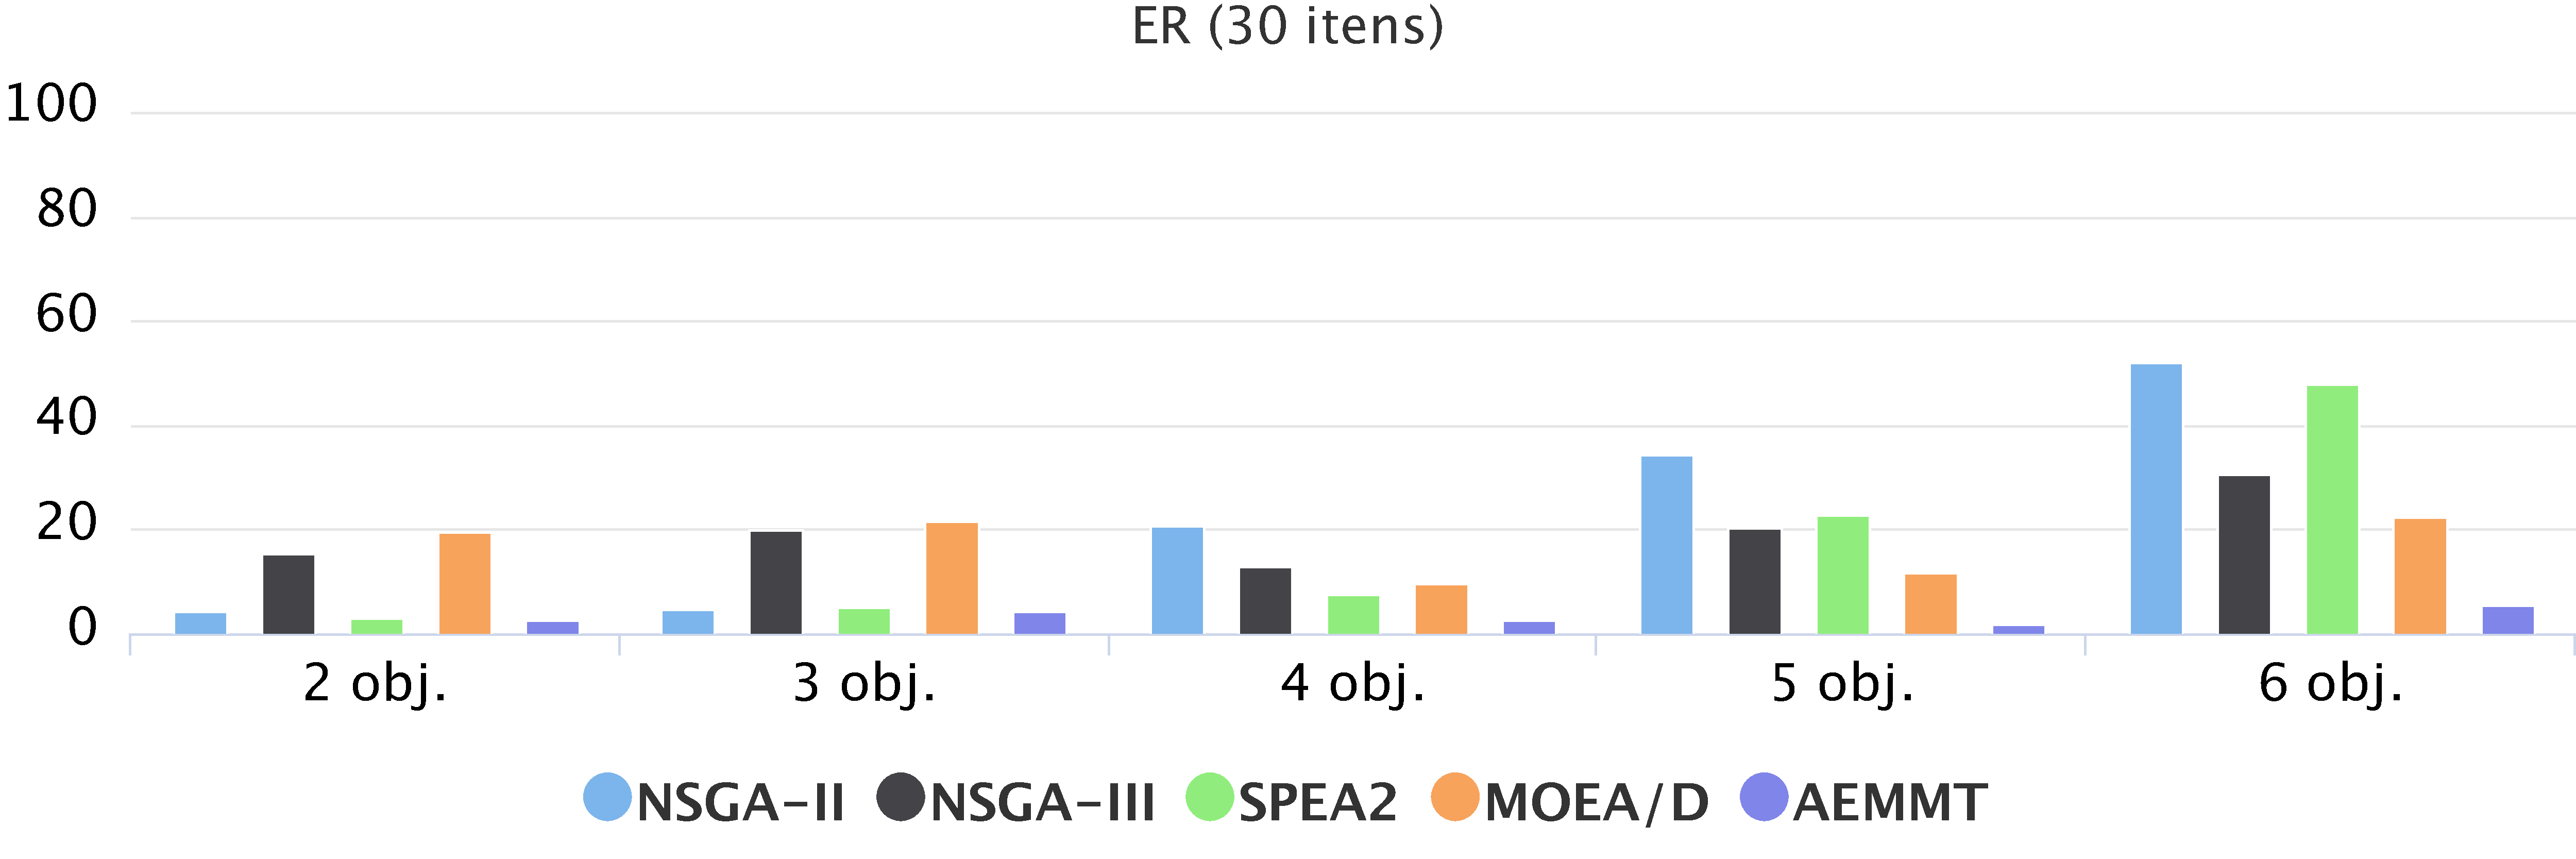
\includegraphics[width=1\textwidth]{cap_experimentos/figs/etapa1/er-mkp-30}
	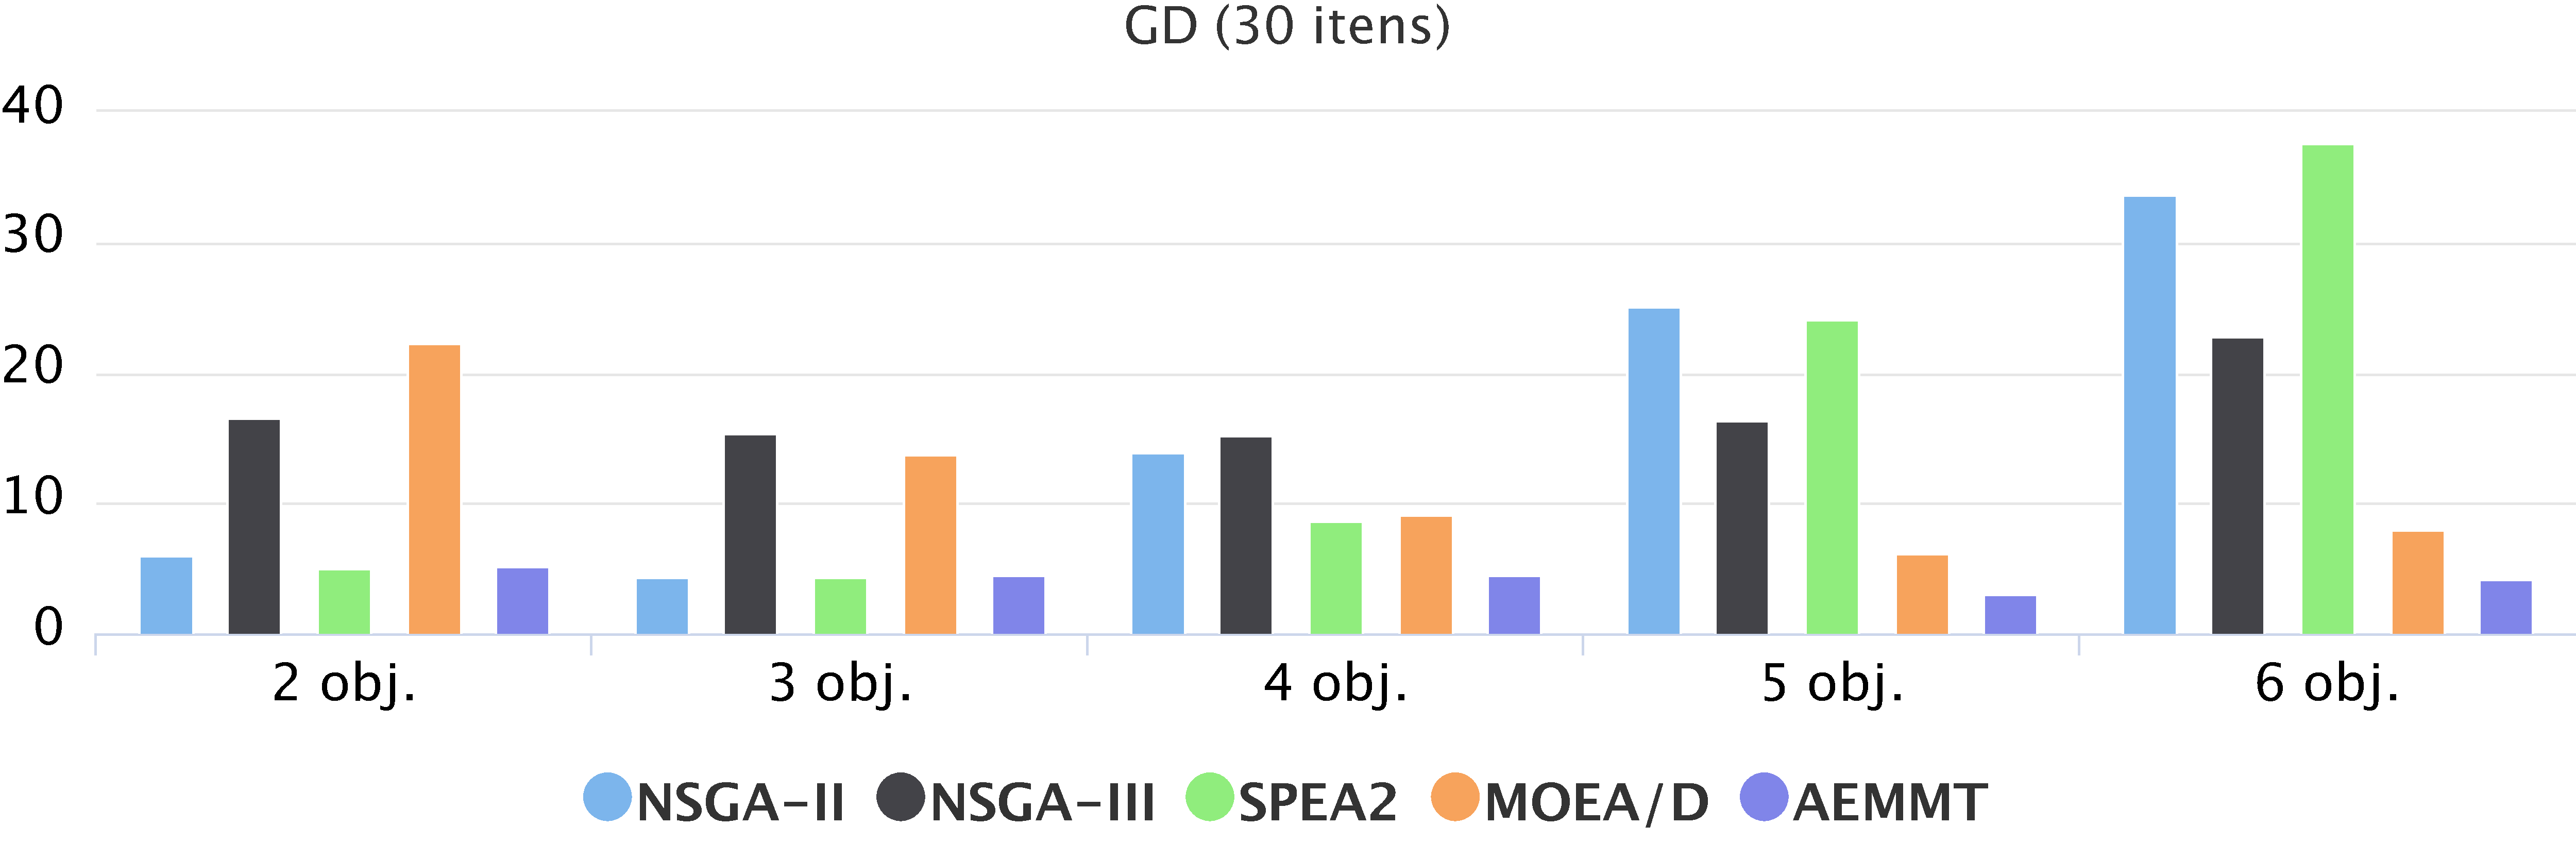
\includegraphics[width=1\textwidth]{cap_experimentos/figs/etapa1/gd-mkp-30}
	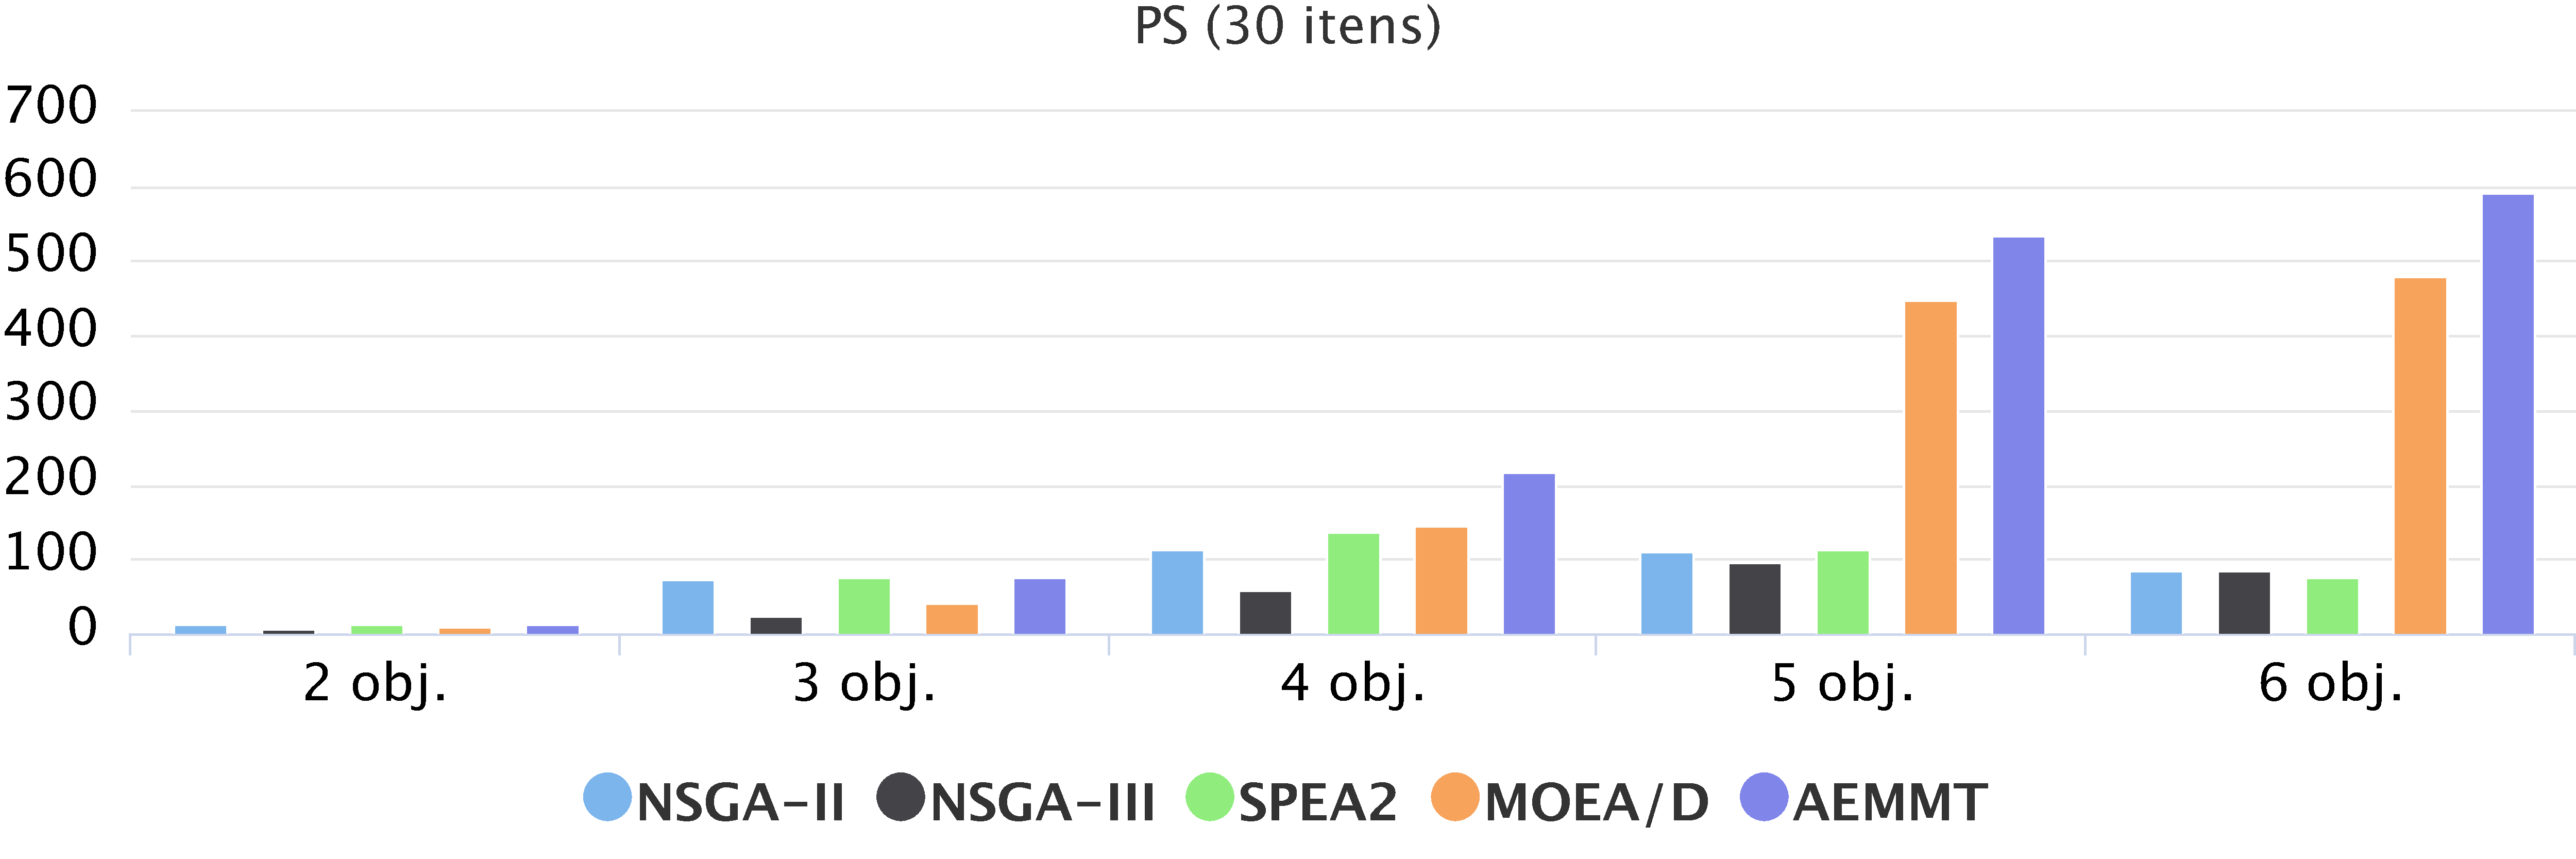
\includegraphics[width=1\textwidth]{cap_experimentos/figs/etapa1/ps-mkp-30}
	\caption{\label{fig_exp1_pmm_30}Desempenho dos algoritmos na 1ª etapa para o PMM com 30 itens}
\end{figure*}

Como pode ser observado na \autoref{fig_exp1_pmm_30}, o PMM com 30 itens é um problema relativamente simples e, no geral, os métodos de otimização multiobjetivo alcançam bons resultados. Até 4 objetivos, apenas o MOEA/D passou a marca de 20\% de erro. Para 2 e 3 objetivos, os algoritmos NSGA-II, SPEA2 e AEMMT apresentaram desempenhos muito similares, resultando nos melhores percentuais de erro entre todos os algoritmos avaliados. A partir de 4 objetivos é possível notar uma piora considerável nos algoritmos multiobjetivos clássicos (NSGA-II e SPEA-2). Considerando todas as formulações de objetivo, os melhores resultados foram obtidos pelo AEMMT que manteve o erro abaixo de 6\% em todos os casos. Analisando a métrica $GD$, obtém-se as mesmas conclusões tiradas a partir do $ER$. Isto é, considerando todas as formulações, o AEMMT gera os melhores resultados. Por outro lado, apesar de terem ótimo desempenho nos problemas de 2 e 3 objetivos, os valores da métrica GD para o NSGA-II e o SPEA2 apresentam resultados ruins a partir de 4 objetivos. O tamanho da fronteira de Pareto encontrada, medida pelo $PS$, é maior nos algoritmos MOEA/D e AEMMT. Esse comportamento é esperado, pois diferentemente dos demais AEMOs, esses dois algoritmos não aplicam uma limitação sobre o tamanho do Pareto. Considerando as valores das três métricas em todas as formulações de objetivos para o PMM de 30 itens, está claro que, no geral, o AEMMT é o melhor dentre os métodos testados.

\begin{figure*}[!htbp]
	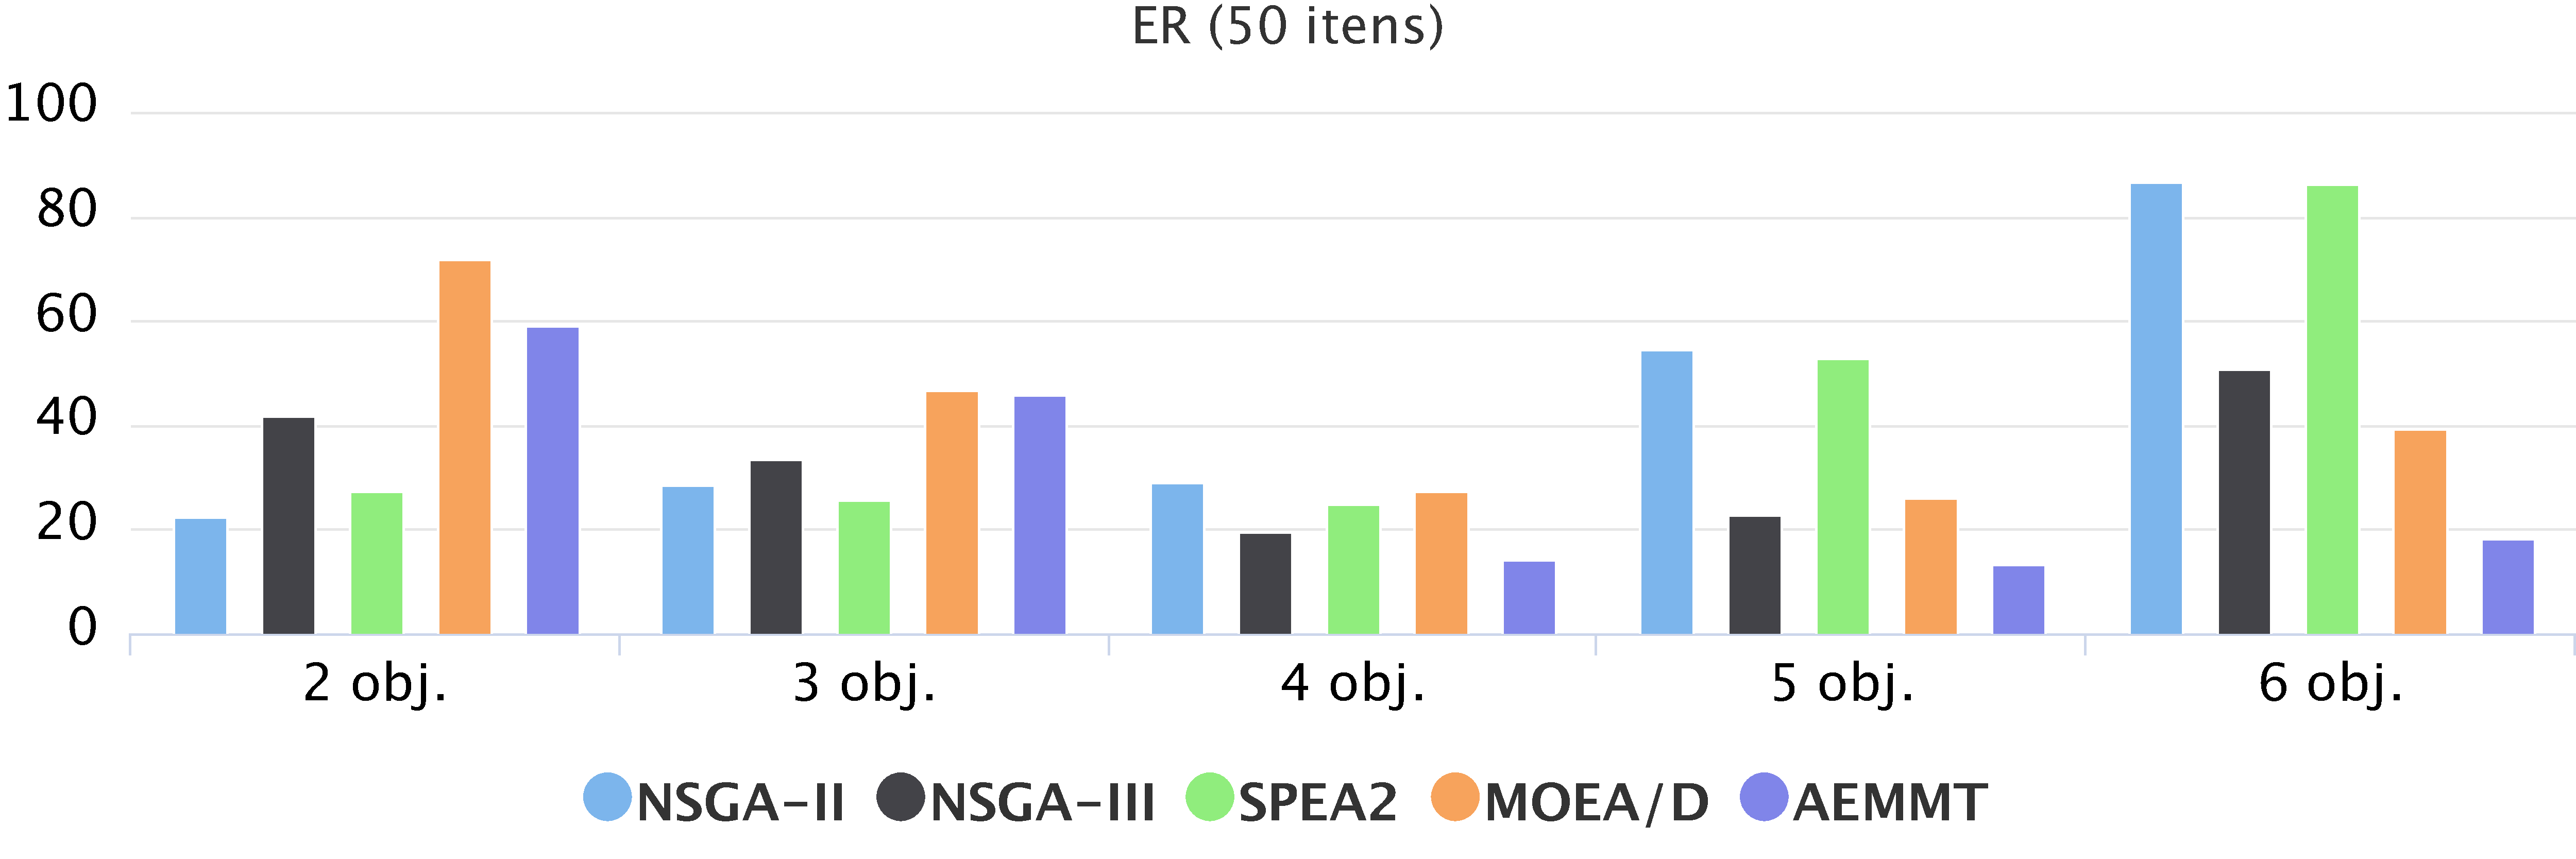
\includegraphics[width=1\textwidth]{cap_experimentos/figs/etapa1/er-mkp-50}
	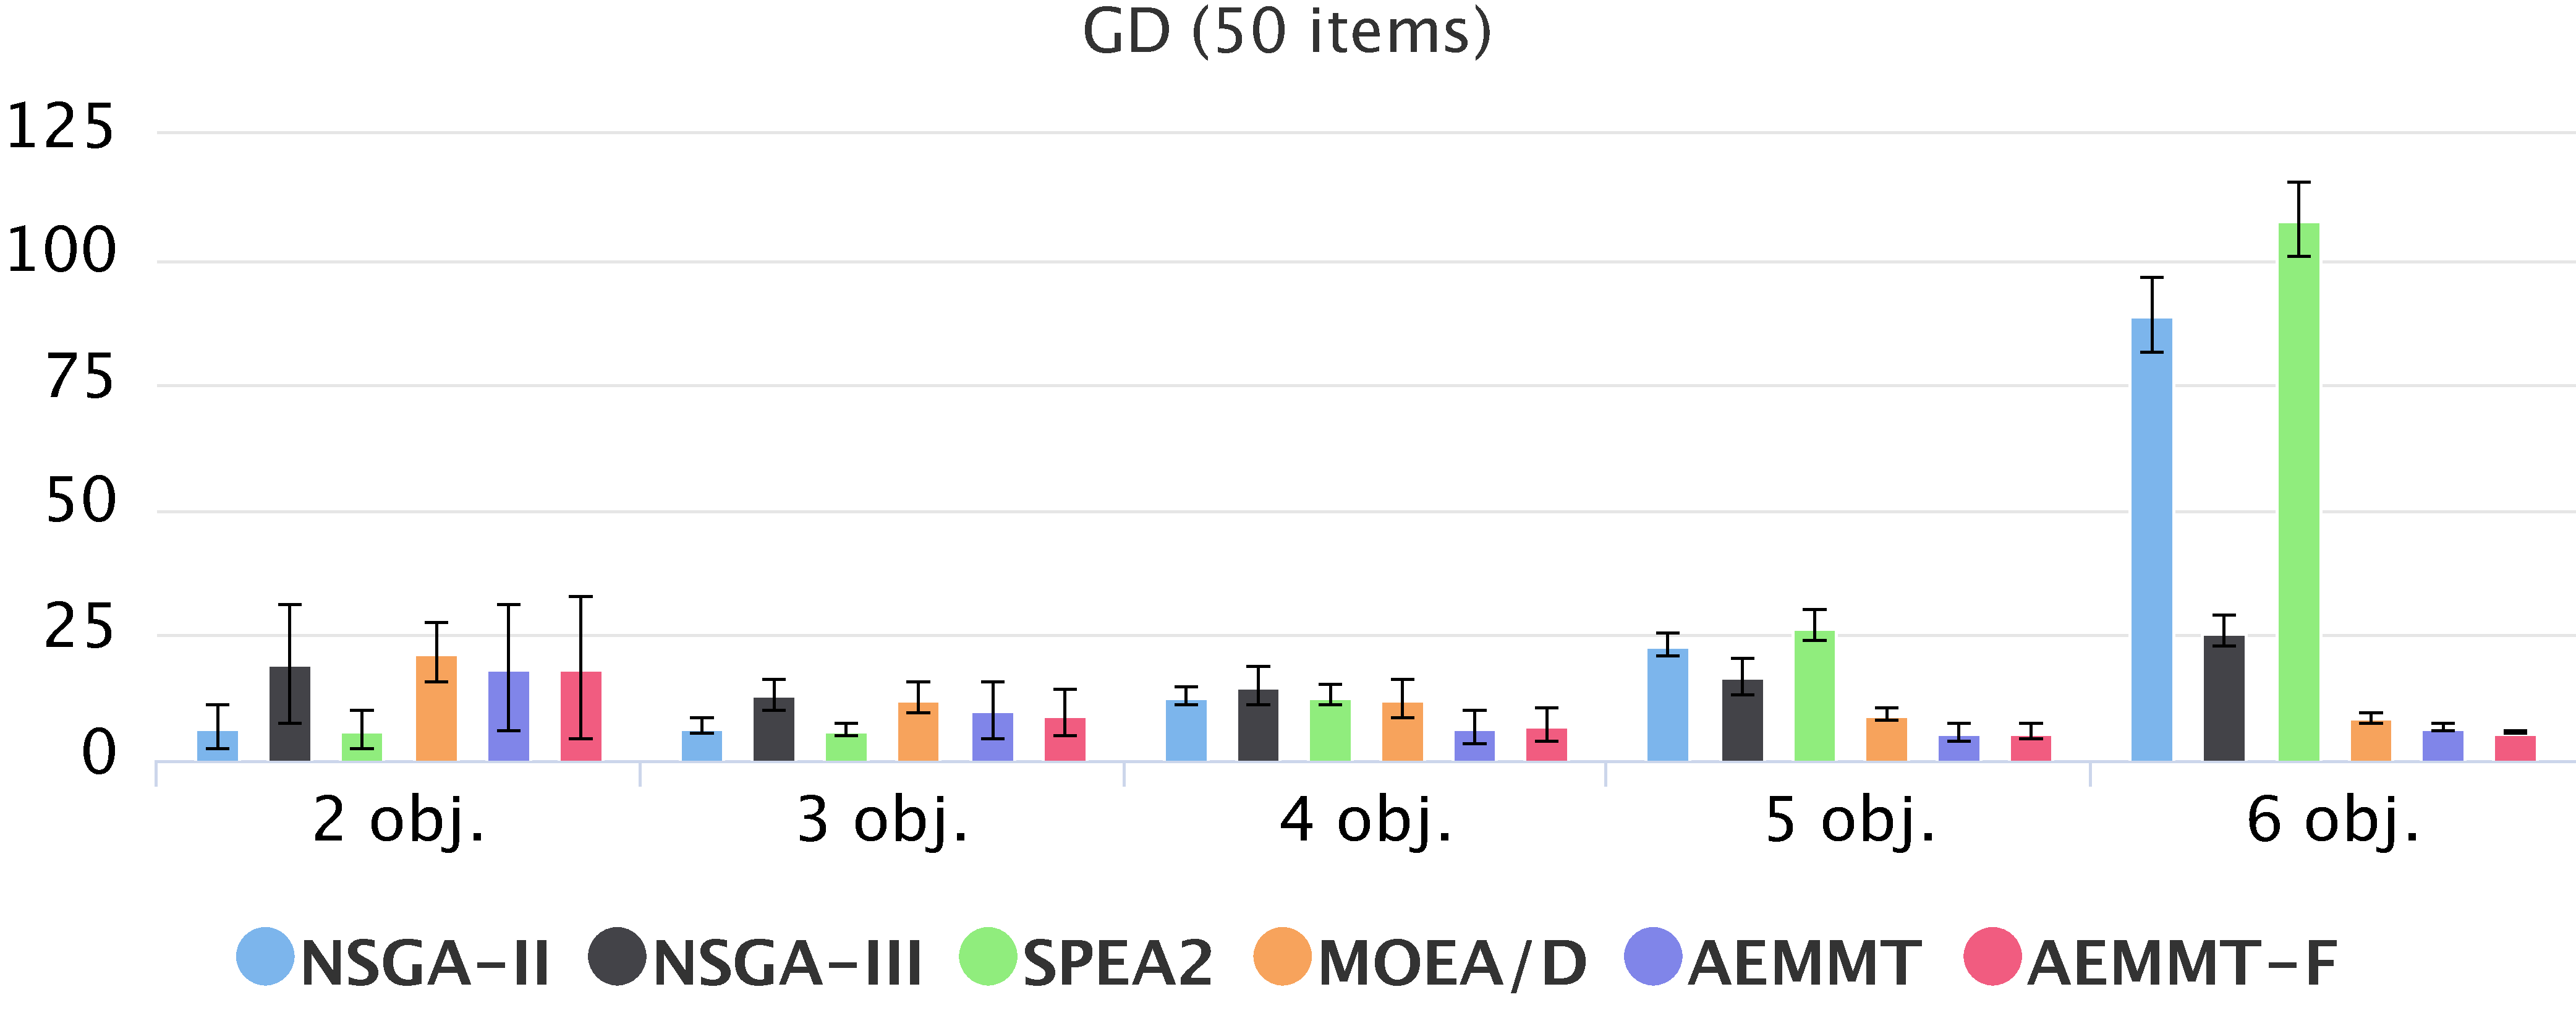
\includegraphics[width=1\textwidth]{cap_experimentos/figs/etapa1/gd-mkp-50}
	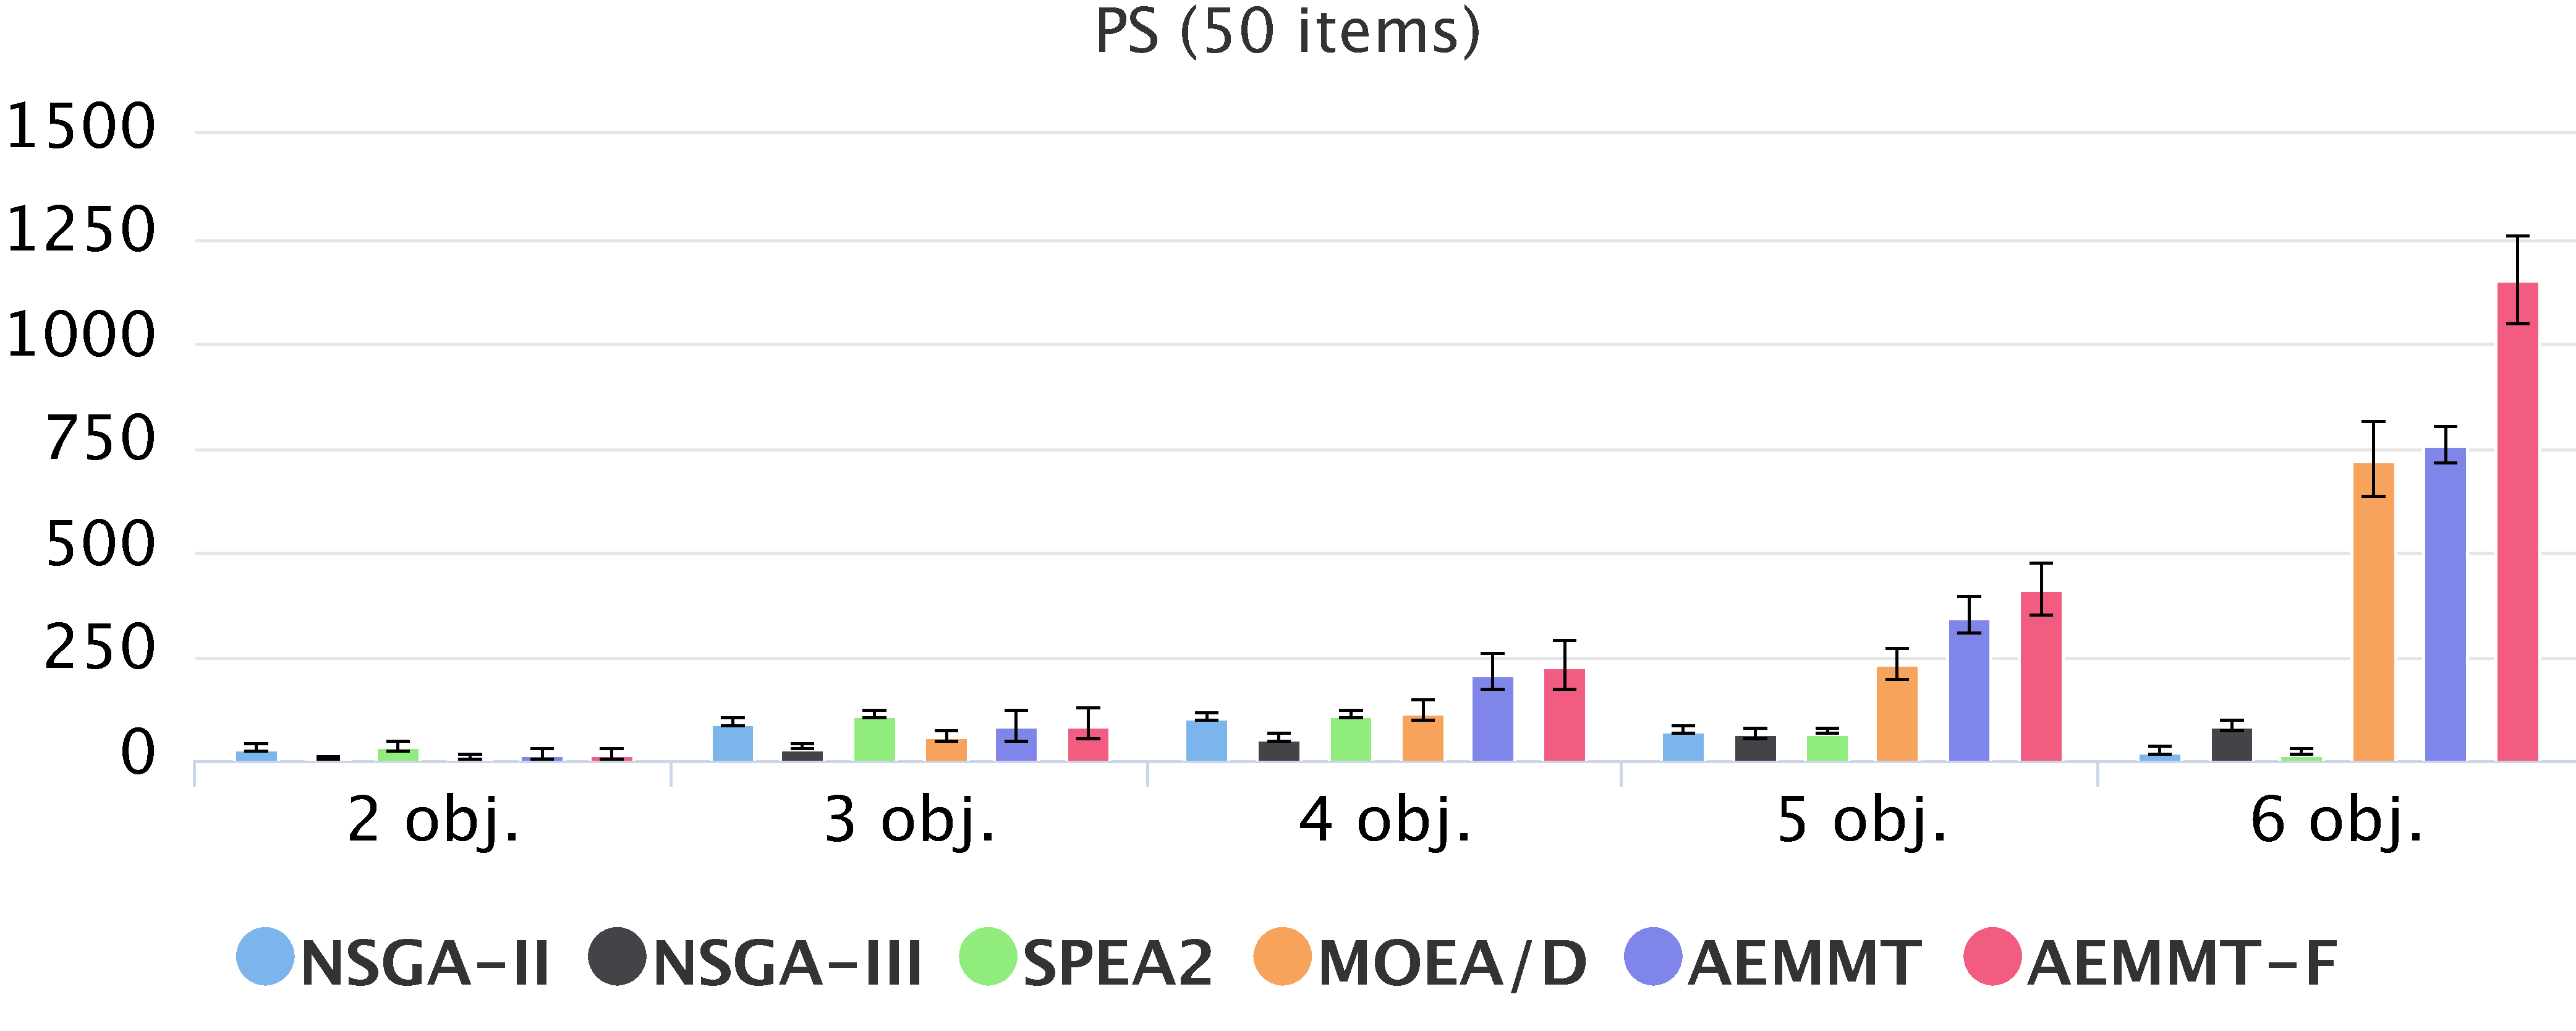
\includegraphics[width=1\textwidth]{cap_experimentos/figs/etapa1/ps-mkp-50}
	\caption{\label{fig_exp1_pmm_50}Desempenho dos algoritmos na 1ª etapa para o PMM com 50 itens}
\end{figure*}

O PMM com 50 itens (\autoref{fig_exp1_pmm_50}) é um problema bem mais complexo que sua versão com 30 itens. Nessa instância, é mais evidente  o comportamento de cada algoritmo em função das diferentes formulações de objetivos. Considerando as três métricas ($ER$, $GD$ e $PS$), os algoritmos clássicos (NSGA-II e SPEA2) são imbatíveis nas formulações com 2 e 3 objetivos. A partir de 4 objetivos, o AEMMT passa a apresentar melhores resultados. É possível notar que, com o aumento do número de objetivos, o NSGA-II e o SPEA2 pioram enquanto o AEMMT mantém o $ER$ e o $GD$ estáveis e melhora o $PS$. O MOEA/D é o segundo melhor algoritmo para problemas \textit{many-objectives} e o NSGA-III é o terceiro. Para o PMM de 50 itens, o AEMMT continua sendo a melhor opção.

\begin{figure*}[!htbp]
	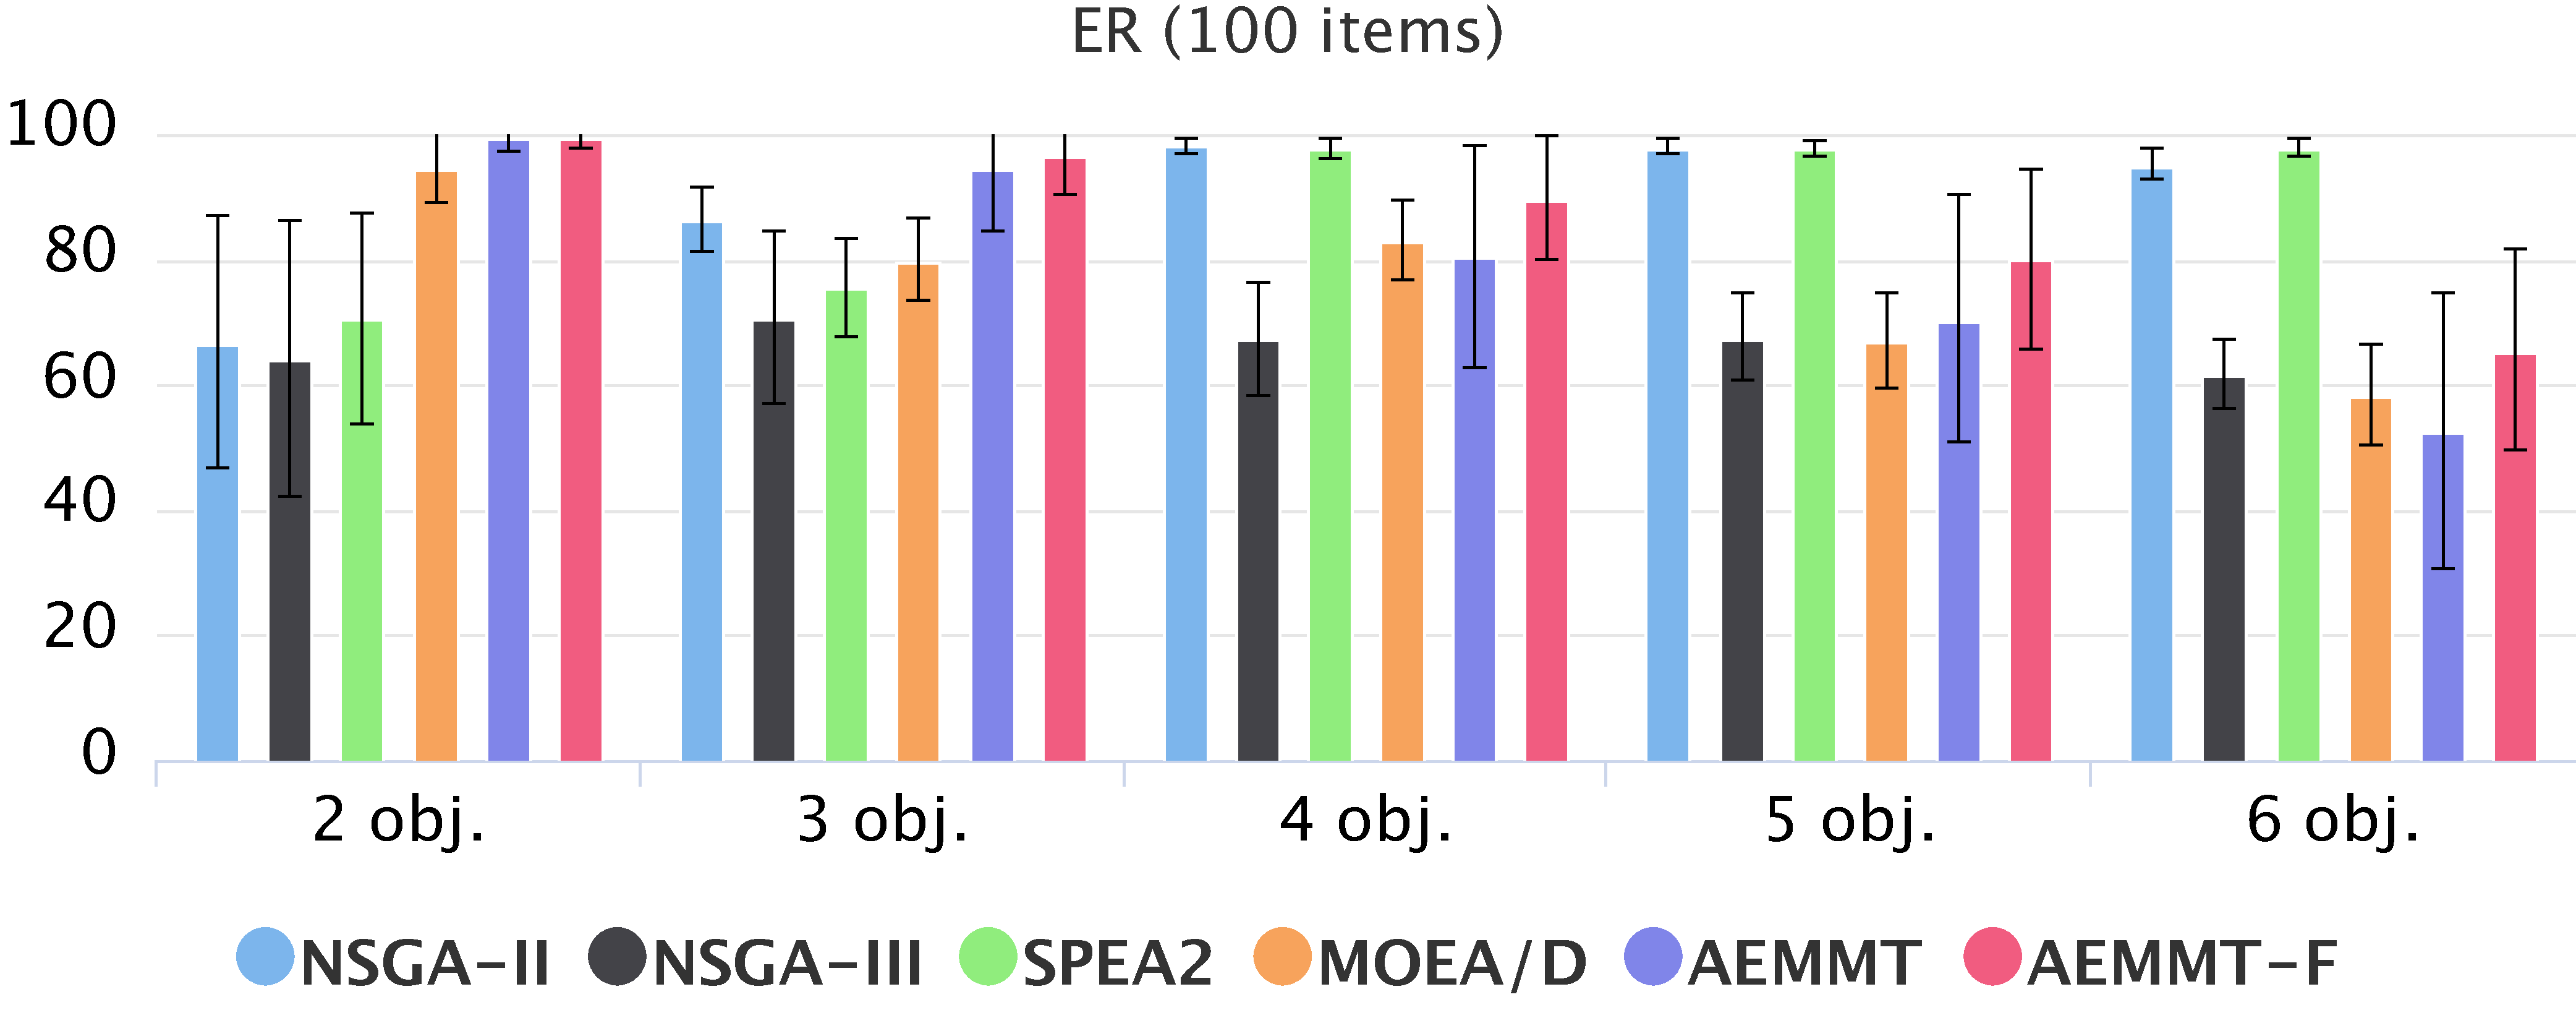
\includegraphics[width=1\textwidth]{cap_experimentos/figs/etapa1/er-mkp-100}
	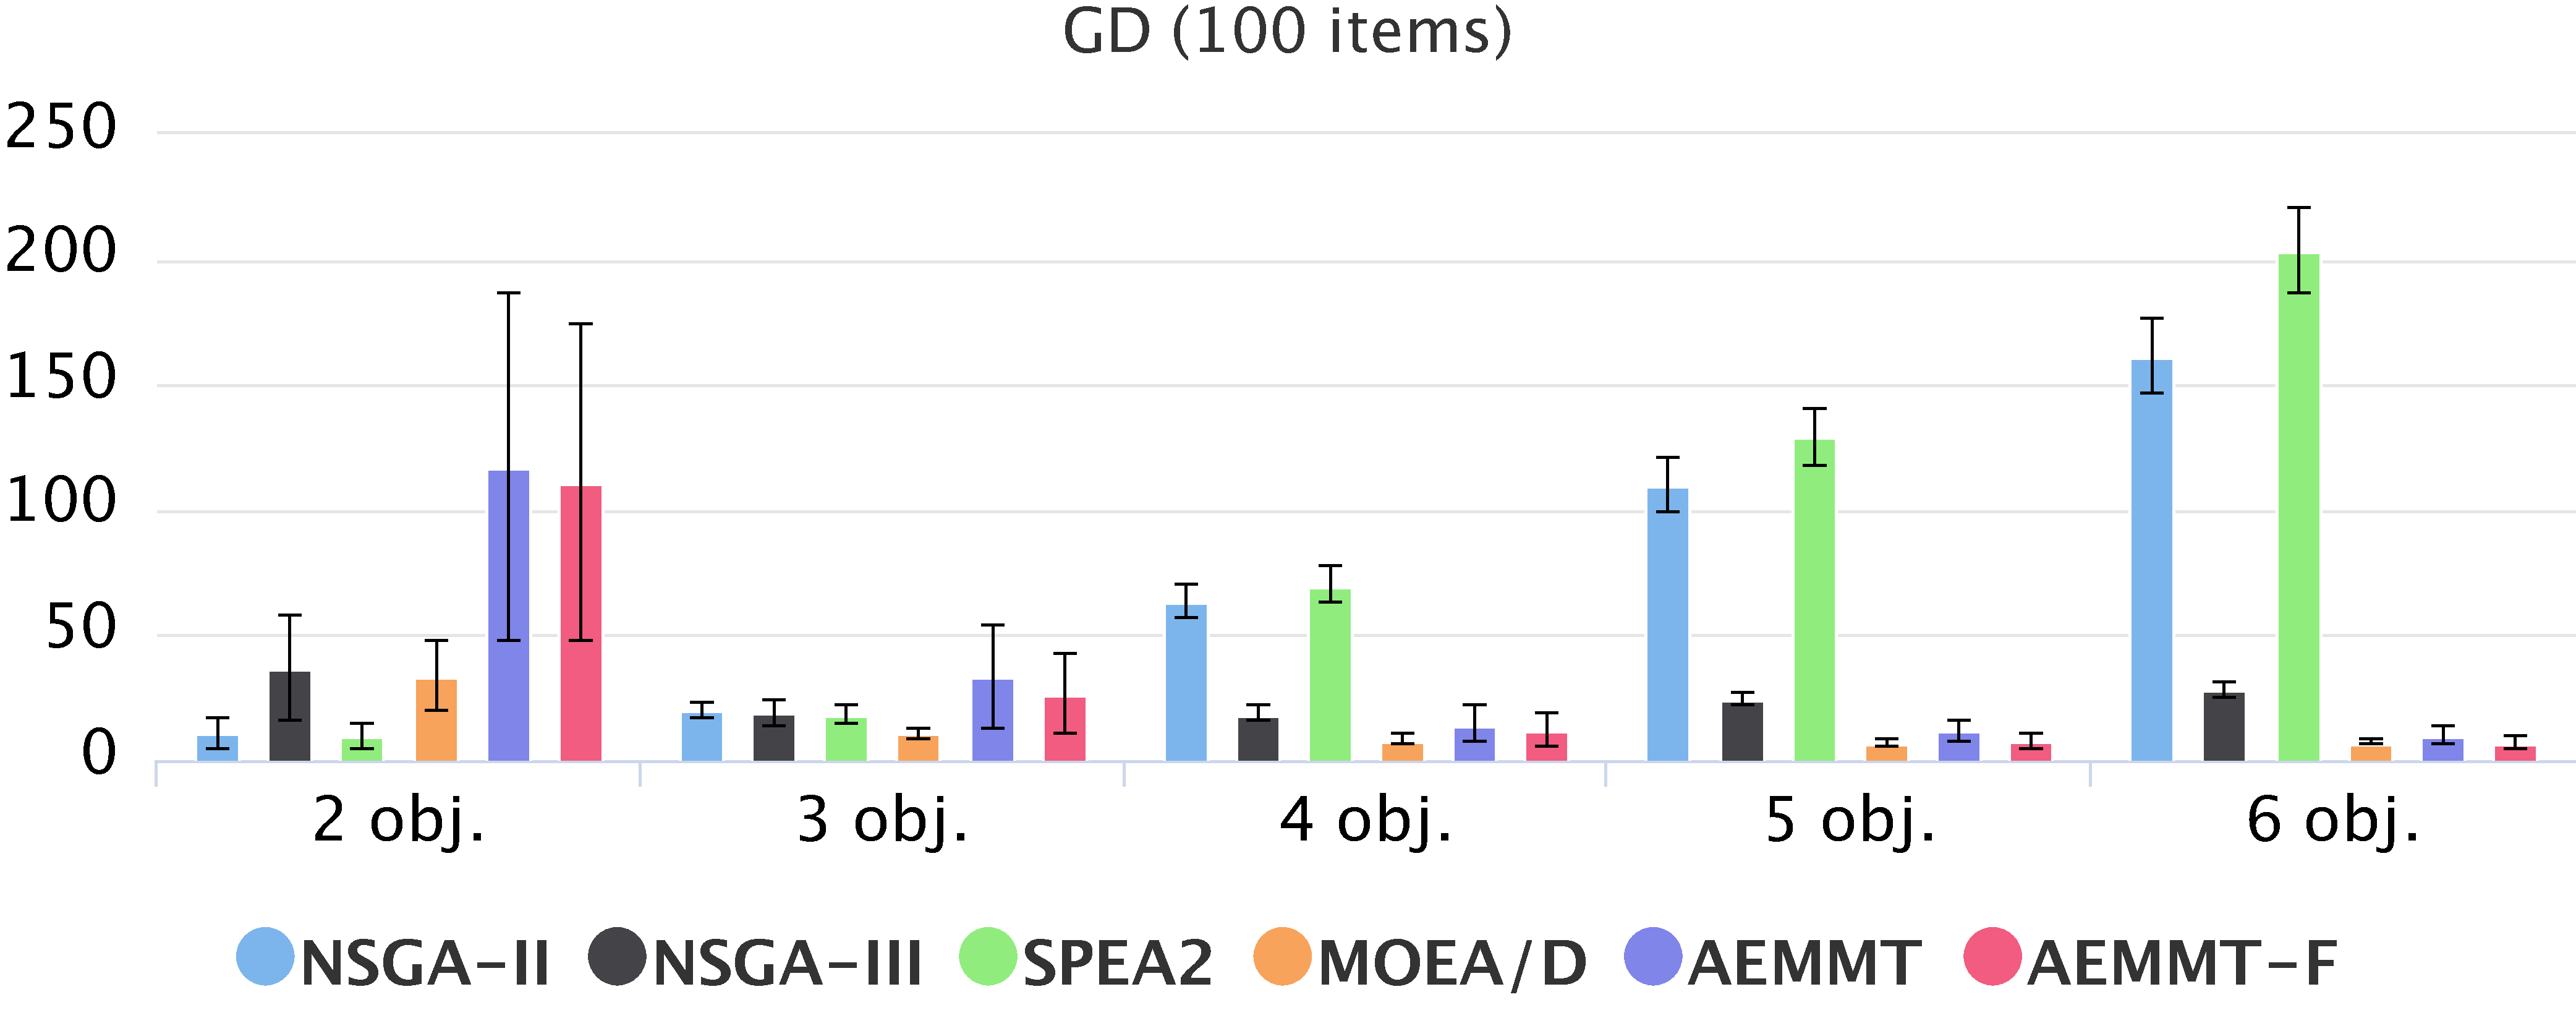
\includegraphics[width=1\textwidth]{cap_experimentos/figs/etapa1/gd-mkp-100}
	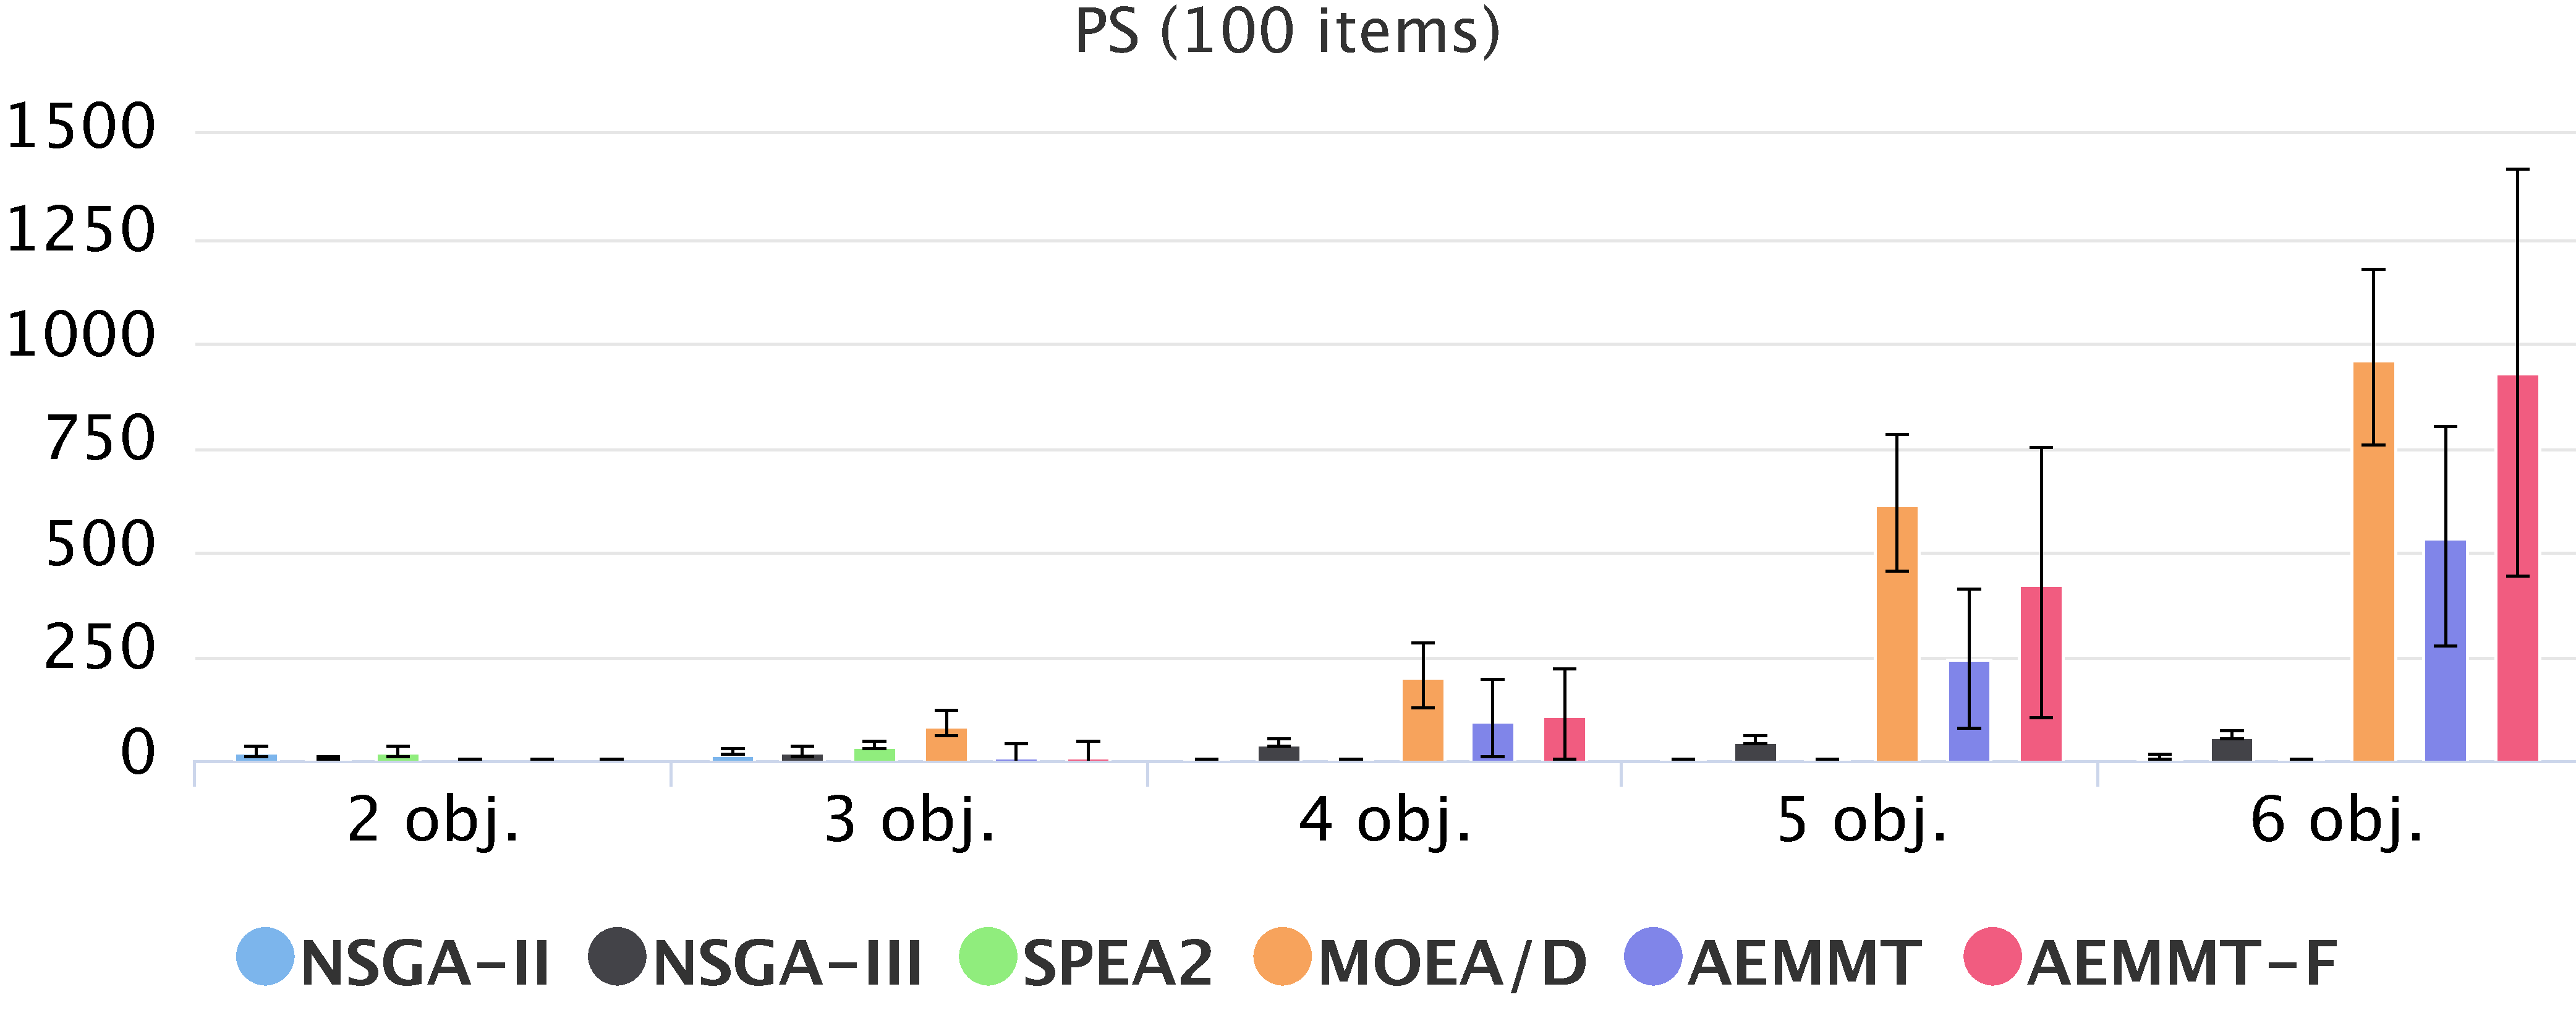
\includegraphics[width=1\textwidth]{cap_experimentos/figs/etapa1/ps-mkp-100}
	\caption{\label{fig_exp1_pmm_100}Desempenho dos algoritmos na 1ª etapa para o PMM com 100 itens}
\end{figure*}

O tamanho do espaço de busca no problema da mochila é $2^n$, sendo $n$ o número de itens. Portanto, a complexidade do PMM com 100 itens, cujos resultados são apresentados na \autoref{fig_exp1_pmm_100}, é muito maior que nas instâncias anteriores. Nesse caso, não foi possível encontrar um Pareto estável para as formulações de 4, 5 e 6 objetivos. Dessa forma, apesar de as métricas $ER$, $GD$ e $PS$ serem um bom indicativo do desempenho entre os algoritmos, a melhor forma de avaliação seria o hipervolume. Um experimento similar, mas utilizando o hipervolume, é apresentado na Seção \ref{section_experimentos_etapa4}. É difícil avaliar o problema considerando 100 itens, pois, a partir dos resultados apresentados para a métrica de erro (ER) na \autoref{fig_exp1_pmm_100}, é possível perceber que poucos algoritmos conseguiram encontrar boas soluções. Considerando a métrica $ER$, o algoritmo com melhor desempenho retornou uma taxa de erro acima de 50\%. O NSGA-III apresentou o menor $ER$ nos cenários de 2, 3, 4 e 5 objetivos, enquanto que na formulação de 6, os melhores desempenhos nessa métrica foram obtidos pelos AEMMT e MOEA/D. Com relação ao $GD$, o NSGA-II e o SPEA2 apresentaram os melhores resultados para 2 objetivos. Na formulação de 3 objetivos em diante, o MOEA/D foi o algoritmo com menor $GD$, sendo que , a partir de 4 objetivos, o AEMMT obteve desempenho similar. A situação se repete ao analisar o $PS$. A partir de 3 objetivos, o MOEA/D traz um conjunto maior de soluções na fronteira de Pareto, seguido pelo AEMMT a partir de 4 objetivos.

\begin{figure*}[!htbp]
	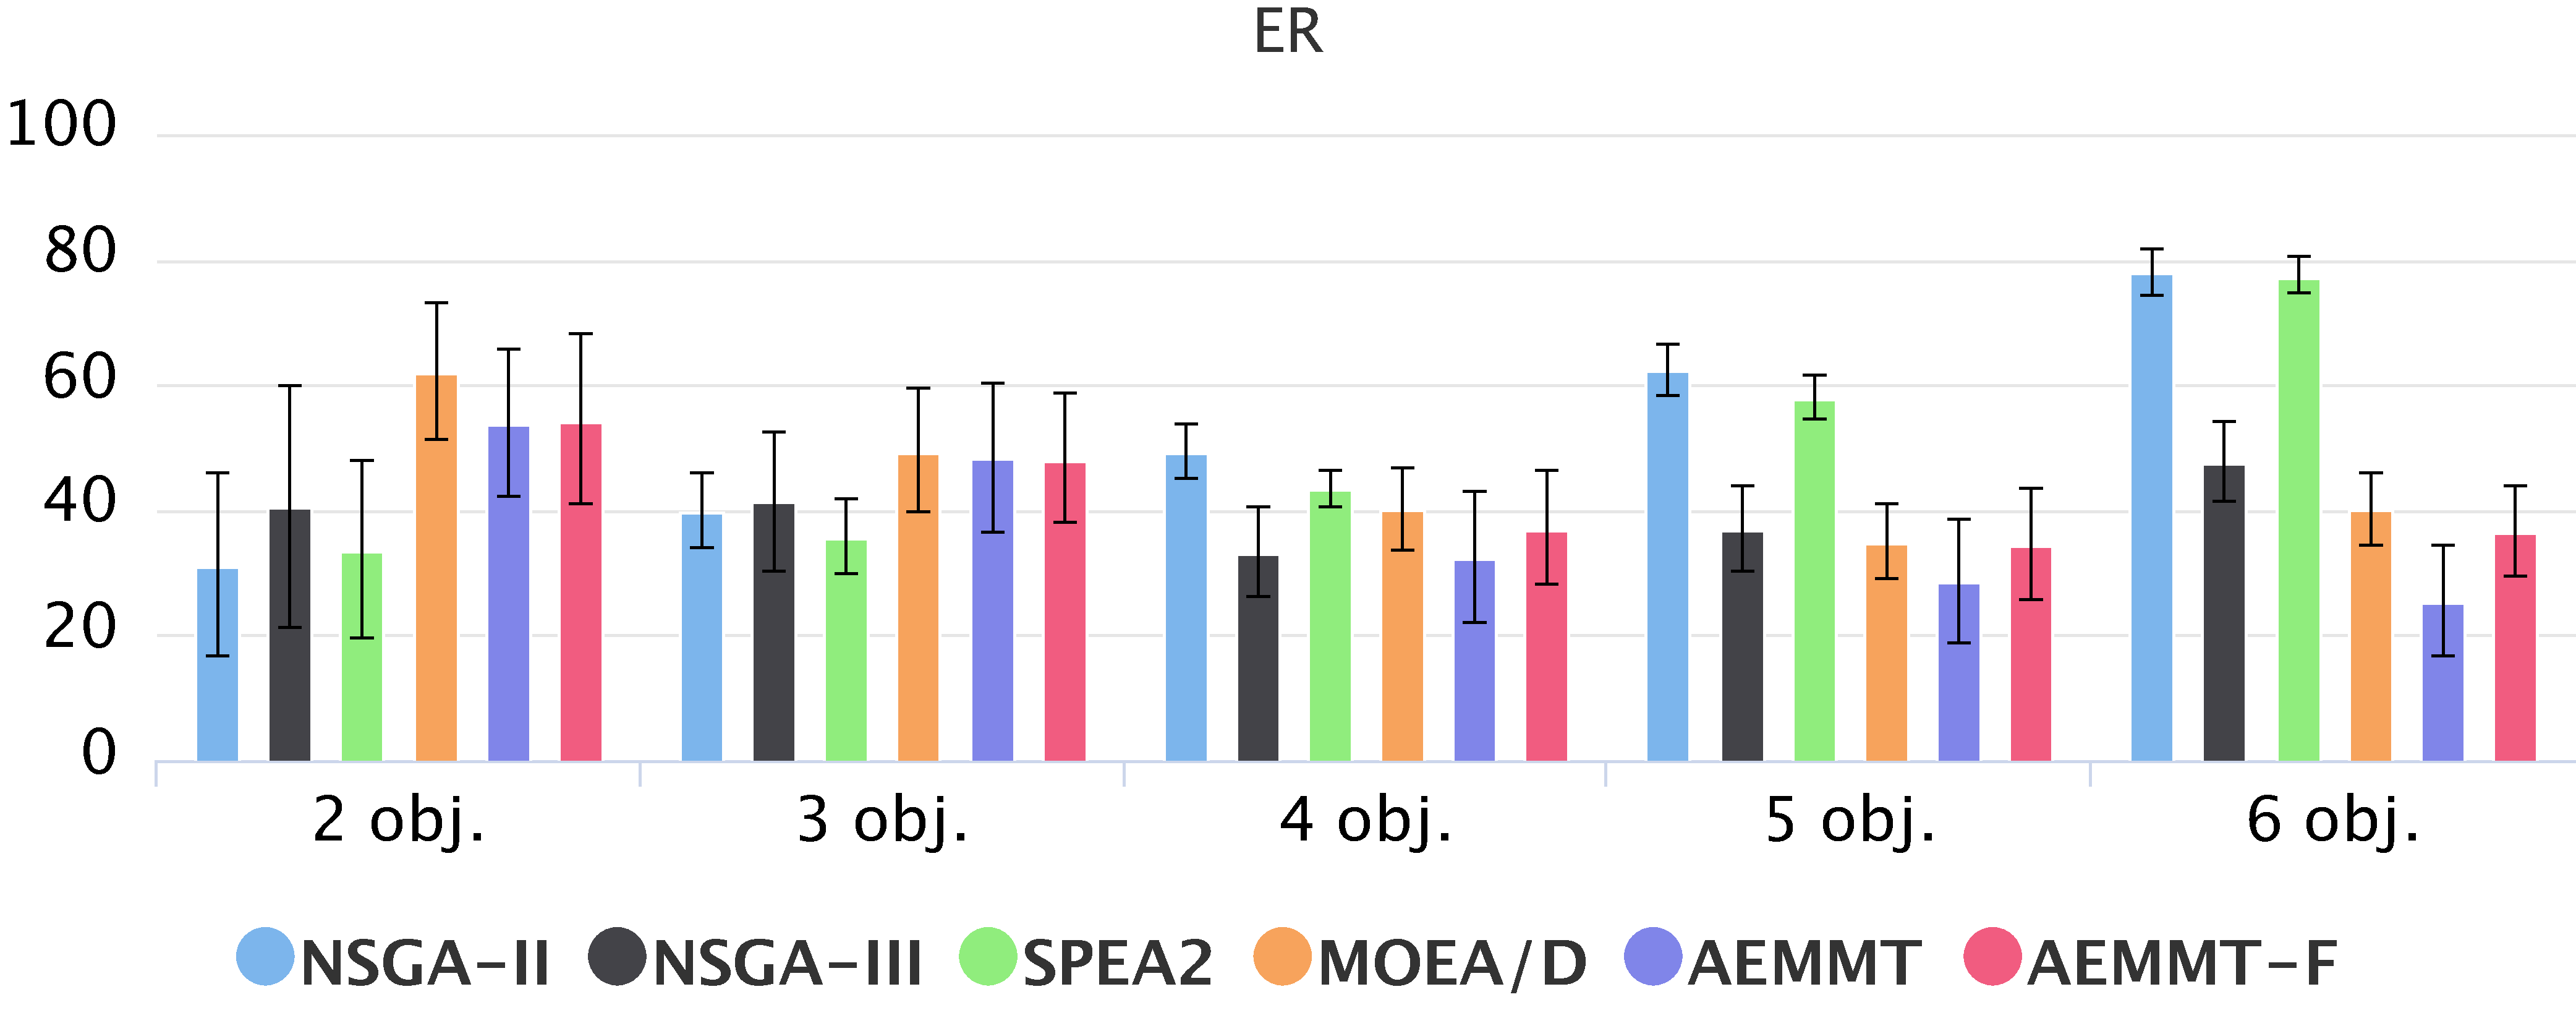
\includegraphics[width=1\textwidth]{cap_experimentos/figs/etapa1/er-mkp-todos}
	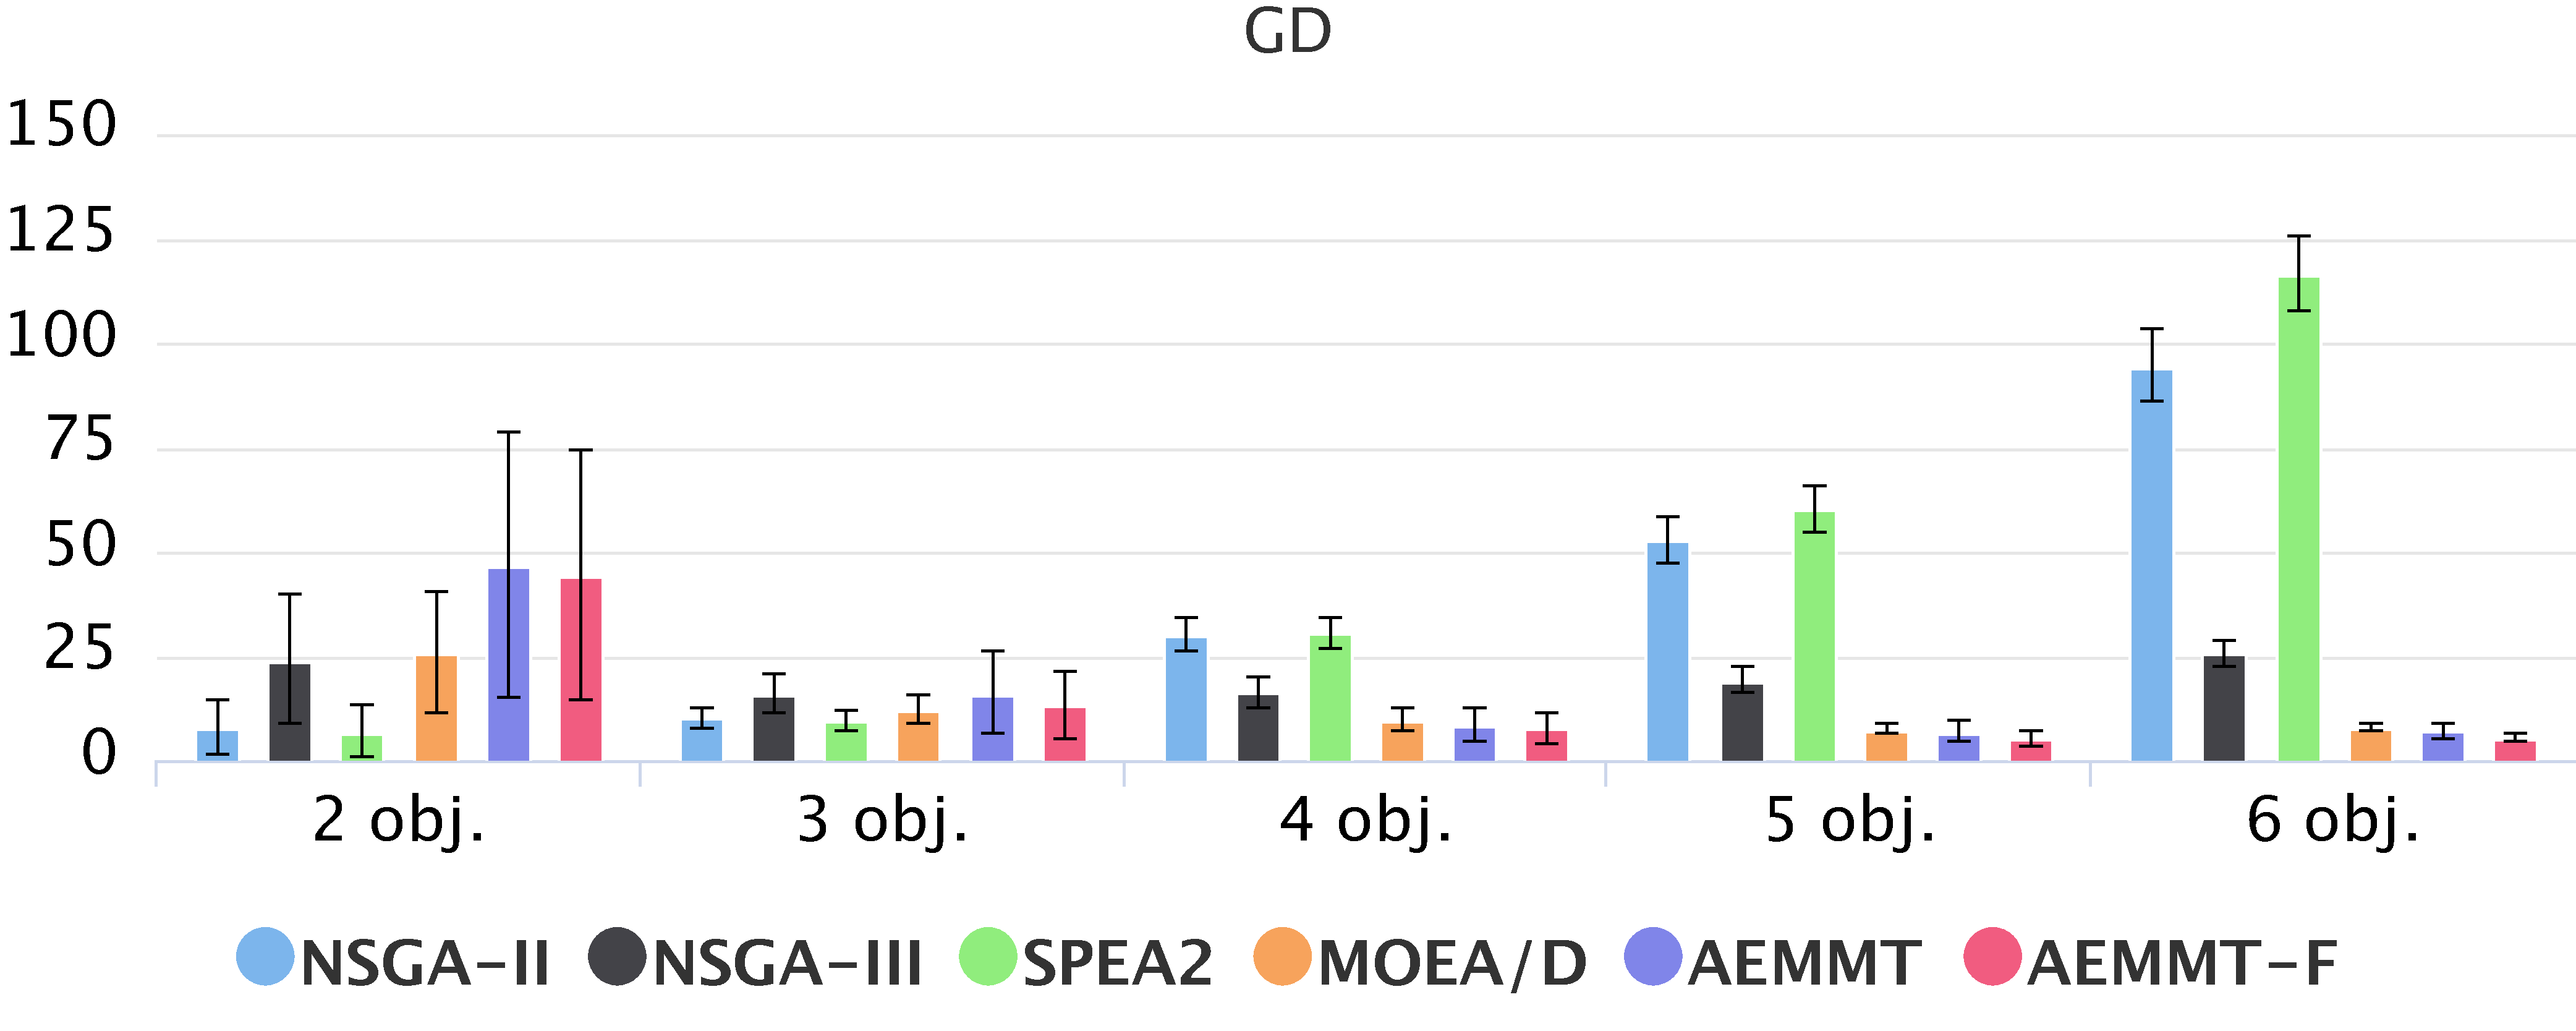
\includegraphics[width=1\textwidth]{cap_experimentos/figs/etapa1/gd-mkp-todos}
	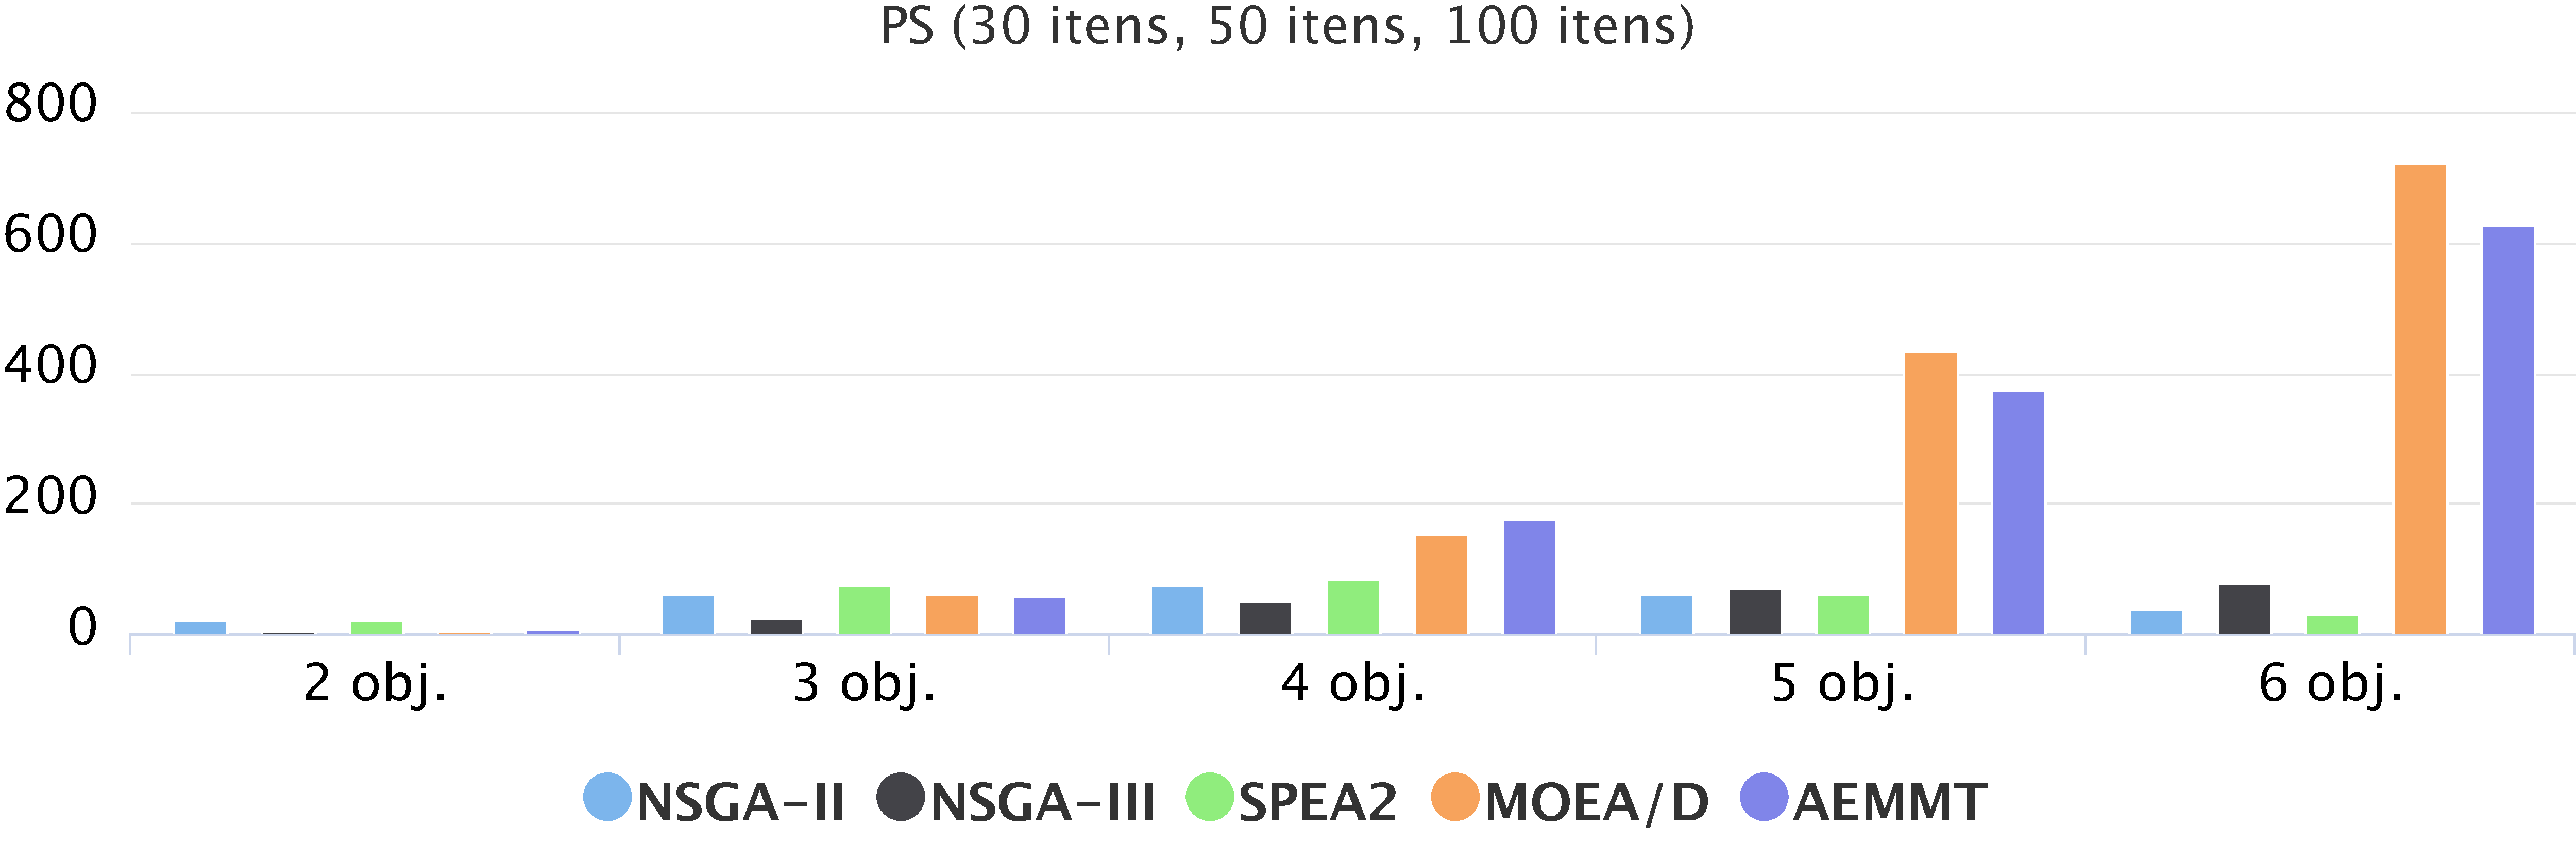
\includegraphics[width=1\textwidth]{cap_experimentos/figs/etapa1/ps-mkp-todos}
	\caption{\label{fig_exp1_pmm_todos}Resultado consolidado da 1ª etapa considerando o PMM com 30, 50 e 100 itens}
\end{figure*}

A \autoref{fig_exp1_pmm_100} apresenta os resultados do PMM de 30, 50 e 100 itens de forma consolidada para que se possa analisar, de forma geral, o comportamento dos algoritmos nas diferentes formulações de objetivo. Os gráficos representam as médias entre os três cenários de dificuldade (30, 50 e 100 itens). Como esperado, o NSGA-II e o SPEA2 são os melhores algoritmos para as formulações de 2 e 3 objetivos, tendo resultado nos melhores valores para as métricas $ER$, $GD$ e $PS$. Por outro lado, a partir de 4 objetivos, o desempenho de ambos os algoritmos cai consideravelmente, enquanto o AEMMT passa a apresentar os melhores resultados. O NSGA-III, no problema de 4 objetivos, apresenta um erro quase tão baixo quanto o AEMMT, mas seu $GD$ e $PS$ são piores. O MOEA/D, para 5 e 6 objetivos, apresenta o segundo melhor desempenho em qualquer uma das métricas. Em resumo, o NSGA-III não parece uma boa opção em nenhum dos casos, pois sempre há outro algoritmo que o supera. O NSGA-II e o SPEA2 são igualmente bons e os melhores em problemas com poucos objetivos. O AEMMT e o MOEA/D são ótimas opções para problemas a partir de 4 objetivos, sendo que o MOEA/D confere um melhor $PS$ enquanto o AEMMT proporciona uma menor taxa de erro.

\begin{figure*}[!htbp]
	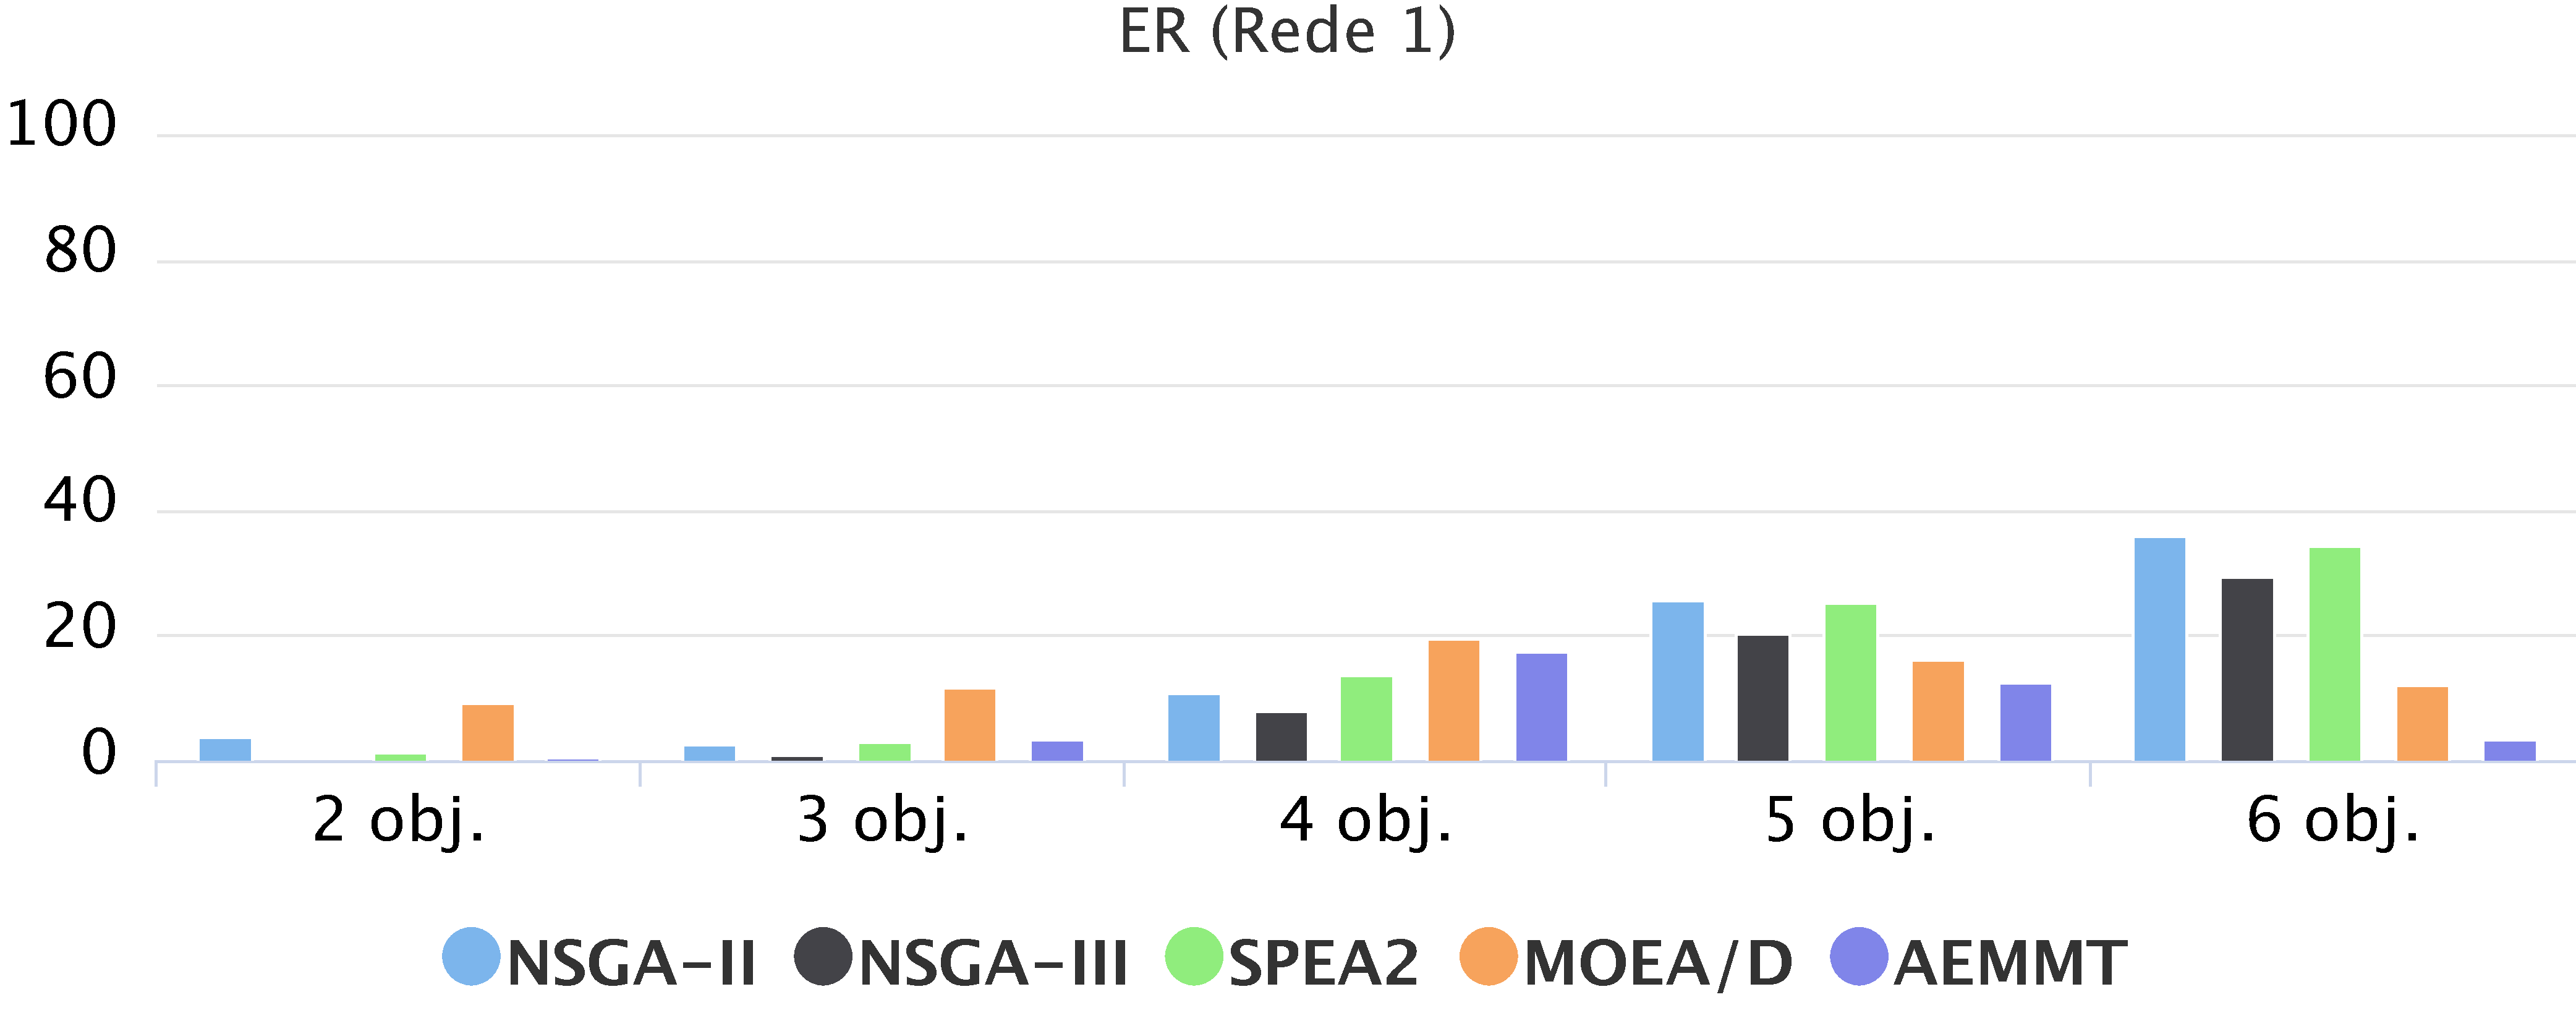
\includegraphics[width=1\textwidth]{cap_experimentos/figs/etapa1/er-mrp-r1}
	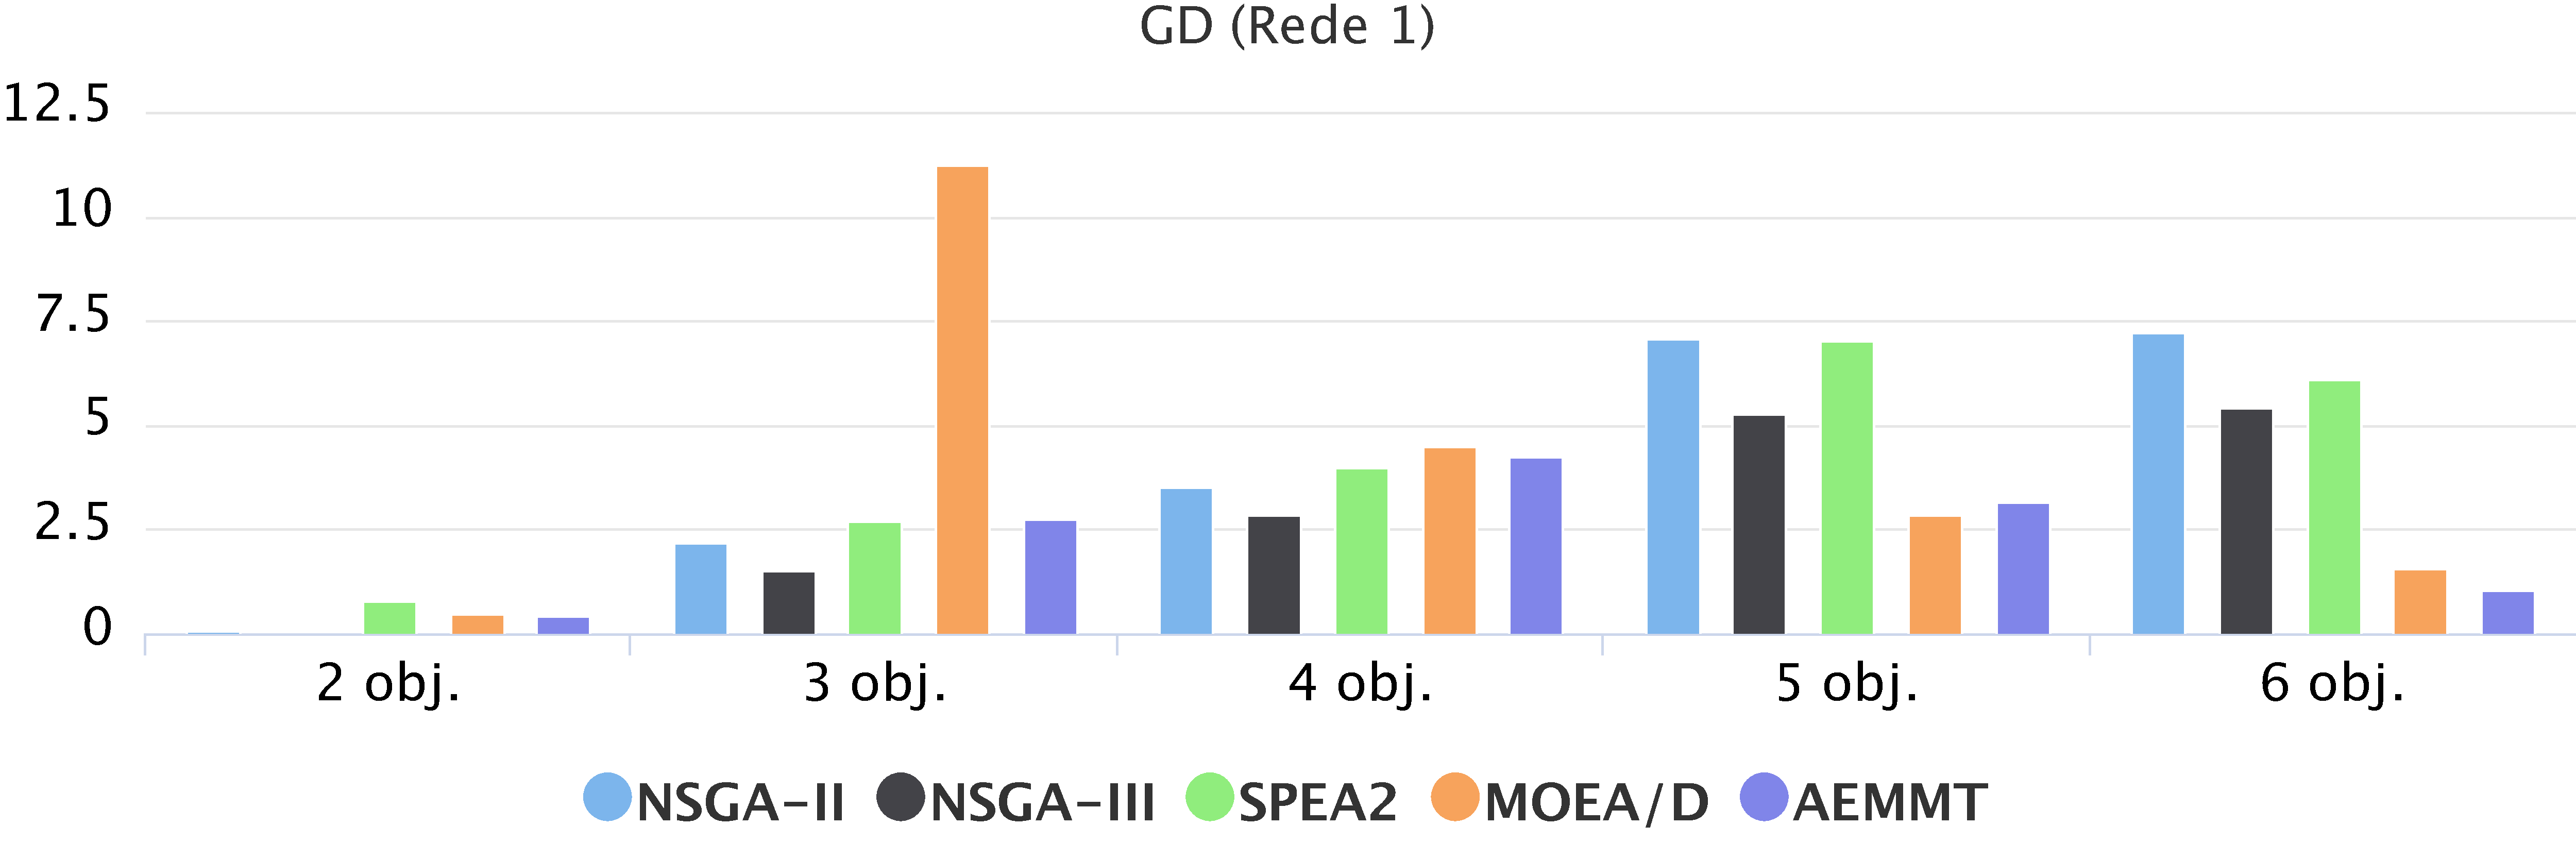
\includegraphics[width=1\textwidth]{cap_experimentos/figs/etapa1/gd-mrp-r1}
	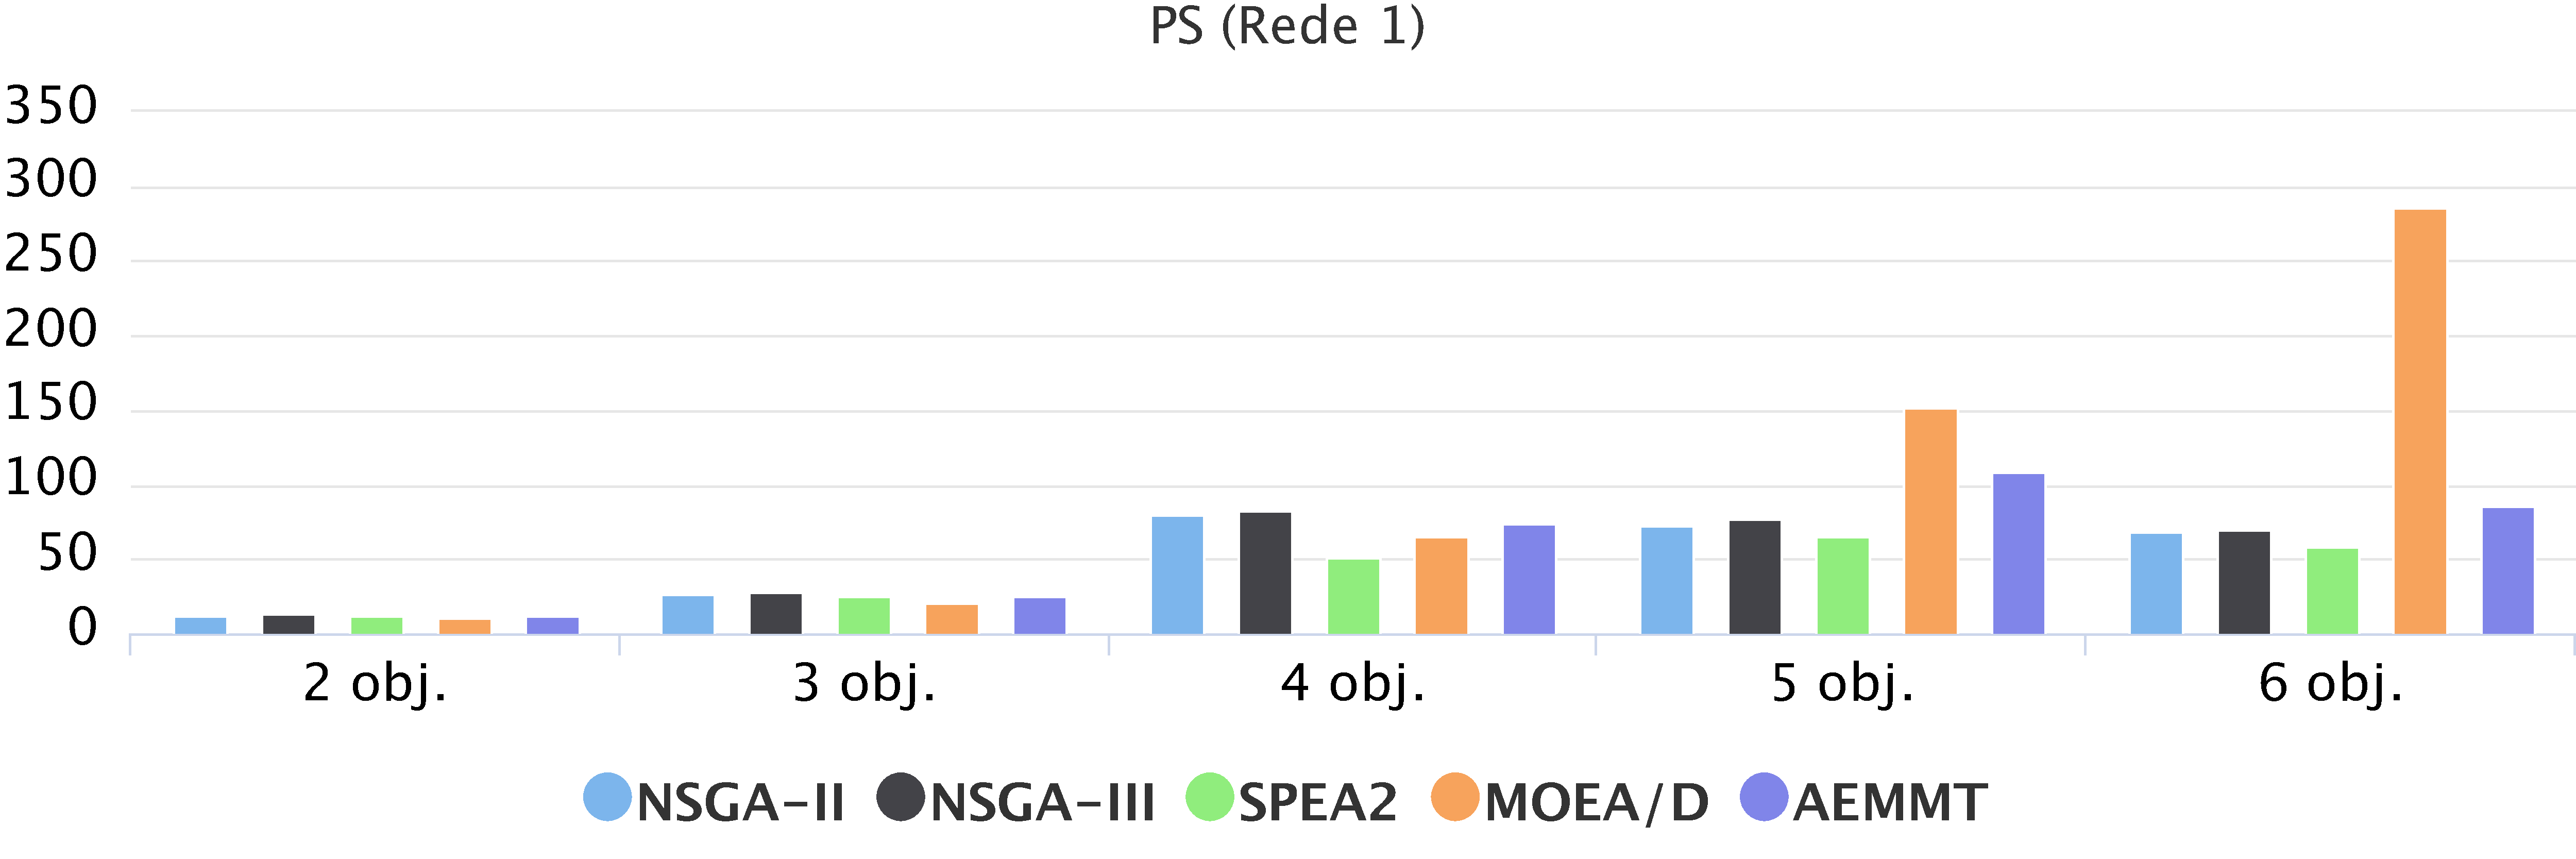
\includegraphics[width=1\textwidth]{cap_experimentos/figs/etapa1/ps-mrp-r1}
	\caption{\label{fig_exp1_prm_r1}Desempenho dos algoritmos na 1ª etapa para o PRM na rede 1}
\end{figure*}

Na \autoref{fig_exp1_prm_r1} são apresentados os desempenhos dos AEMOs na resolução do PRM para a rede 1. Essa é a instância mais simples testada e seu uso propiciou bons resultados para todos os algoritmos. Diferente do esperado, o NSGA-III mostrou o melhor resultado ($ER$, $GD$ e $PS$) para os problemas com 2, 3 e 4 objetivos. A partir de 5 objetivos, o AEMMT e o MOEA/D são os dois melhores métodos, o primeiro apresenta uma menor taxa de erro, enquanto o segundo obtém um Pareto de maior cardinalidade. Para poucos objetivos, o NSGA-III é claramente o melhor método, para 5 ou mais critérios de otimização, ambos AEMMT e MOEA/D são boas opções.

\begin{figure*}[!htbp]	
	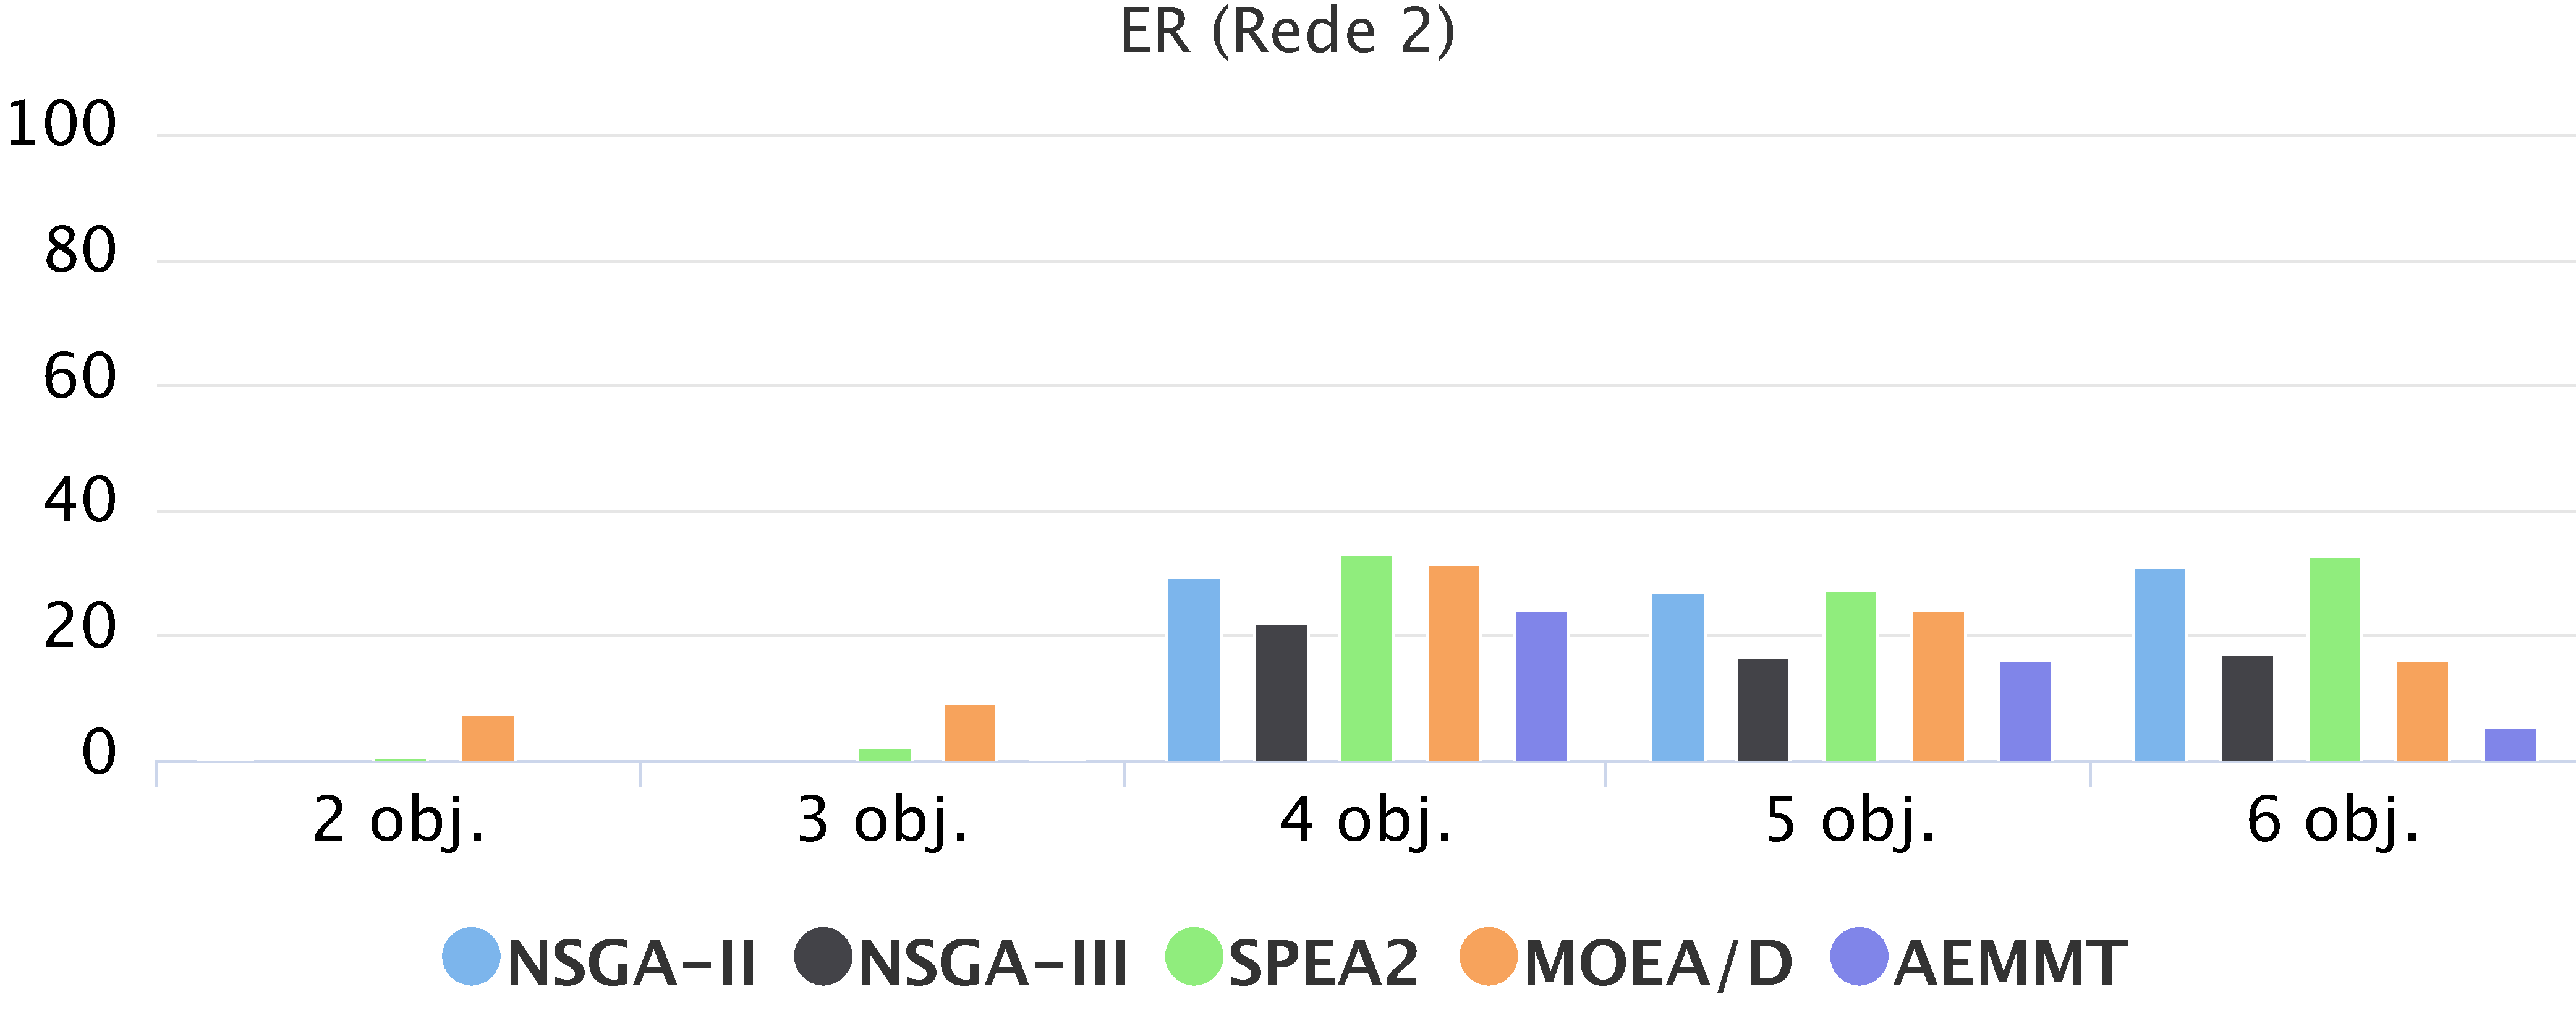
\includegraphics[width=1\textwidth]{cap_experimentos/figs/etapa1/er-mrp-r2}
	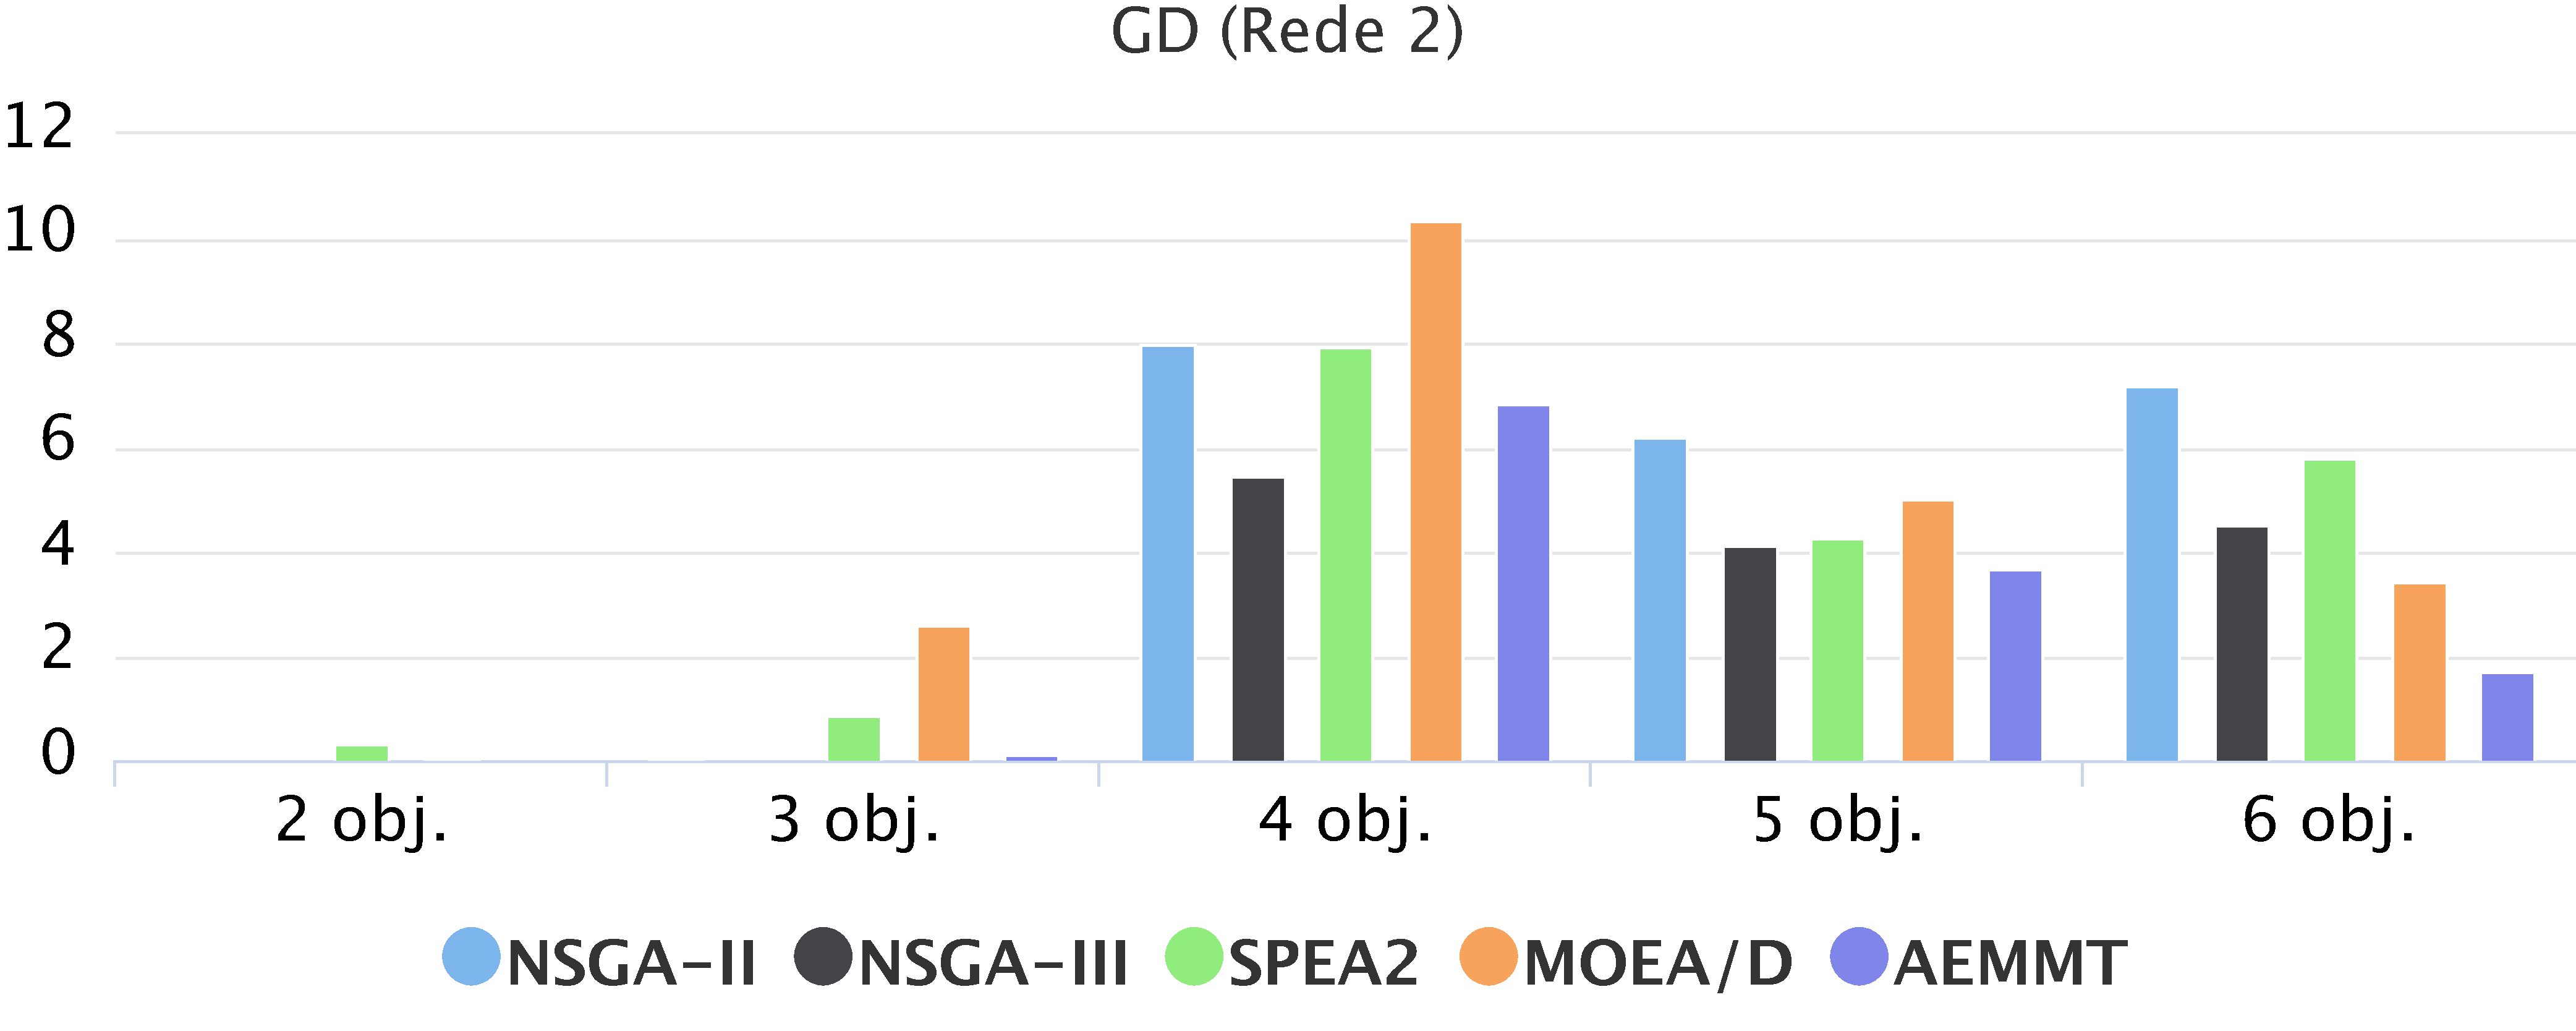
\includegraphics[width=1\textwidth]{cap_experimentos/figs/etapa1/gd-mrp-r2}
	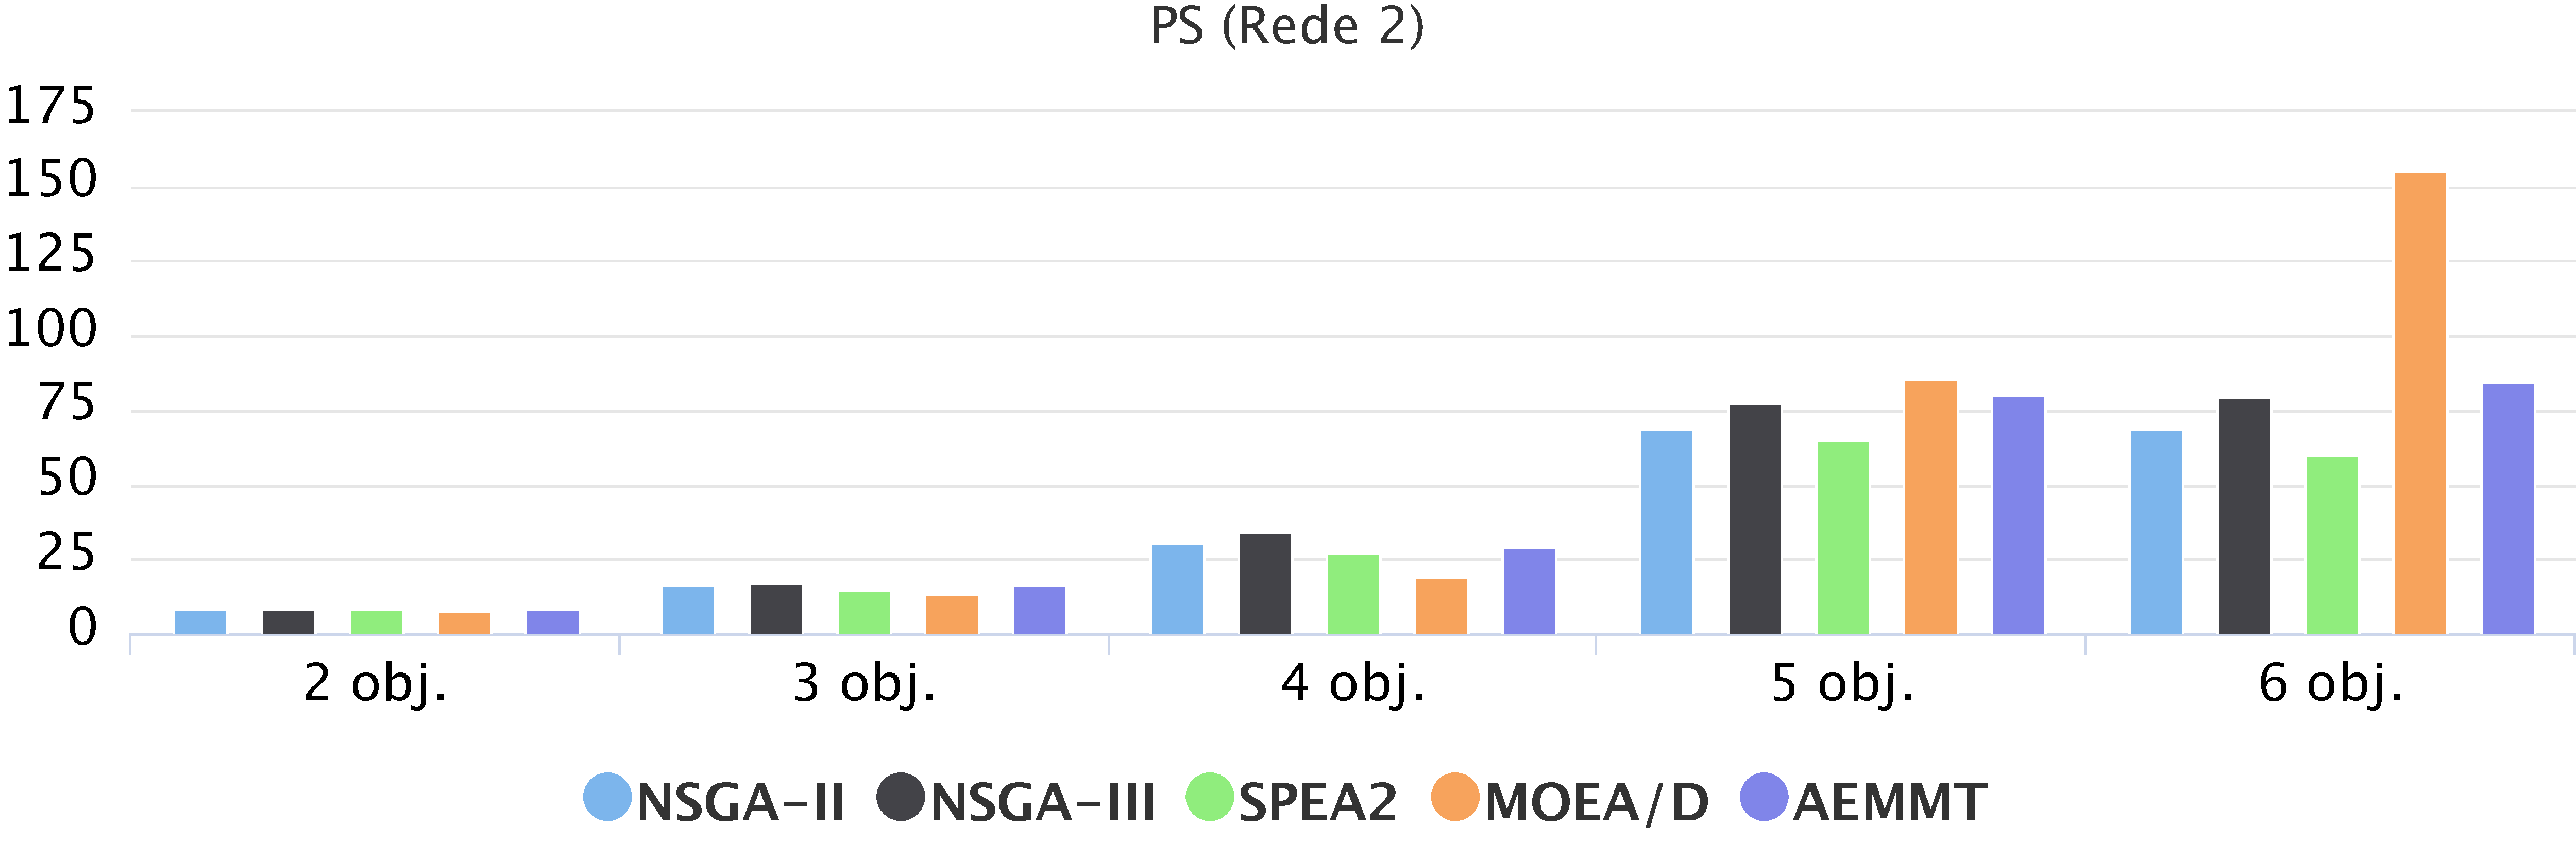
\includegraphics[width=1\textwidth]{cap_experimentos/figs/etapa1/ps-mrp-r2}
	\caption{\label{fig_exp1_prm_r2}Desempenho dos algoritmos na 1ª etapa para o PRM na rede 2}
\end{figure*}

Considerando o desempenho dos AEMOs para o PRM com a rede 2 (\autoref{fig_exp1_prm_r2}), o NSGA-III é o melhor algoritmo nos problemas com 2, 3, 4 e 5 objetivos, perdendo, por pouco, apenas em $PS$ para o AEMMT e o MOEA/D na formulação de 5 objetivos. Com 6 objetivos, o AEMMT é o melhor algoritmo quando se considera o erro e o $GD$, enquanto então o MOEA/D é o método mais adequado considerando a métrica $PS$.

\begin{figure*}[!htbp]
	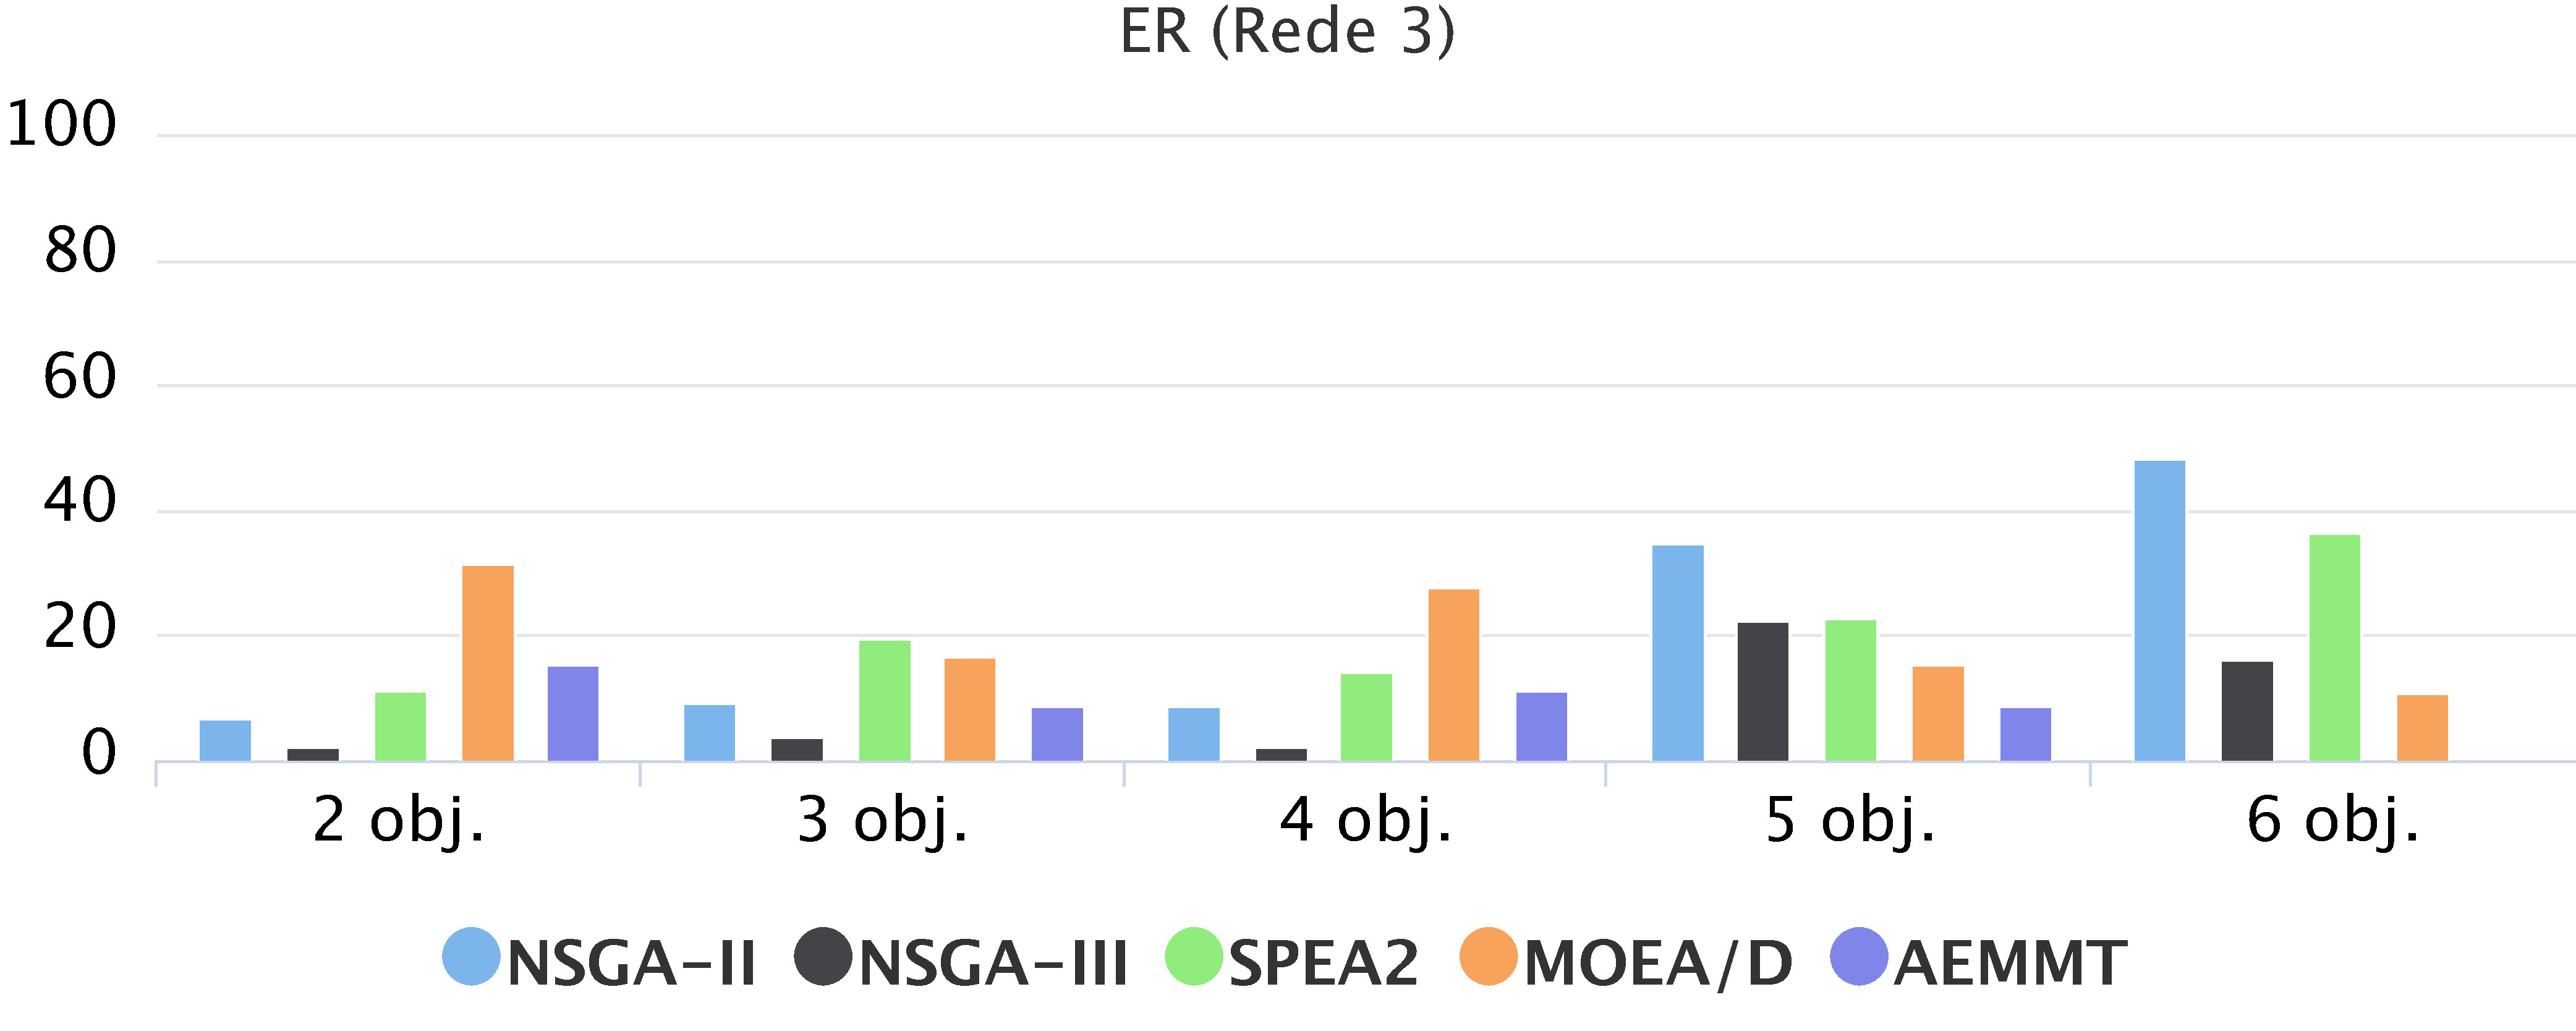
\includegraphics[width=1\textwidth]{cap_experimentos/figs/etapa1/er-mrp-r3}
	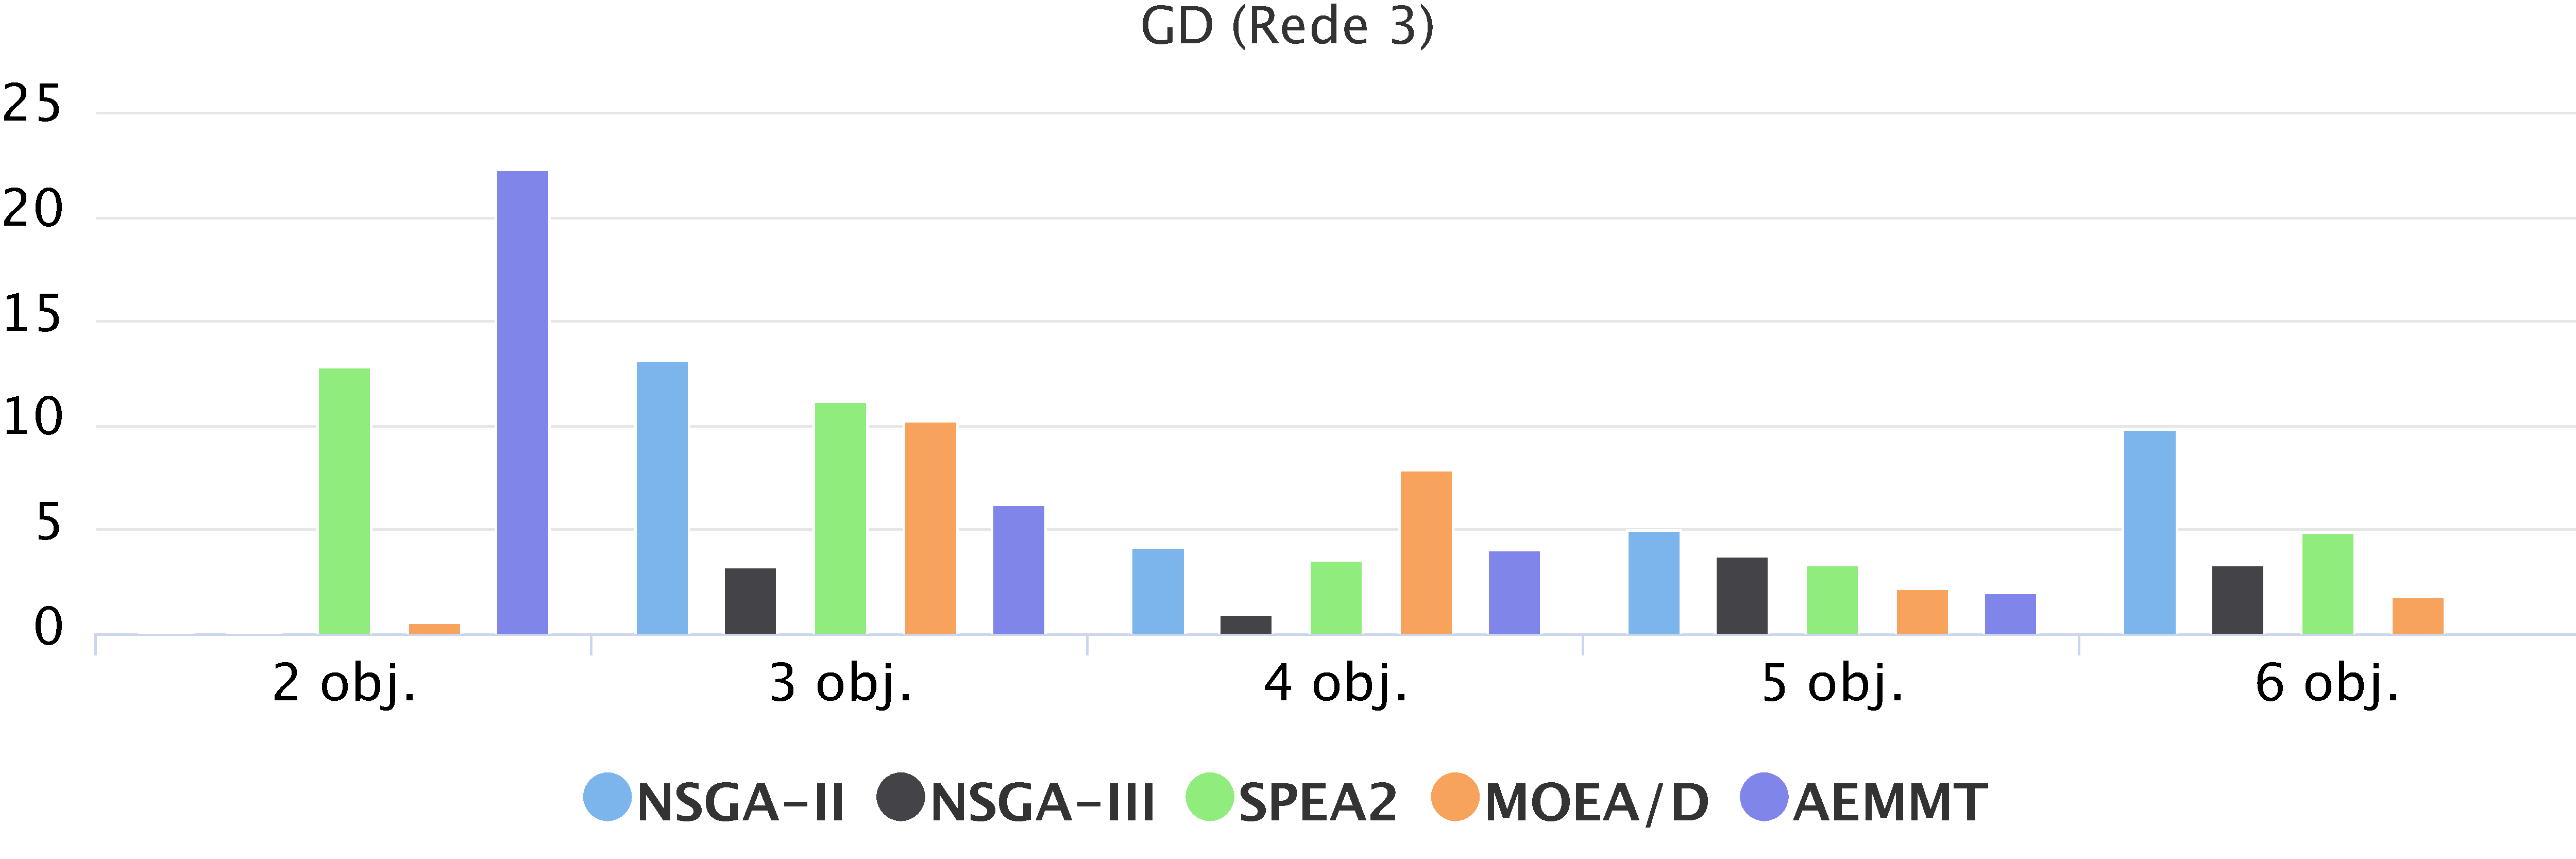
\includegraphics[width=1\textwidth]{cap_experimentos/figs/etapa1/gd-mrp-r3}
	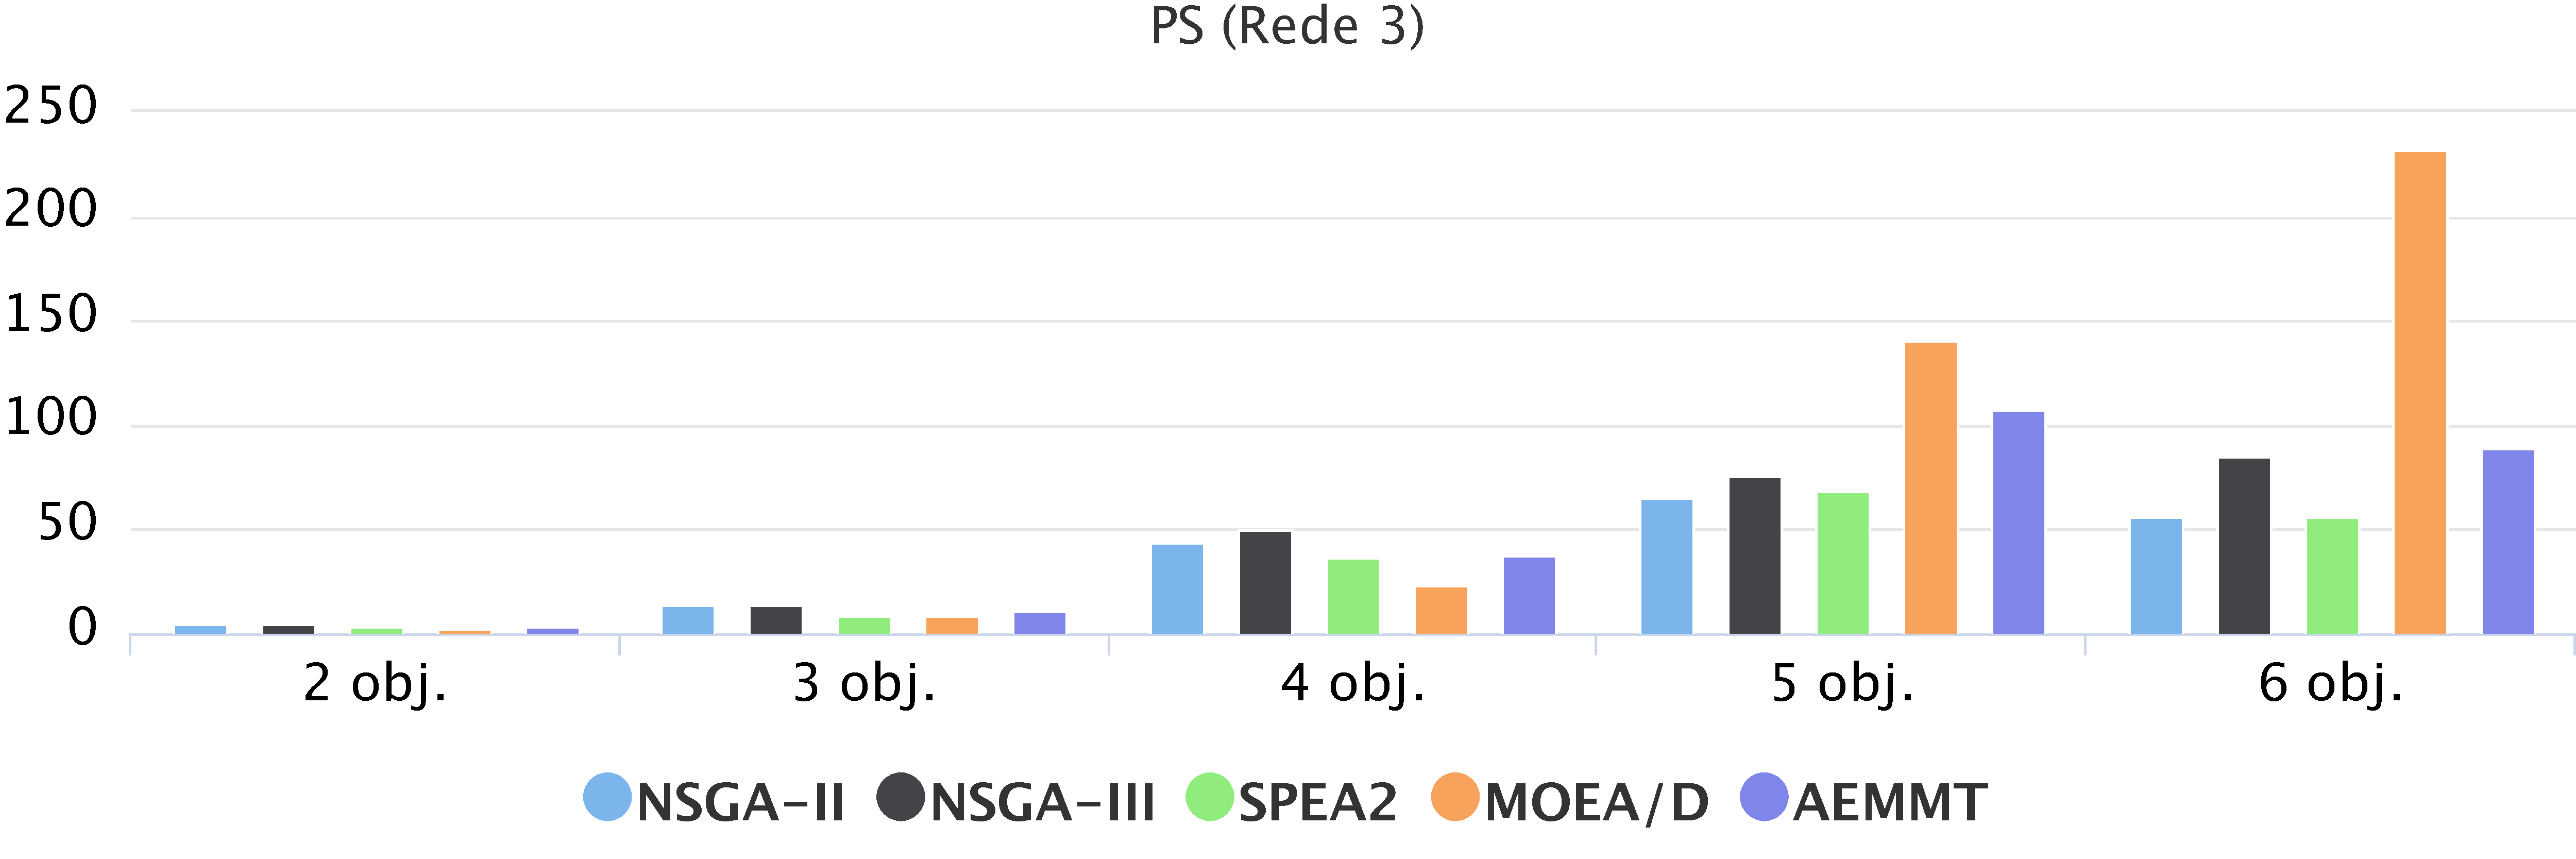
\includegraphics[width=1\textwidth]{cap_experimentos/figs/etapa1/ps-mrp-r3}
	\caption{\label{fig_exp1_prm_r3}Desempenho dos algoritmos na 1ª etapa para o PRM na rede 3}
\end{figure*}

A rede 3 é a mais complexa analisada nesta etapa dos experimentos. Analisando os resultados dos gráficos apresentados na \autoref{fig_exp1_prm_r3}, a tendência já observada nas demais instâncias é mantida, na qual o NSGA-III continua sendo o melhor método para as formulações com poucos objetivos. Até 4 objetivos, em todas as métricas, o NSGA-III apresenta os melhores resultados. Para 5 e 6 objetivos, o AEMMT apresenta menor $ER$ e $GD$, enquanto o MOEA/D consegue maior $PS$.

\begin{figure*}[!htbp]	
	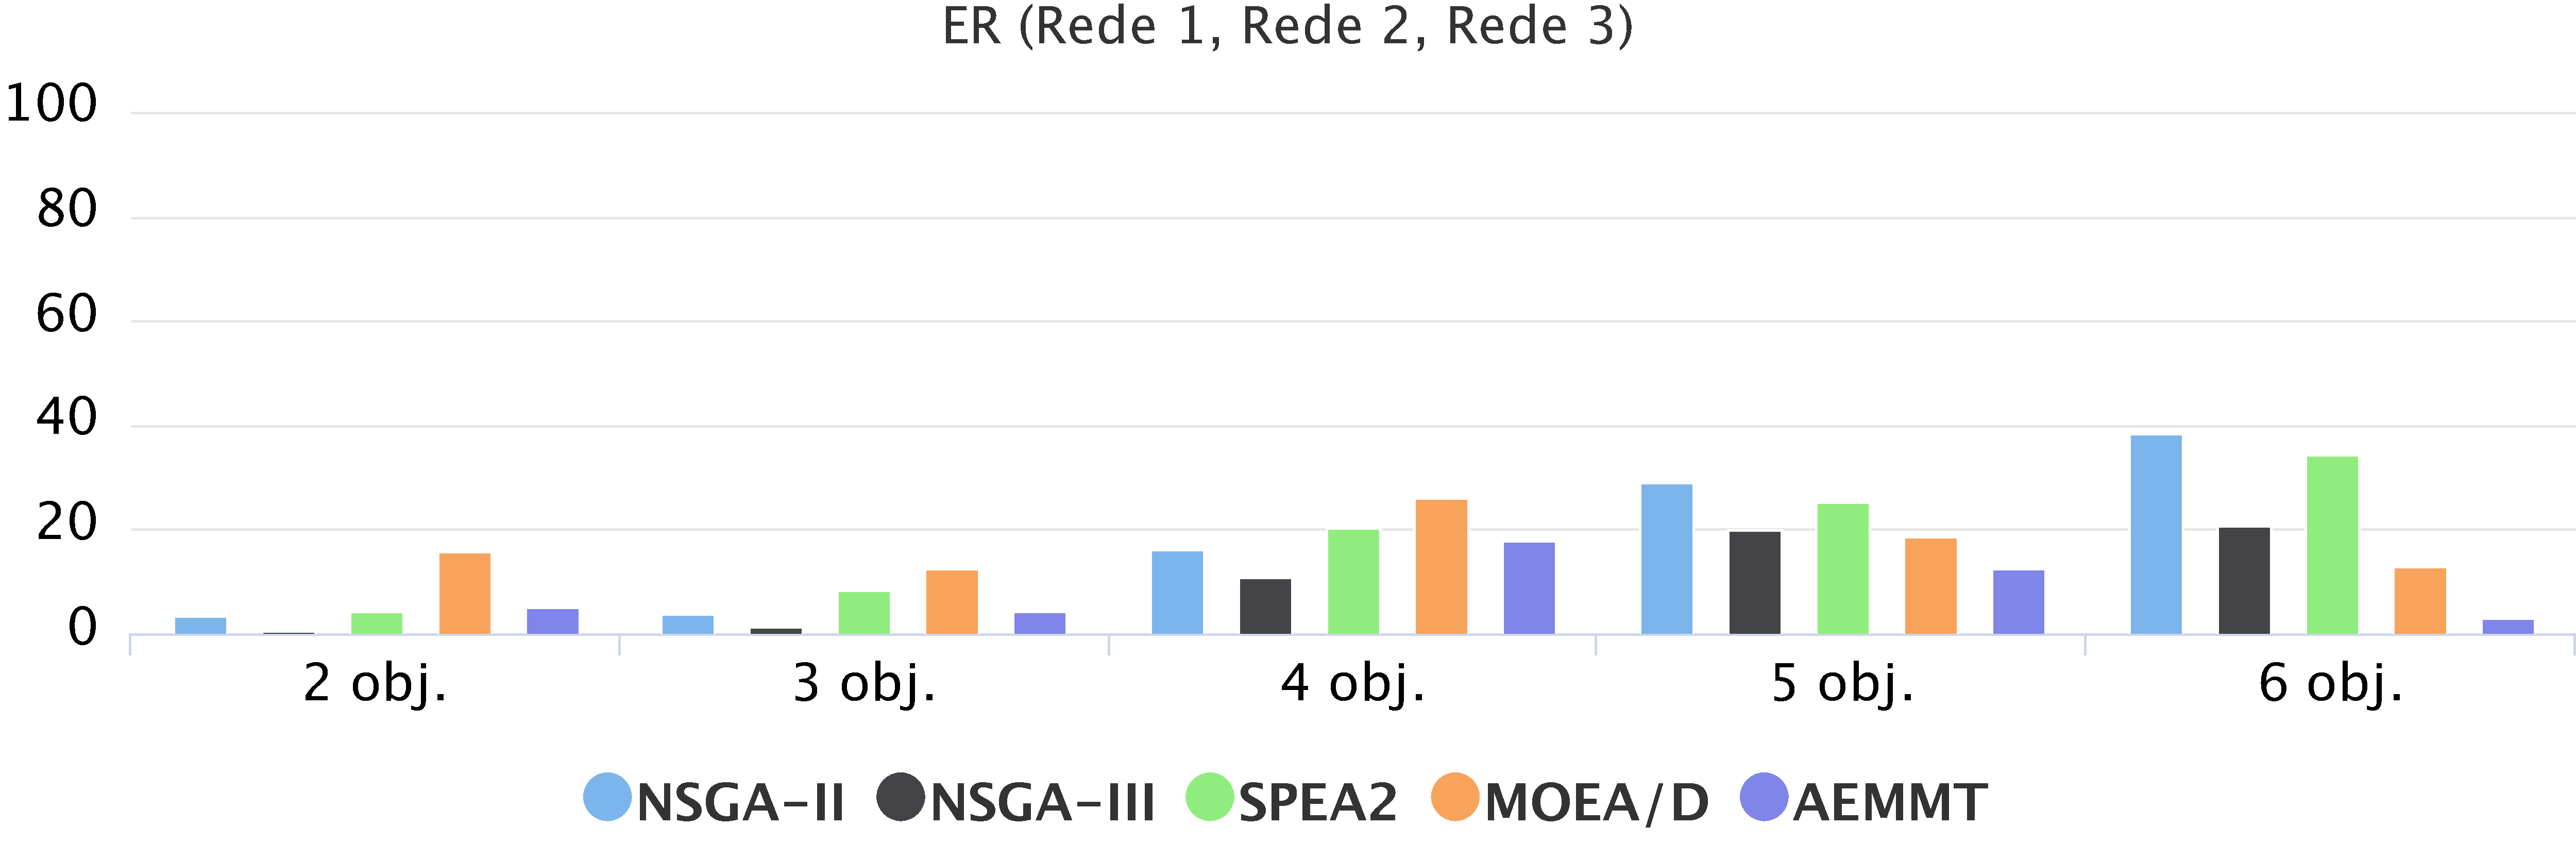
\includegraphics[width=1\textwidth]{cap_experimentos/figs/etapa1/er-mrp-todos}
	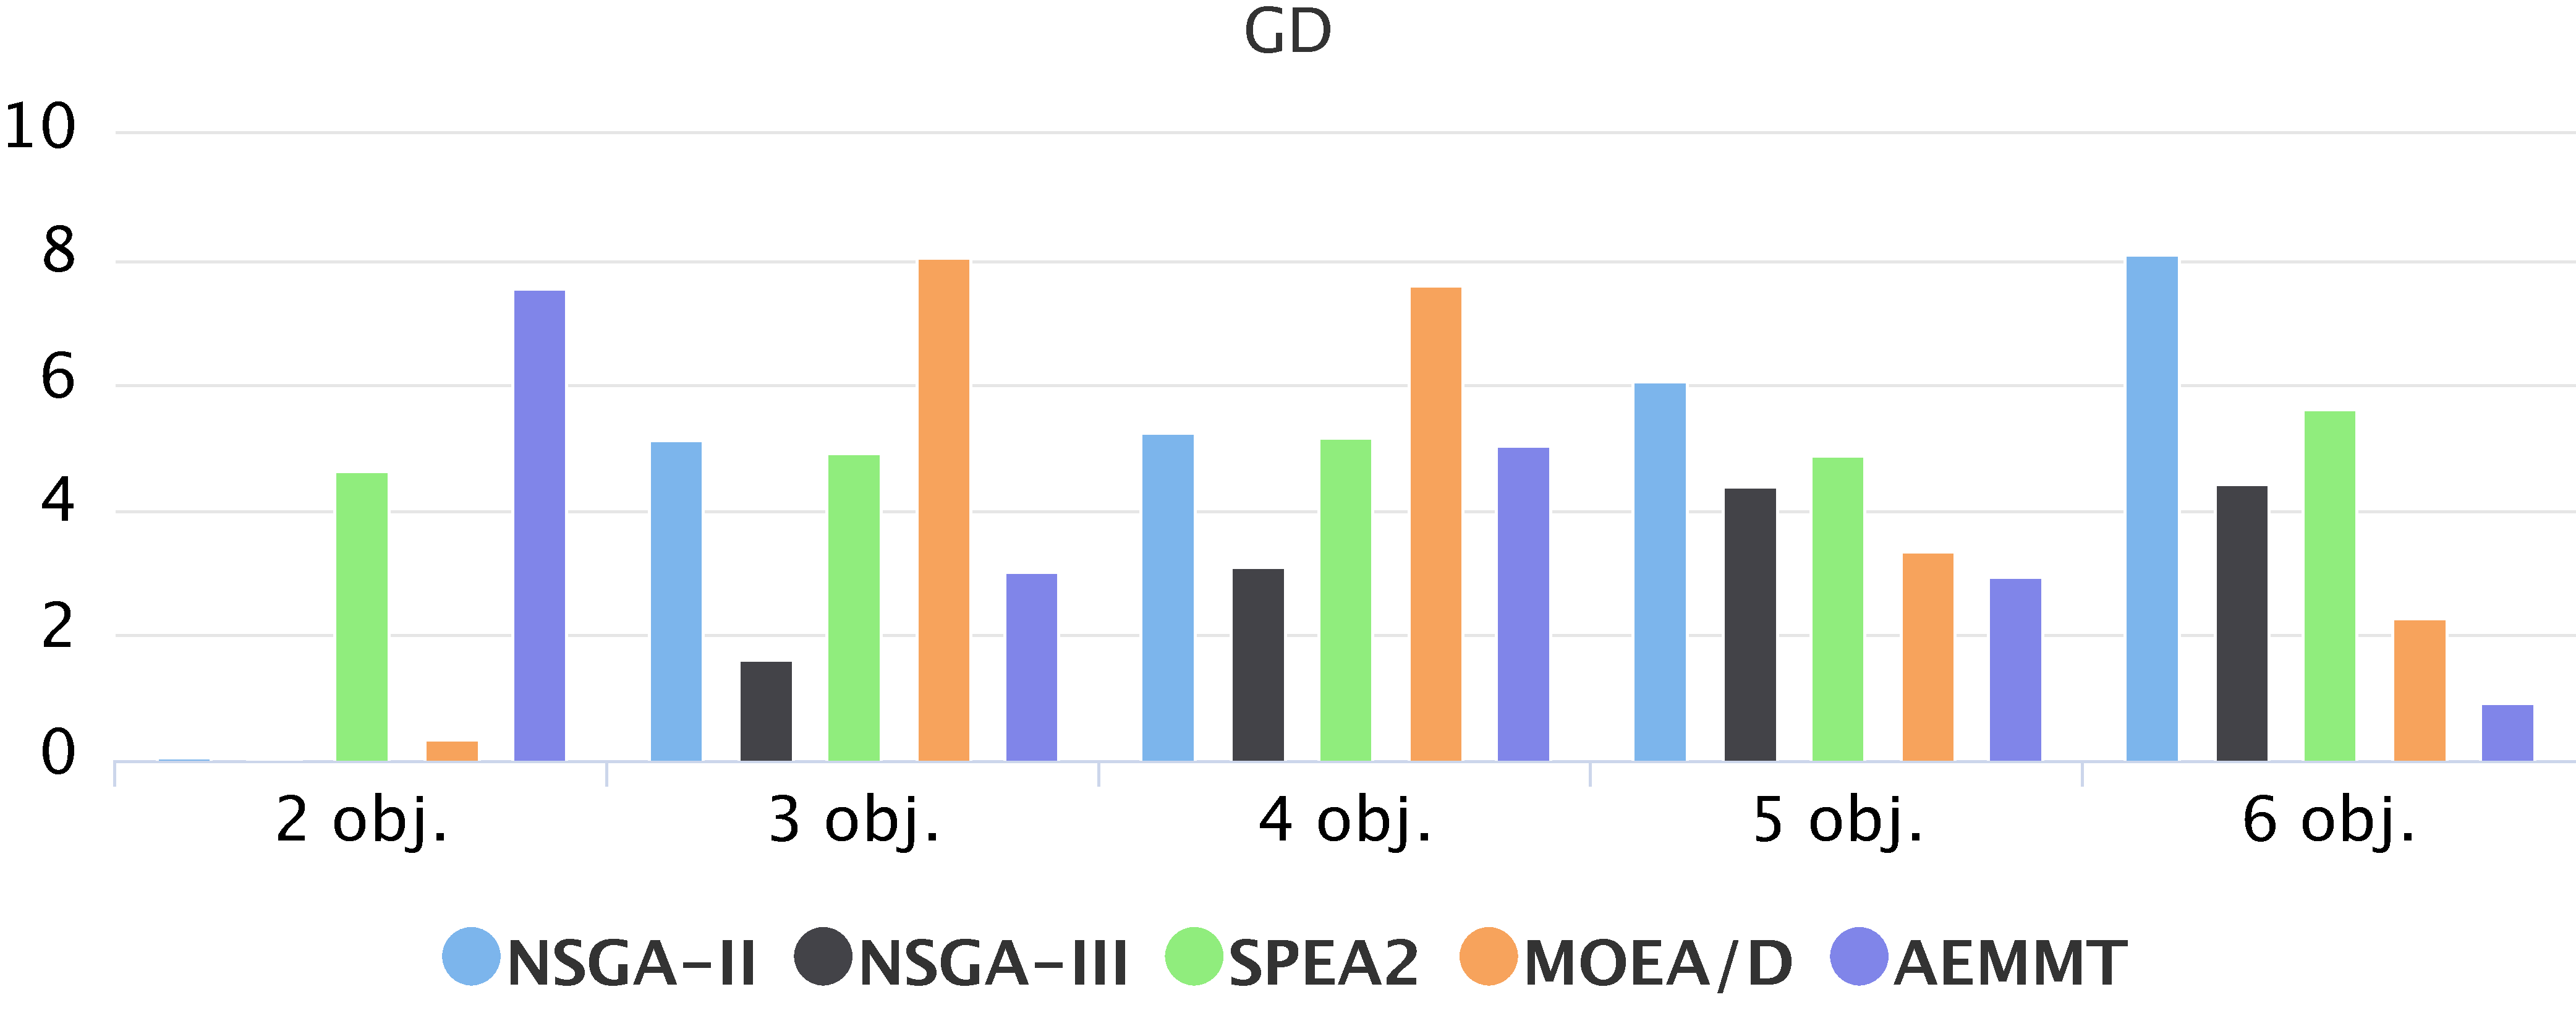
\includegraphics[width=1\textwidth]{cap_experimentos/figs/etapa1/gd-mrp-todos}
	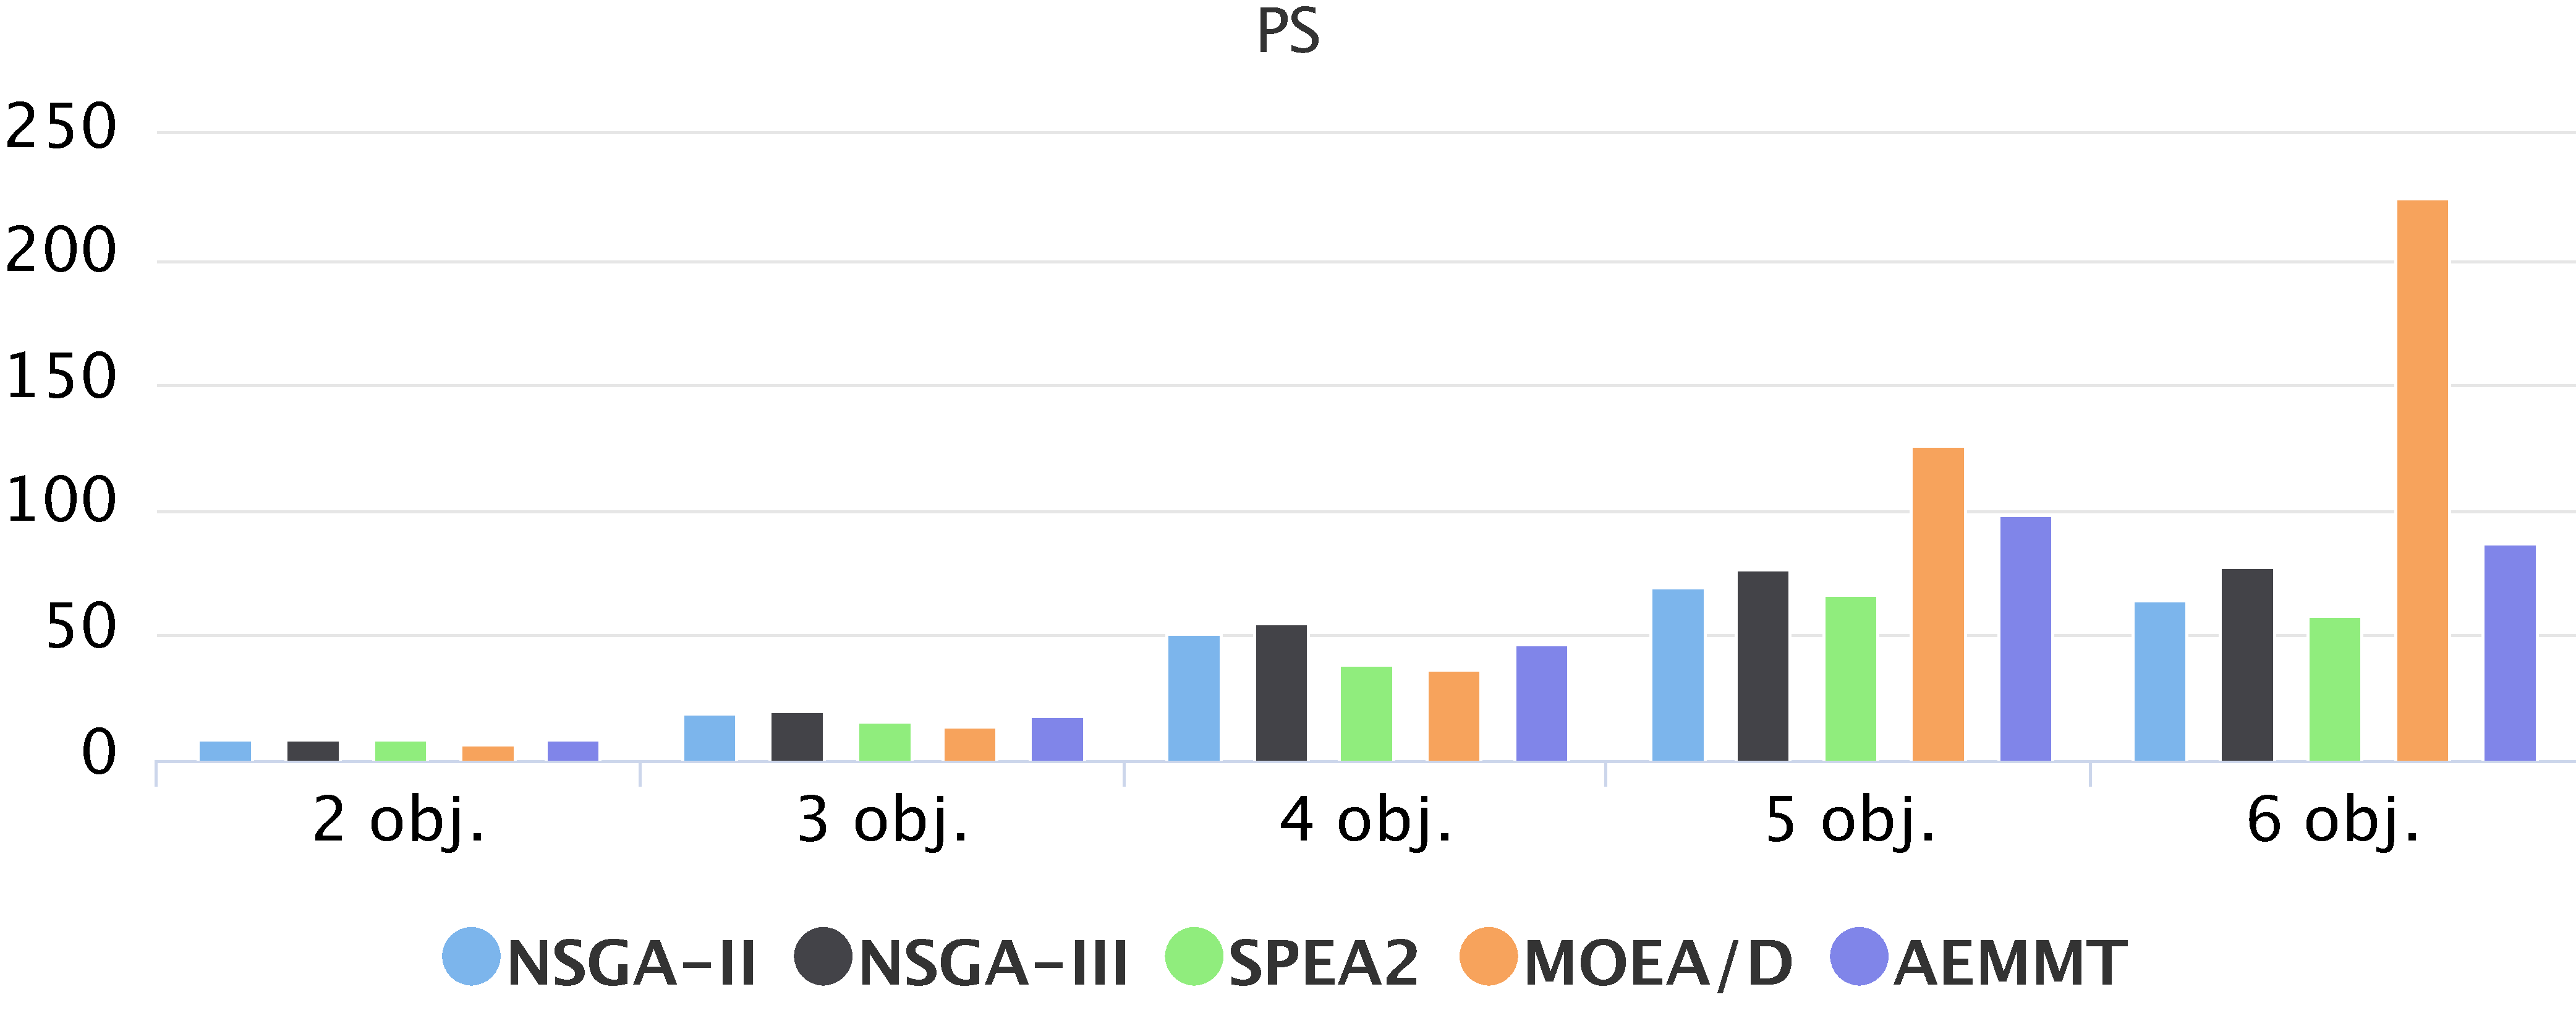
\includegraphics[width=1\textwidth]{cap_experimentos/figs/etapa1/ps-mrp-todos}
	\caption{\label{fig_exp1_prm_todos}Resultado consolidado da 1ª etapa considerando o PRM nas redes 1, 2, e 3}
\end{figure*}

A fim de fazer uma análise geral do PRM, os desempenhos dos algoritmos em todas as instâncias do problema (redes 1, 2 e 3) são consolidados nos gráficos da \autoref{fig_exp1_prm_todos}. Assim como no PMM, essa consolidação é obtida através da média aritmética dos valores das métricas em cada instância. Apesar de ser esperado que o NSGA-II e o SPEA2 fossem os melhores métodos para poucos objetivos, a partir dos gráficos da \autoref{fig_exp1_prm_todos}, observa-se que o NSGA-III obteve o melhor resultado para as formulações com 2, 3 e 4 objetivos. O NSGA-II também atinge bons resultados para 2 e 3 objetivos, mas o SPEA2 apresenta um $GD$ relativamente ruim. Considerando problemas de 5 e 6 objetivos, a escolha do algoritmo depende do intuito da busca. Se a quantidade encontrada de soluções do Pareto for mais relevante, o MOEA/D é mais indicado. Por outro lado, se um menor erro é preferível, então o AEMMT é a melhor opção.

Considerando ambos os problemas, PMM e PRM, os algoritmos NSGA-II, SPEA2 e NSGA-III são os que geram melhores resultados para problemas com poucos objetivos. O desempenho dos algoritmos clássicos (NSGA-II e SPEA2) diminui consideravelmente a medida que se aumenta o número de objetivos. Em contrapartida, o desempenho dos métodos AEMMT e MOEA/D melhora a partir de quatro objetivos, tornando-os mais indicados para problemas \textit{many-objectives}.

Outra observação que pôde ser feita a partir dos experimentos desta etapa é que o AEMMT perde apenas em $PS$ para o MOEA/D. Uma das características do AEMMT é a limitação no tamanho do arquivo, o que levanta a seguinte questão: se não houvesse esse limite, o AEMMT alcançaria melhor resultado em todas as métricas? Visando responder tal questão,foram executados novos experimentos para avaliar o desempenho de uma variação do AEMMT (AEMMT-F), na qual não existe um limite para o tamanho do arquivo. Na maioria dos experimentos, o AEMMT-F apresentou uma taxa de erro maior que sua versão original. Em contrapartida, essa variação alcançou valores médios para as métricas $ER$ e $PS$ melhores que aqueles obtidos pelo MOEA/D, principalmente para as formulações com 5 e 6 objetivos (\textit{many-objective}). Essa superioridade foi confirmada através de um teste de hipótese paramétrico, chamado de teste Z (\textit{Z-test}) com 0,1\% de significância ($\alpha = 0,1$).

Todos os experimentos apresentados nesta seção serviram como base para a elaboração de um artigo publicado no \ac{BRACIS} \cite{Franca2017}.

\section{Análise das estratégias e configurações para o MACO/NDS}
\label{section_experimentos_etapa2}

Com um novo algoritmo ACO em mente, o MACO/NDS, fez-se necessário um estudo sobre os métodos para a construção das soluções no PRM. Além disso, foi também preciso testar modelos de atualização de feromônio e ideias sobre os parâmetros de entrada $\alpha$ e $\beta$ do algoritmo. A fim de propor o novo método de otimização \textit{many-objective} e um modelo de aplicação para o PRM, realizou-se a segunda etapa de experimentos, onde várias configurações possíveis do algoritmo e do modelo foram testadas.

Inicialmente, um modelo de construção das soluções do PRM no MACO/NDS foi concebido de acordo com os experimentos realizados nesta etapa. O mesmo processo não foi realizado para o PMM, pois o modelo descrito em \cite{Alaya2004} já funciona bem para o MACO/D quando aplicado junto à técnica de amostragem (Seção \ref{section_algoritmo_pmm}). Além disso, nesses experimentos também avaliou-se diferentes aspectos sobre a atualização de feromônios e parâmetros de entrada no ACO, resultando em particularidades do algoritmo proposto.

Os experimentos dessa etapa foram realizados em duas fases. A primeira investiga o impacto de diferentes modelos de construção das soluções no desempenho do algoritmo proposto. Nesses experimentos, optou-se por simplificar o problema investigado a partir da adoção de um cenário com um único objetivo (mono-objetivo), possibilitando a avaliação, de maneira isolada, do processo de construção das soluções. Os experimentos da segunda fase visam analisar a influência de mudanças nas estratégias e configurações adotadas pelo MACO/NDS para resolver problemas multiobjetivos. Essas mudanças envolvem a construção de soluções por amostragem, formas de depósito de feromônio e dinamização dos parâmetros de entrada. Maiores detalhes sobre os experimentos de cada fase são dados a seguir.

Nos experimentos com o problema mono-objetivo, foram avaliadas quatro estratégias (descritas na Seção \ref{section_algoritmo_prm}):

\begin{enumerate}
	\item Formiga única: o espaço de busca é explorado de forma aleatória, mas sempre considerando apenas a vizinhança da posição atual da formiga.
	\item Múltiplas formigas: uma formiga para cada destino. Une-se os caminhos produzidos por cada agente em uma árvore.
	\item Formiga com sobreposição: uma formiga explora o espaço de busca de forma aleatória, podendo estar em vários nós ao mesmo tempo. Essa estratégia elimina o problema de localidade na busca.
	\item Formigas invertidas: uma formiga para cada destino, mas ao invés construírem uma trajetória da raiz ao destino, fazem o caminho contrário, ou seja, partem do destino e tentam encontrar a raiz.
\end{enumerate}

O problema mono-objetivo criado consiste em minimizar o valor do produto entre custo e atraso ($f(x) = custo(x) \times delay(x)$) de uma árvore. Portanto, quanto menor esse valor, melhor a árvore obtida. Além das quatro estratégias avaliadas, também foi implementada uma modificação do algoritmo de Prim \cite{Prim1957} para servir como referência de uma solução potencial para o PRM. Cada estratégia foi executada cinco vezes e a tabela \ref{tab_exp2_estrategias} mostra o resultado da melhor execução de cada estratégia. Nessa tabela, a coluna ``resultado'' representa a soma dos valores de $custo \times delay$ das arestas da árvore obtida como solução, ou seja, quanto menor esse valor, melhor a solução obtida.

\begin{table}[!htbp]
	\centering
	\caption{Desempenho em função da estratégia de construção de uma solução para o PRM}
	\label{tab_exp2_estrategias}
	\begin{tabular}{rrrr}
		Estratégia & Rede & Resultado   & Tempo (s)    \\ \hline
		Prim       & $R_1$   & 3.28 & 0.02     \\
		1          & $R_1$   & 3.04 & 2.49     \\
		2          & $R_1$   & 3.03 & 5.94      \\
		\rowcolor{table-green} 
		3          & $R_1$   & 3.00 & 3.88      \\
		\rowcolor{table-green} 
		4          & $R_1$   & 3.00 & 3.16      \\ \hline
		Prim       & $R_2$   & 3.13 & 0.01     \\
		1          & $R_2$   & 3.34 & 4.94     \\
		2          & $R_2$   & 3.26 & 13.22     \\
		\rowcolor{table-green} 
		3          & $R_2$   & 3.13 & 10.69    \\
		4          & $R_2$   & 3.30 & 5.549     \\ \hline
		Prim       & $R_3$   & 7.96 & 0.024     \\
		1          & $R_3$   & 8.13 & 4.212     \\
		2          & $R_3$   & 8.23 & 25.60    \\
		\rowcolor{table-green} 
		3          & $R_3$   & 7.48 & 9.82     \\
		4          & $R_3$   & 8.11 & 6.93     \\ \hline
		Prim       & $R_4$   & 1.80 & 0.02     \\
		1          & $R_4$   & 2.34 & 4.71     \\
		2          & $R_4$   & 2.32 & 12.47    \\
		\rowcolor{table-green} 
		3          & $R_4$   & 1.85 & 11.01    \\
		4          & $R_4$   & 1.97 & 4.93     \\ \hline
		Prim       & $R_5$   & 6.34 & 0.01     \\
		1          & $R_5$   & 6.12 & 6.87      \\
		2          & $R_5$   & 6.33 & 17.38     \\
		\rowcolor{table-green} 
		3          & $R_5$   & 5.85 & 14.76    \\
		\rowcolor{table-green} 
		4          & $R_5$   & 5.85 & 8.42     \\ \hline
	\end{tabular}
\end{table}

Como pode ser observado na tabela, a estratégia número 3, que usa a ideia de formiga com super-posição, obteve o melhor valor para a função objetivo (resultado). Em contrapartida, ela foi a segunda pior estratégia em relação ao tempo. Por essa razão, propõe-se a ideia de amostragem explicada na Seção \ref{section_algoritmo_prm}. Ao invés de se utilizar todo o conjunto de exploração, a construção da solução é realizada sobre uma amostra dele. Em nossos experimentos para o PRM, a amostragem é de 10 elementos. A Tabela \ref{tab_exp2_amostragem} mostra uma comparação dos melhores valores obtidos utilizando a estratégia 3, com e sem essa amostragem.

\begin{table}[!htbp]
	\centering
	\caption{Resultados obtidos a partir da estratégia 3 de acordo com o espaço de exploração considerado (com e sem amostragem)}
	\label{tab_exp2_amostragem}
	\begin{tabular}{rrrr}
		Amostragem    & Rede & Resultado   & Tempo (s) \\ \hline
		s/ amostragem & $R_1$    & 3.007936508 & 3.88      \\
		\rowcolor{table-green}
		c/ amostragem & $R_1$    & 3.007936508 & 3.41      \\ \hline
		s/ amostragem & $R_2$    & 3.134920635 & 10.694    \\
		\rowcolor{table-green}
		c/ amostragem & $R_2$    & 3.134920635 & 7.602     \\ \hline
		s/ amostragem & $R_3$    & 7.484126984 & 9.821     \\
		\rowcolor{table-green}
		c/ amostragem & $R_3$    & 7.484126984 & 7.26      \\ \hline
		s/ amostragem & $R_4$    & 1.857142857 & 11.015    \\
		\rowcolor{table-green}
		c/ amostragem & $R_4$    & 1.785714286 & 7.28      \\ \hline
		s/ amostragem & $R_5$    & 5.857142857 & 14.767    \\
		\rowcolor{table-green}
		c/ amostragem & $R_5$    & 5.76984127  & 10.037    \\ \hline
	\end{tabular}
\end{table}

Como pode ser observado na Tabela \ref{tab_exp2_amostragem}, a amostragem não só diminuiu o tempo do algoritmo como também melhorou o resultado para as redes mais complexas ($R_5$ e $R_6$). A melhora na qualidade da solução pode ser atribuída ao maior grau de aleatoriedade dada ao algoritmo, similar ao que acontece nos algoritmos genéticos quando se lança mão de operações como a mutação ou seleções por torneio.

Ao implementar a estratégia 3 (uma formiga com super-posição) com amostragem no PRM \textit{many-objetive}, percebeu-se que o AEMMD atinge um desempenho muito superior ao do novo algoritmo, como apresentado na Tabela \ref{tab_exp2_macod_simples}. A fim de reduzir essa diferença, propôs-se as seguintes mudanças para o MACO/NDS:

\begin{itemize}
	\item Depósito de feromônio baseado na qualidade da aresta (ou do item, no caso do PMM): em um problema multiobjetivo, ao depositar feromônios sobre as arestas correspondentes às soluções não-dominadas, normalmente é utilizada a mesma quantidade independente da solução e da aresta. Isso ocorre porque, segundo a relação de não-dominância, ambas opções são igualmente boas. Entretanto, nossa nova estratégia muda esse conceito, relacionando a quantidade de feromônios depositada à qualidade da aresta. Nesse contexto, considerando que é um problema de minimização, a quantidade passa a ser inversamente proporcional à soma dos pesos da aresta.
	\item Dinamização do parâmetro de entrada $\beta$: esse parâmetro controla a importância da heurística no cálculo das probabilidades de cada aresta (ou item, no PMM) fazer parte da solução. Nossa proposta é diminuir um pouco a importância da heurística, dando maior peso à informação de feromônio sempre que, após uma iteração, não for encontrada uma nova solução. Esse processo se repete a cada iteração até que uma nova solução é encontrada, o valor de $\beta$ é reiniciado para o padrão (fornecido como entrada para o algoritmo).
\end{itemize}

Considerando a formulação do PRM com seis objetivos, a Tabela \ref{tab_exp2_macod_simples} mostra as diferenças entre os desempenhos dos algoritmos AEMMD, MACO/NDS antes das alterações no depósito de feromônios e do parâmetro $\beta$ (MACO/NDS-pré) e do algoritmo final proposto no capítulo \ref{chapter_macod} (MACO/NDS). Essa comparação é feita com base nos valores médios das métricas de desempenho multiobjetivo ($ER$, $GD$ e $PS$).

\begin{table}[!htbp]
	\centering
	\caption{Análise comparativa entre as implementações do MACO/NDS e o AEMMD no PRM multiobjetivo}
	\label{tab_exp2_macod_simples}
	\begin{tabular}{rrrrr}
		Algoritmo  & Rede  & $ER$  & $GD$ & $PS$  \\ \hline
		AEMMD      & $R_1$ & 6.59  & 0.38 & 502.8 \\
		MACO/NDS-pré & $R_1$ & 18.42 & 0.30 & 337.6 \\
		MACO/NDS     & $R_1$ & 11.57 & 0.36 & 424.2 \\ \hline
		AEMMD      & $R_2$ & 7.58  & 0.49 & 296.6 \\
		MACO/NDS-pré & $R_2$ & 11.75 & 0.47 & 284.4 \\
		MACO/NDS     & $R_2$ & 11.18 & 0.37 & 300   \\ \hline
		AEMMD      & $R_3$ & 11.73 & 0.19 & 388.6 \\
		MACO/NDS-pré & $R_3$ & 36.47 & 0.16 & 206   \\
		MACO/NDS     & $R_3$ & 30.20 & 0.25 & 232.4 \\ \hline
		AEMMD      & $R_4$ & 35.88 & 0.17 & 234   \\
		MACO/NDS-pré & $R_4$ & 54.48 & 0.11 & 150.2 \\
		MACO/NDS     & $R_4$ & 50.57 & 0.15 & 186.6 \\ \hline
		AEMMD      & $R_5$ & 32.67 & 0.20 & 181.2 \\
		MACO/NDS-pré & $R_5$ & 32.95 & 0.22 & 168.6 \\
		MACO/NDS     & $R_5$ & 32.67 & 0.30 & 160.8
	\end{tabular}
\end{table}

Na Tabela \ref{tab_exp2_macod_simples} pode-se observar que, na maioria dos casos, as duas alterações propostas melhoraram o resultado do MACO/NDS nas métricas ER e PS (nas quais o AEMMD é superior). Portanto, o algoritmo final proposto inclui essas duas alterações. Apesar do AEMMD ainda apresentar melhores resultados de desempenho, a nova versão do algoritmo conseguiu reduzir a diferença nas métricas $ER$ e $PS$.

\section{Análise comparativa entre o MACO/NDSD e os AEMOs \textit{many-objective}}
\label{section_experimentos_etapa3}

Na terceira etapa, os experimentos visam avaliar a eficiência dos métodos de otimização \textit{many-objective} NSGA-III, MOEA/D, AEMMT, AEMMD, MOACS, MOEA/D-ACO e do algoritmo proposto, MACO/NDS, nos problemas da mochila e do roteamento multicast. Nessa etapa são testadas formulações com 4, 5 e 6 objetivos, avaliando-se 3 redes no PRM e problemas com 30, 40 e 50 itens no PMM. Os experimentos colocam à prova pela primeira vez o algoritmo proposto neste trabalho e revelam suas vantagens e fraquezas, possibilitando a identificação dos cenários nos quais sua utilização é mais adequada e as formas de melhorá-lo em cenários onde os seus resultados foram desfavoráveis.

Por abordar apenas problemas com muitos objetivos (\textit{many-objective}), nesses experimentos foram descartados os AEMOs clássicos (NSGA-II e SPEA2) e incluídos os algoritmos AEMMD e o MACO/NDS (algoritmo proposto neste trabalho). Em todas as execuções, os algoritmos utilizaram os mesmos parâmetros de configuração, os quais estão descritos na Tabela \ref{table_exp3_parametros}. No caso do AEMMT e do AEMMD, o número de gerações (marcado com asterisco) deve ser multiplicado pelo tamanho da população. Esse ajuste visa equiparar a quantidade de soluções avaliadas, dado que esse algoritmos realizam apenas um \textit{crossover} por geração. Durante a análise dos resultados, foram empregadas todas as métricas de desempenho utilizadas nas etapas anteriores: erro ($ER$),  distância ($GD$) e número de soluções do Pareto encontradas ($PS$). Além dessas três métricas sobre o Pareto, mediu-se o tempo de execução do algoritmo (Tempo). Assim como na etapa 1, o Pareto aproximado foi pré-definido a partir de múltiplas execuções dos algoritmos. A quantidade de soluções pertencentes ao Pareto obtido para cada instância dos problemas investigados é apresentada na Tabela \ref{table_exp3_paretos}. A medida de tempo, como não pode ser obtida através da execução paralela dos algoritmos e necessita de exclusividade sobre a máquina, considerou a média de 3 execuções de cada algoritmo em cada cenário testado. As demais métricas foram obtidas através das médias entre 100 execuções dos 30 cenários na lista a seguir:

\begin{itemize}
	\item PRM: 3 formulações de objetivos ($P_4$, $P_5$ e $P_6$) e 3 redes ($R_1$, $R_2$ e $R_3$). Tanto as formulações quanto às redes foram descritas na Seção \ref{section_problemas_prm}.
	\item PMM: 3 formulações de objetivos (4 a 6) e 3 instâncias (30, 40 e 50 itens).
\end{itemize}


\begin{table}[!htbp]
	\centering
	\caption{Fronteira de Pareto estabelecida para os cenários investigados na 3ª etapa de experimentos}
	\label{table_exp3_paretos}
	\begin{tabular}{c|rrr|rrr}
		& \multicolumn{3}{c|}{\textbf{PRM}} & \multicolumn{3}{c}{\textbf{PMM}} \\ \hline
		Objetivos & R1         & R2       & R3        & 30 itens  & 40 itens & 50 itens \\ \hline
		4         & 122        & 553       & 1349        & 425       & 1199      & 1012    \\
		5         & 75        & 372      & 712       & 1769      & 3862     & 5467   \\
		6         & 60       & 660      & 1283      & 5828      & 6491   & 55471   \\ \hline
	\end{tabular}
\end{table}

\begin{table}[!htbp]
	\caption{Parâmetros utilizados pelos AEMOs na 3ª etapa, de acordo com o problema tratado}
	\label{table_exp3_parametros}
	\begin{center}
		\begin{tabular}{c|r|r}
			\textbf{Parâmetro} & \textbf{PRM} &  \textbf{PMM} \\ %\hline
			\hline
			Tamanho da população               &    90 &      150 \\ %\hline
			Número de gerações*        &   100 &      100 \\ %\hline
			Taxa de crossover                & 100\% &    100\% \\ %\hline
			Taxa de mutação                 &  20\% &      5\% \\ %\hline
			Tamanho da vizinhança (MOEA/D)    &    10 &       10 \\ %\hline
			Tamanho das tabelas (MEAMT)   &    30 &       50 \\ %\hline
			Tamanho da tabela de dominância (MEAMT) &    90 &      150 \\ %\hline
			Número de divisões (NSGA-III)&     8 &        8 \\ %\hline
			$\alpha, \beta, \rho$ (MACO/NDS)& 1, 2, 0.3 & 1, 4.3, 0.3 \\ %\hline
			Intervalo de valores para os feromônios (MACO/NDS)& [0.1, 0.9] & [0.1, 0.9] \\ %\hline
			Tamanho das amostras (MACO/NDS)& 10 &25\% do número de itens \\  %\hline
			Tamanho do grupo de estruturas ativas (MACO/NDS)& 5 & 5 \\
			\hline
		\end{tabular}
	\end{center}
\end{table}

As Figuras \ref{fig_exp3_pmm_30}, \ref{fig_exp3_pmm_40} e \ref{fig_exp3_pmm_50} mostram, respectivamente, o desempenho dos algoritmos para o PMM de 30, 40 e 50 itens. Já nas Figuras \ref{fig_exp3_prm_r1}, \ref{fig_exp3_prm_r2} e \ref{fig_exp3_prm_r3} são apresentados os resultados para o PRM considerando as $R_1$, $R_2$ e $R_3$, respectivamente. Uma análise consolidada, com a média entre as três instâncias de cada problema, é apresenta nas Figuras \ref{fig_exp3_pmm_todos} (PMM) e \ref{fig_exp3_prm_todos} (PRM).

\begin{figure*}[!htbp]	
	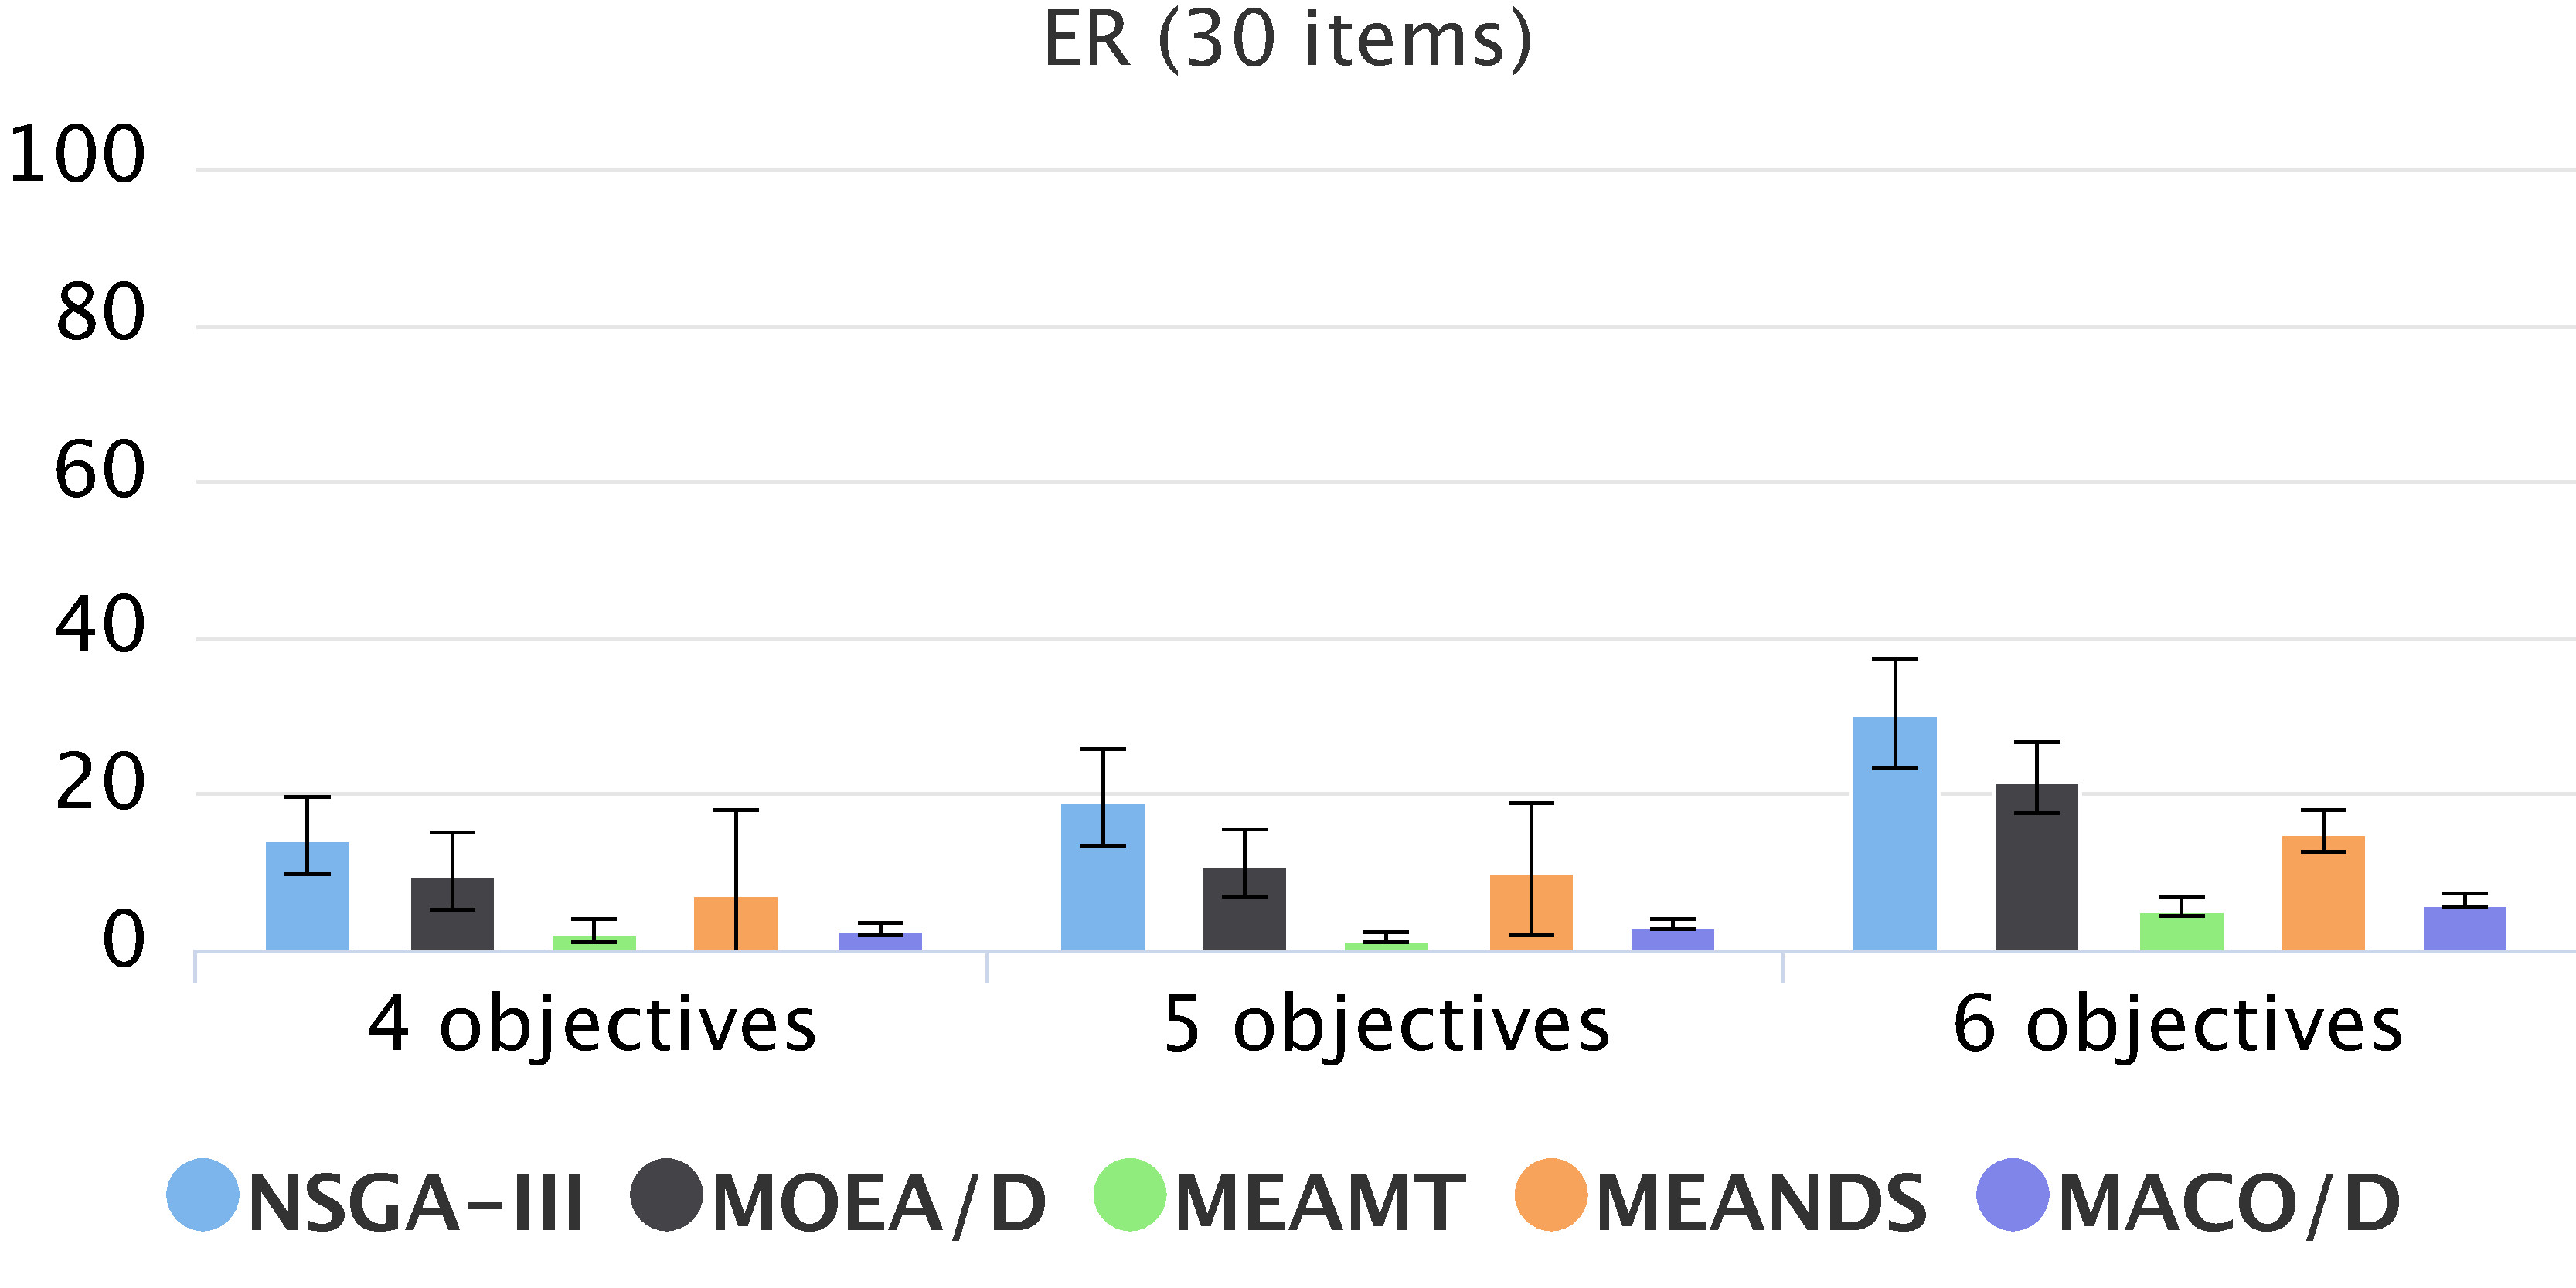
\includegraphics[width=0.5\textwidth]{cap_experimentos/figs/etapa3/er-mkp-30}
	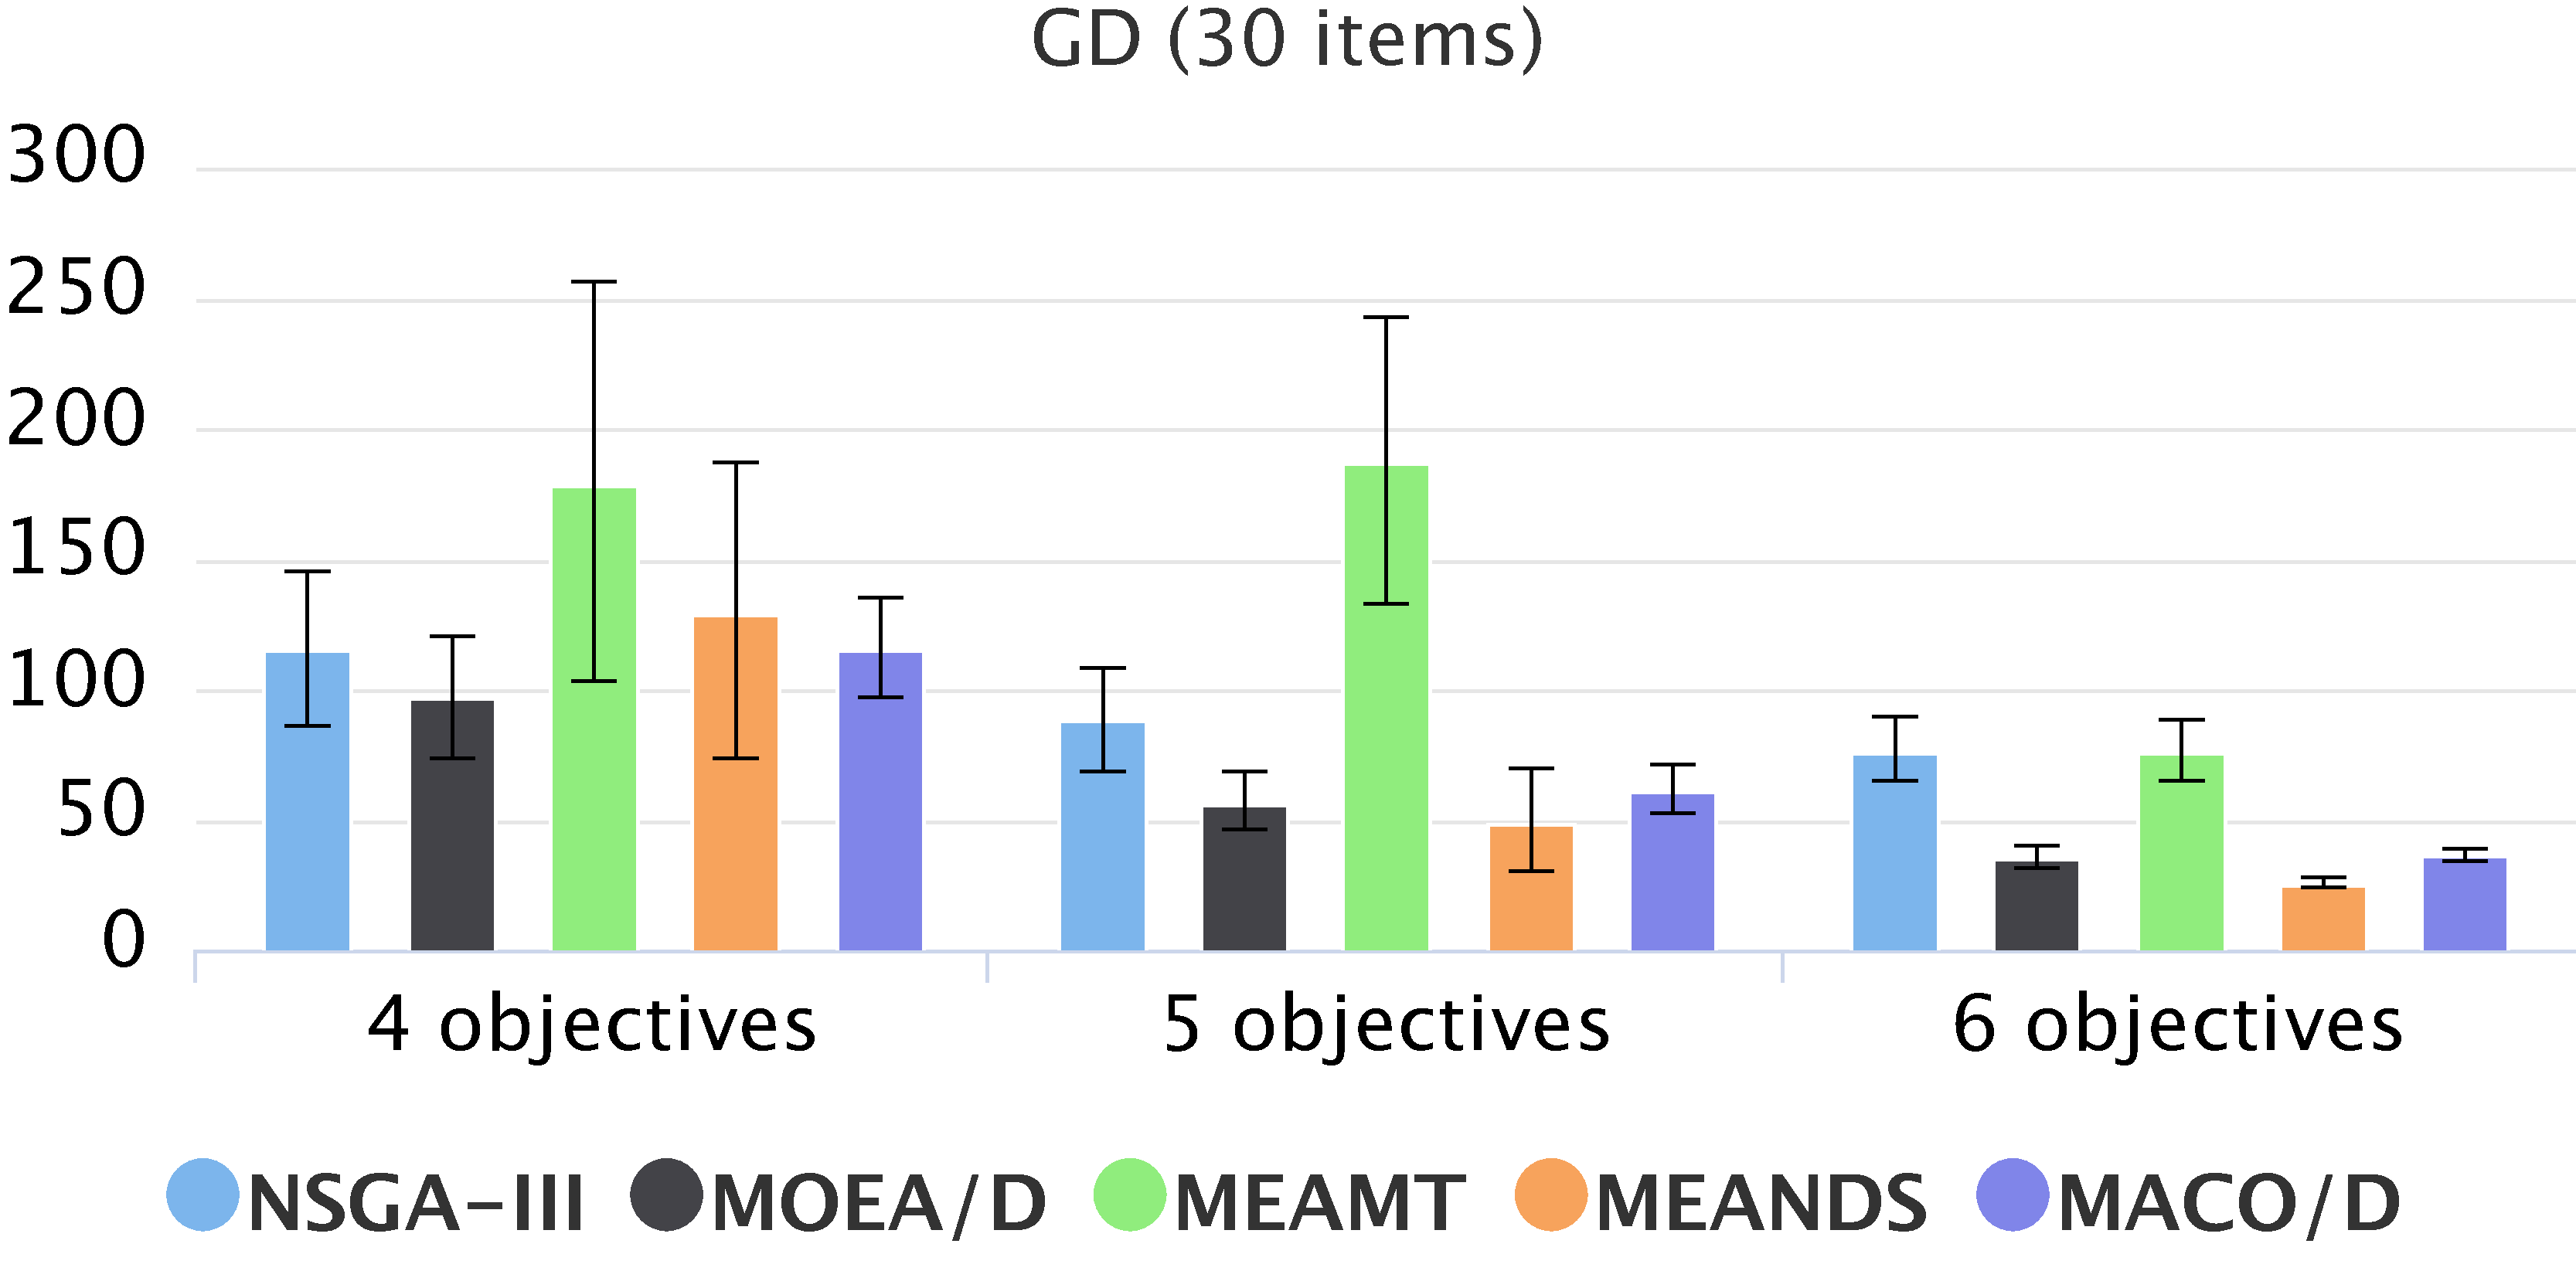
\includegraphics[width=0.5\textwidth]{cap_experimentos/figs/etapa3/gd-mkp-30}
	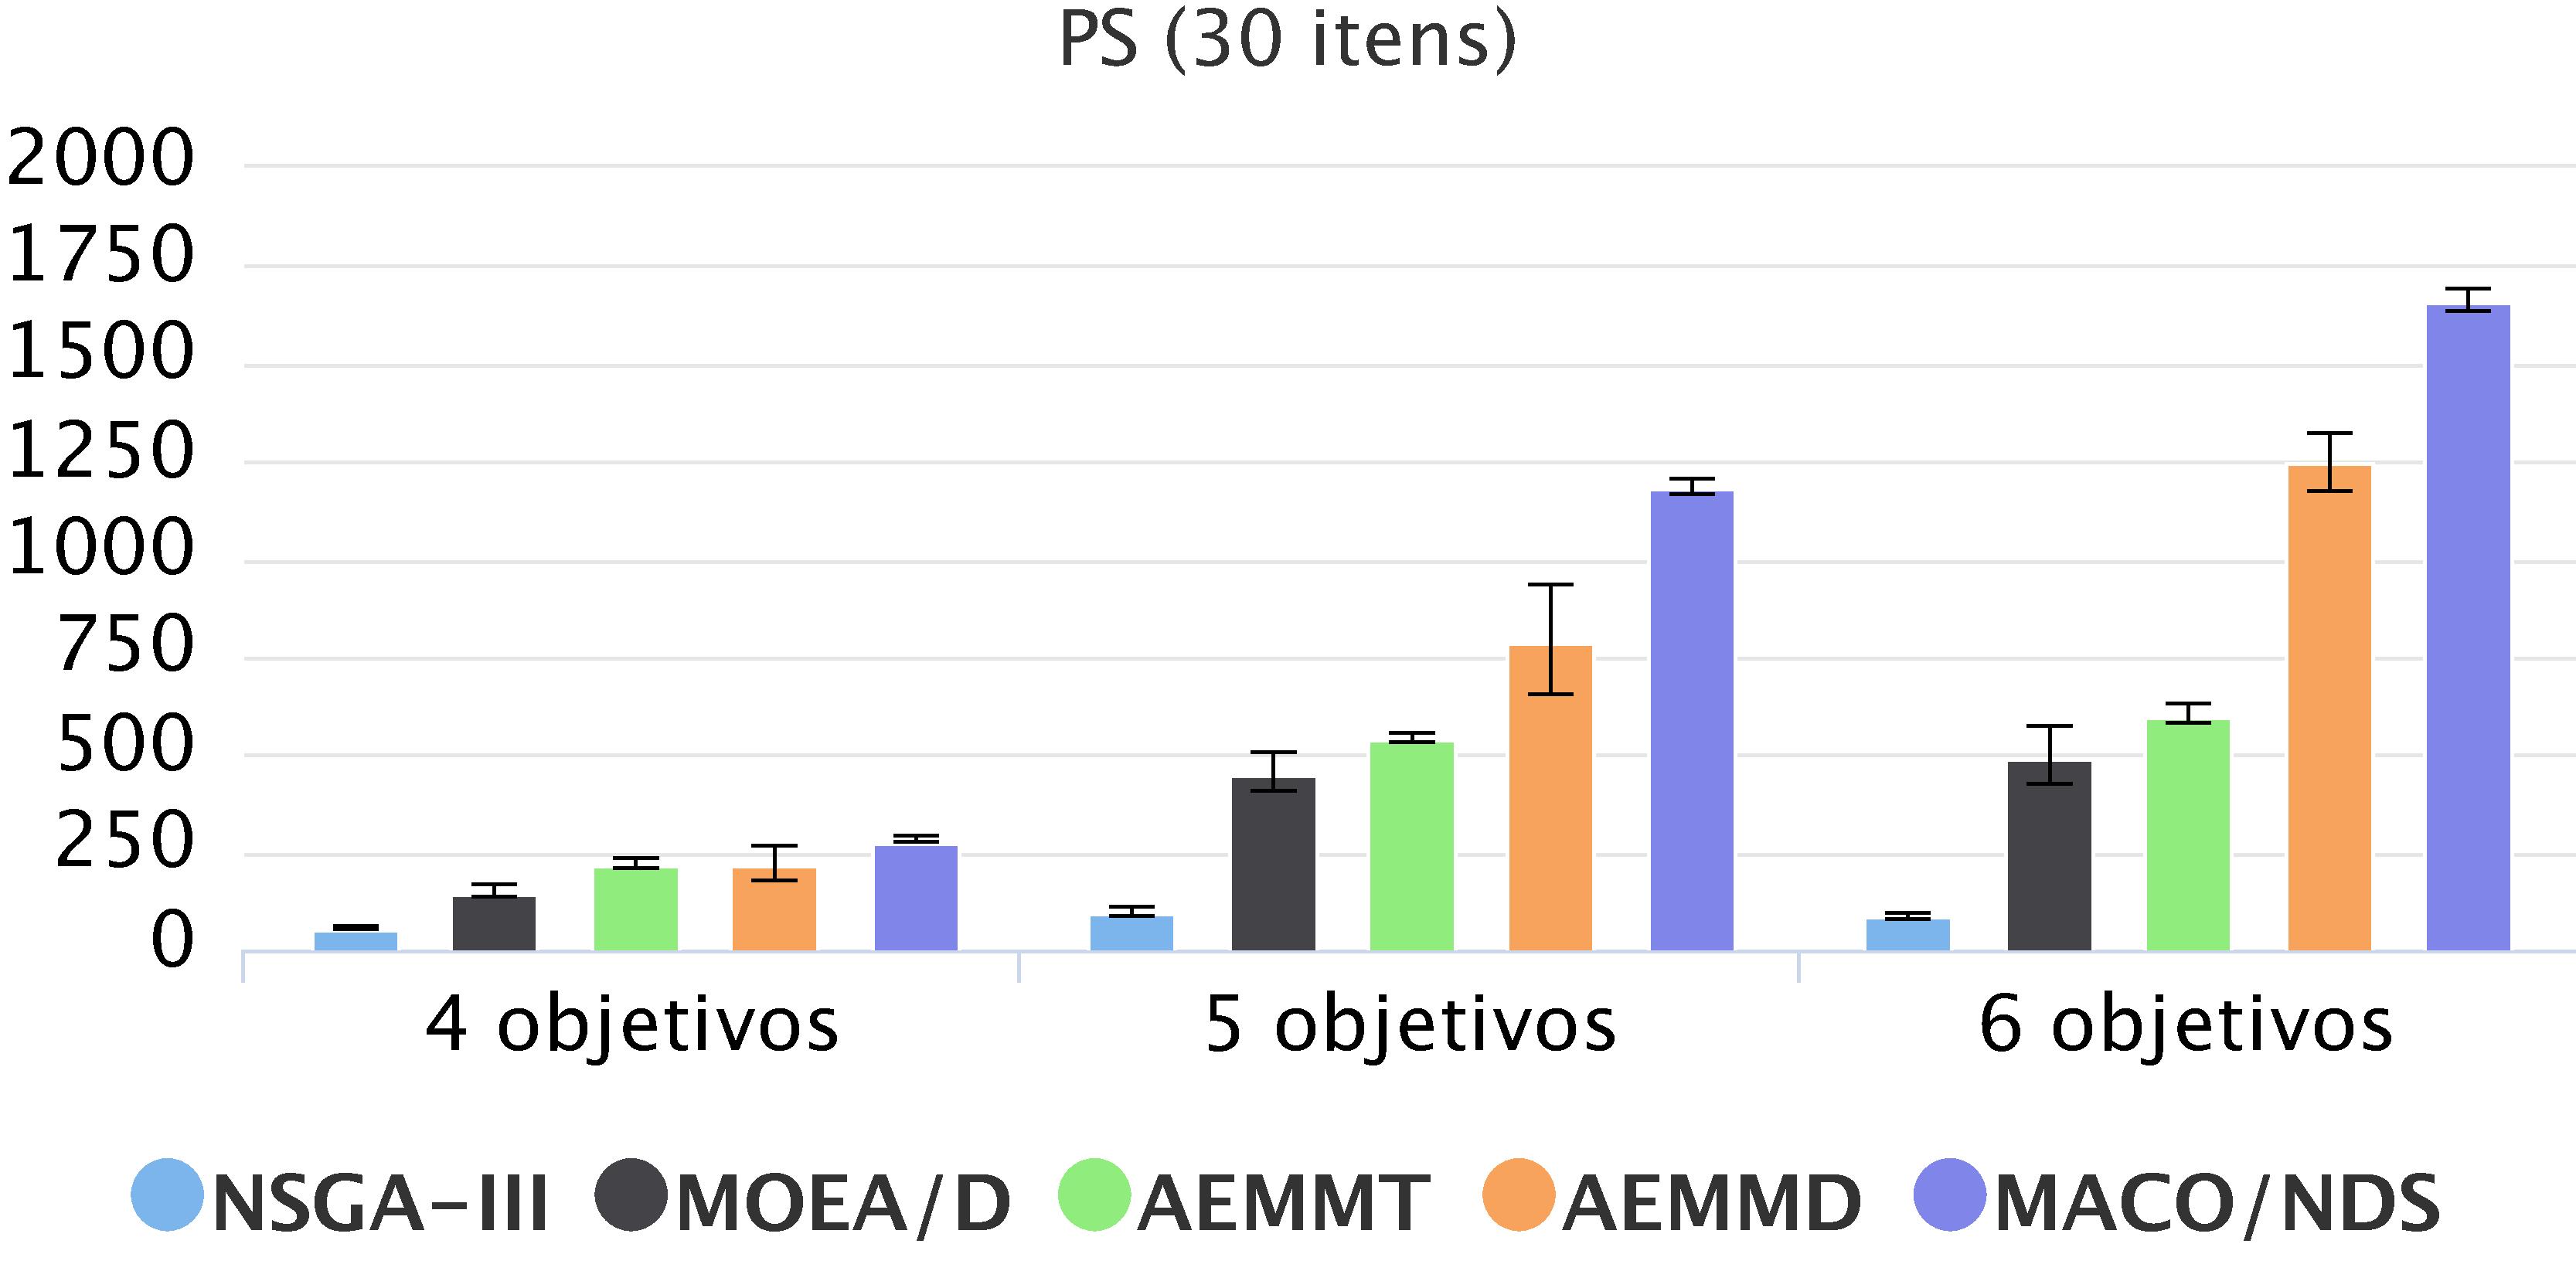
\includegraphics[width=0.5\textwidth]{cap_experimentos/figs/etapa3/ps-mkp-30}
	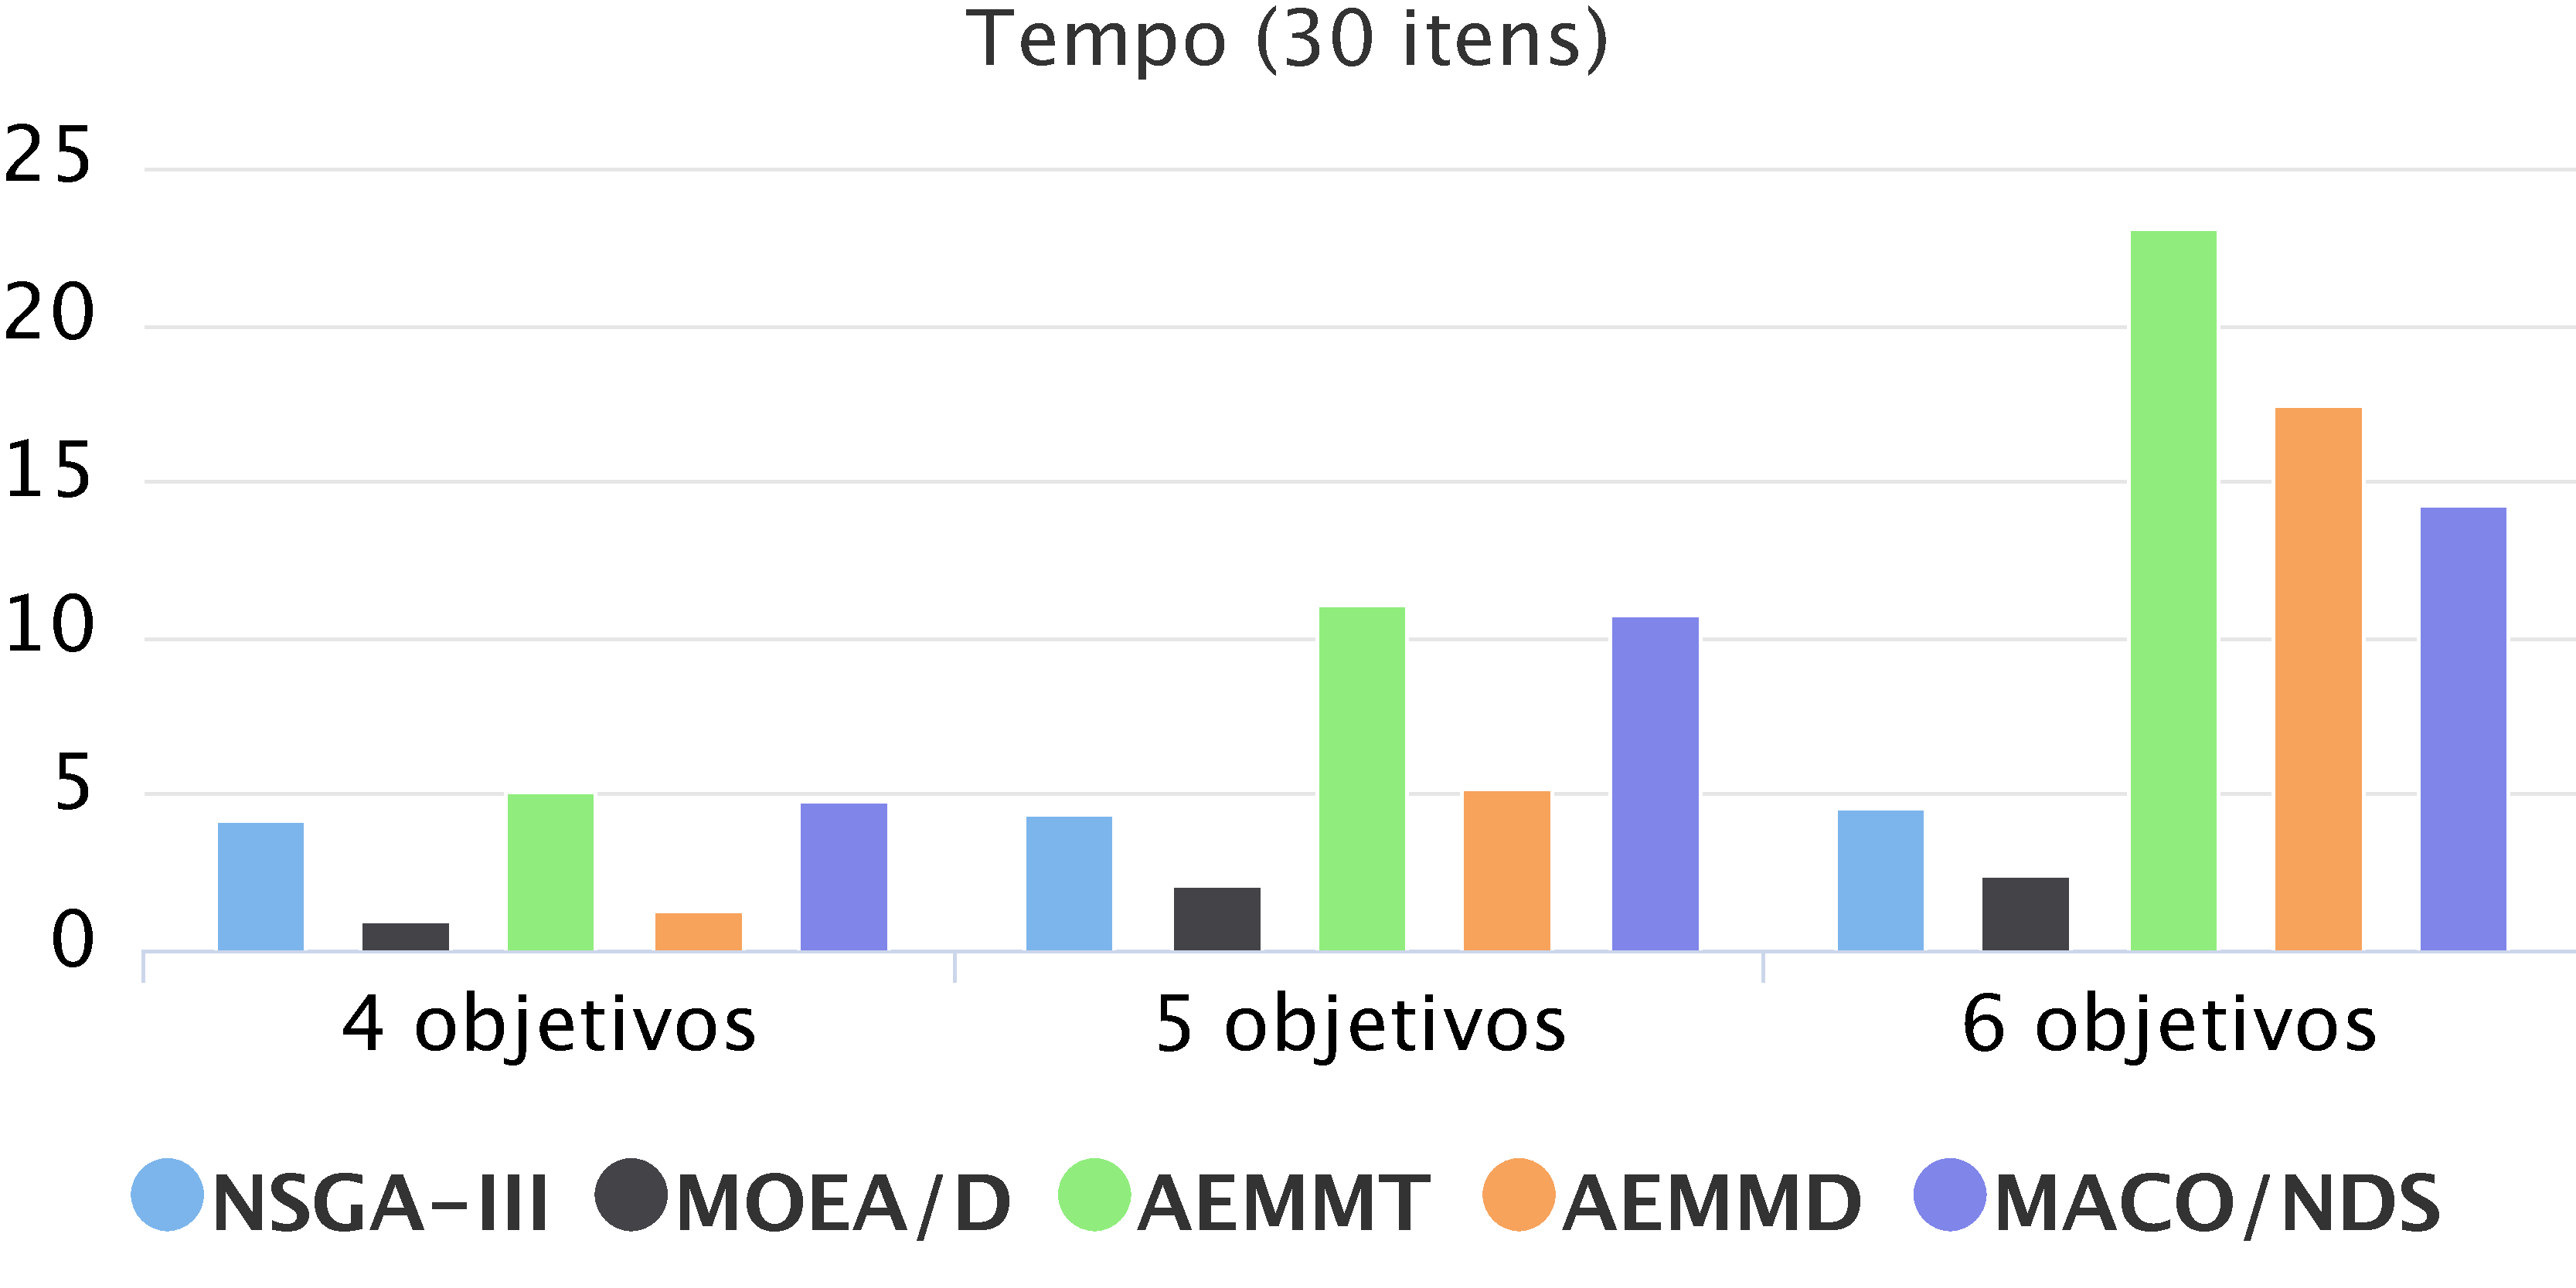
\includegraphics[width=0.5\textwidth]{cap_experimentos/figs/etapa3/time-mkp-30}
	\caption{\label{fig_exp3_pmm_30}Desempenho dos algoritmos na 3ª etapa para o PMM com 30 itens}
\end{figure*}

A \autoref{fig_exp3_pmm_30} retrata a versão mais simples do problema da mochila (30 itens). Nesse cenário, o AEMMT apresenta a menor taxa de erro dentre os algoritmos \textit{many-objective}, seguido pelo MACO/NDS e pelo AEMMD. Considerando a métrica GD e a formulação com 4 objetivos, os melhores resultados são encontrados pelo MOEA/D, seguido pelo MACO/NDS. Com 5 e 6 objetivos, o AEMMD produz o menor $GD$, sendo acompanhado de perto pelo MACO/NDS. Na métrica $PS$, o MACO/NDS é o algoritmo com melhor desempenho para todas as formulações de objetivo. Na sequência, os algoritmos com os melhores valores de $PS$ são: AEMMD, AEMMT, MOEA/D e NSGA-III. Destre esses algoritmos, o único com um limite fixo no tamanho do Pareto é o NSGA-III. Portanto, é esperado que possua um valor de $PS$ menor. Quanto ao tempo, o MOEA/D é o algoritmo mais rápido, enquanto que o AEMMT é o mais lento. O MACO/NDS também demanda um tempo considerável. Seu desempenho nesta métrica é similar ao AEMMT no problema com 4 e 5 objetivos e o terceiro pior com relação ao tempo (atrás do AEMMT e do AEMMD) na formulação com 6 objetivos.

\begin{figure*}[!htbp]	
	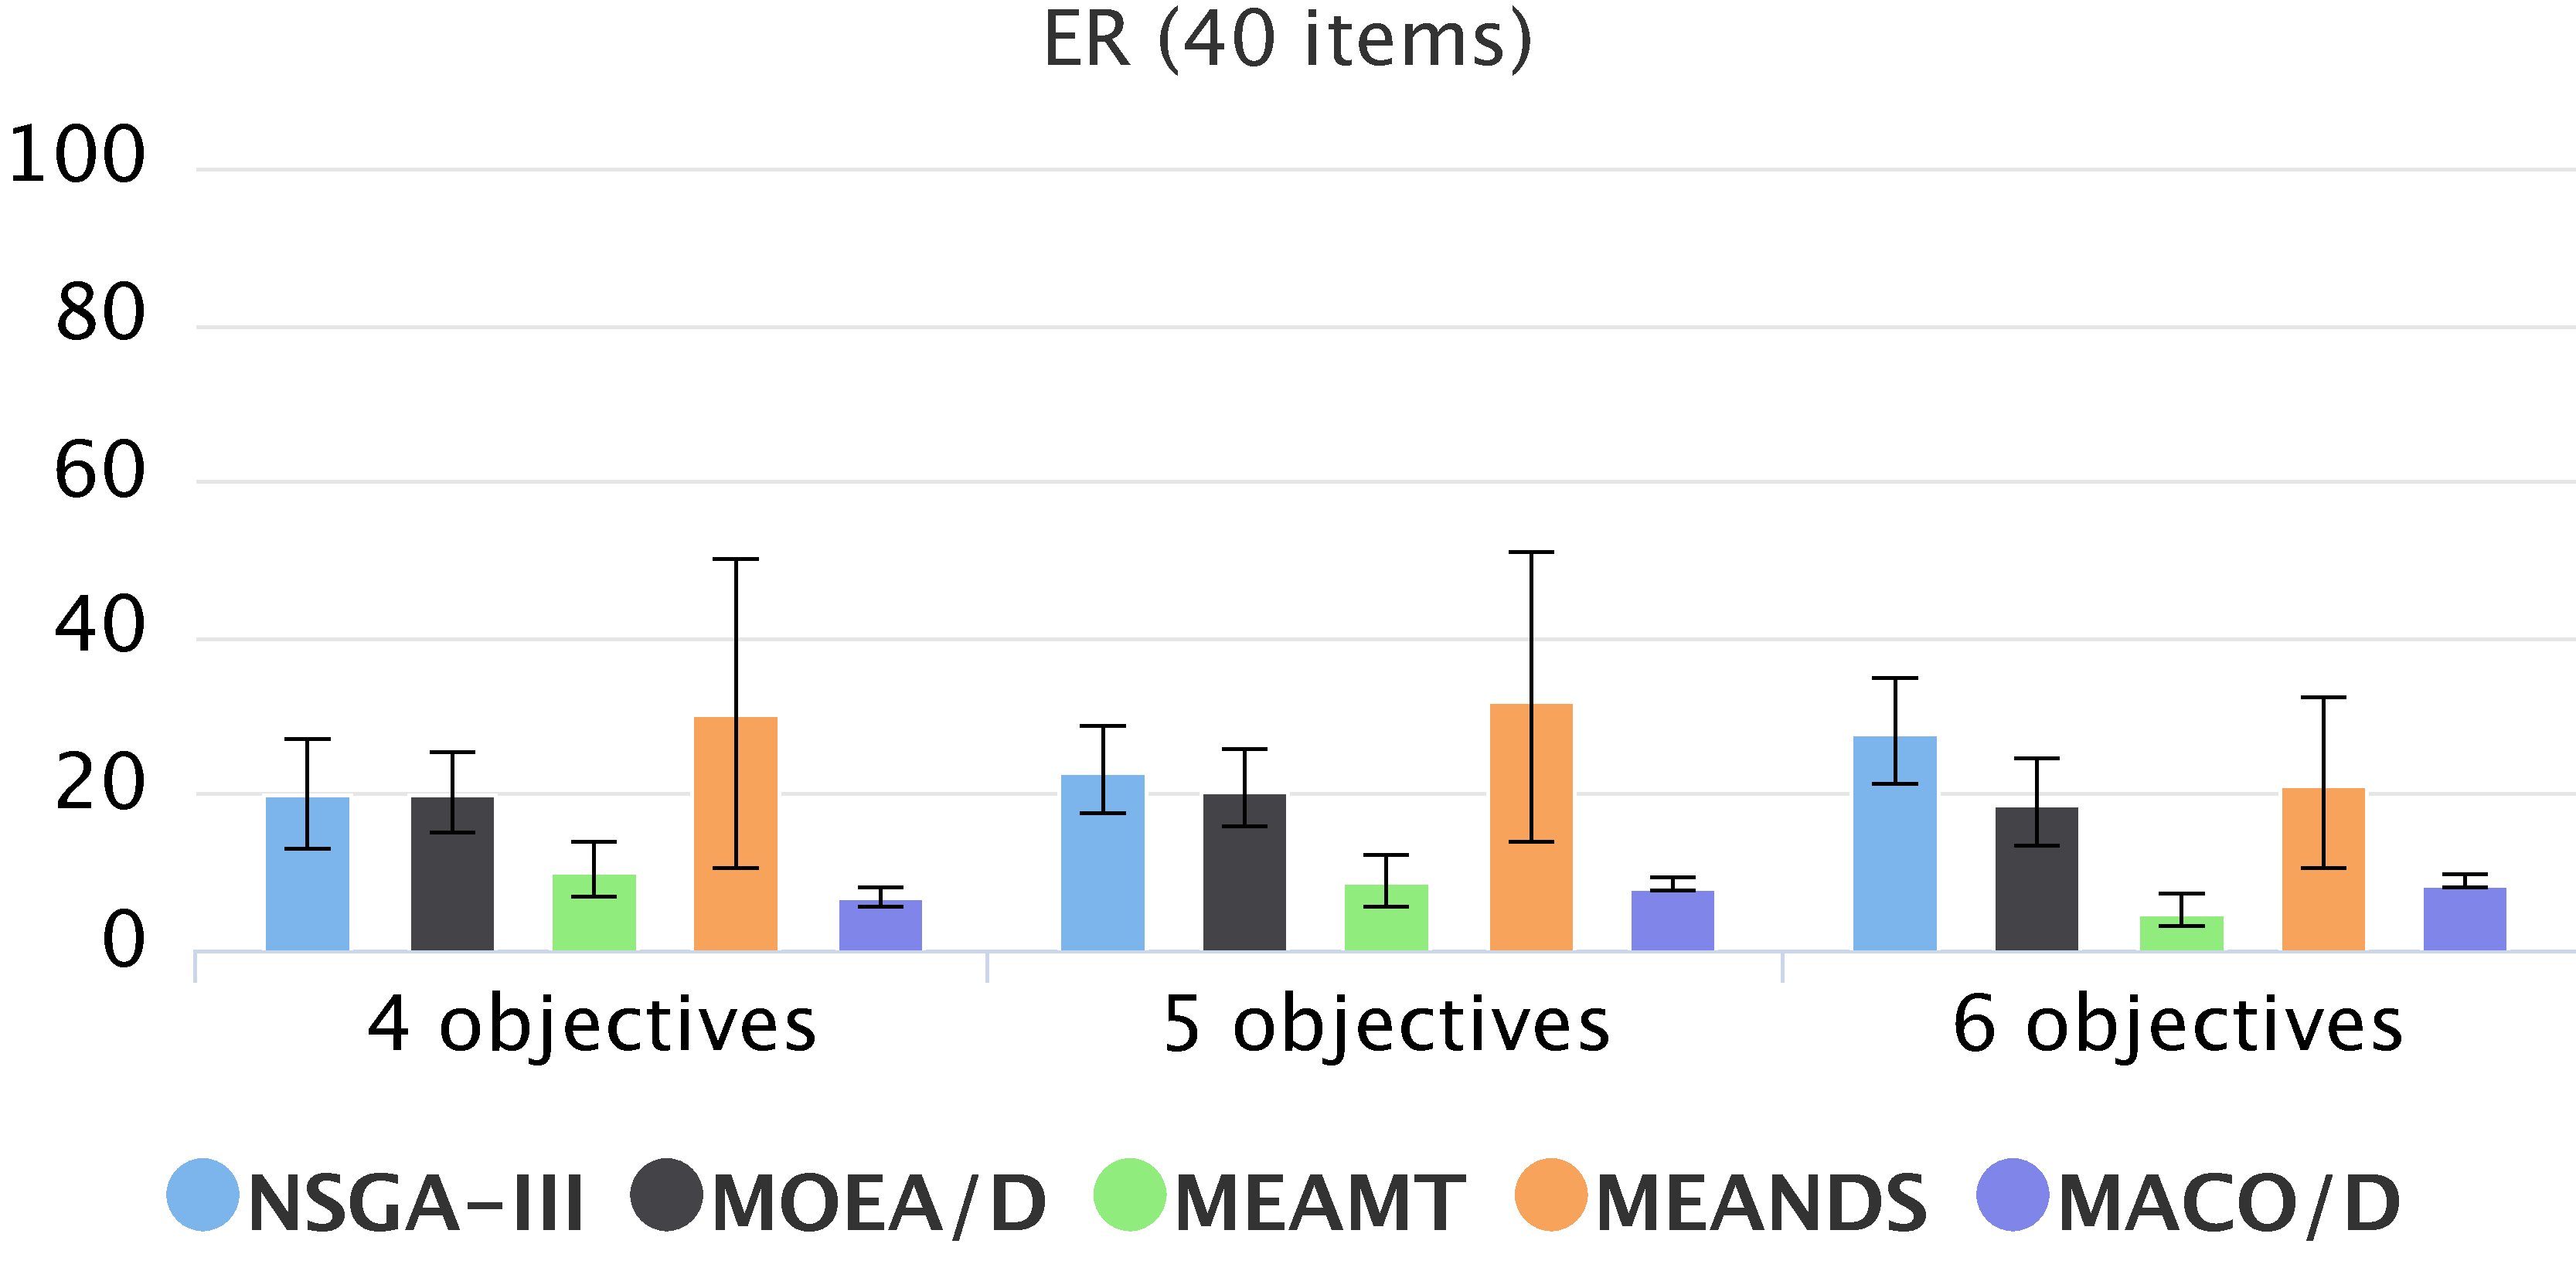
\includegraphics[width=0.5\textwidth]{cap_experimentos/figs/etapa3/er-mkp-40}
	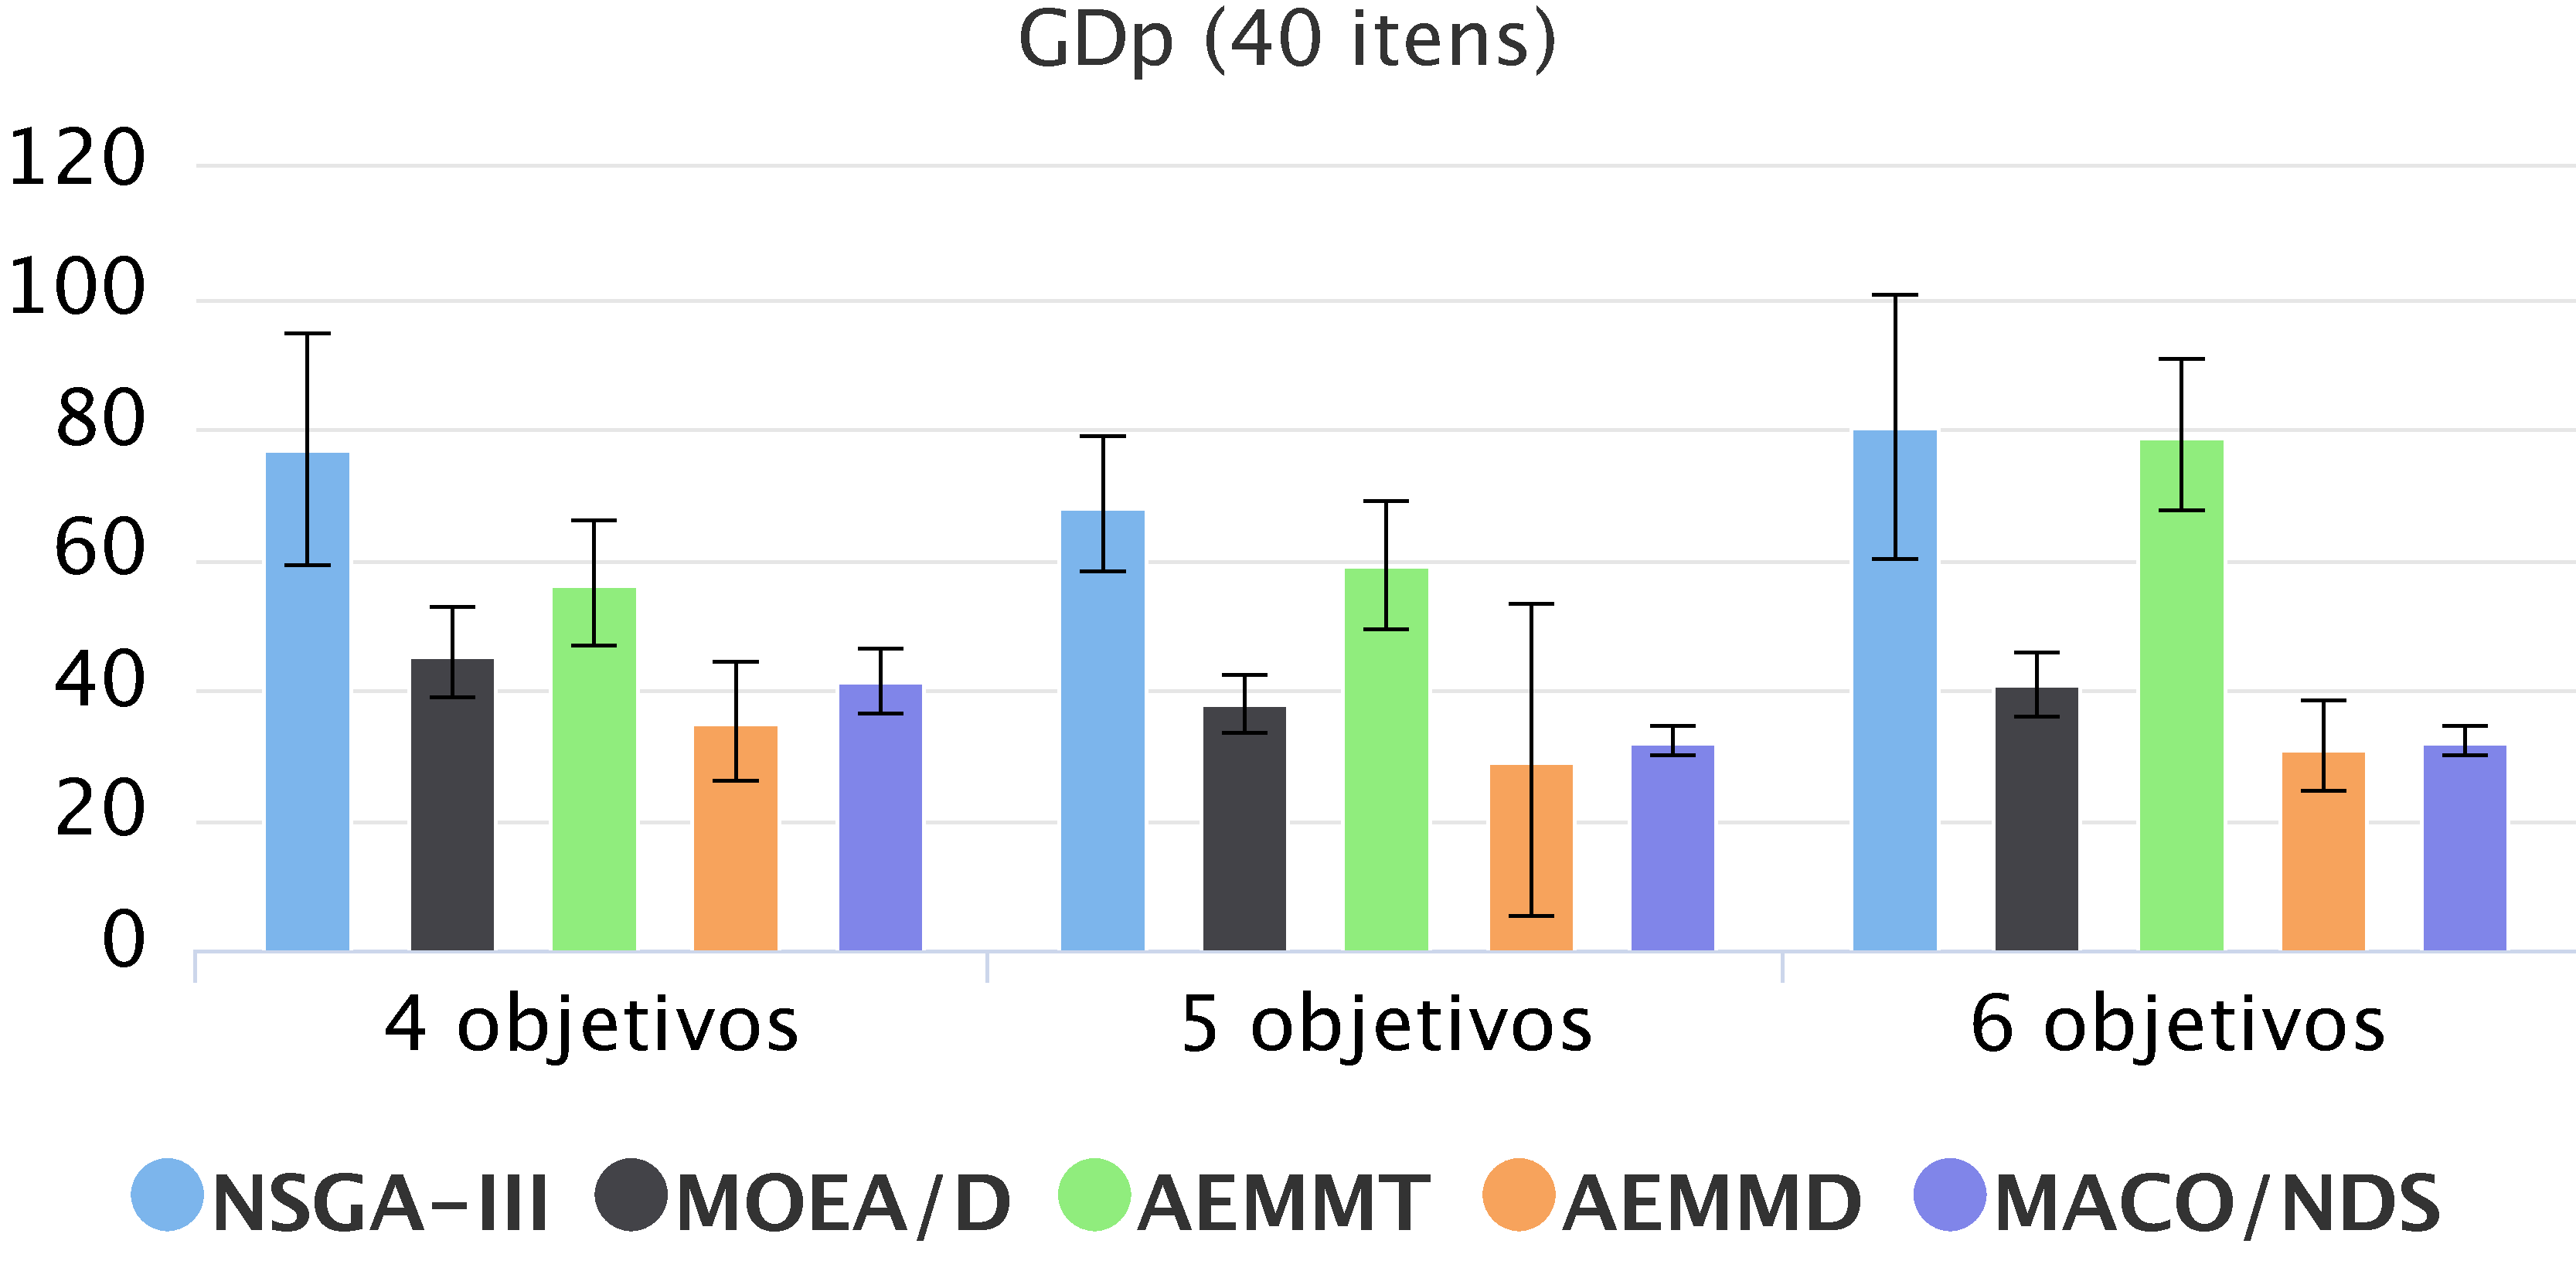
\includegraphics[width=0.5\textwidth]{cap_experimentos/figs/etapa3/gd-mkp-40}
	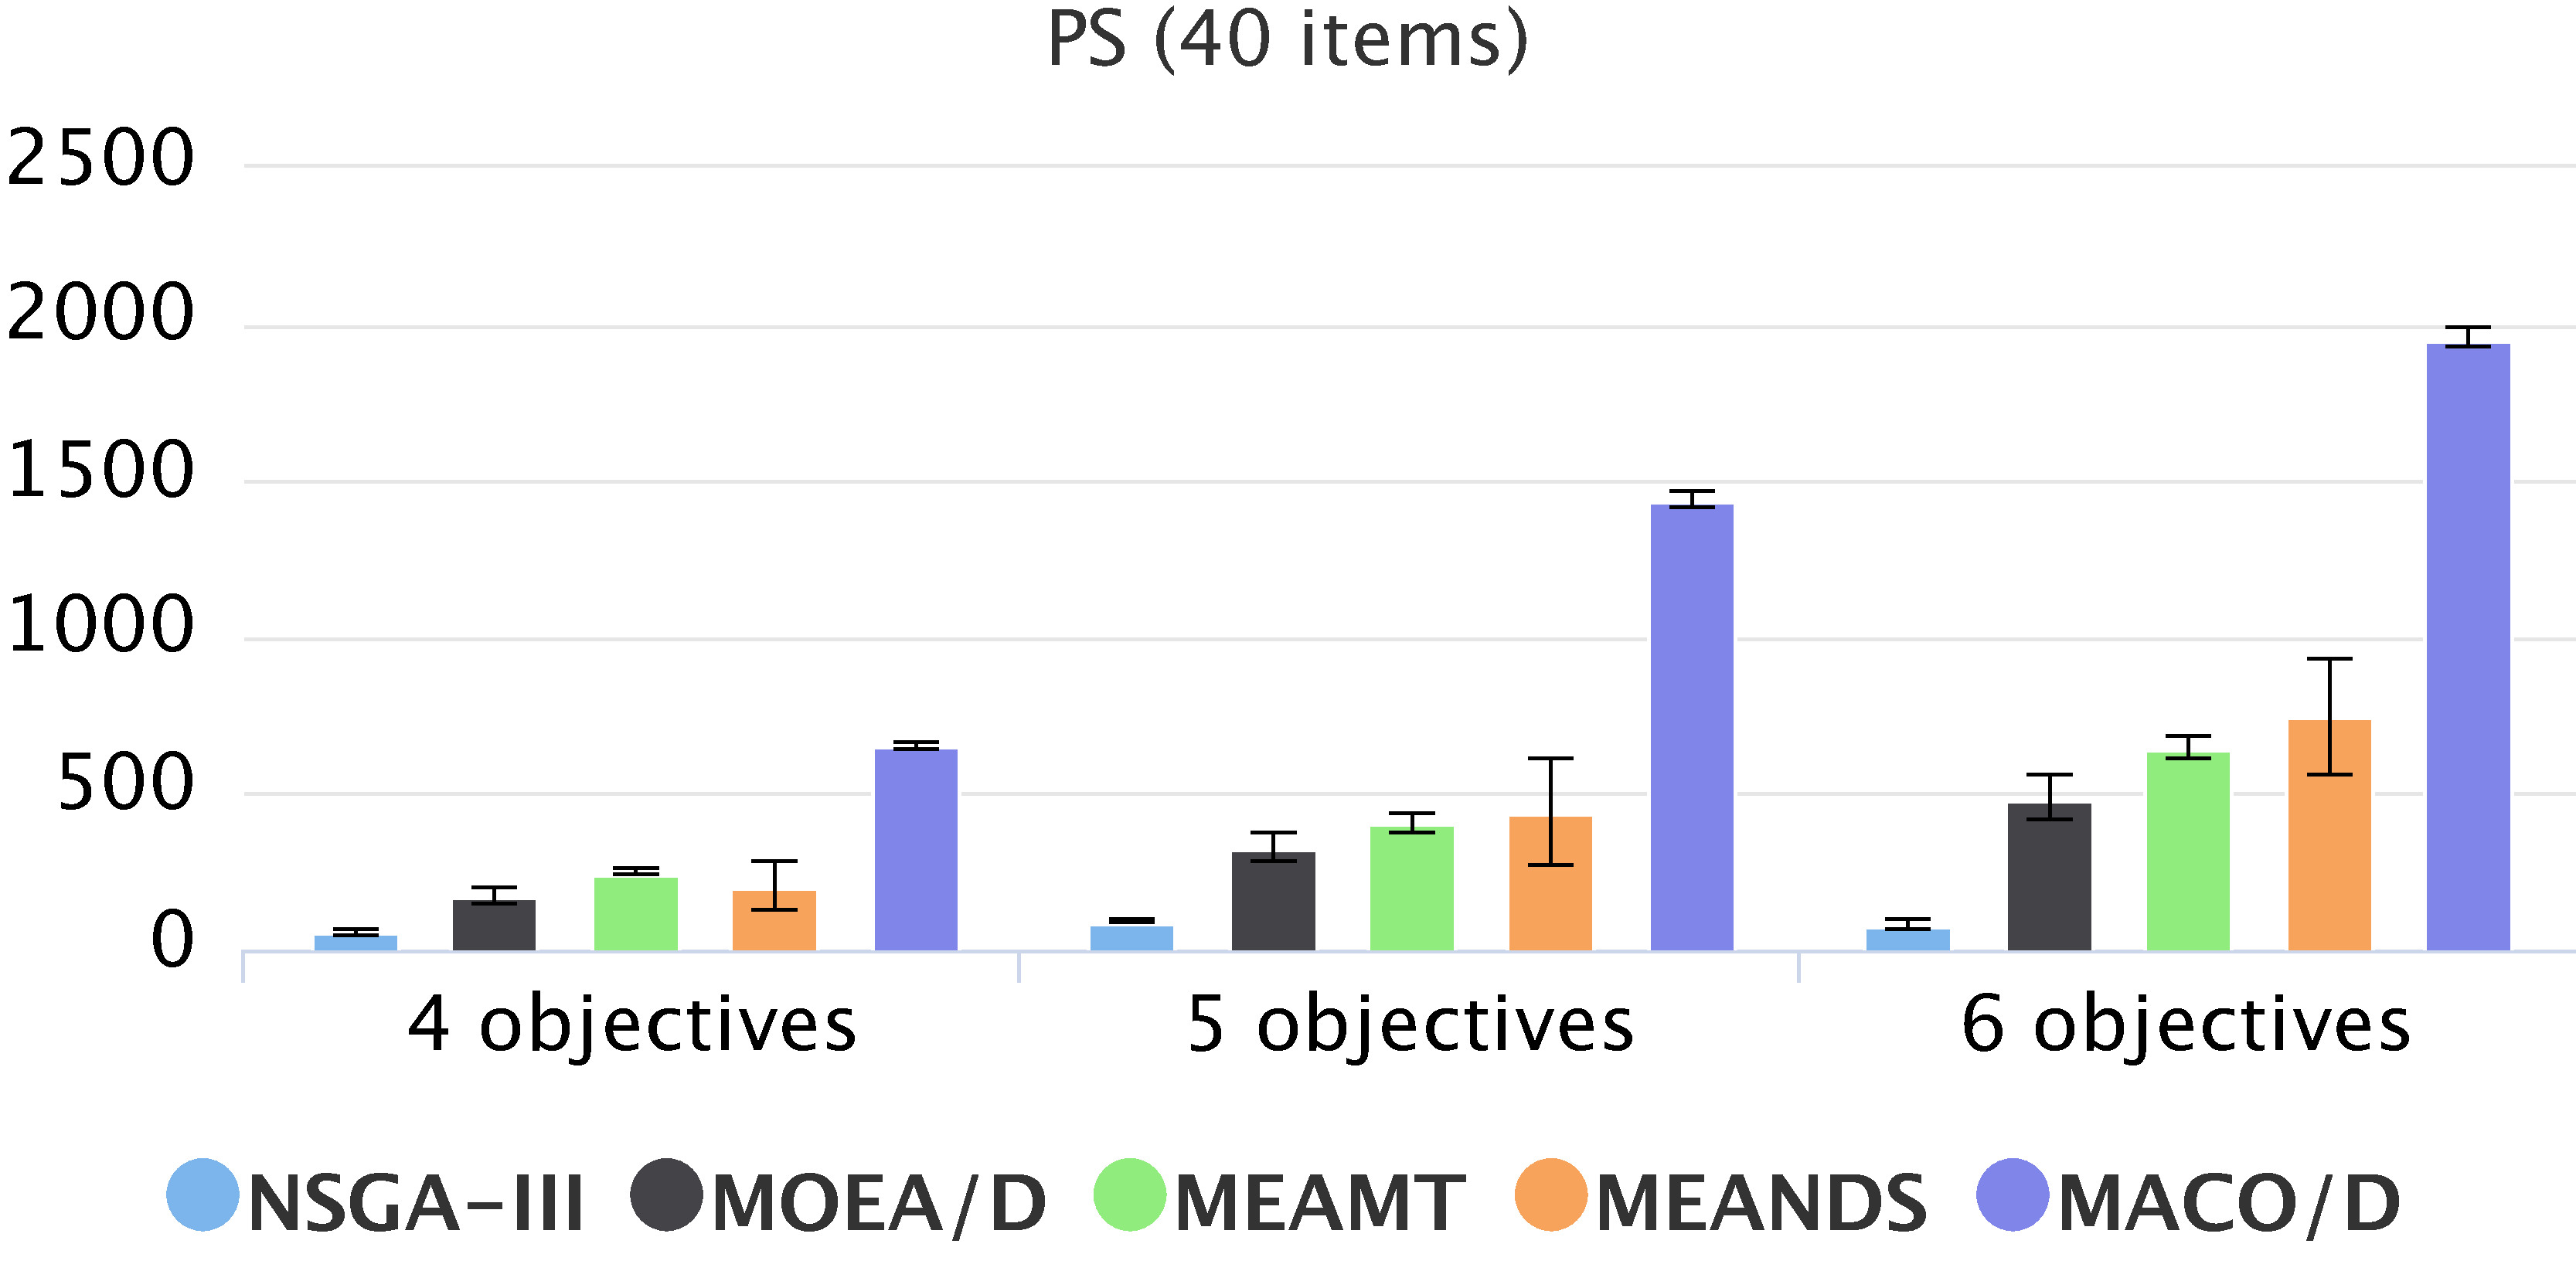
\includegraphics[width=0.5\textwidth]{cap_experimentos/figs/etapa3/ps-mkp-40}
	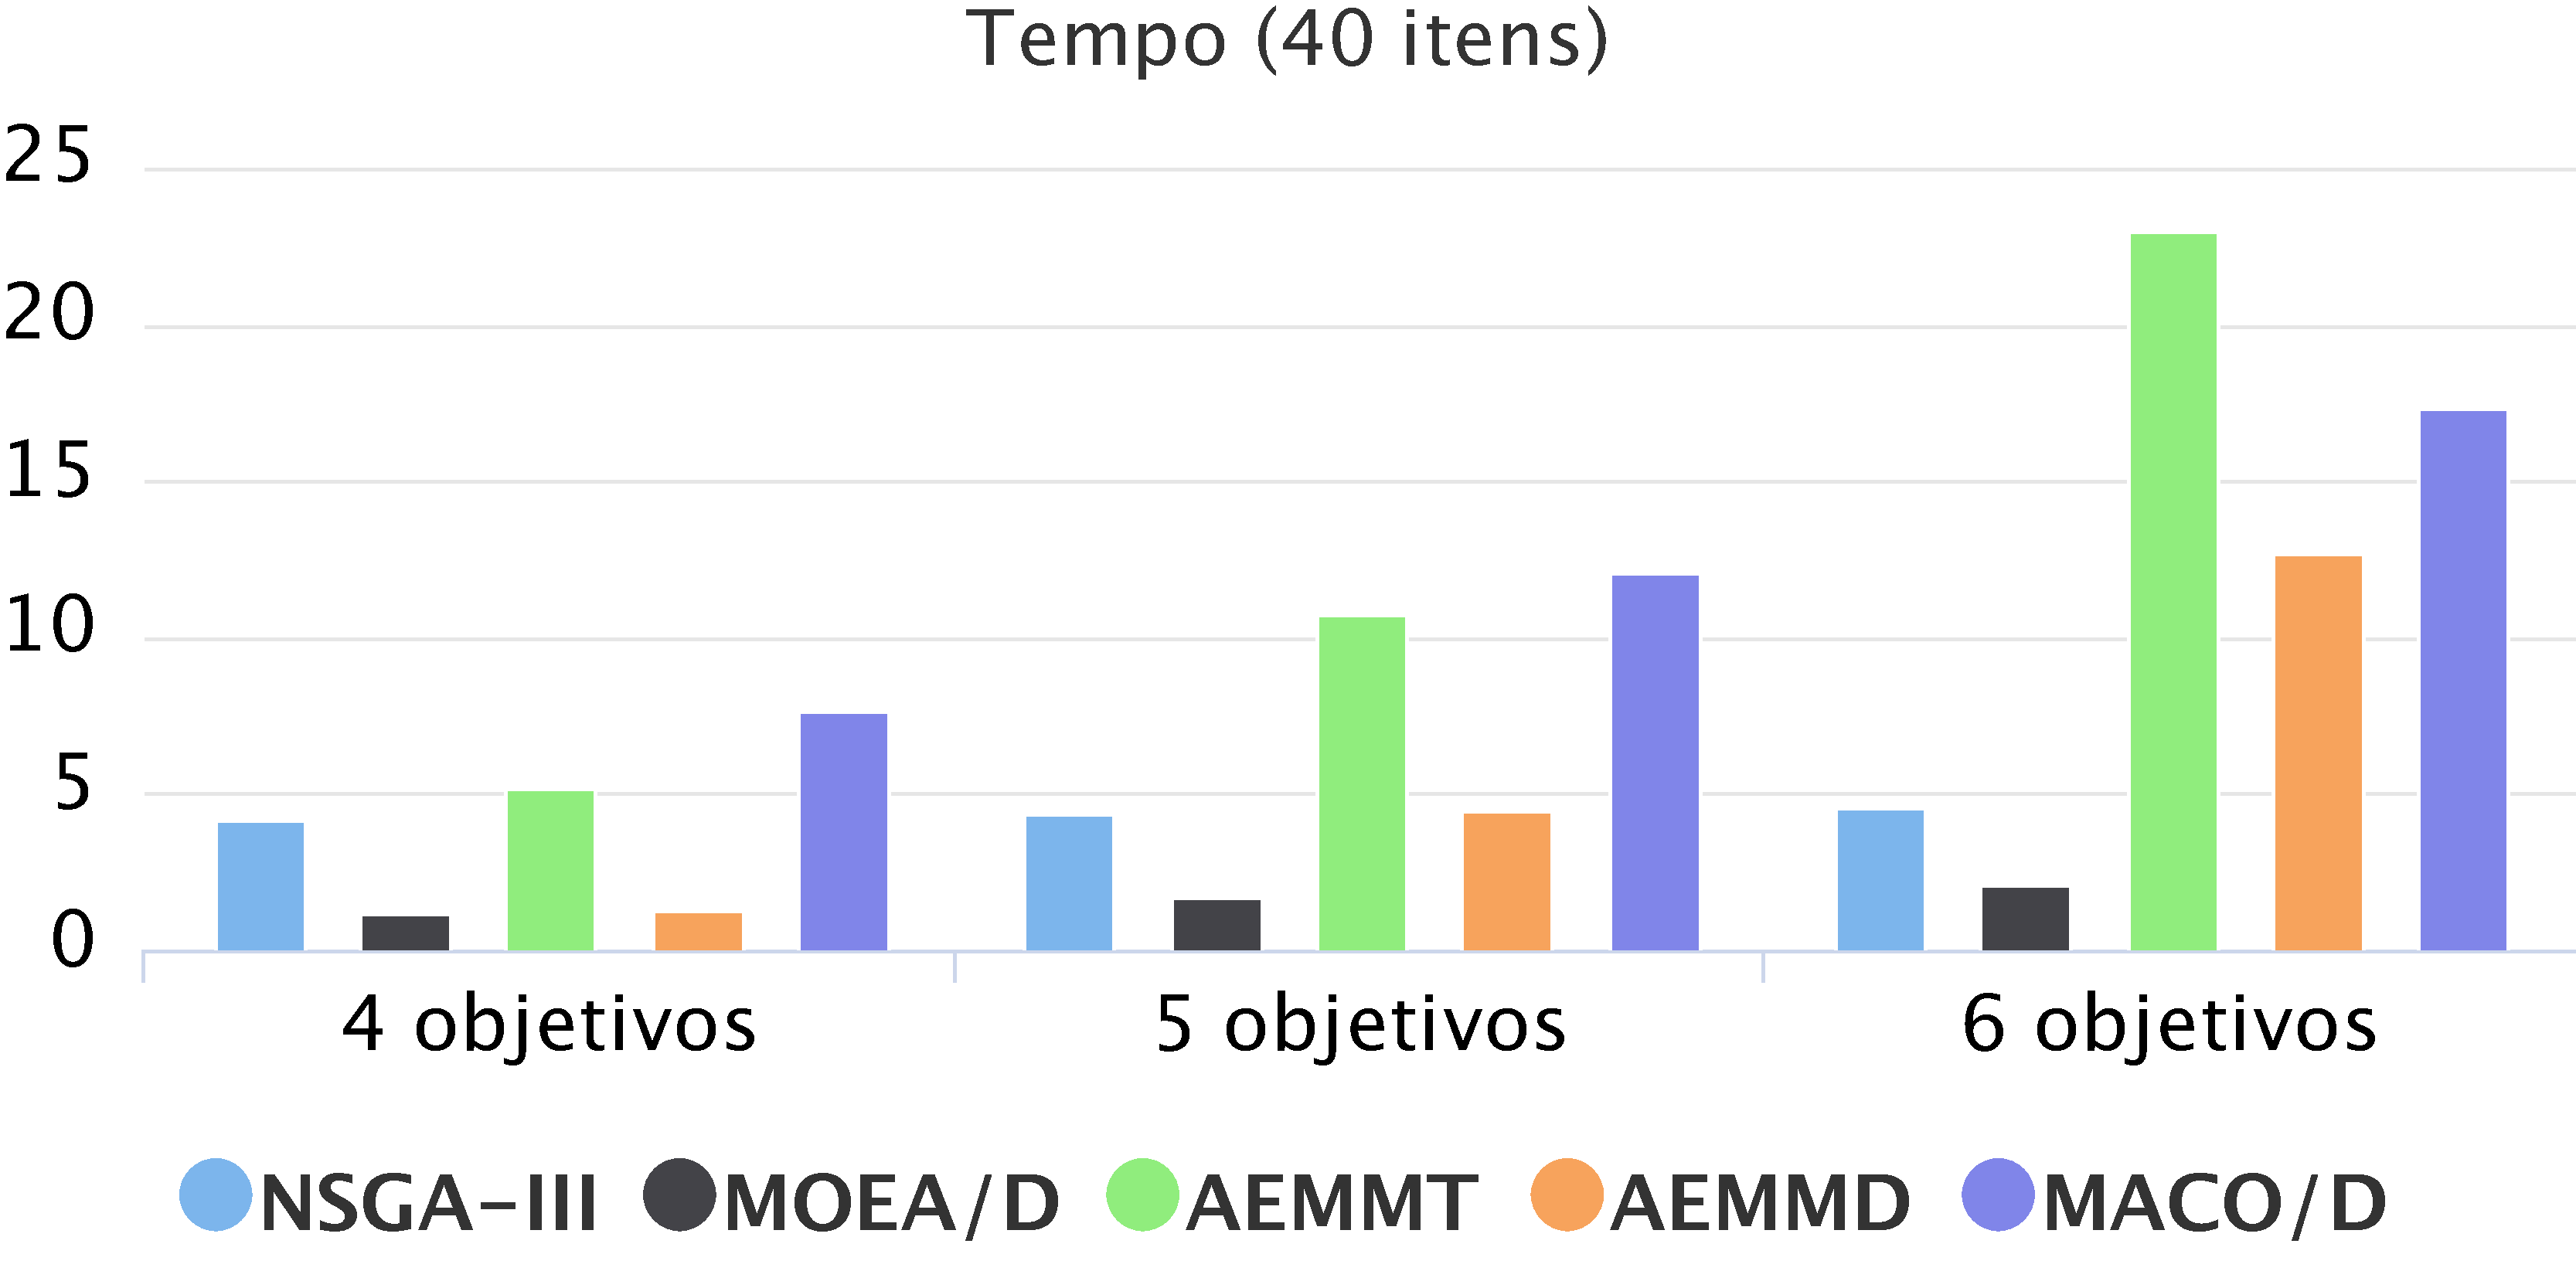
\includegraphics[width=0.5\textwidth]{cap_experimentos/figs/etapa3/time-mkp-40}
	\caption{\label{fig_exp3_pmm_40}Desempenho dos algoritmos na 3ª etapa para o PMM com 40 itens}
\end{figure*}

Os resultados obtidos para o PMM de 40 itens é apresentado na \autoref{fig_exp3_pmm_40}. O AEMMT e o MACO/NDS apresentam as menores taxas de erro, sendo que o MACO/NDS é melhor para 4 e 5 objetivos (6,9\% e 8,4\%, respectivamente), enquanto o AEMMT obtém o melhor resultado para 6 objetivos (5,1\% contra 8,7\% do MACO/NDS). Os melhores valores de $GD$ foram encontrados pelo AEMMD e MACO/NDS, sendo o primeiro um pouco melhor que o segundo. Em contrapartida, o AEMMD apresenta uma alta variação nos resultados, indicando que algumas execuções produz soluções muito próximas do Pareto enquanto outras nem tanto. Considerando o tamanho dos Paretos encontrados ($PS$), novamente o MACO/NDS retorna os melhores valores independente da formulação de objetivos. Em termos do tempo médio de execução, o MOEA/D é o algoritmo mais rápido (5,2 segundos ao somar o tempo das 3 formulações de objetivos), enquanto o AEMMT e o MACO/NDS são os mais lentos (39 e 37,2 segundos, ao somar o tempo das 3 formulações de objetivos, respectivamente).

\begin{figure*}[!htbp]
	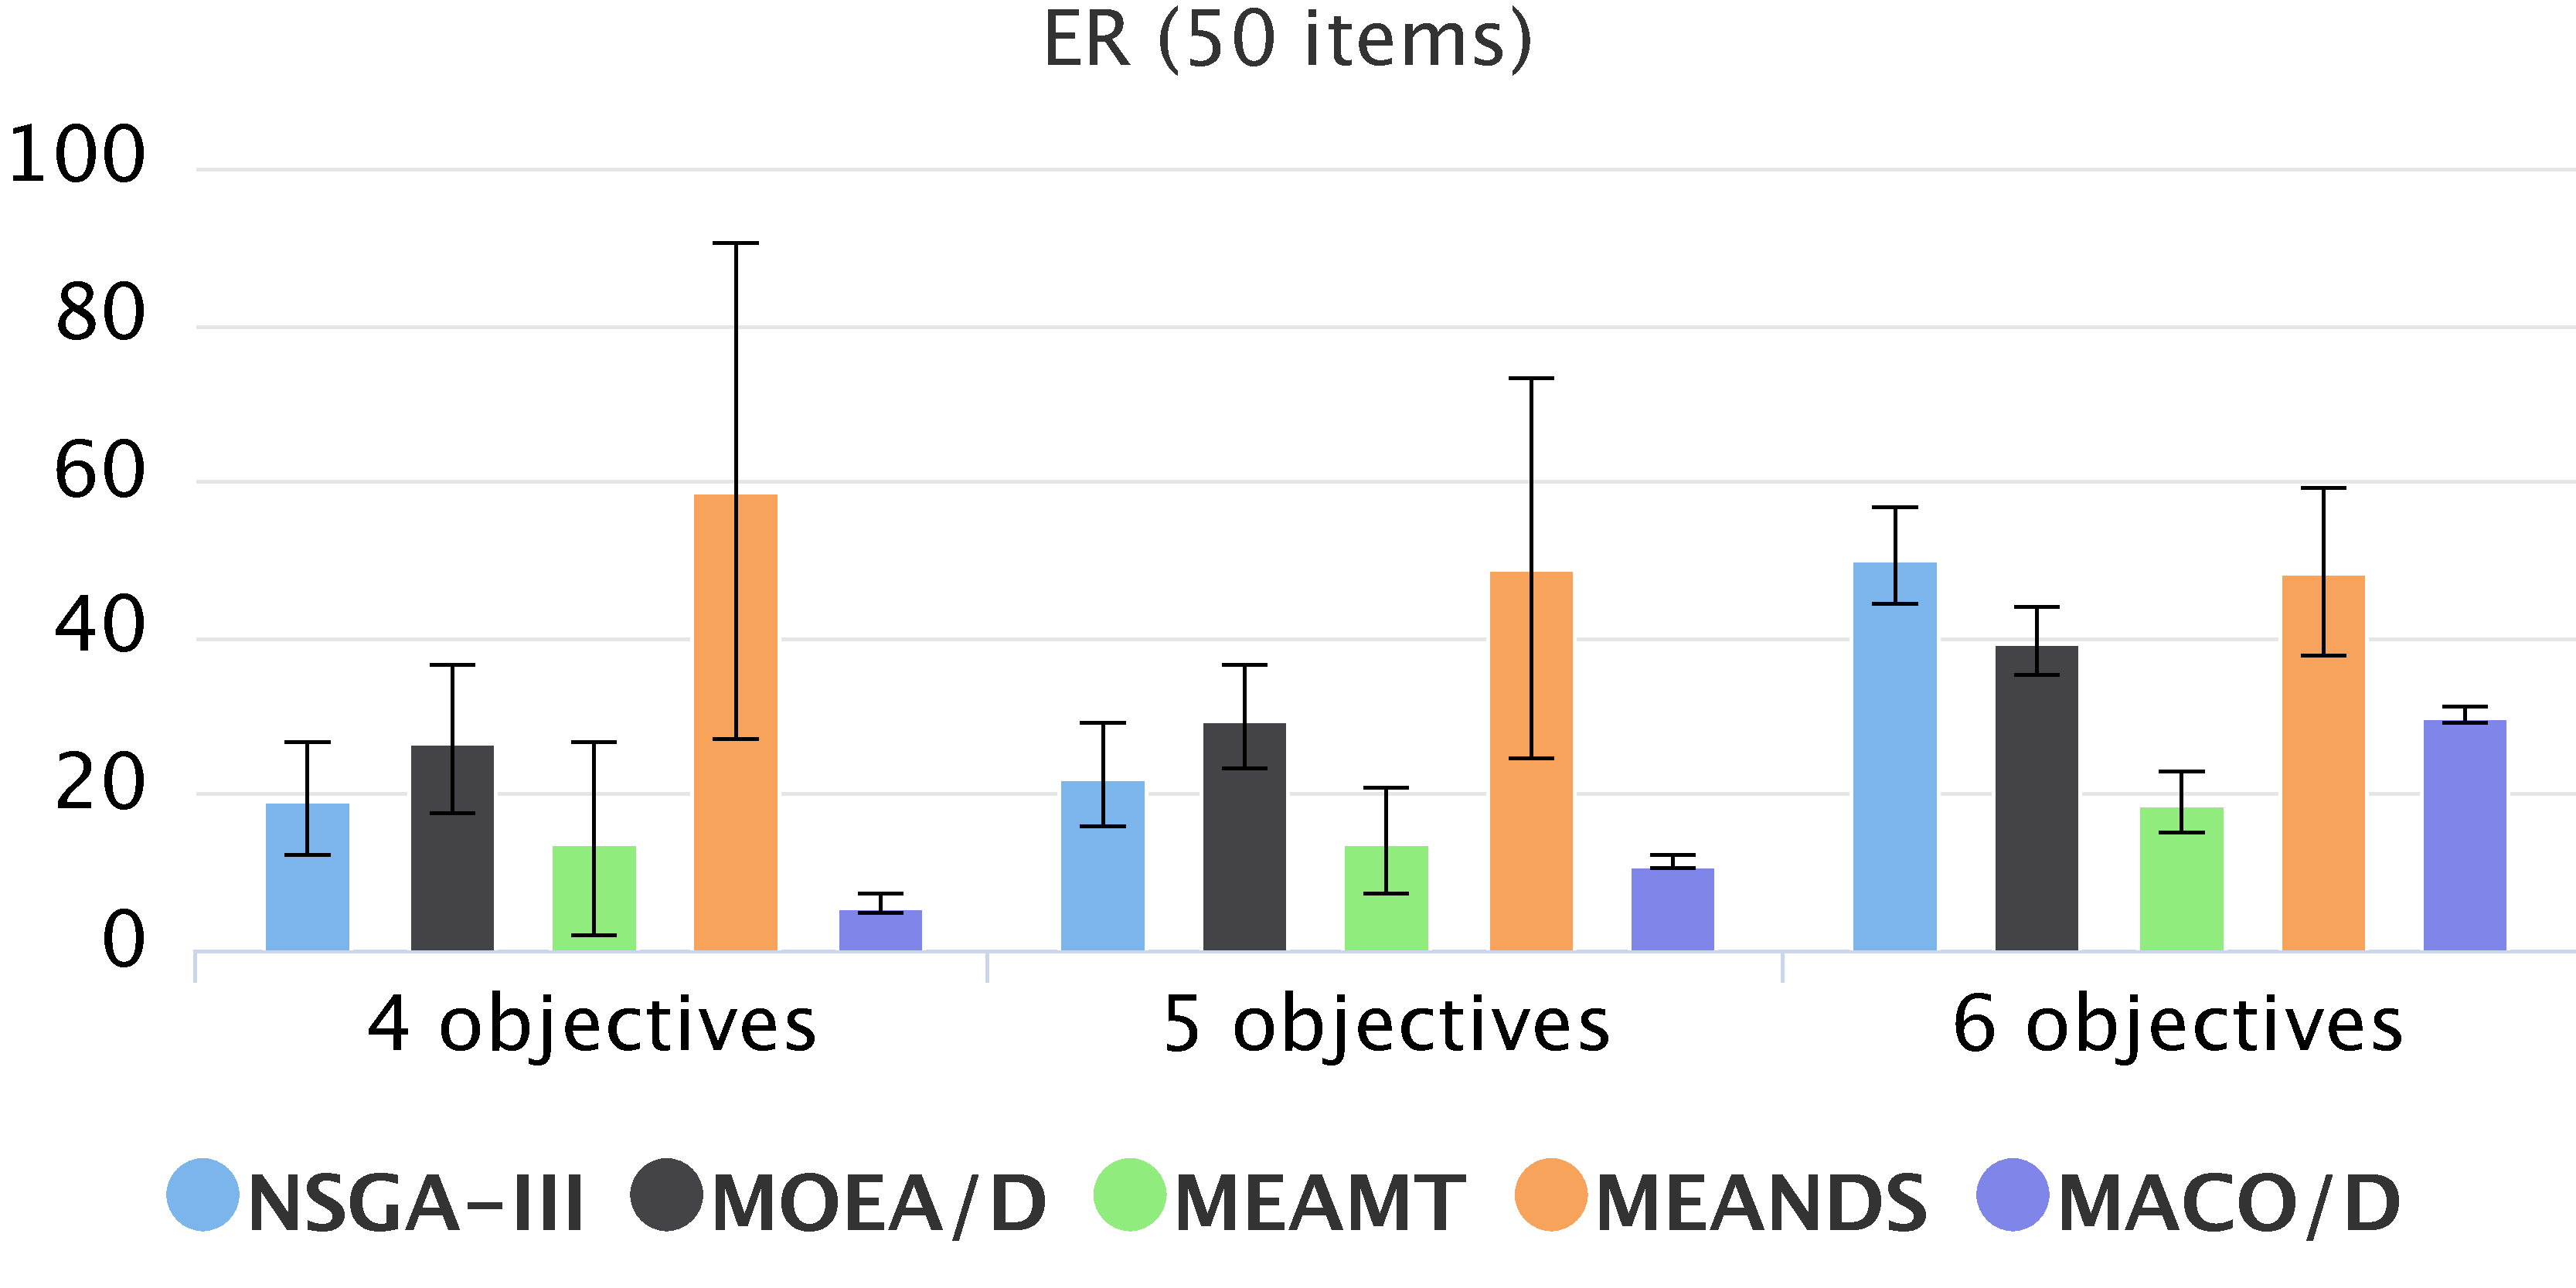
\includegraphics[width=0.5\textwidth]{cap_experimentos/figs/etapa3/er-mkp-50}
	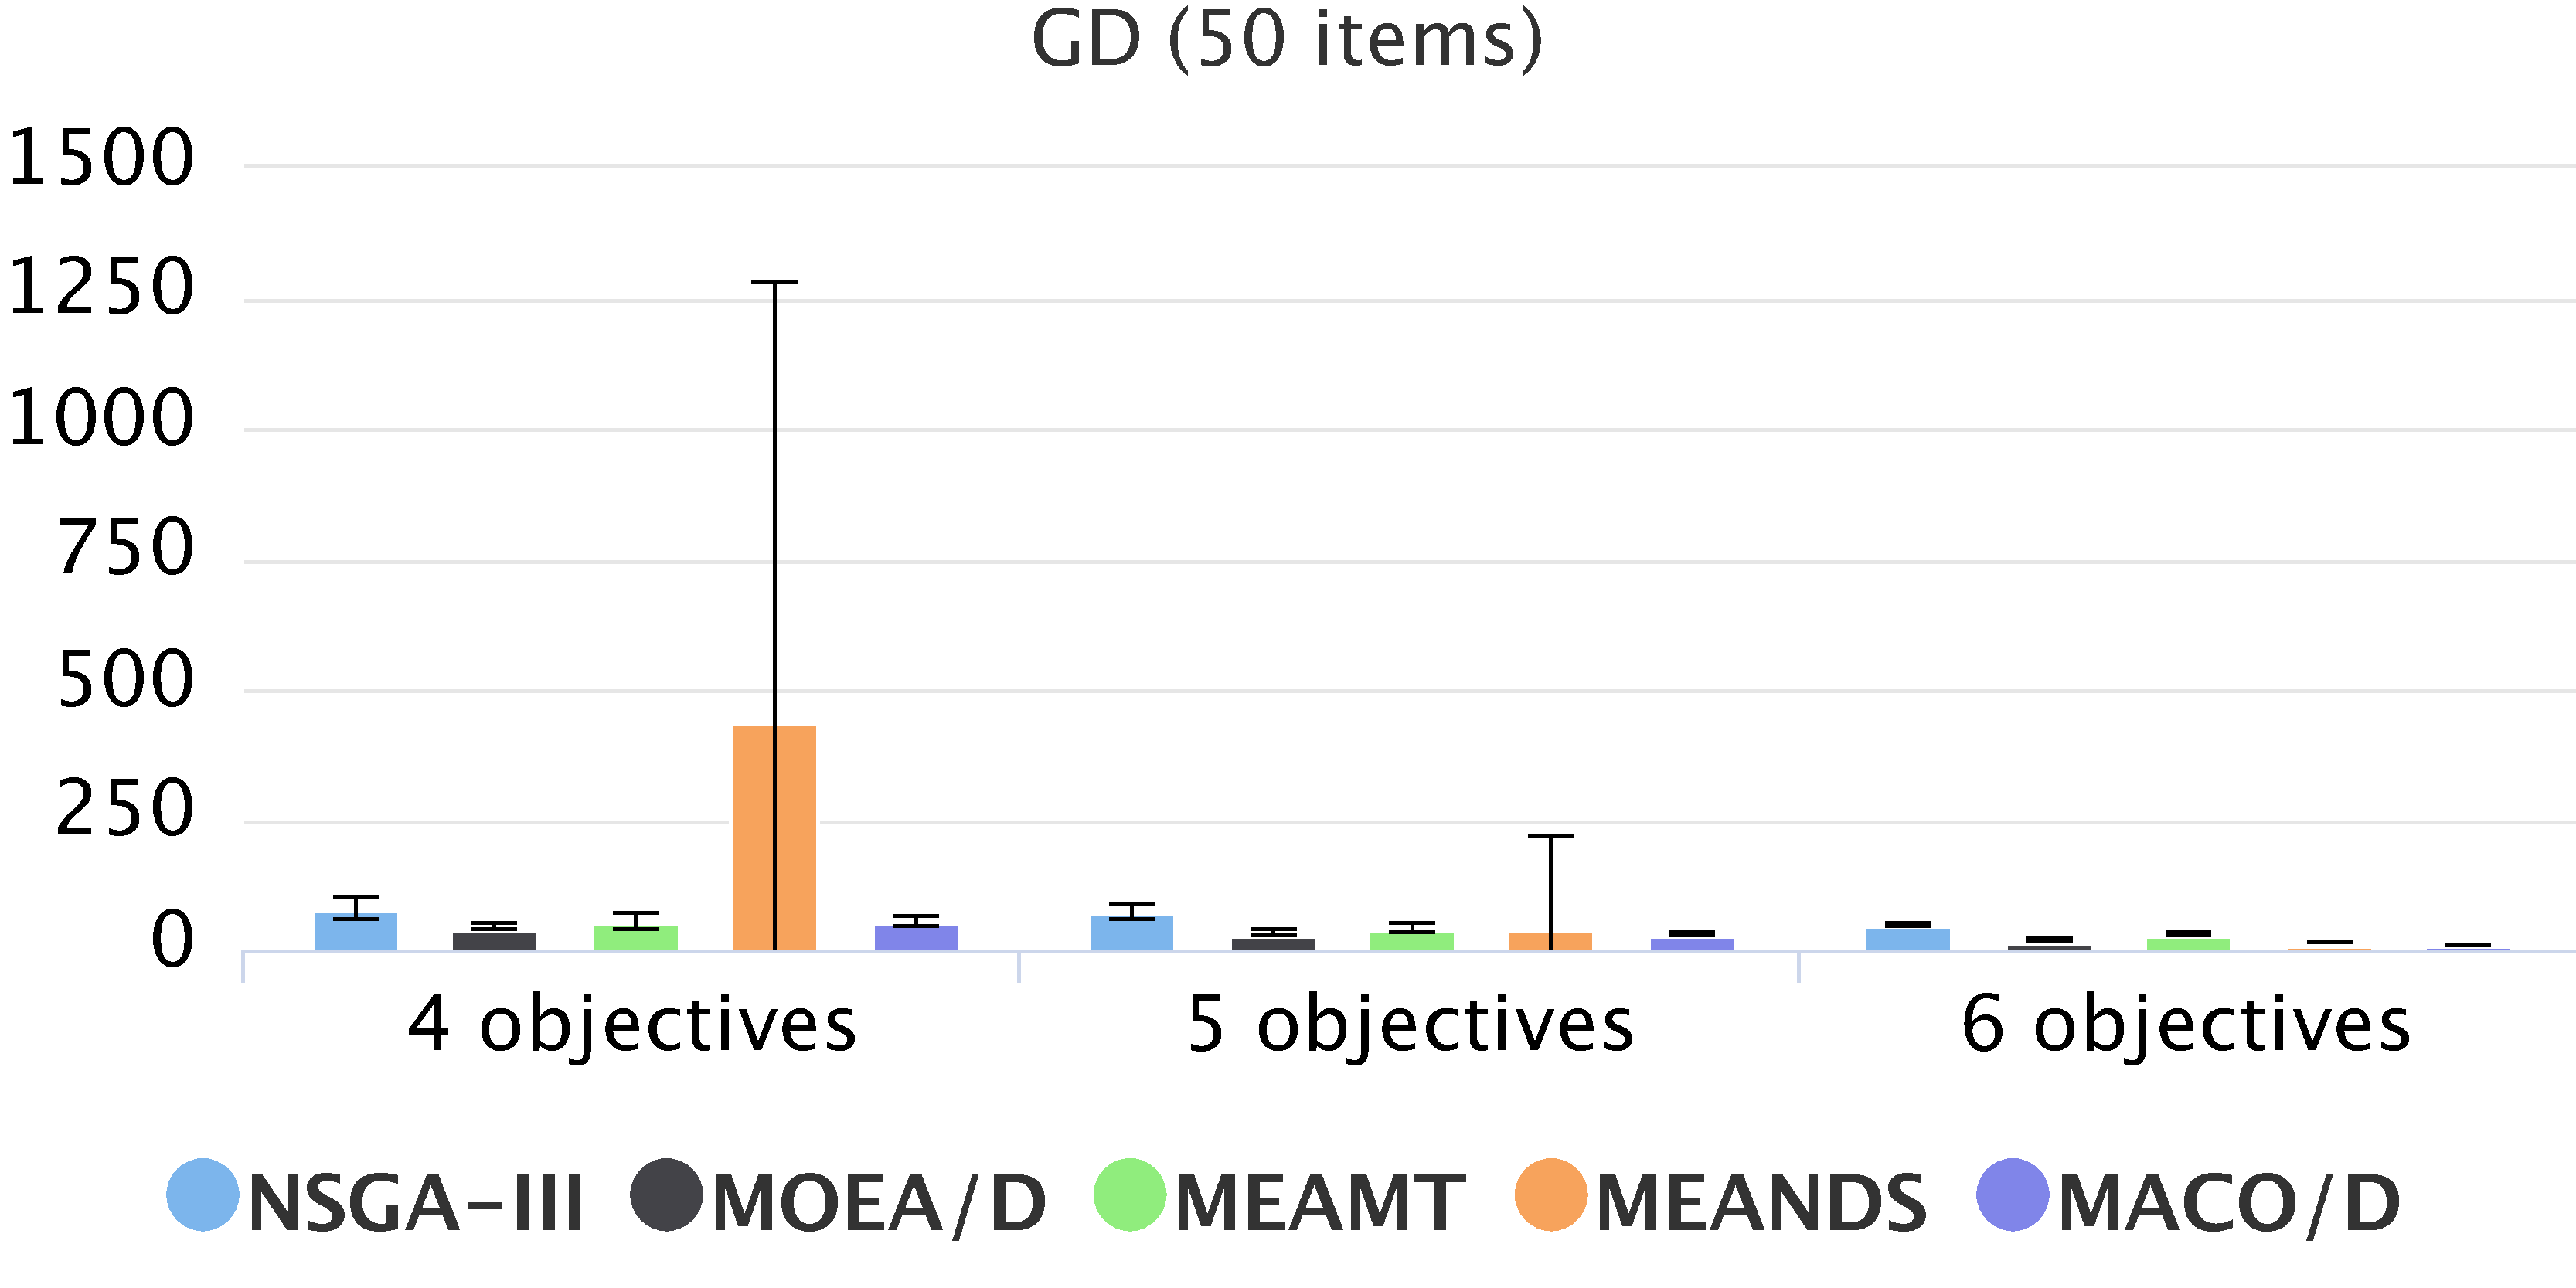
\includegraphics[width=0.5\textwidth]{cap_experimentos/figs/etapa3/gd-mkp-50}
	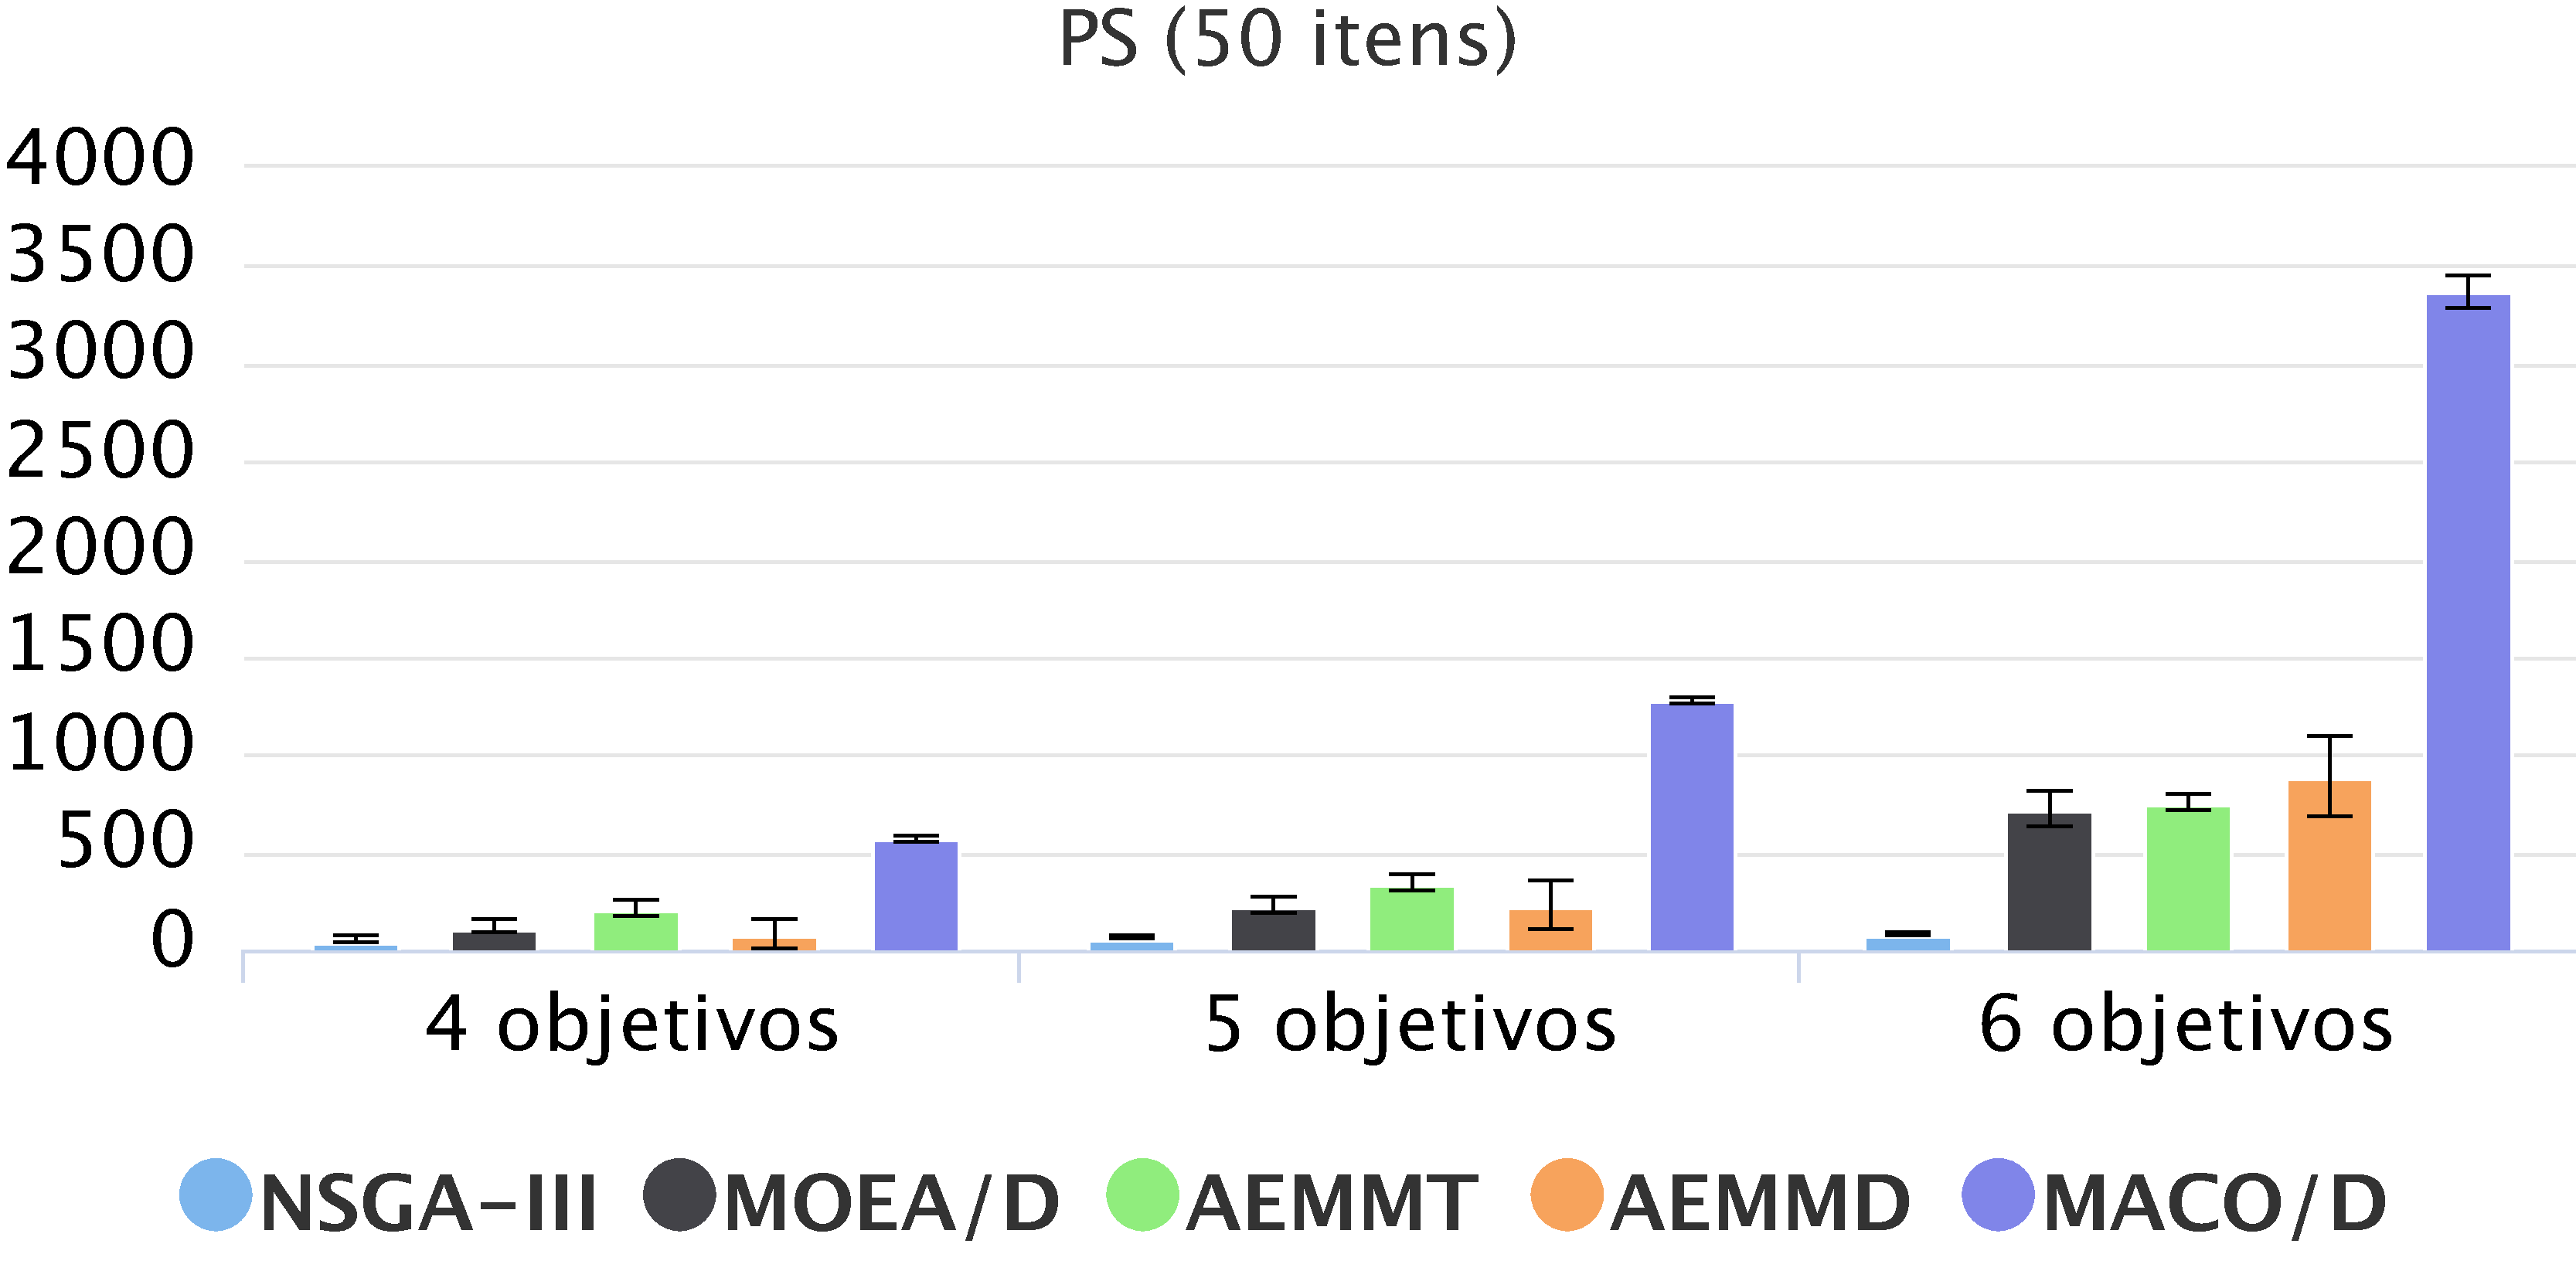
\includegraphics[width=0.5\textwidth]{cap_experimentos/figs/etapa3/ps-mkp-50}
	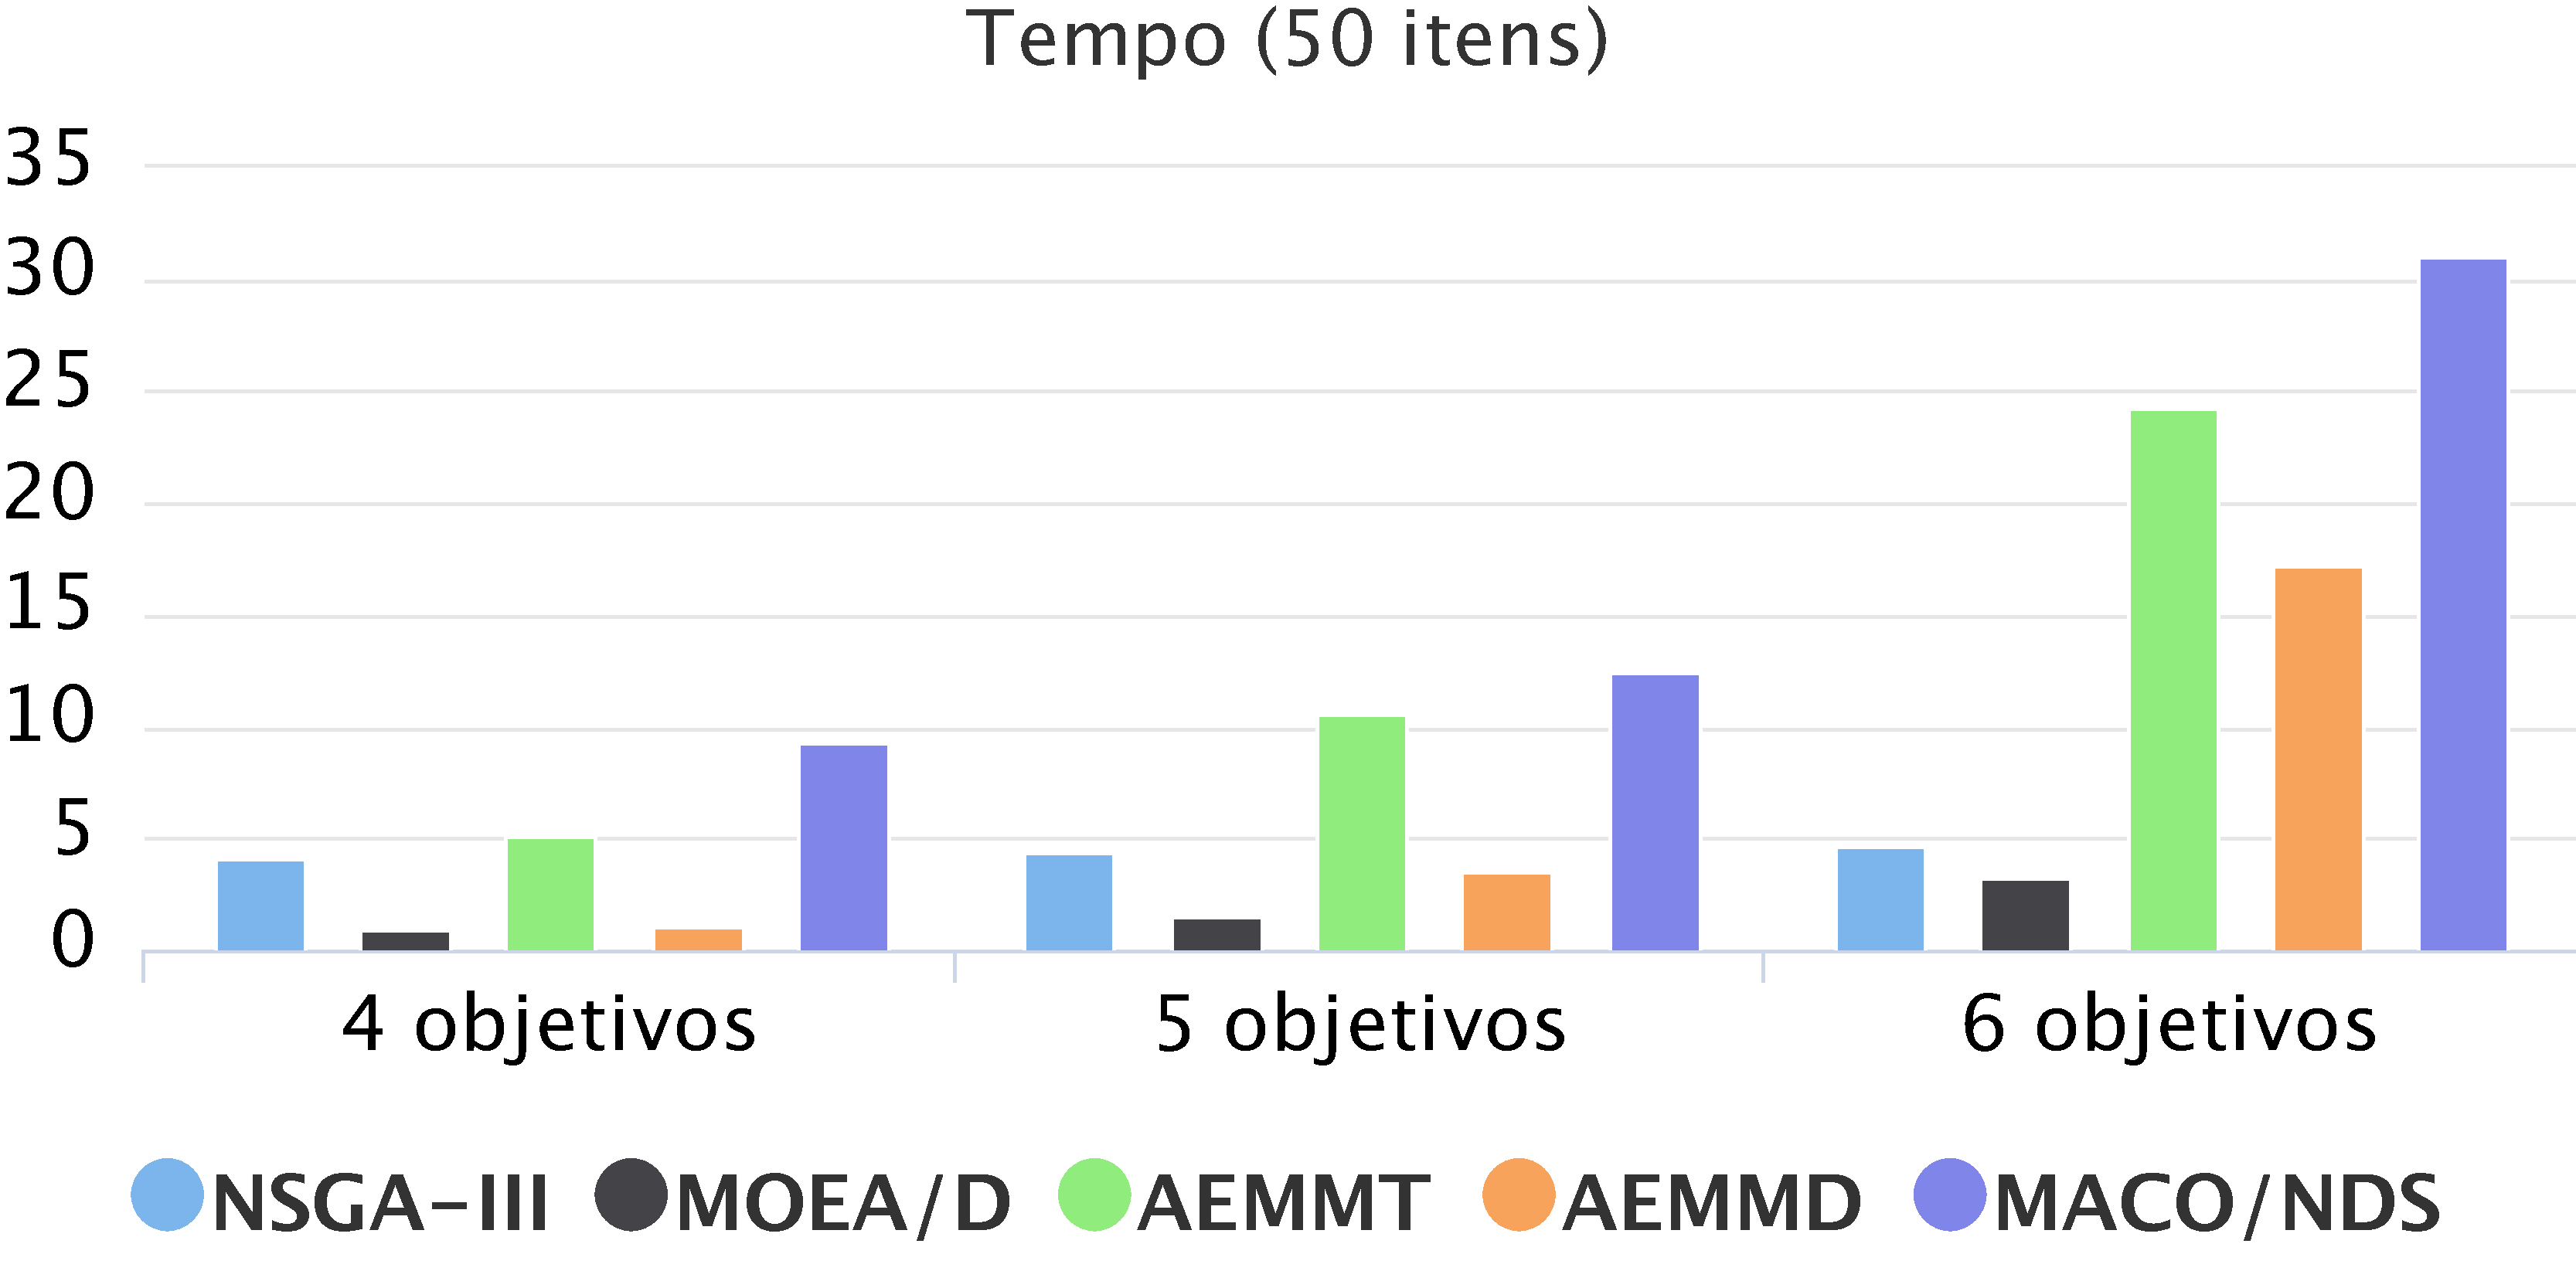
\includegraphics[width=0.5\textwidth]{cap_experimentos/figs/etapa3/time-mkp-50}
	\caption{\label{fig_exp3_pmm_50}Desempenho dos algoritmos na 3ª etapa para o PMM com 50 itens}
\end{figure*}

A \autoref{fig_exp3_pmm_50} mostra o desempenho dos algoritmos no PMM com 50 itens. Como pode ser observado, com exceção do GD, as demais métricas apresentaram um comportamento similar ao das instâncias anteriores. O MACO/NDS e o AEMMT continuam sendo os algoritmos com menores taxas de erro. Enquanto o MACO/NDS consegue menor $ER$ em 4 e 5 objetivos, o AEMMT apresenta melhor resultado em 6 objetivos. O MACO/NDS obtém os melhores valores de $GD$ e $PS$, e o MOEA/D é o algoritmo mais rápido.

\begin{figure*}[!htbp]
	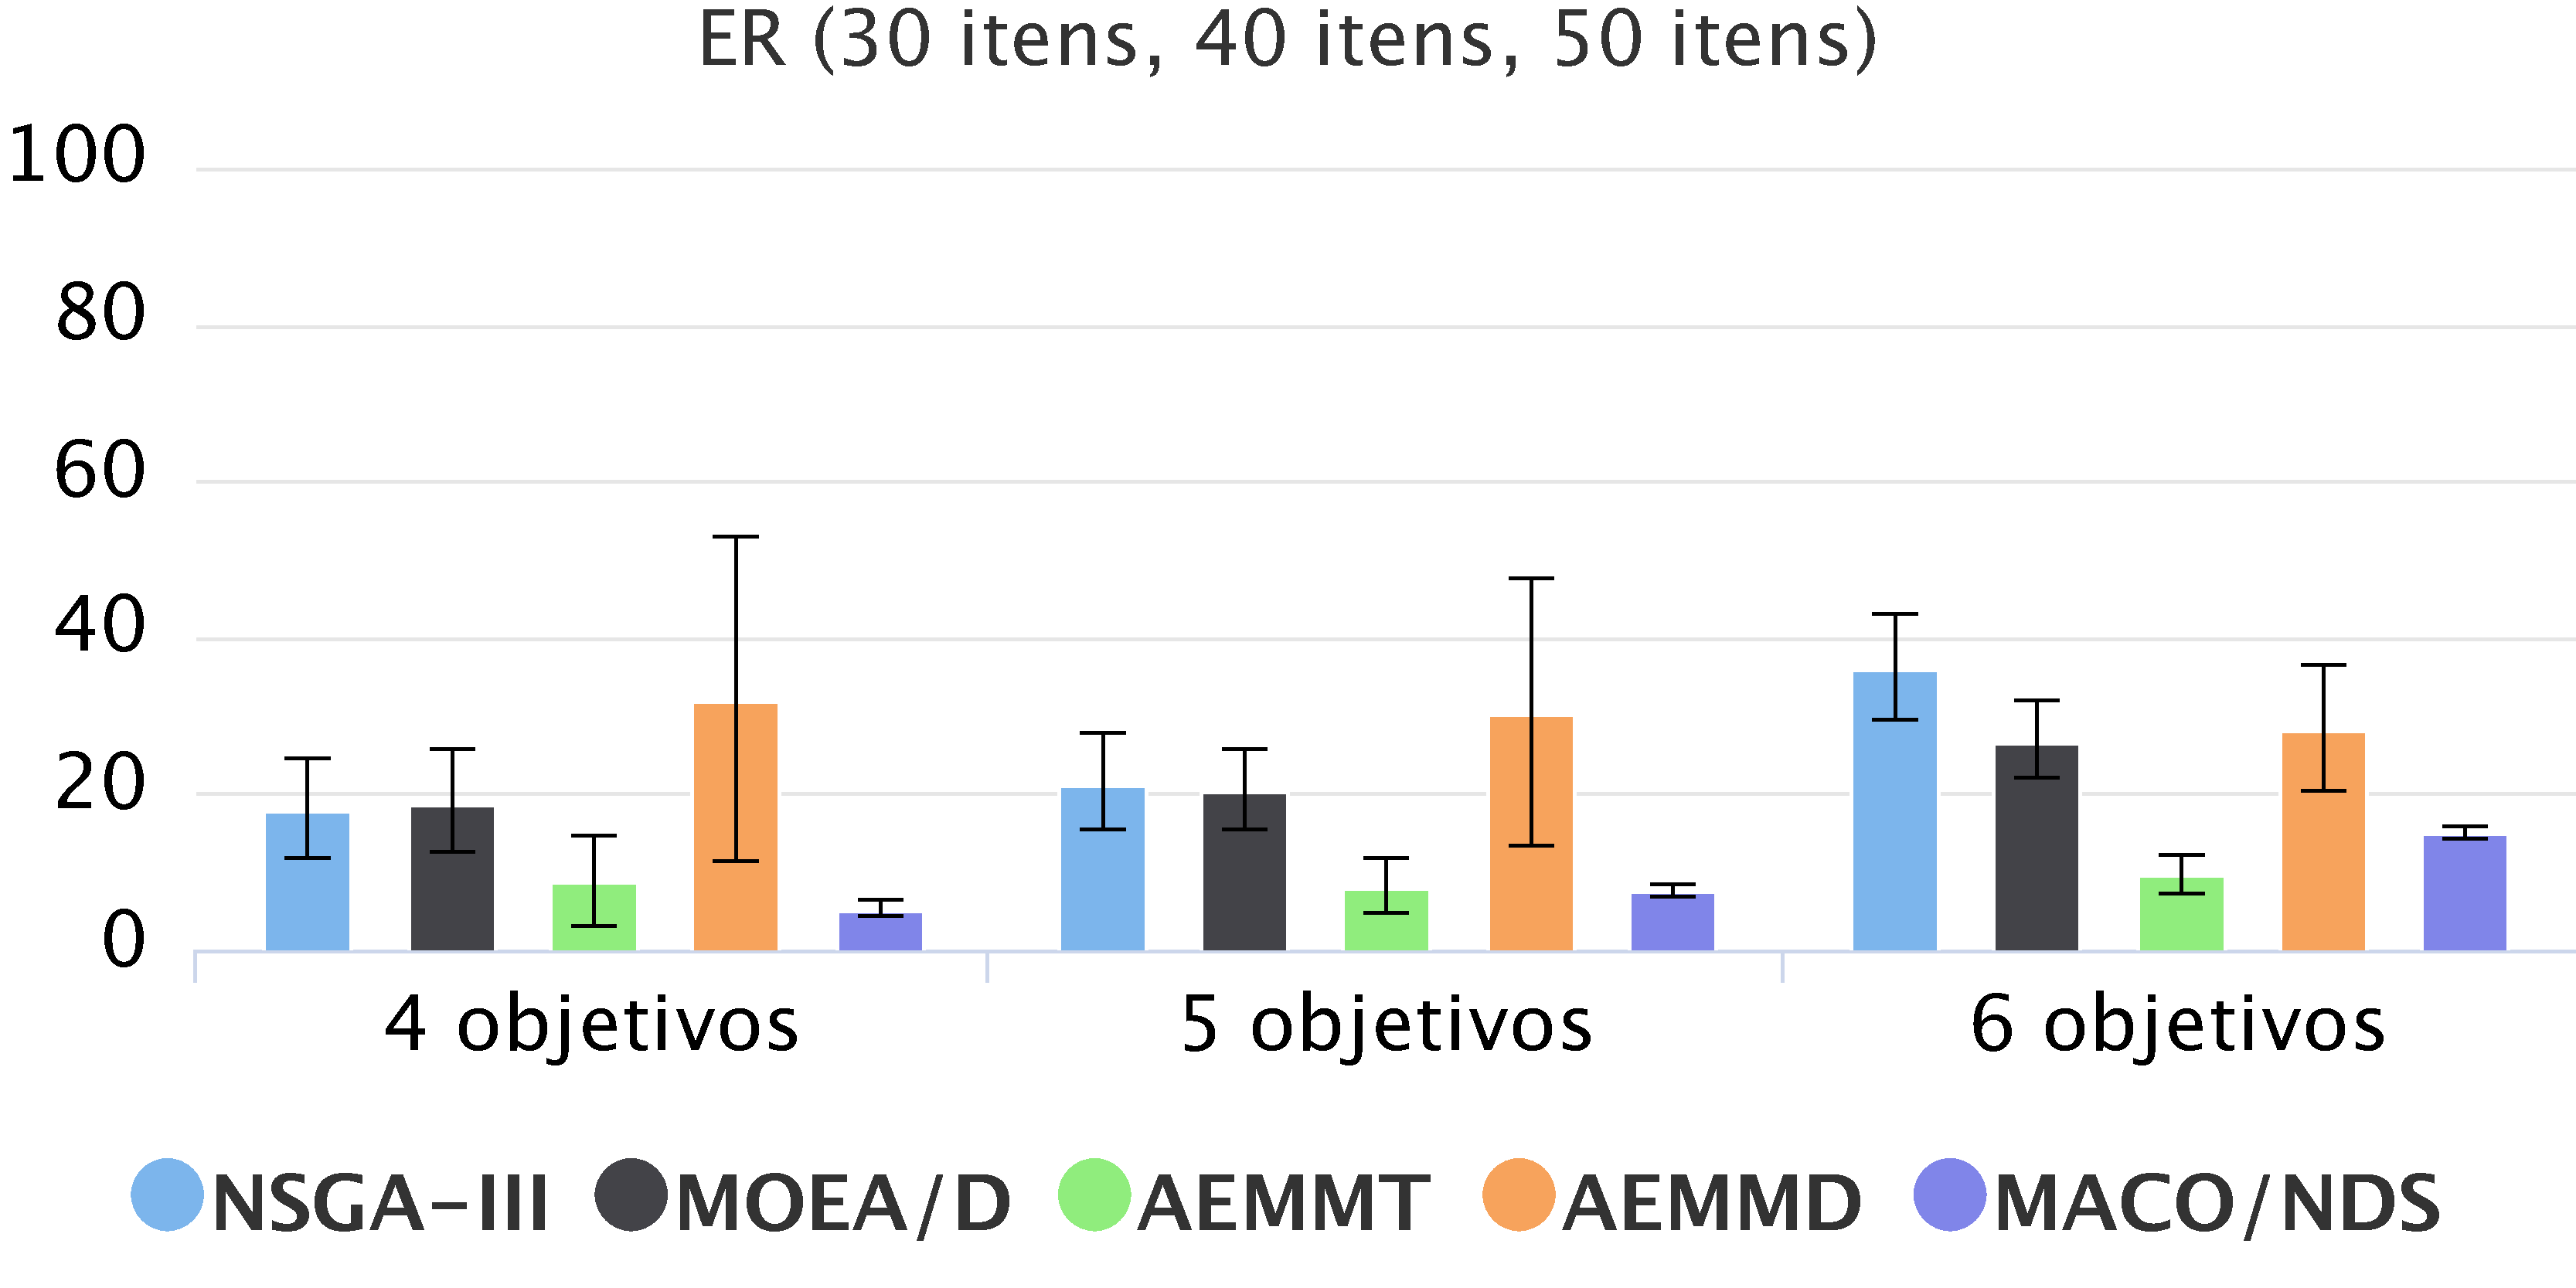
\includegraphics[width=0.5\textwidth]{cap_experimentos/figs/etapa3/er-mkp-todos}
	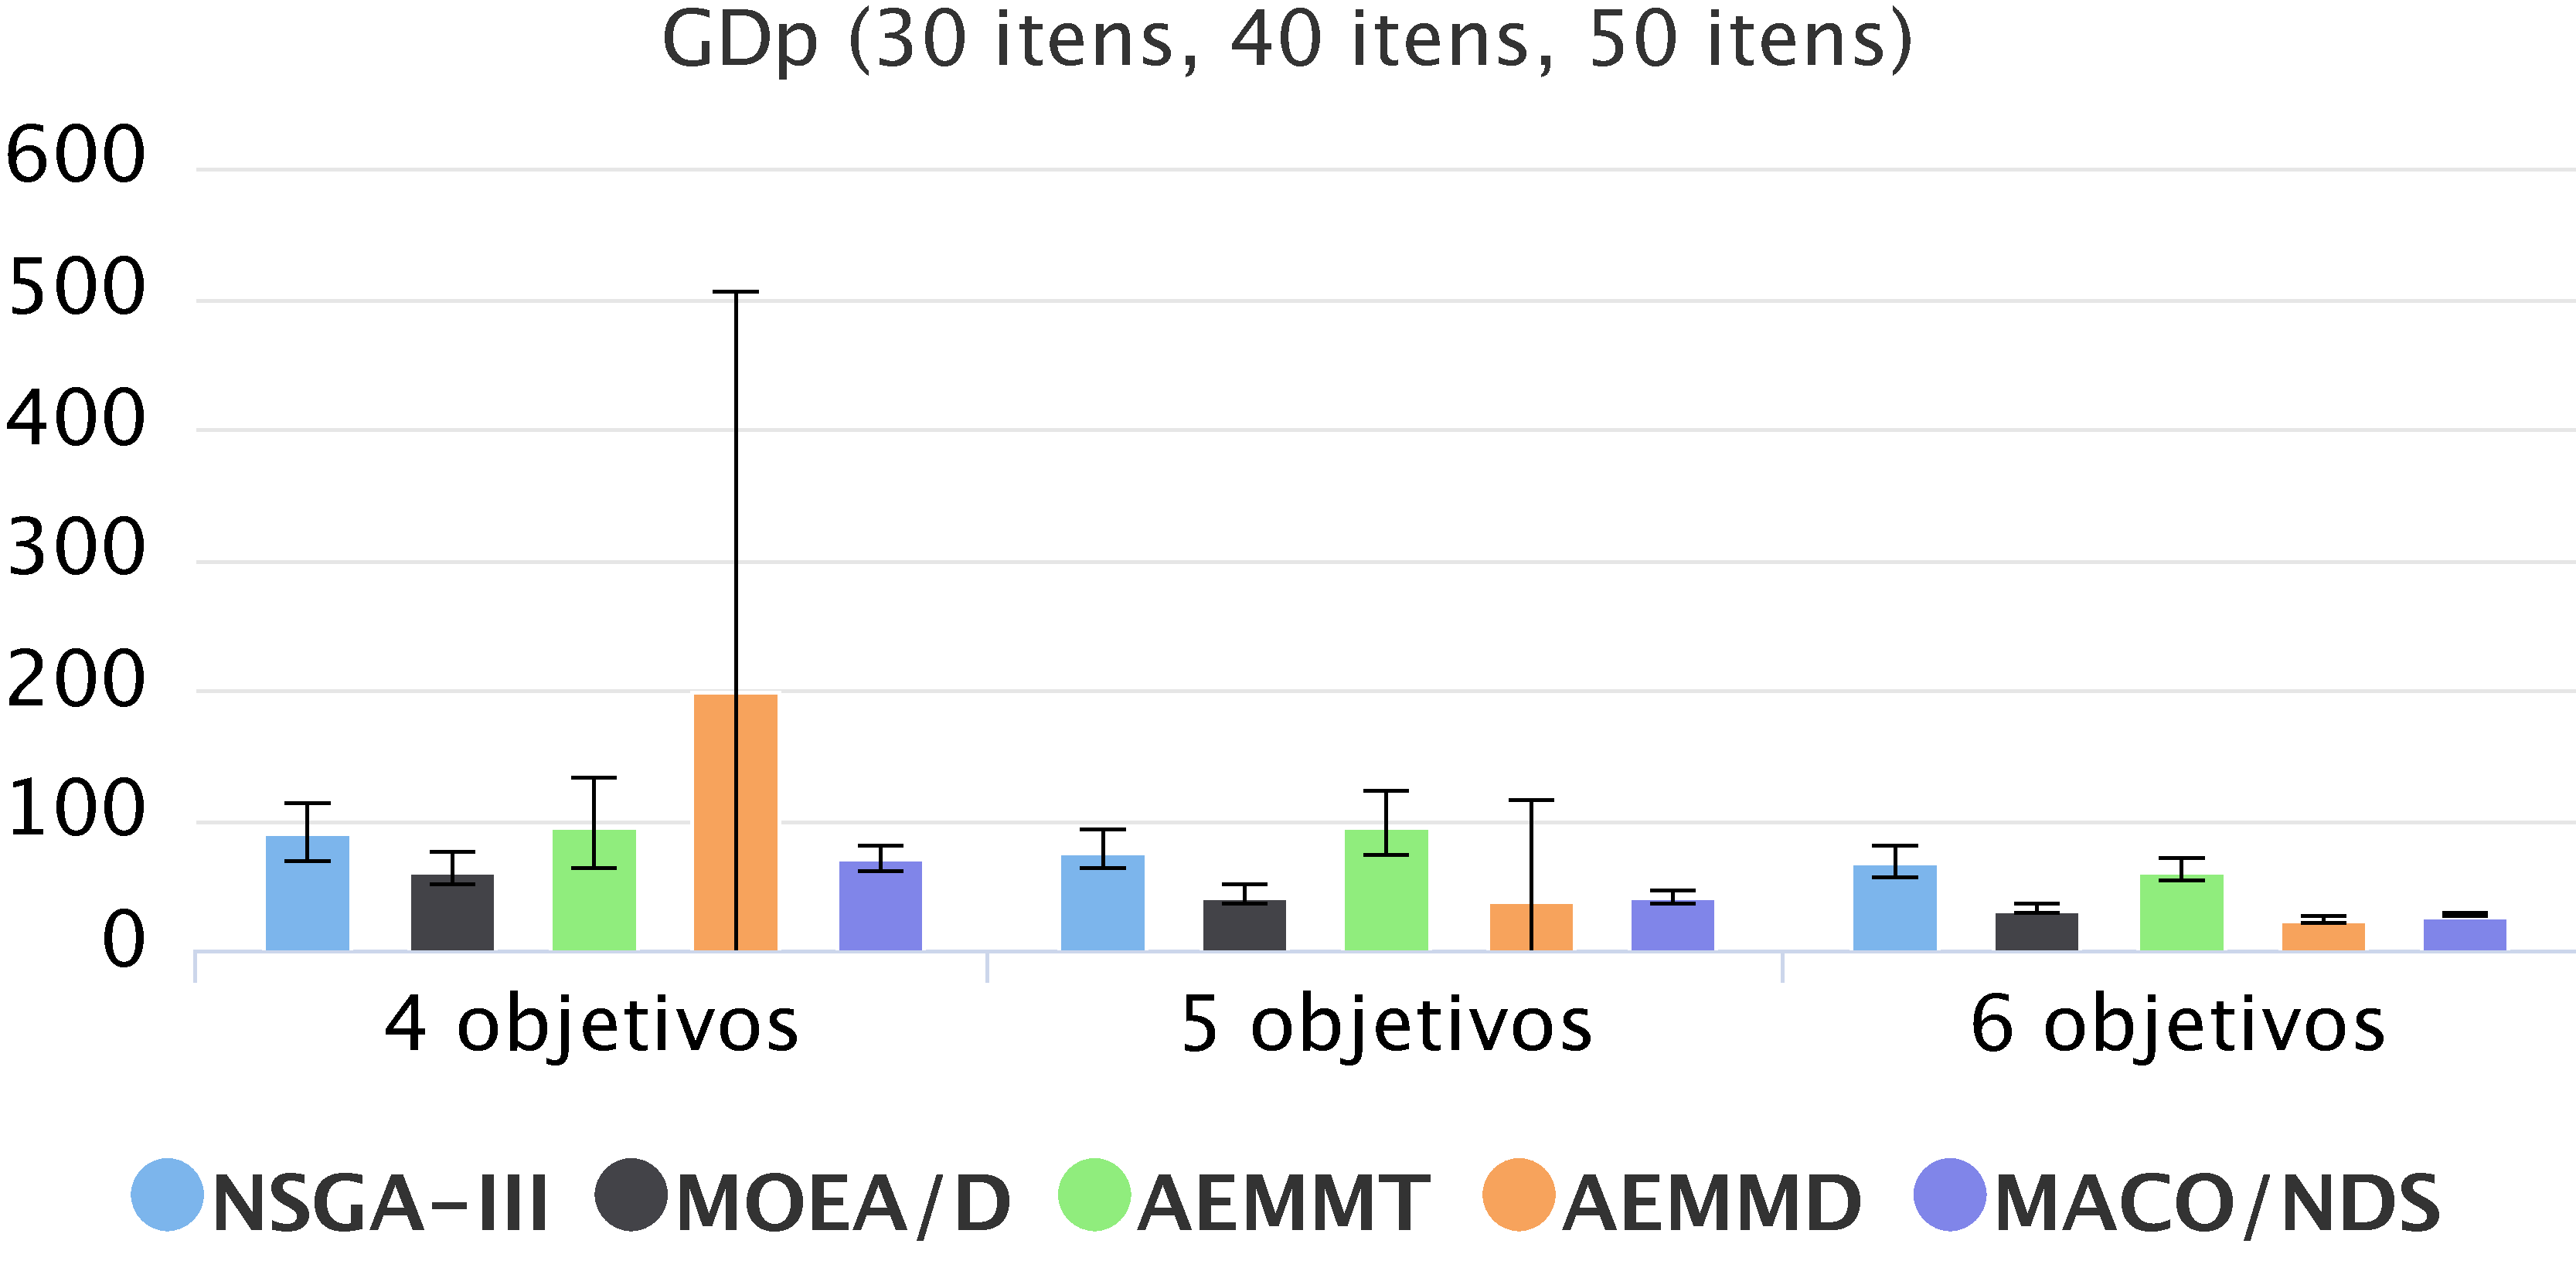
\includegraphics[width=0.5\textwidth]{cap_experimentos/figs/etapa3/gd-mkp-todos}
	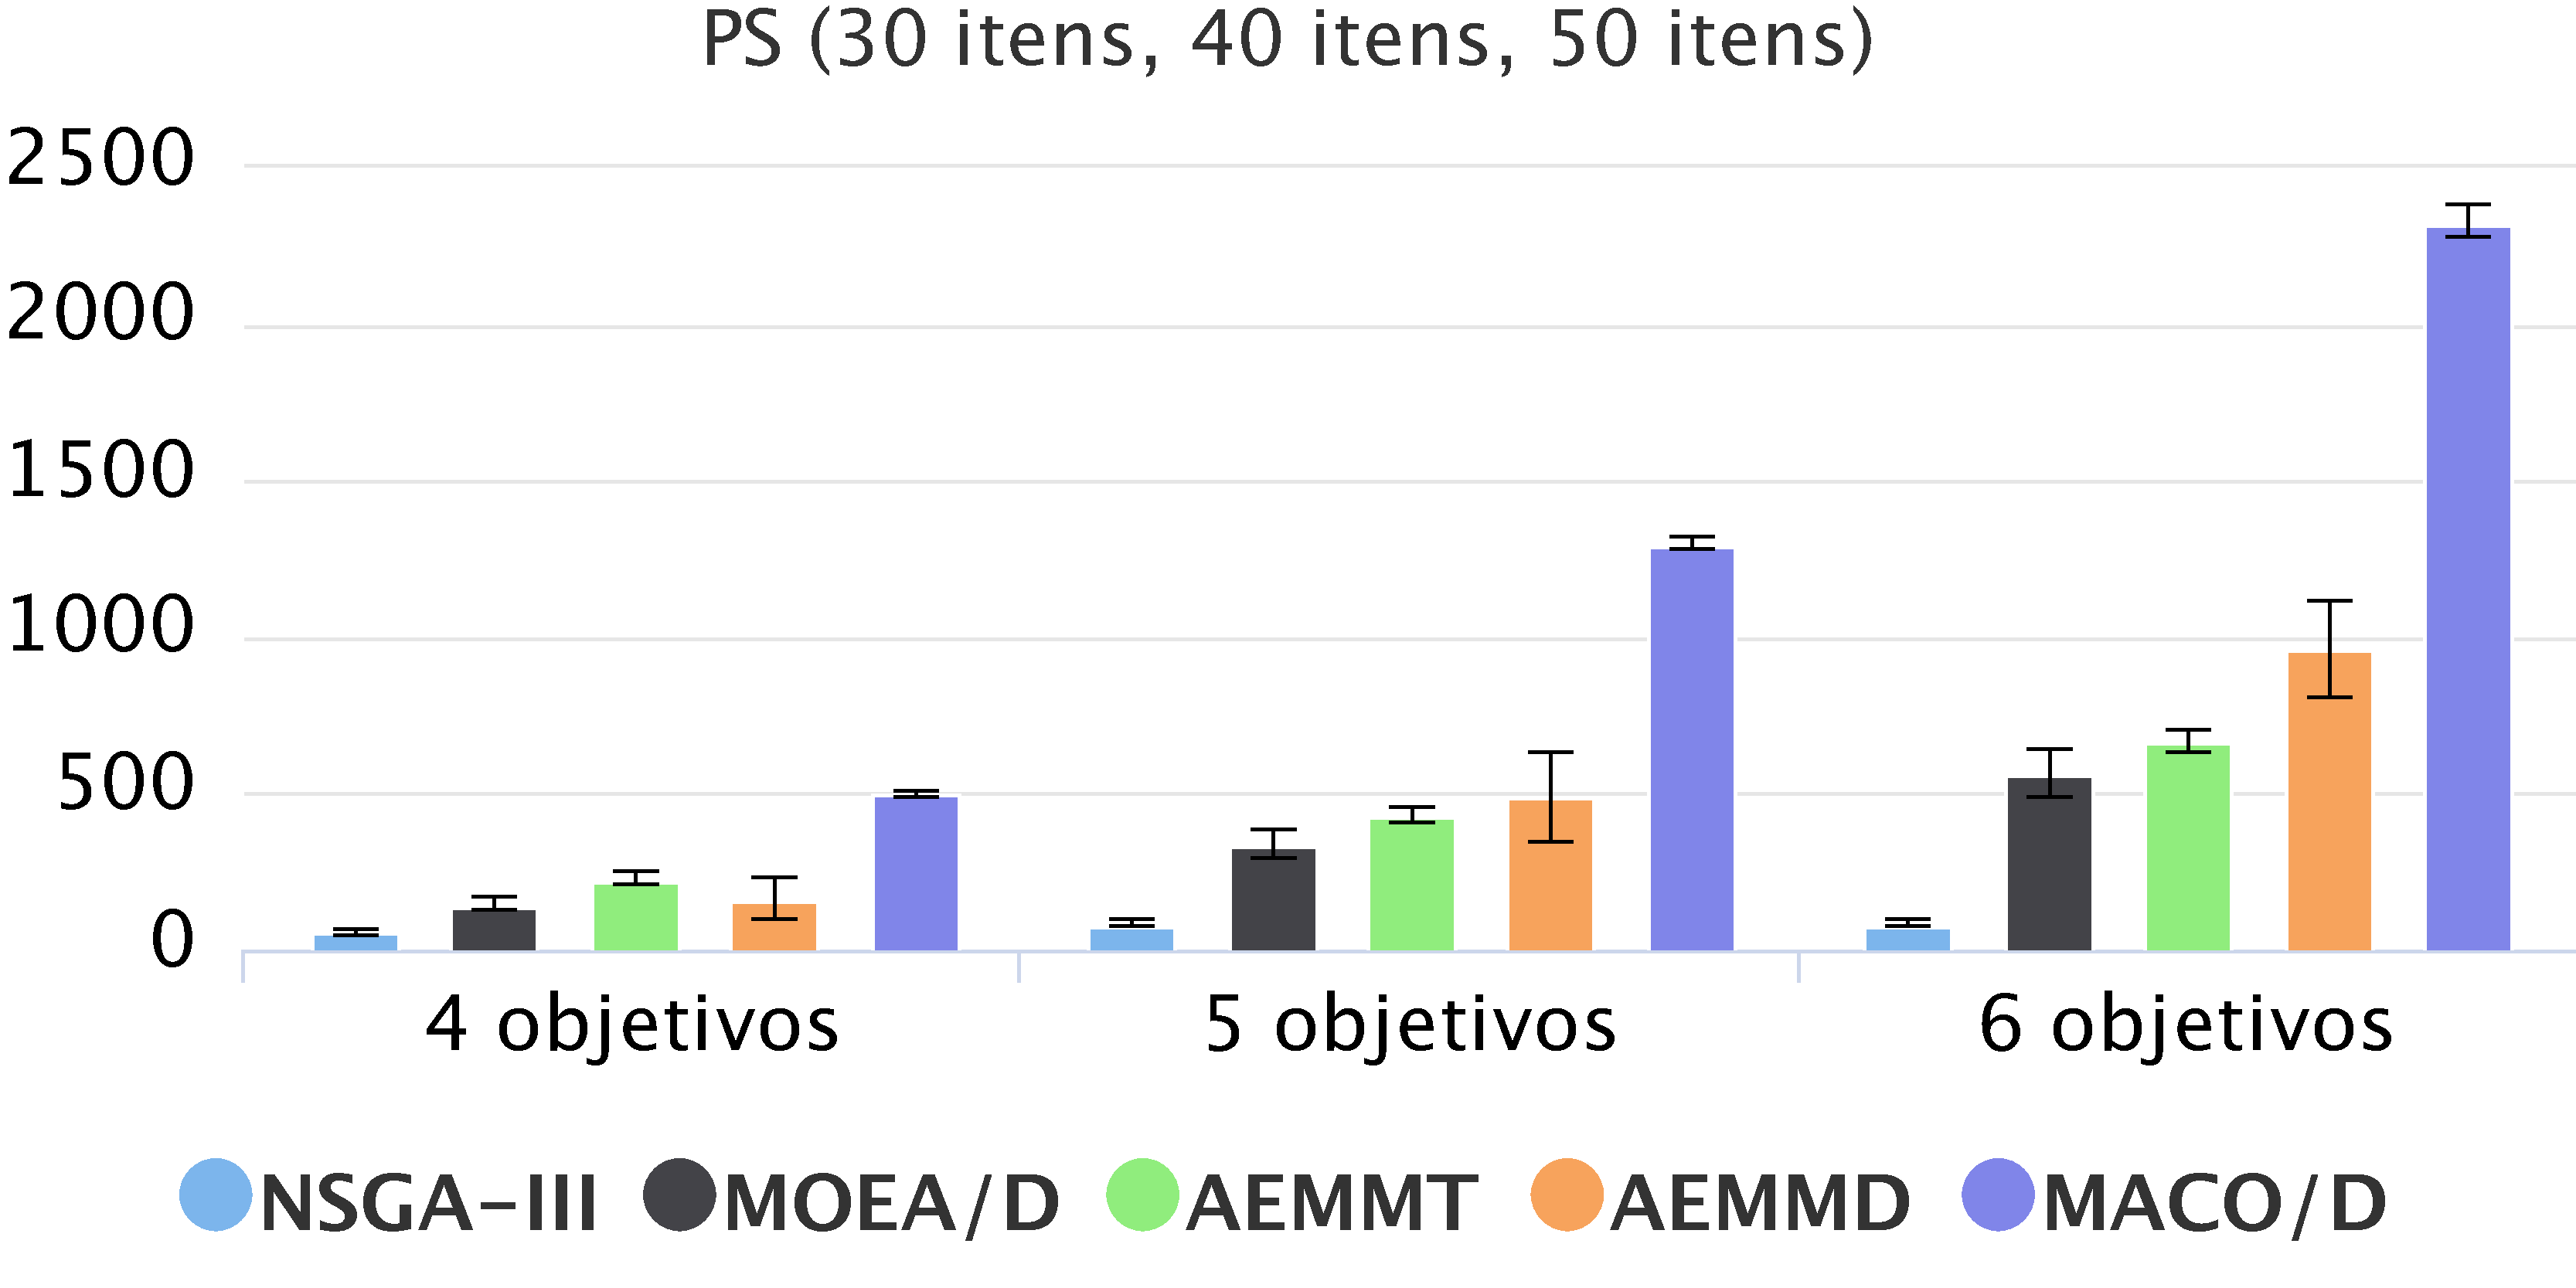
\includegraphics[width=0.5\textwidth]{cap_experimentos/figs/etapa3/ps-mkp-todos}
	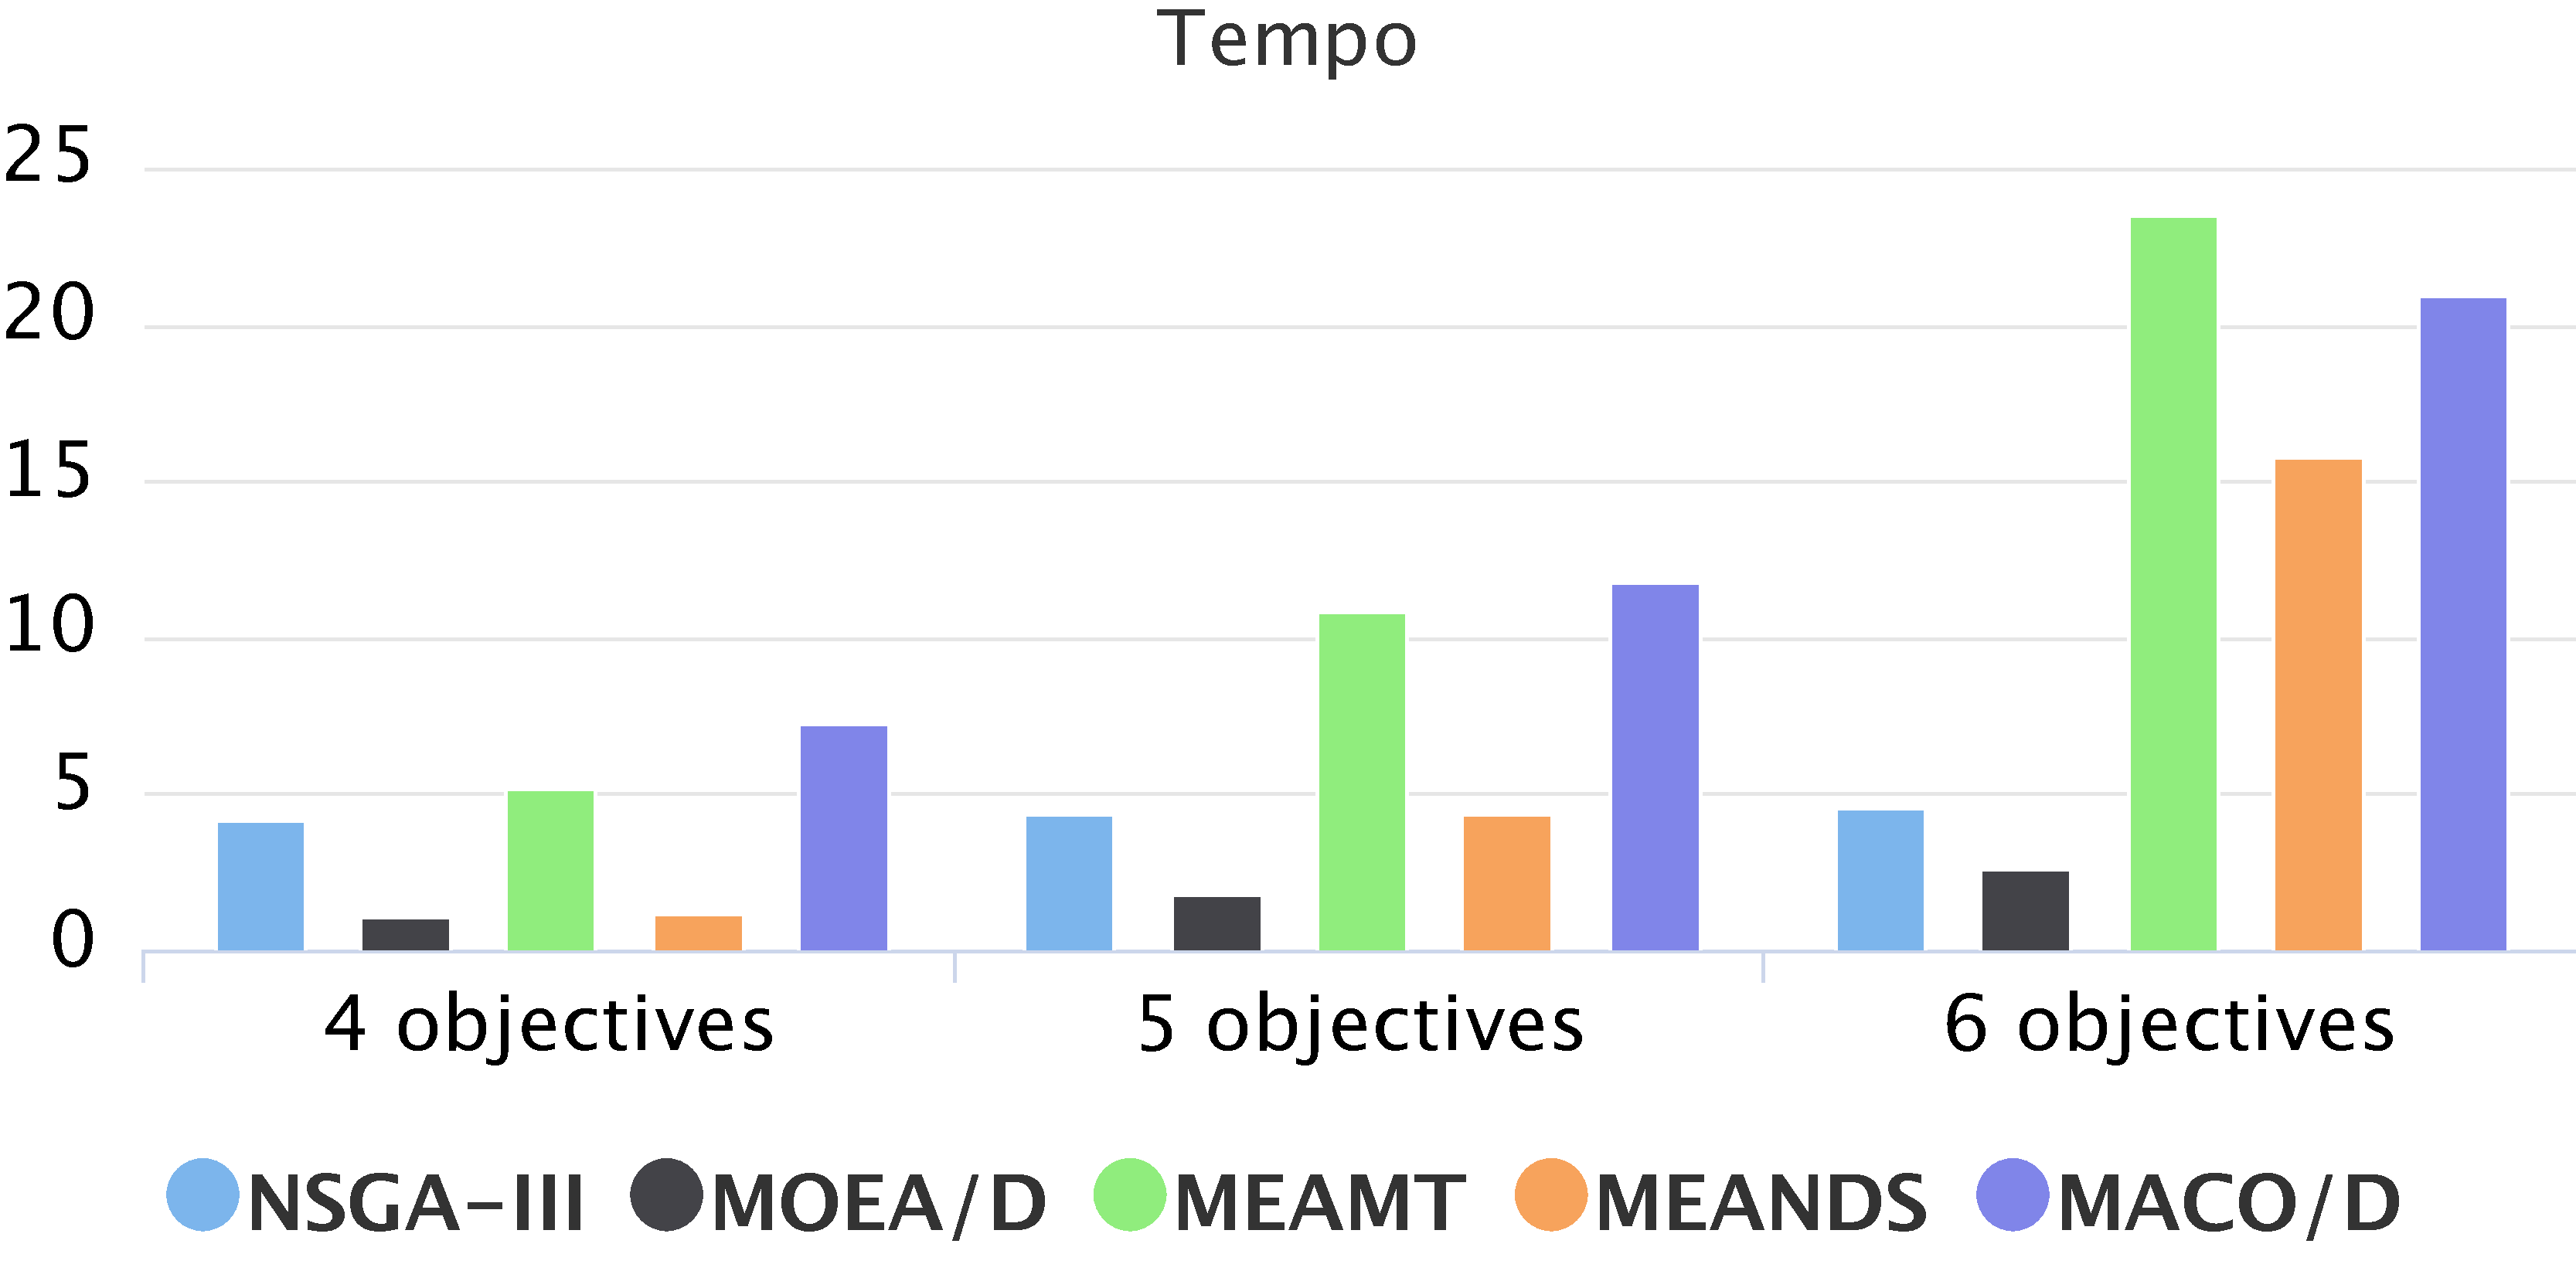
\includegraphics[width=0.5\textwidth]{cap_experimentos/figs/etapa3/time-mkp-todos}
	\caption{\label{fig_exp3_pmm_todos}Resultado consolidado da 3ª etapa considerando o PMM com 30, 40 e 50 itens}
\end{figure*}

A fim de se fazer uma análise geral dos resultados, a média entre os 3 cenários é apresentada nos gráficos da \autoref{fig_exp3_pmm_todos}. As taxas de erro são muito baixas para o AEMMT e o MACO/NDS, quando comparados aos demais algoritmos. Os resultados em $GD$ são bons para a maioria dos métodos. Apenas o AEMMD apresenta um valor alto de GD e com elevado desvio padrão para o problema de 4 objetivos. O MOEA/D produz o melhor $GD$ no problema de 4 objetivos, enquanto que, para 5 e 6 objetivos, o MACO/NDS e o AEMMD consegue valores bem similares. É importante notar que os desvio padrões no AEMMD são altos, representando uma certa instabilidade do algoritmo em gerar boas soluções. Em termos da cobertura da fronteira de Pareto ($PS$), o MACO/D alcançou os melhores valores em todas as formulações de objetivos. Analisando o tempo de execução médio, o AEMMT, o AEMMD e o MACO/S variam bastante com o número de objetivos, enquanto os demais são estáveis. O MOEA/D é o algoritmo mais rápido entre os avaliados nesta etapa dos experimentos.

\begin{figure*}[!htbp]
	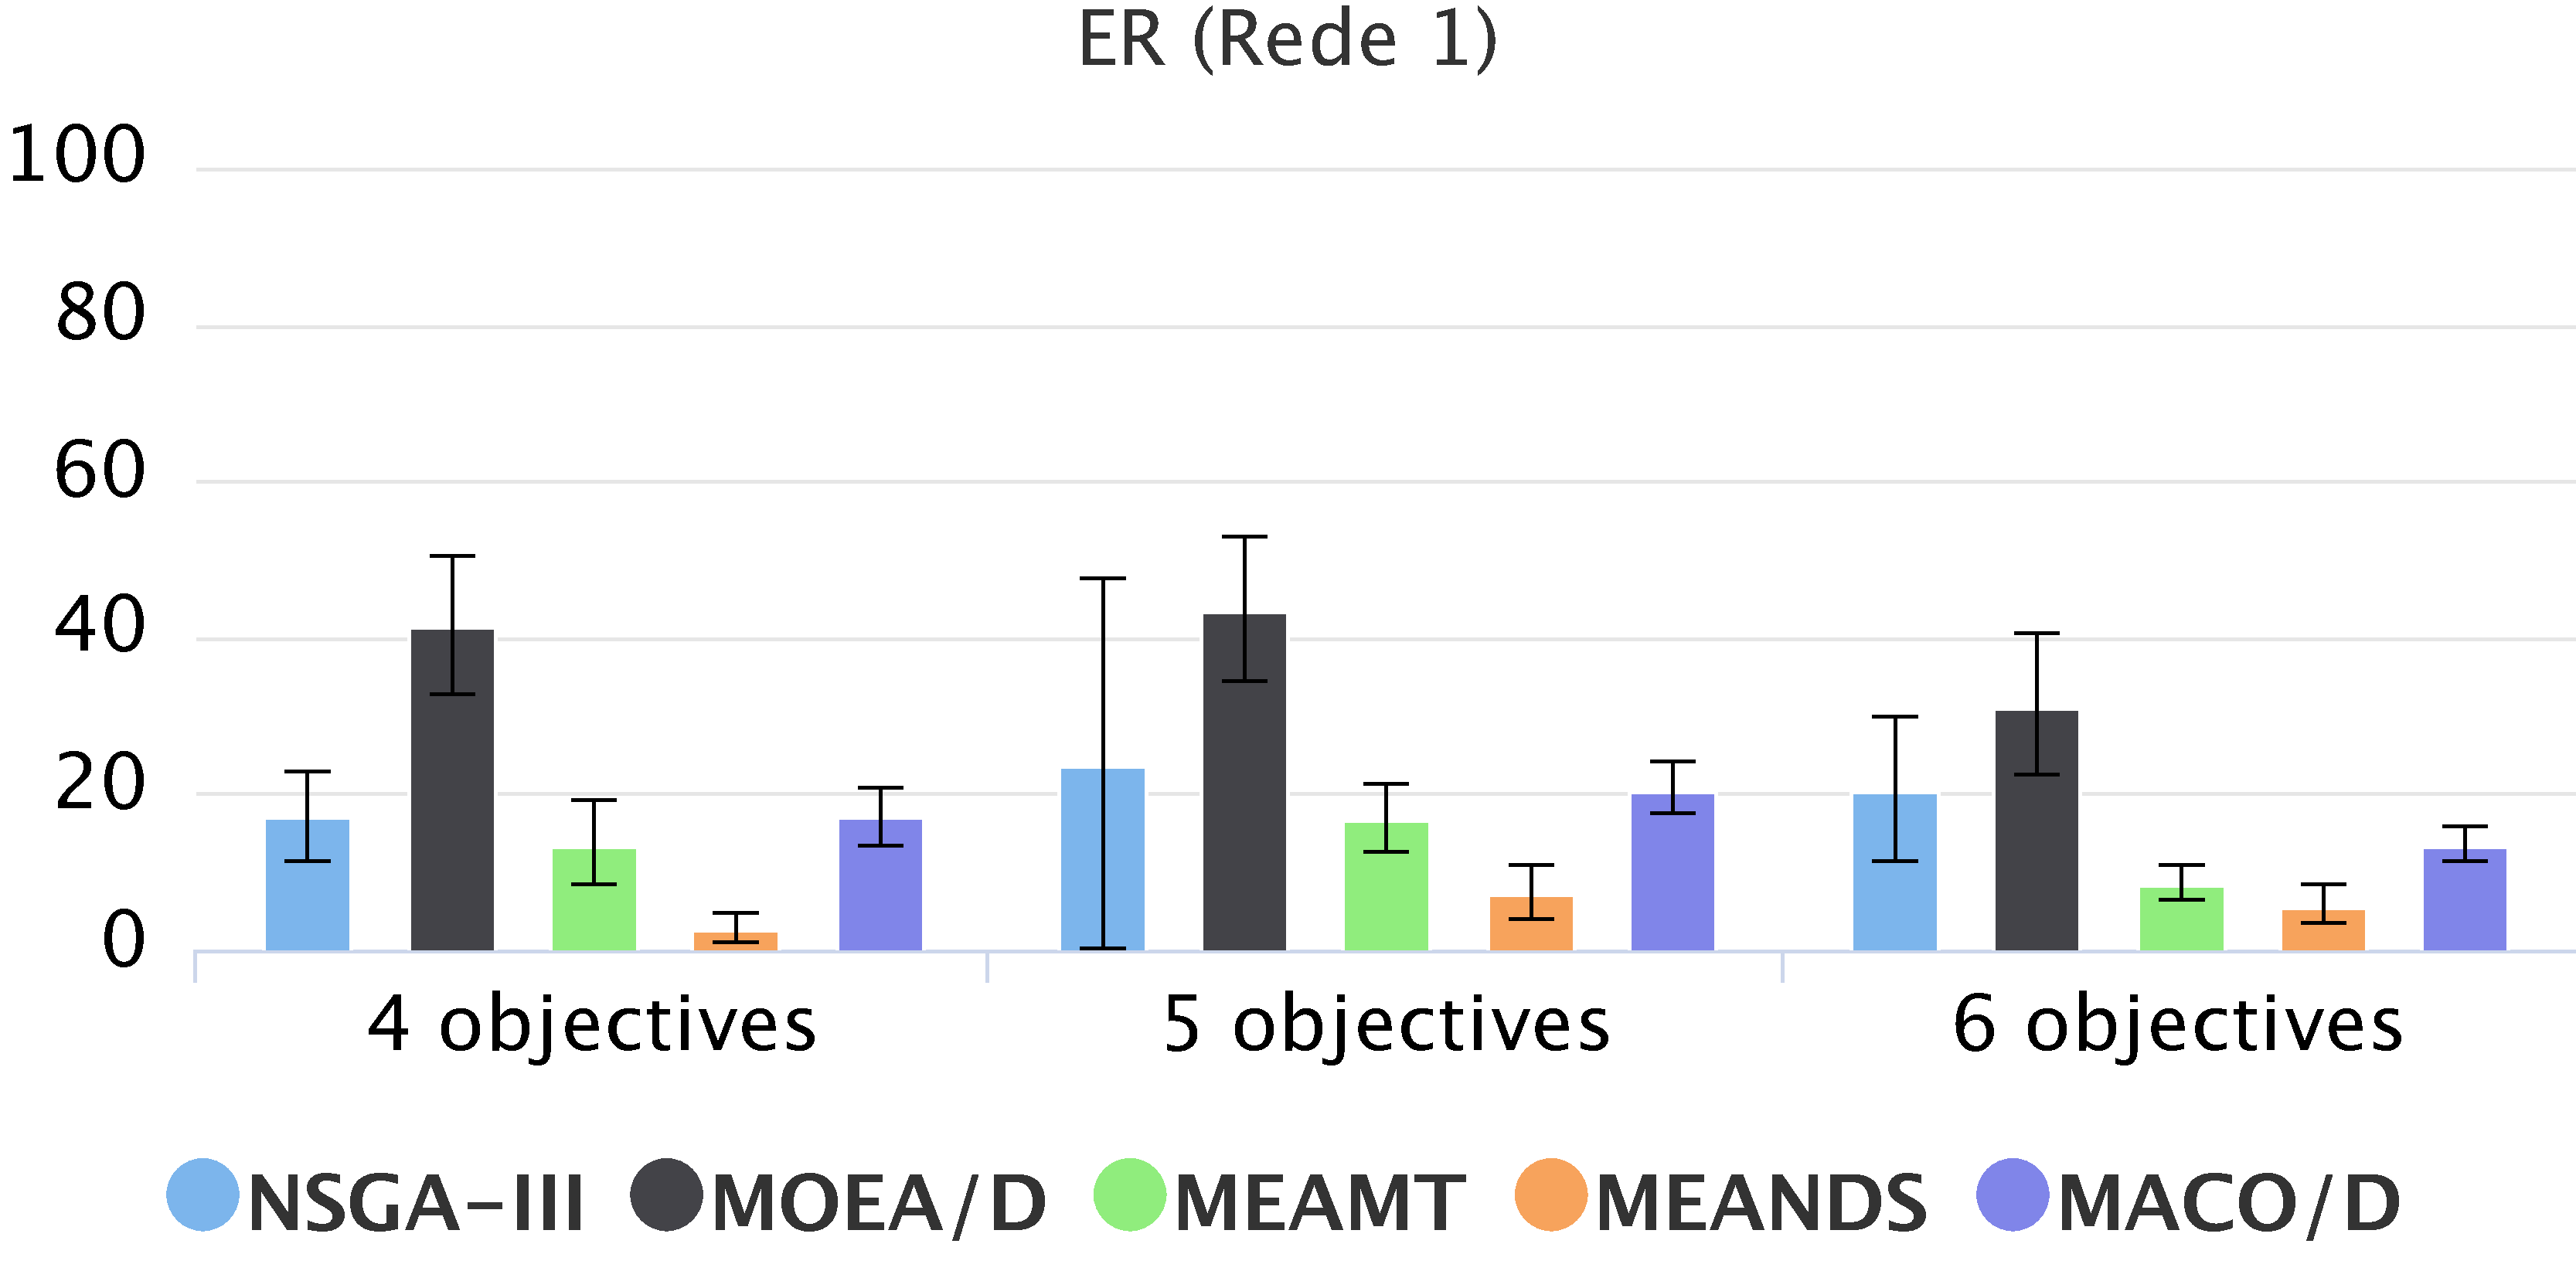
\includegraphics[width=0.5\textwidth]{cap_experimentos/figs/etapa3/er-mrp-r1}
	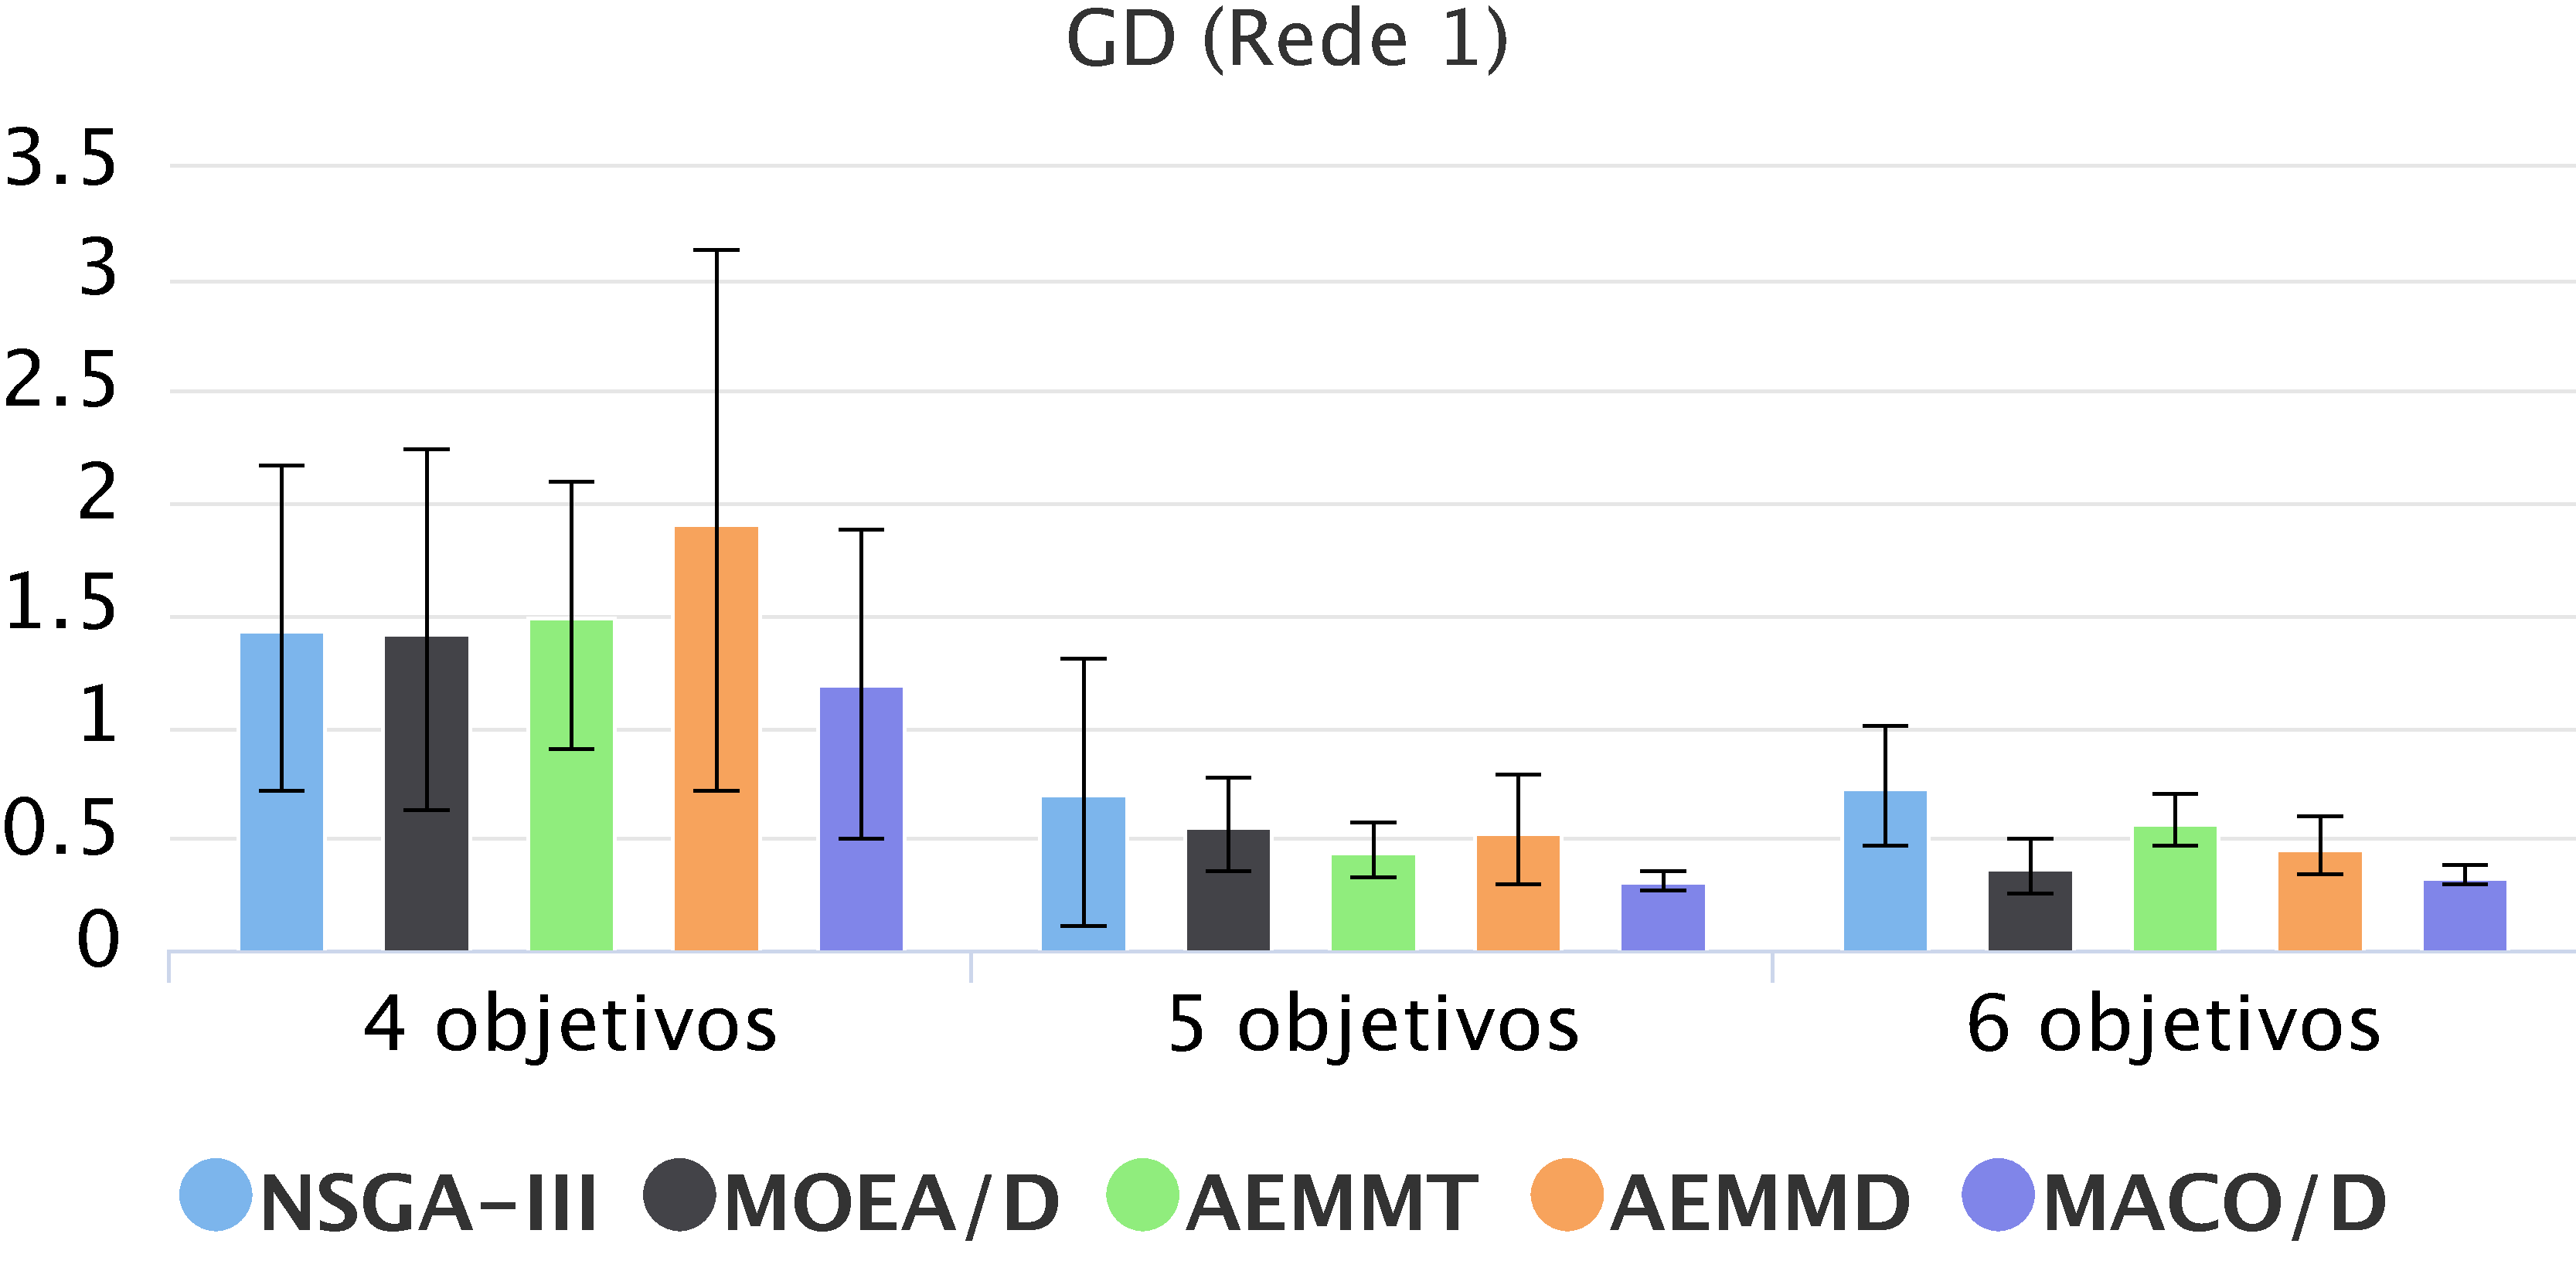
\includegraphics[width=0.5\textwidth]{cap_experimentos/figs/etapa3/gd-mrp-r1}
	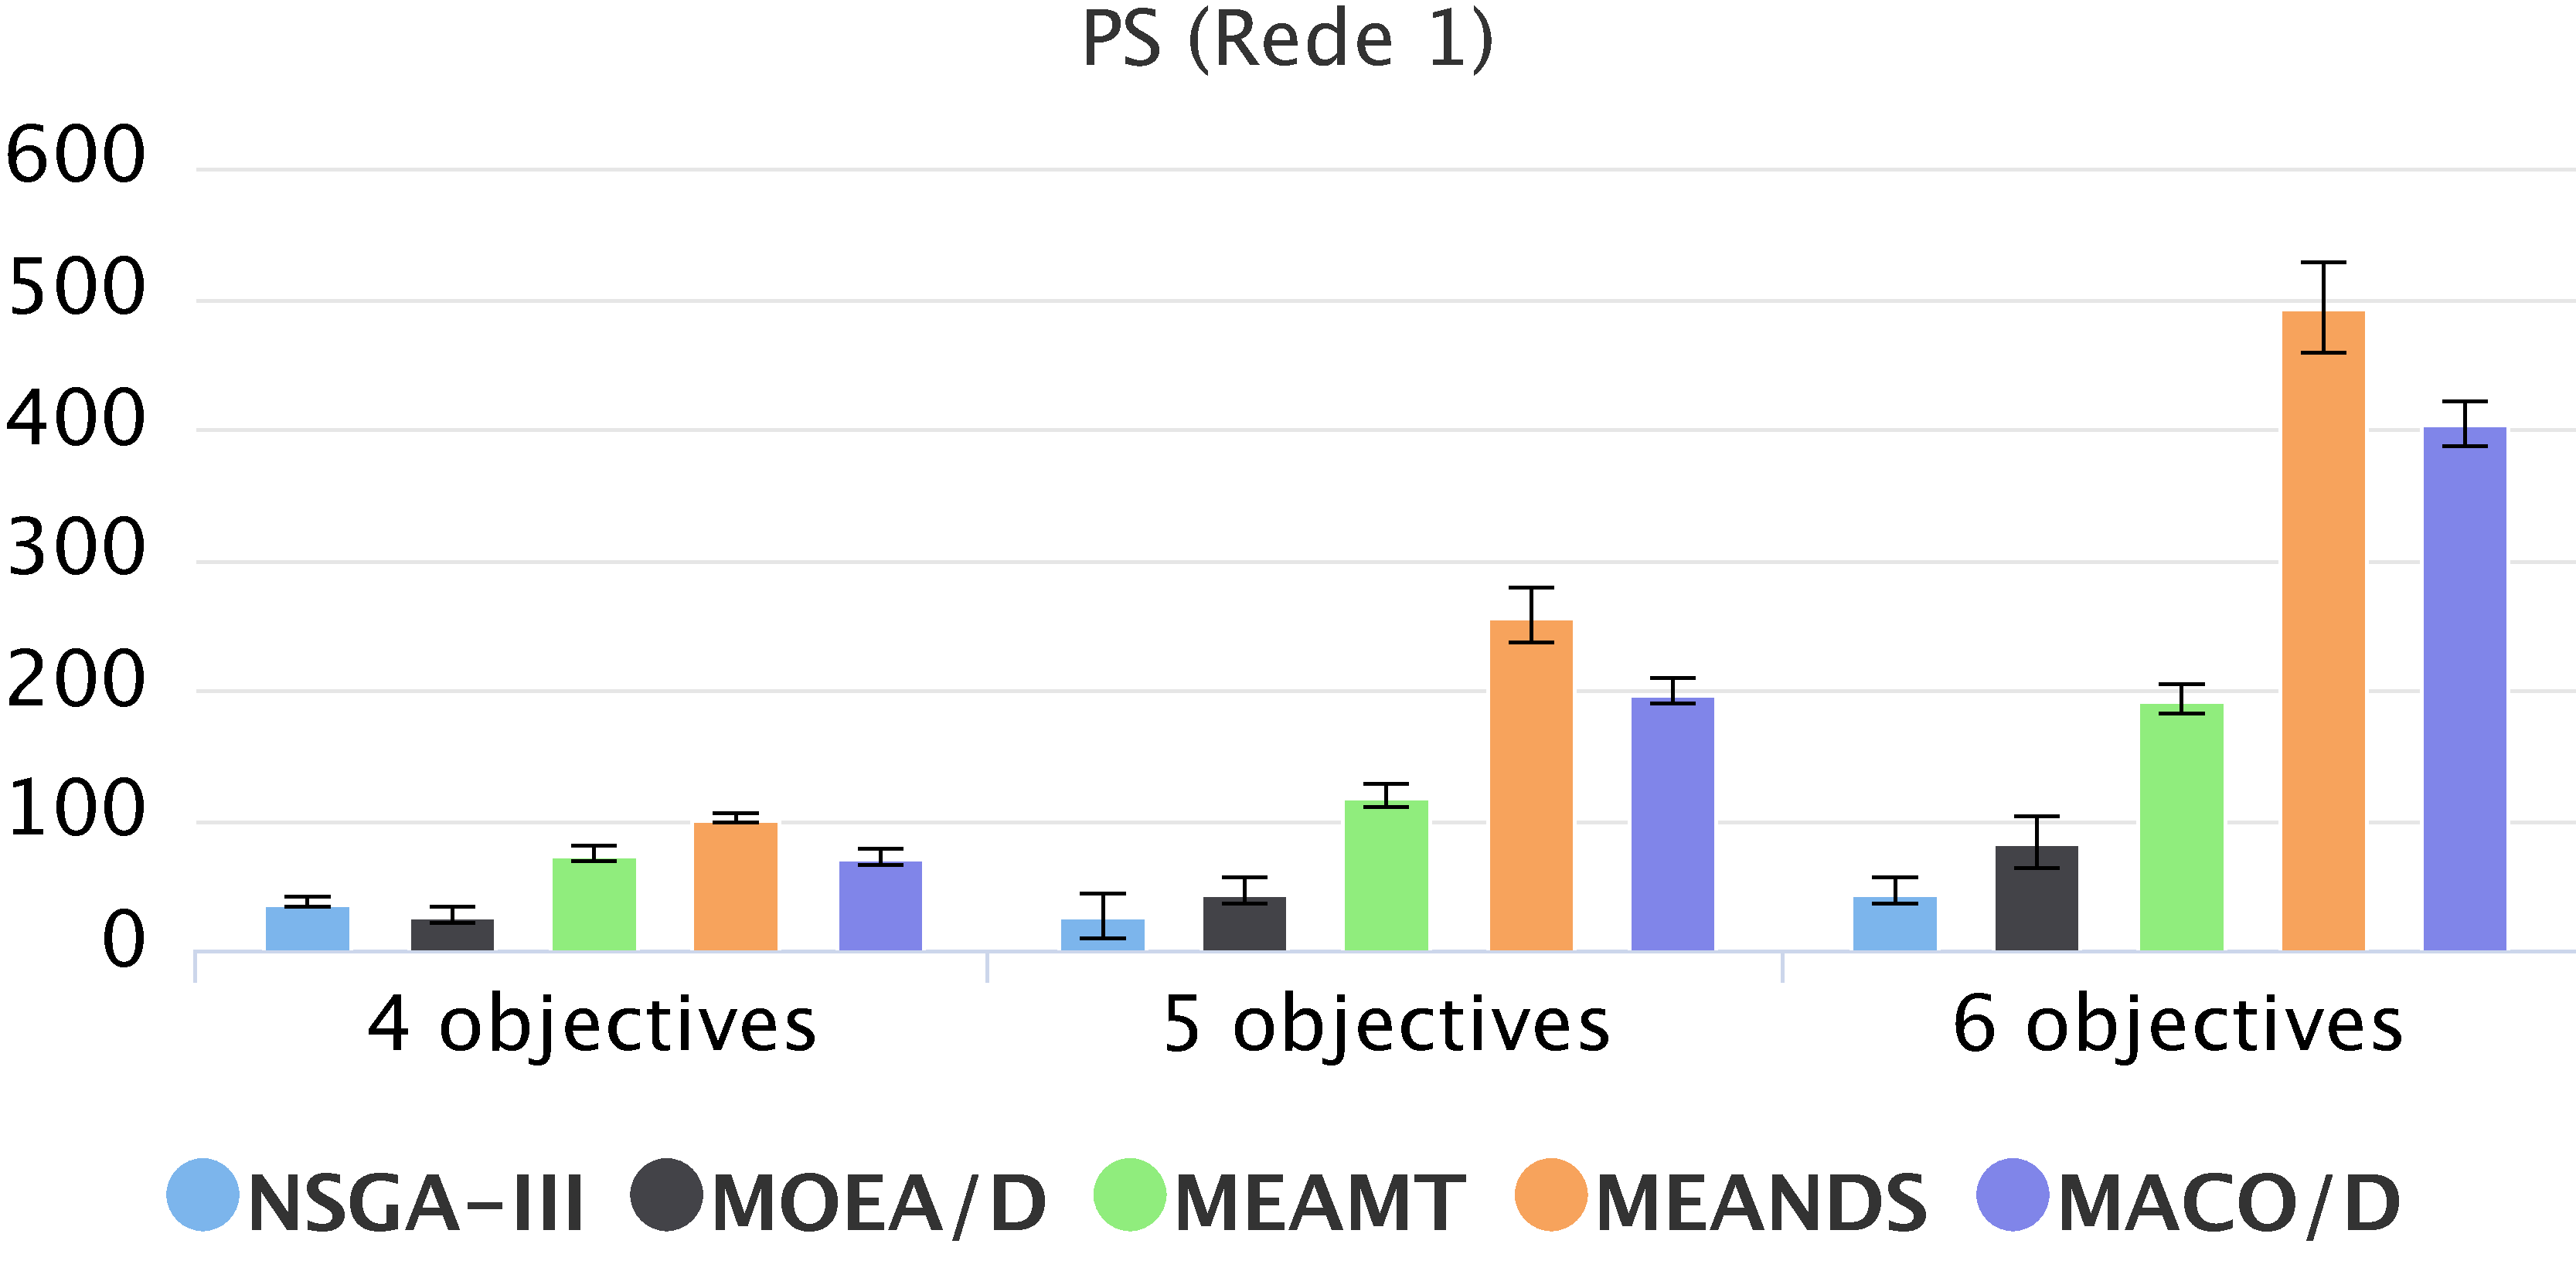
\includegraphics[width=0.5\textwidth]{cap_experimentos/figs/etapa3/ps-mrp-r1}
	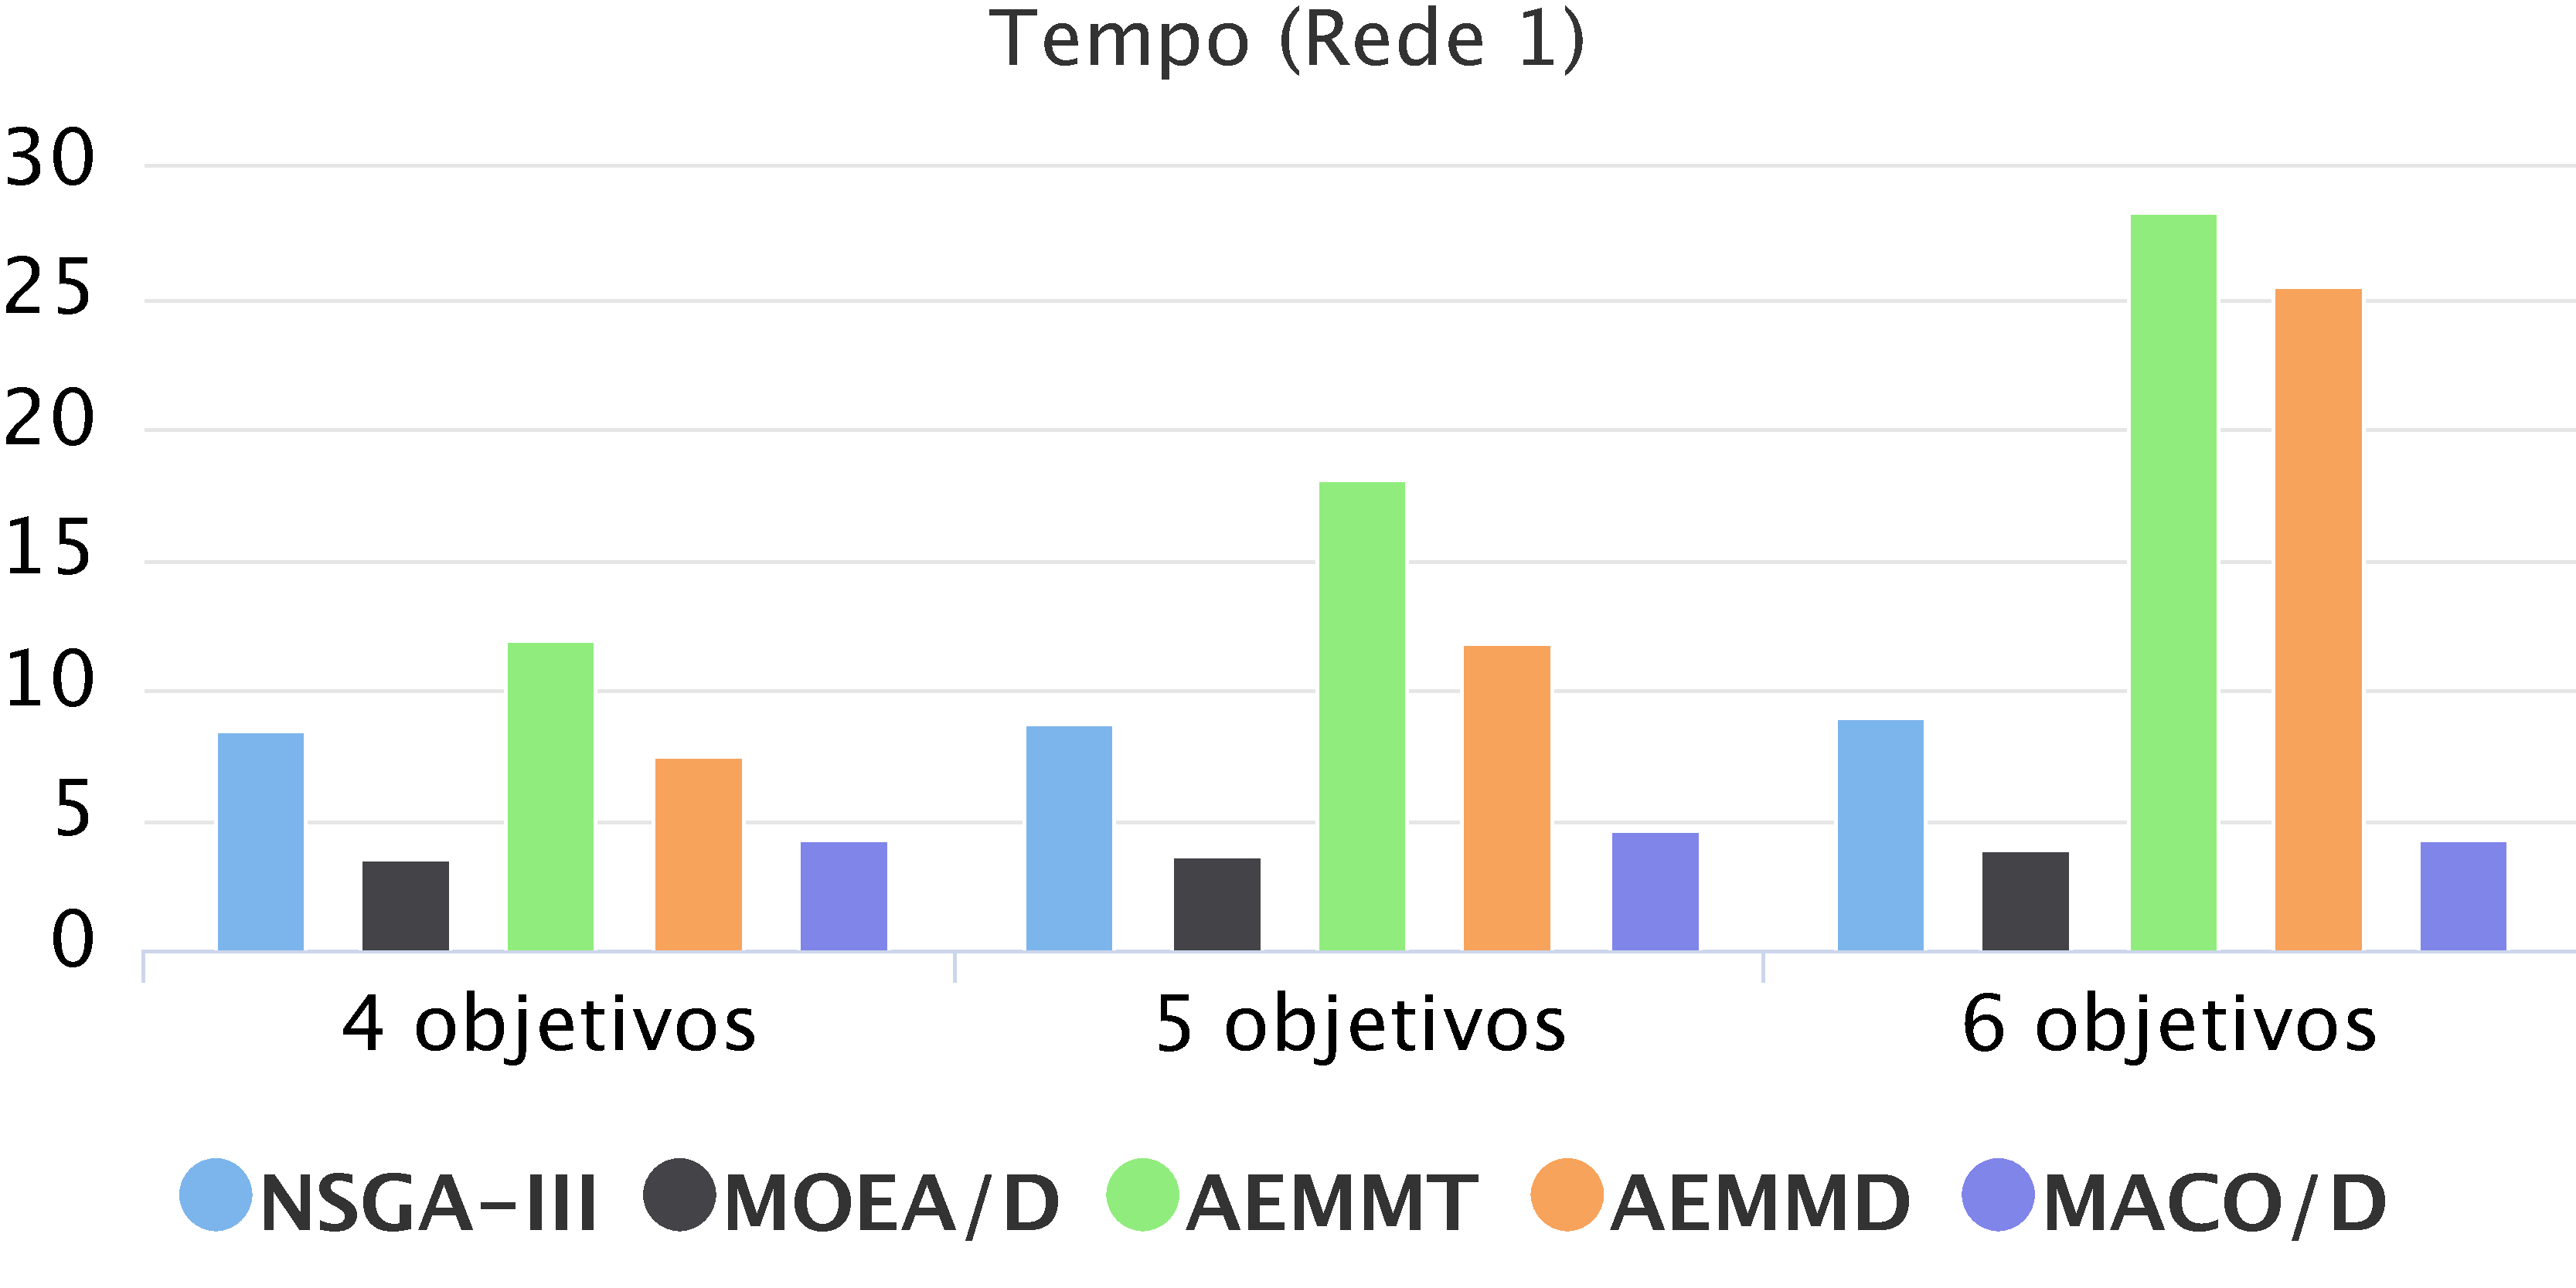
\includegraphics[width=0.5\textwidth]{cap_experimentos/figs/etapa3/time-mrp-r1}
	\caption{\label{fig_exp3_prm_r1}Desempenho dos algoritmos na 3ª etapa para o PRM na rede 1}
\end{figure*}

Os gráficos correspondentes ao PRM na rede 1 são apresentados na \autoref{fig_exp3_prm_r1}. Em relação à taxa de erro, o AEMMD obtém os menores valores em todas as formulações de objetivos. Em seguida, aparecem o AEMMT e o MACO/D, respectivamente, mas com valores próximos. Por fim, os piores valores de ER foram obtidos pelo NSGA-III e pelo MOEA/D. Com relação ao $GD$, é possível observar que o MACO/NDS e o MOEA/D atingem desempenhos bem próximos, sendo o MACO/NDS o melhor entre os dois. Considerando o tamanho das fronteiras de Pareto encontrada ($PS$), o AEMMD é o melhor algoritmo, seguido pelo MACO/NDS, AEMMT, MOEA/D e NSGA-III, nessa ordem. O MACO/NDS e o MOEA/D são os algoritmos mais rápidos, enquanto o AEMMT e o AEMMD são os mais lentos.

\begin{figure*}[!htbp]	
	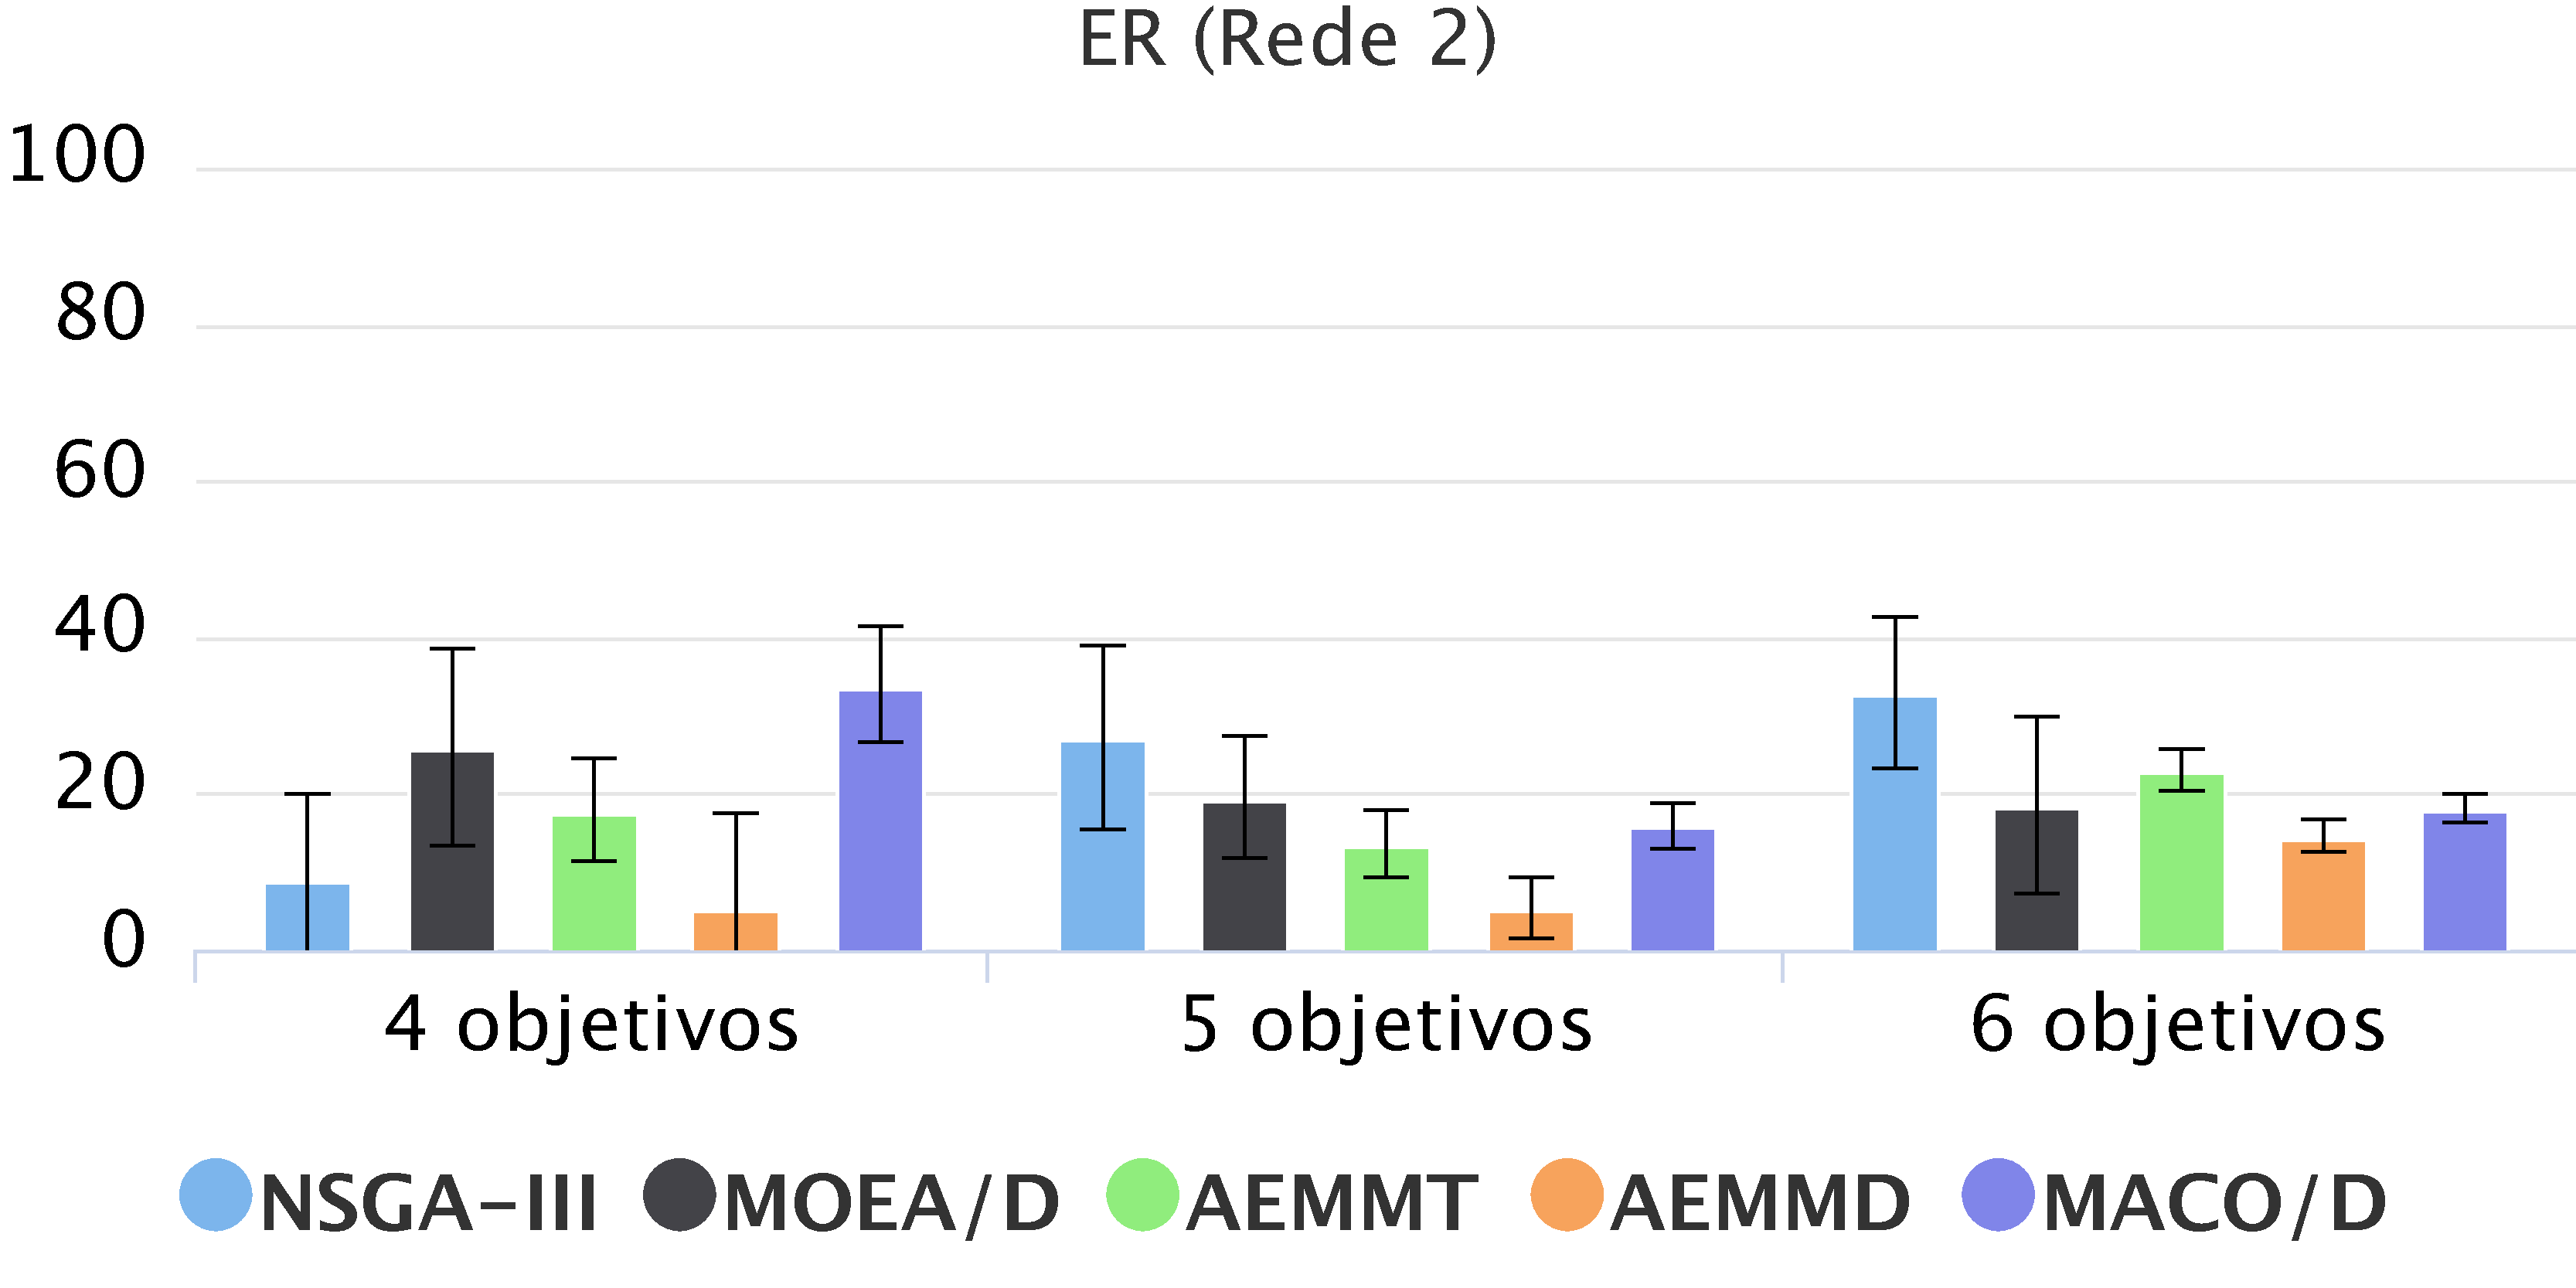
\includegraphics[width=0.5\textwidth]{cap_experimentos/figs/etapa3/er-mrp-r2}
	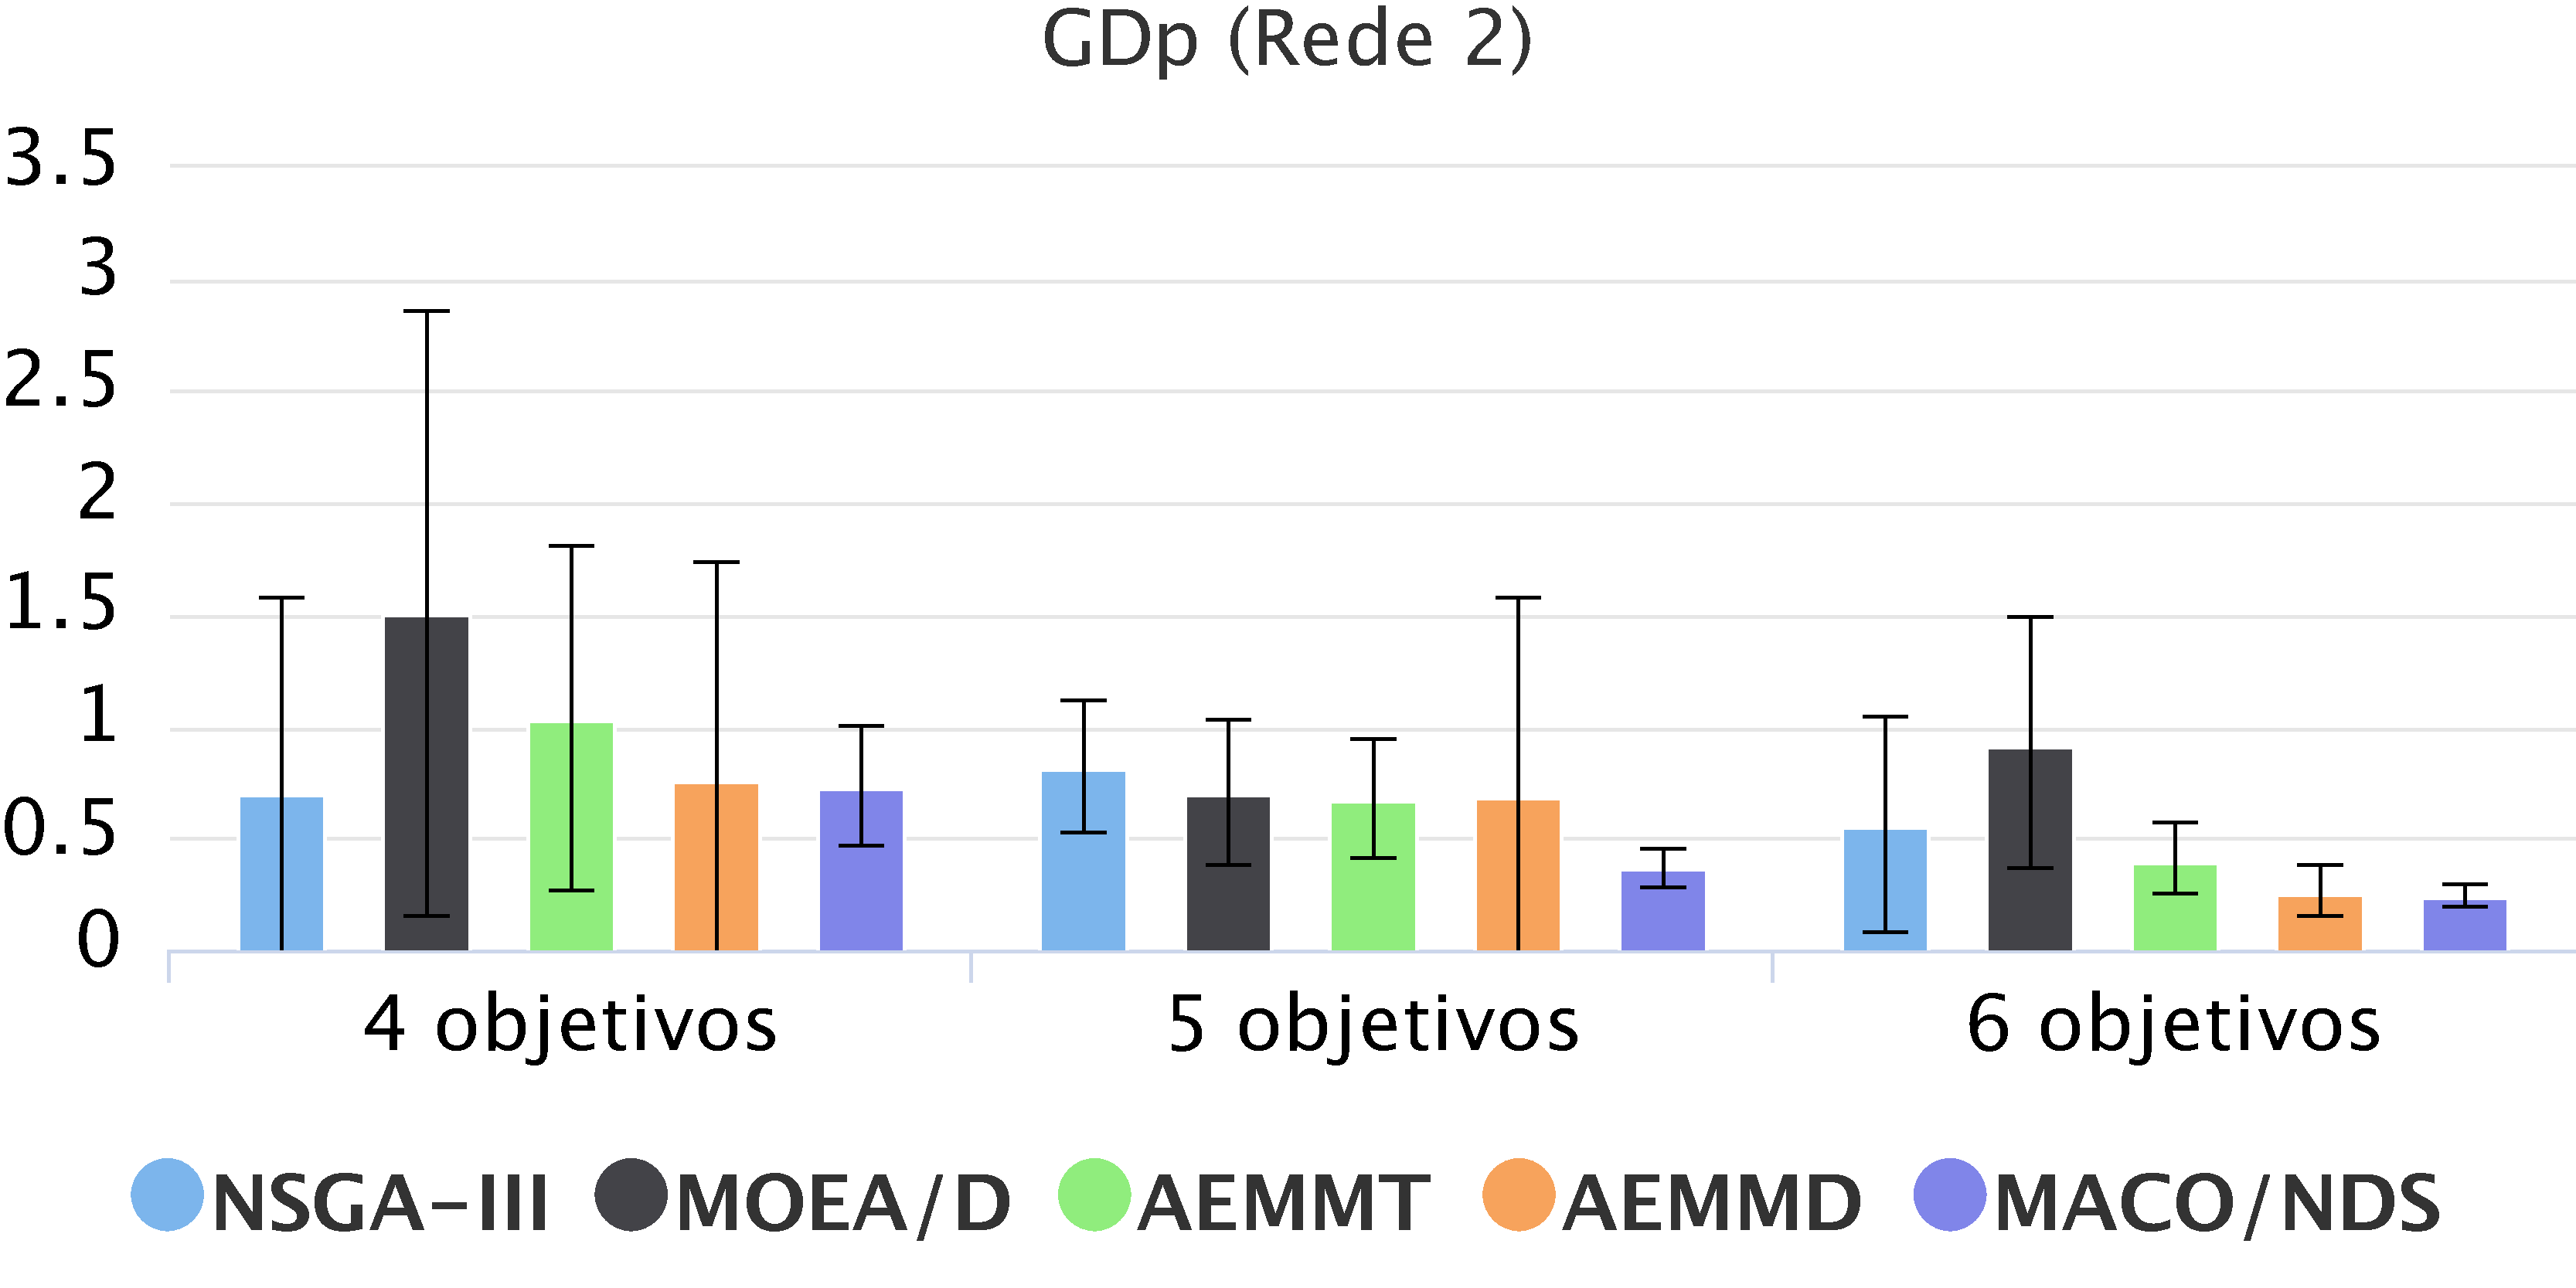
\includegraphics[width=0.5\textwidth]{cap_experimentos/figs/etapa3/gd-mrp-r2}
	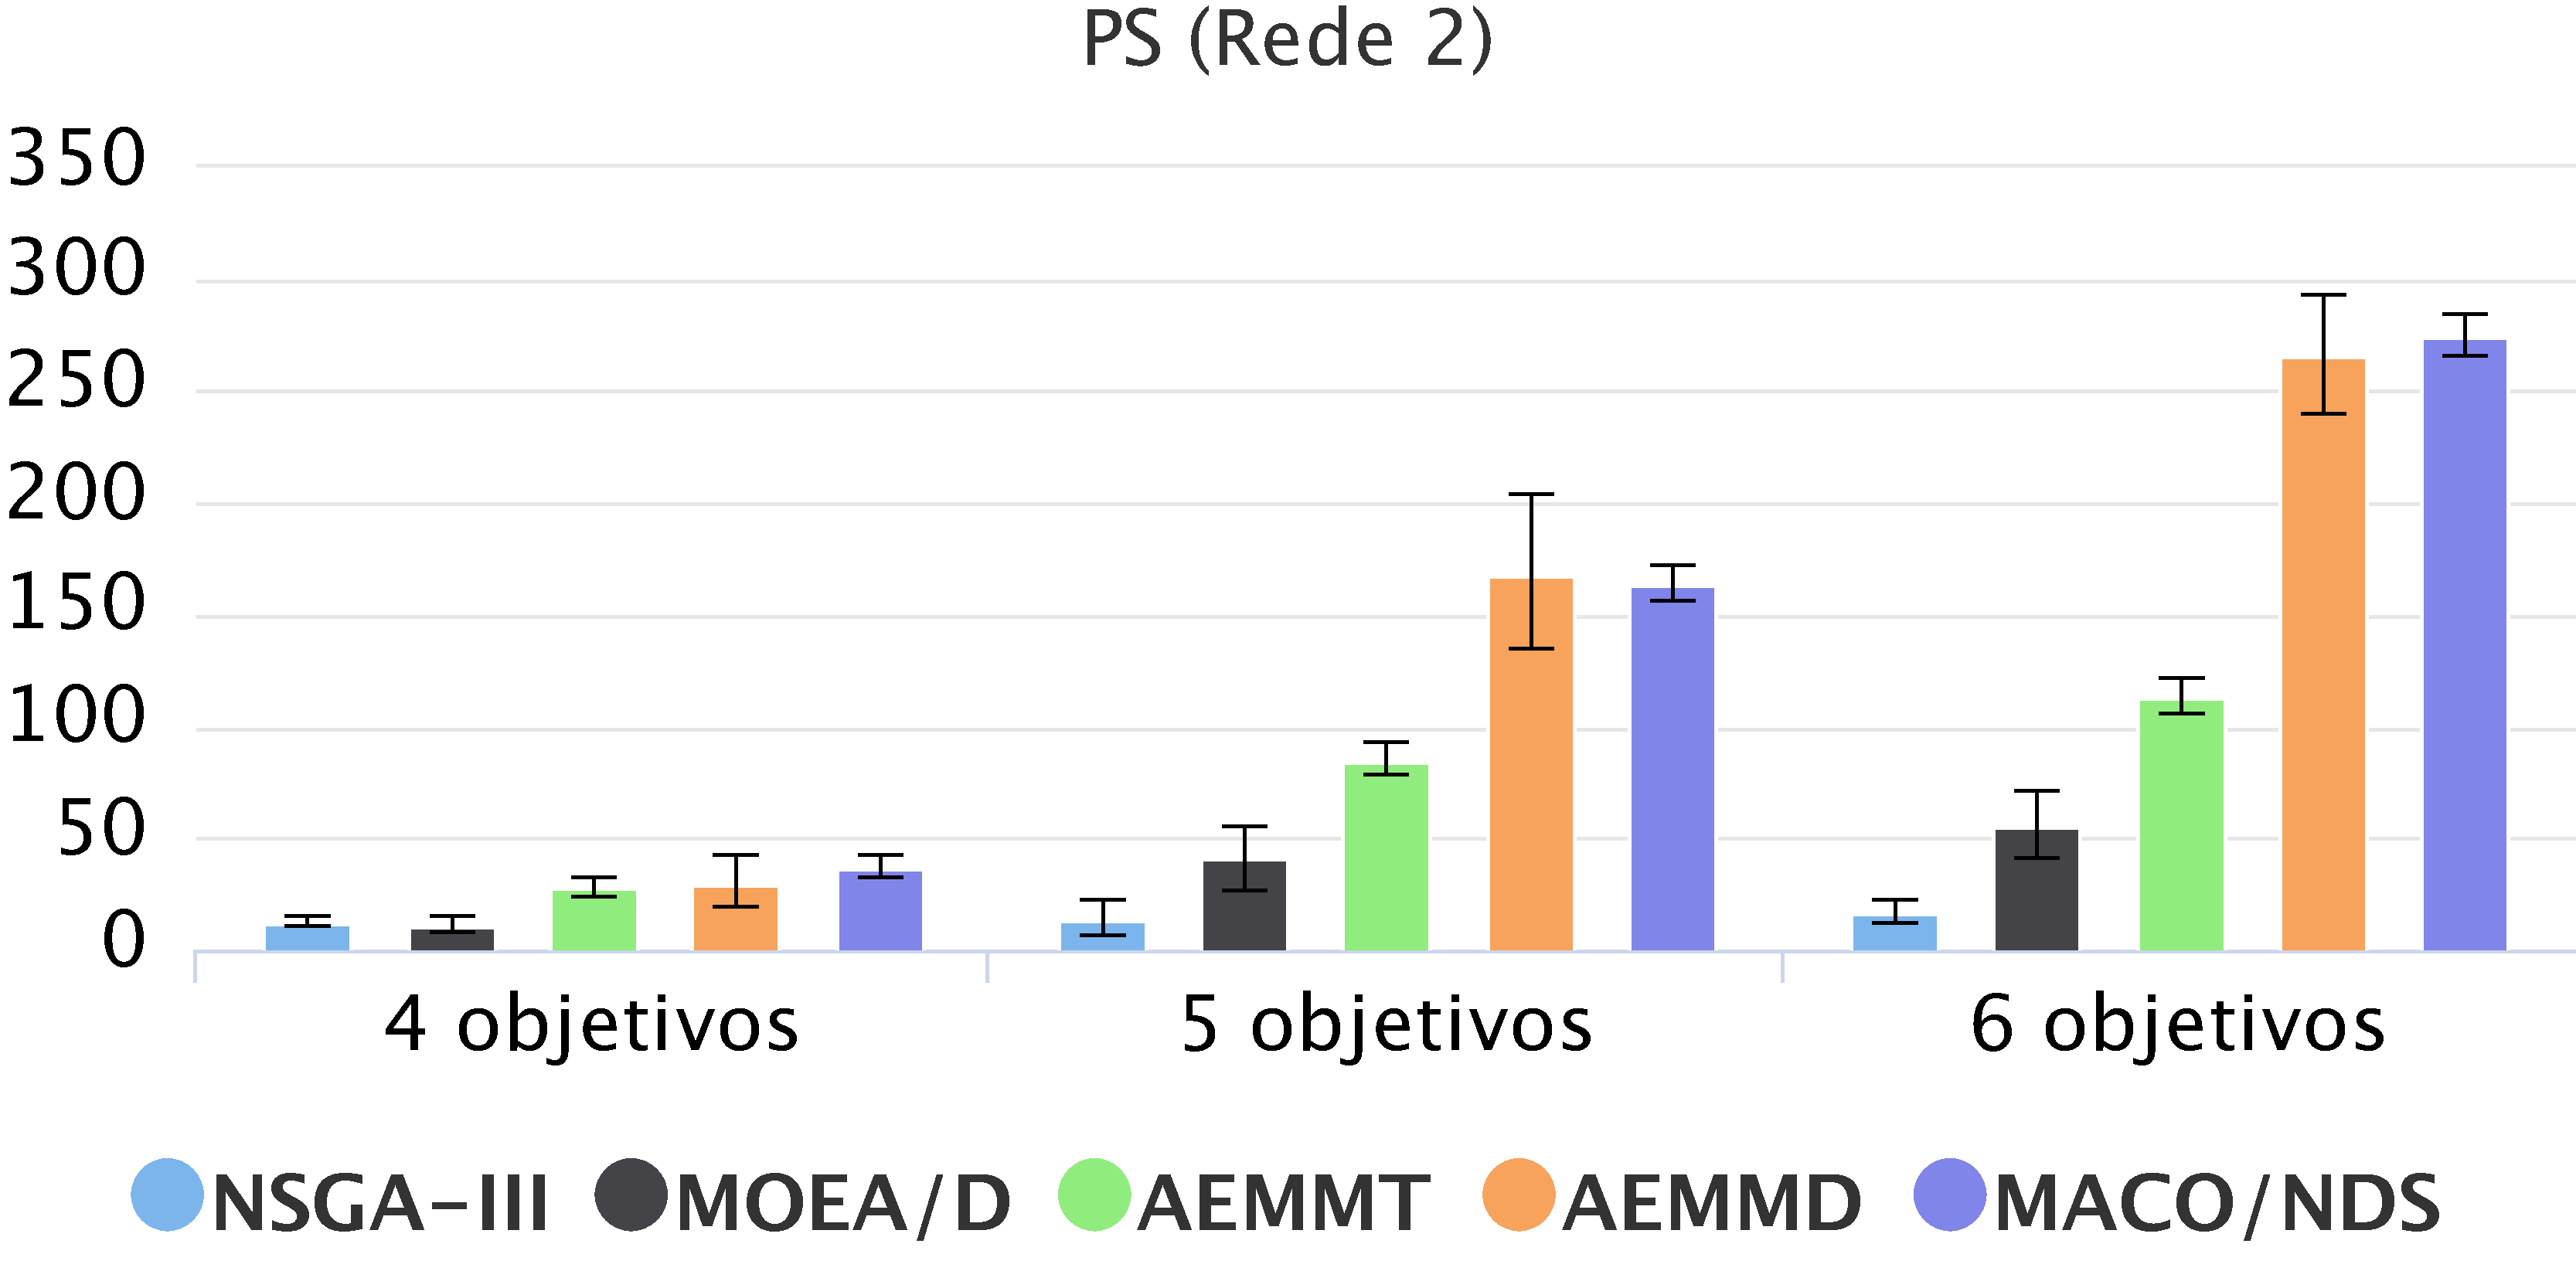
\includegraphics[width=0.5\textwidth]{cap_experimentos/figs/etapa3/ps-mrp-r2}
	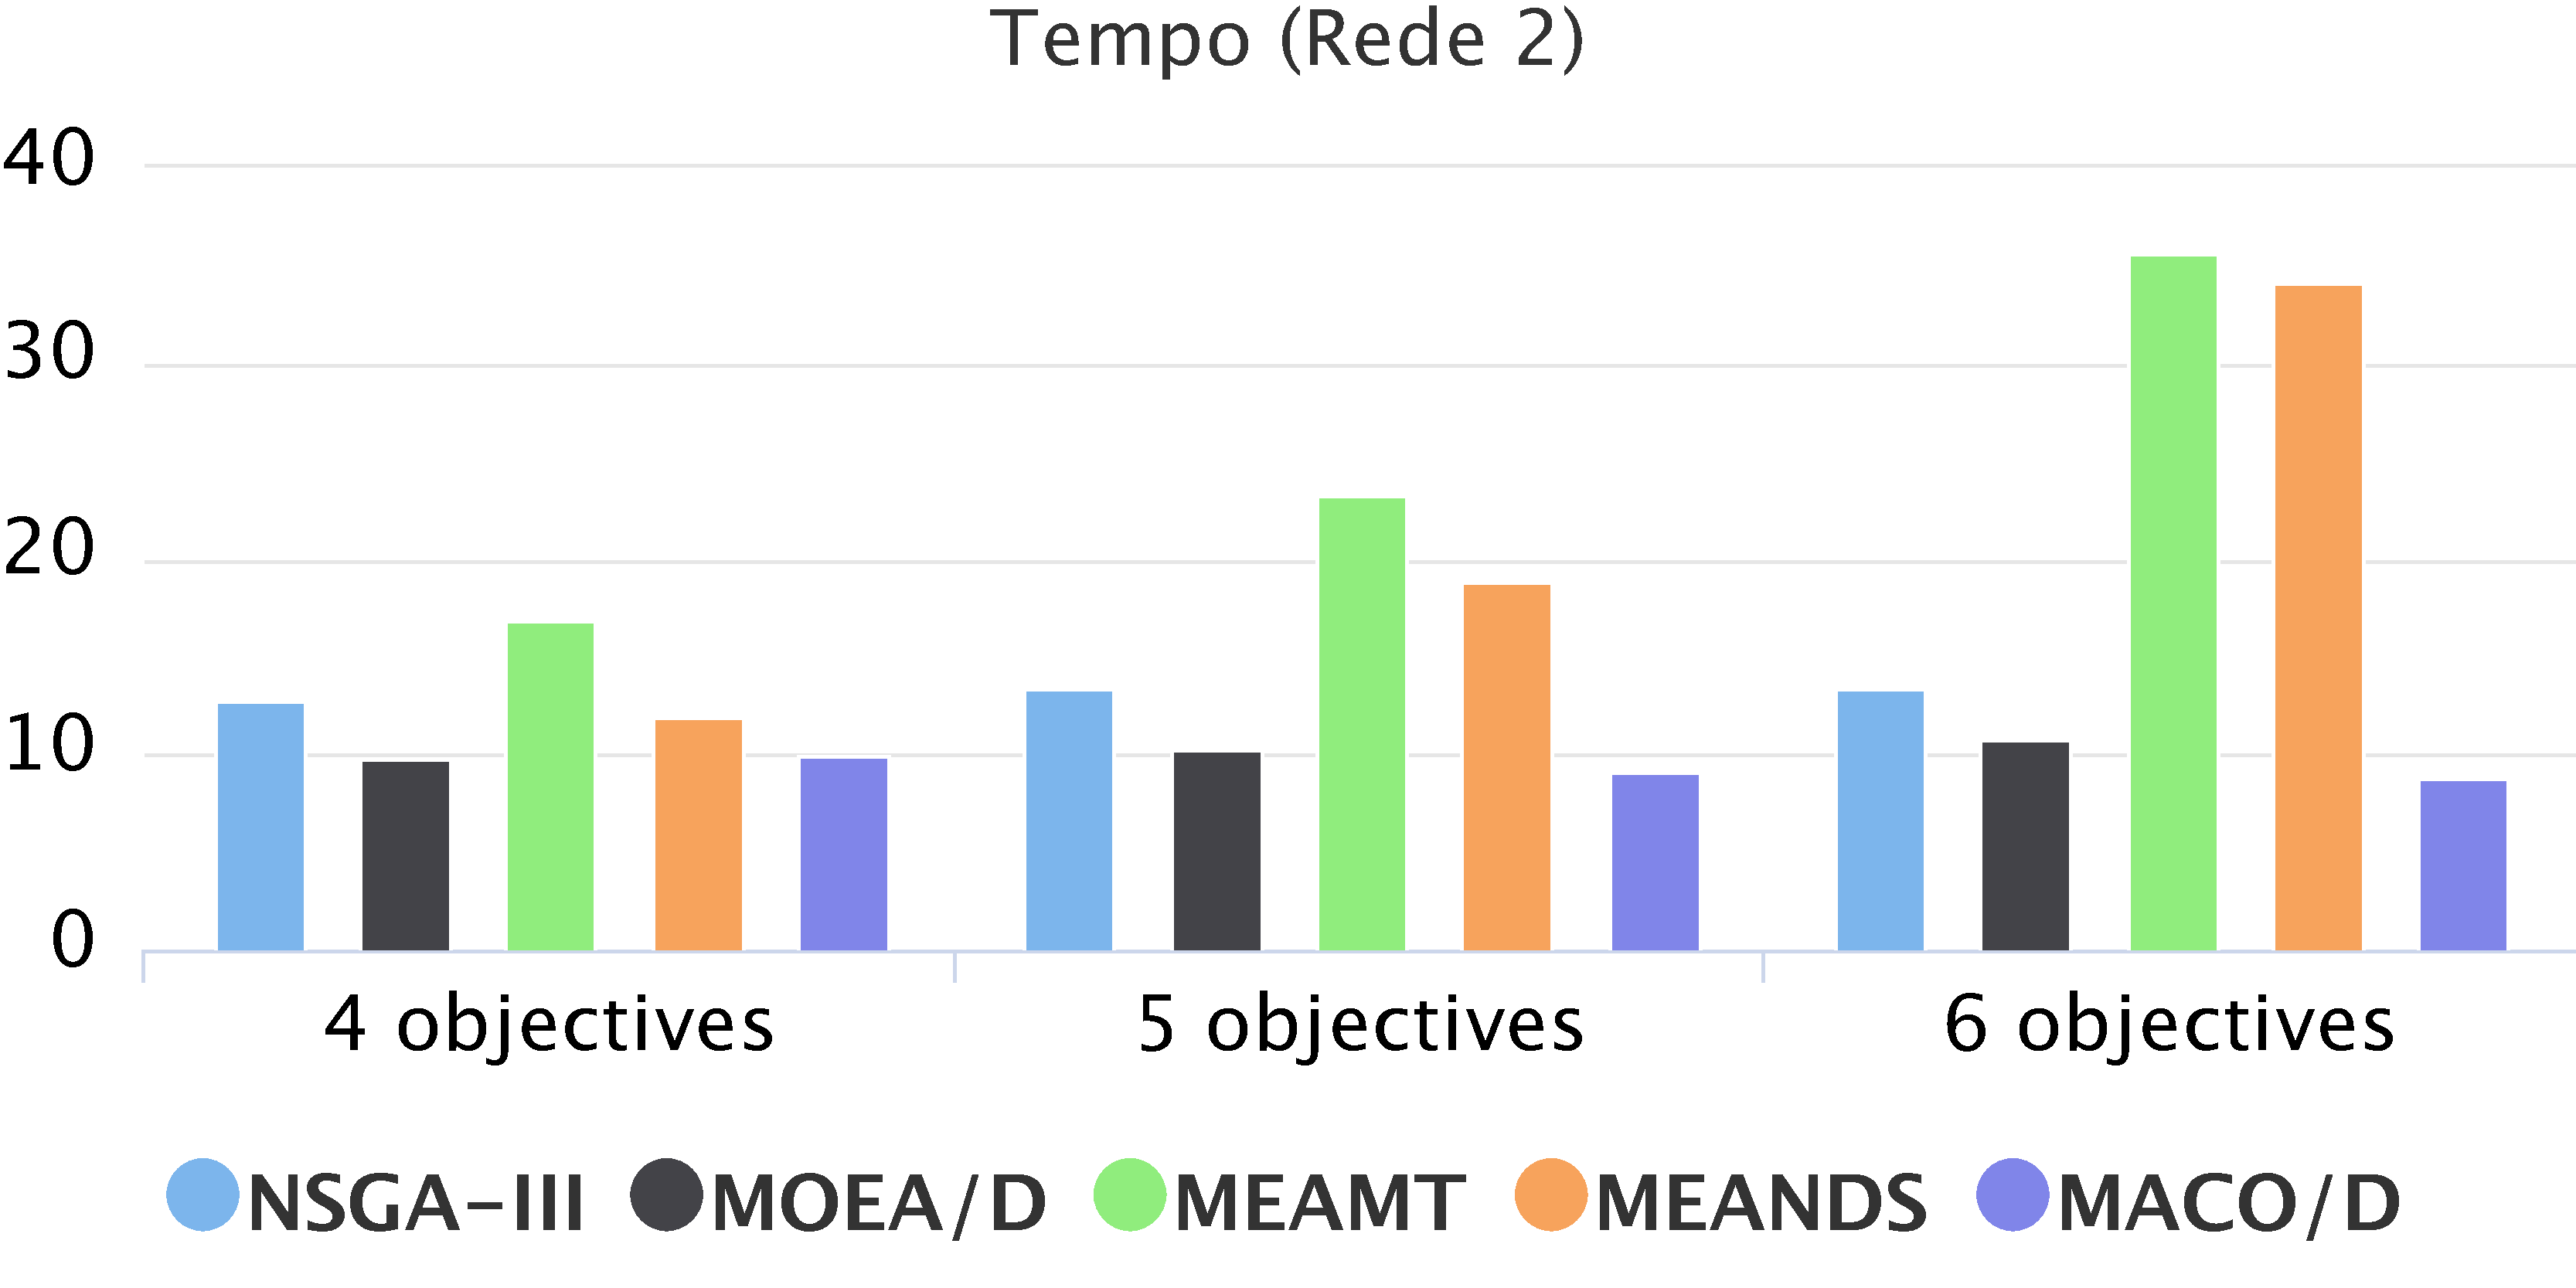
\includegraphics[width=0.5\textwidth]{cap_experimentos/figs/etapa3/time-mrp-r2}
	\caption{\label{fig_exp3_prm_r2}Desempenho dos algoritmos na 3ª etapa para o PRM na rede 2}
\end{figure*}

A \autoref{fig_exp3_prm_r2} apresenta os resultados obtidos pelos algoritmos para a rede 2. Apesar de mais complexa, os gráficos apresentam um comportamento similar ao da instância anterior (rede 1). O AEMMD obtém as menores taxas de erro, seguido pelo AEMMT. Dentre as soluções incorretas encontradas, o MACO/NDS é o algoritmo que alcança os menores valores para a métrica $GD$, sendo seguido de perto pelo AEMMT e pelo AEMMD. Considerando a métrica $PS$, os melhores valores foram encontrados pelo AEMMD, mas com uma diferença muito pequena em relação ao MACO/NDS. Os piores valores de $PS$ são retornados pelo NSGA-III. Tal comportamento é decorrência da limitação do algoritmo quanto ao crescimento do Pareto. Analisando o tempo médio de execução, o método mais rápido é o MOEA/D e o mais lento é o AEMMT.

\begin{figure*}[!htbp]
	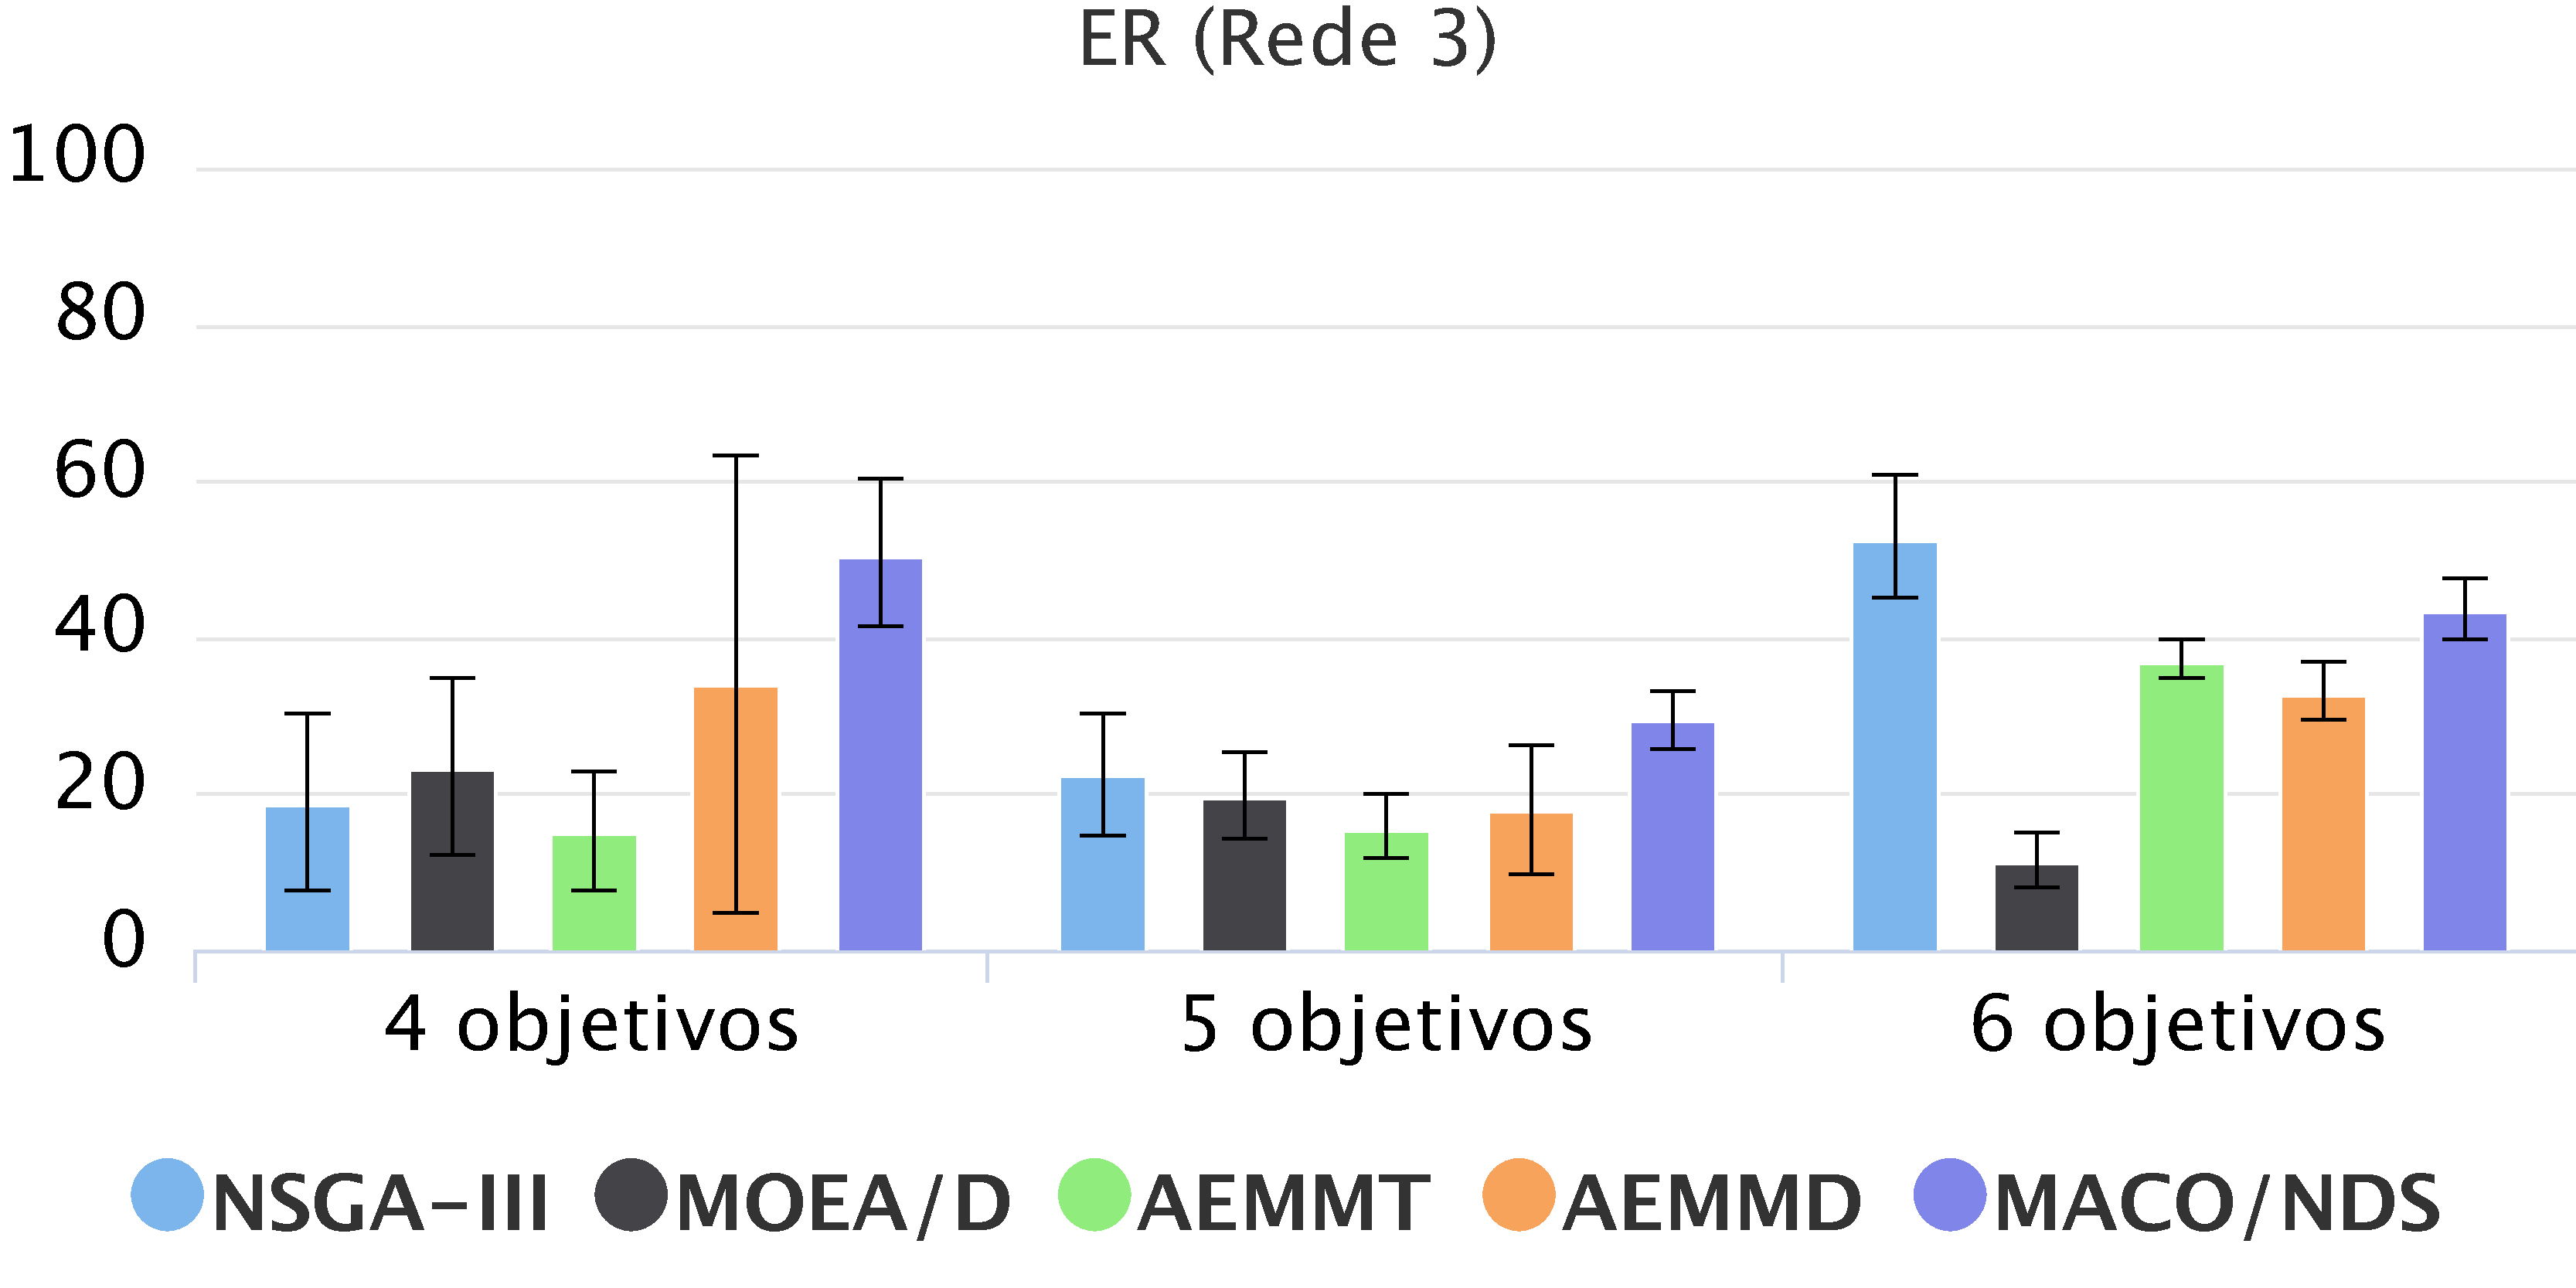
\includegraphics[width=0.5\textwidth]{cap_experimentos/figs/etapa3/er-mrp-r3}
	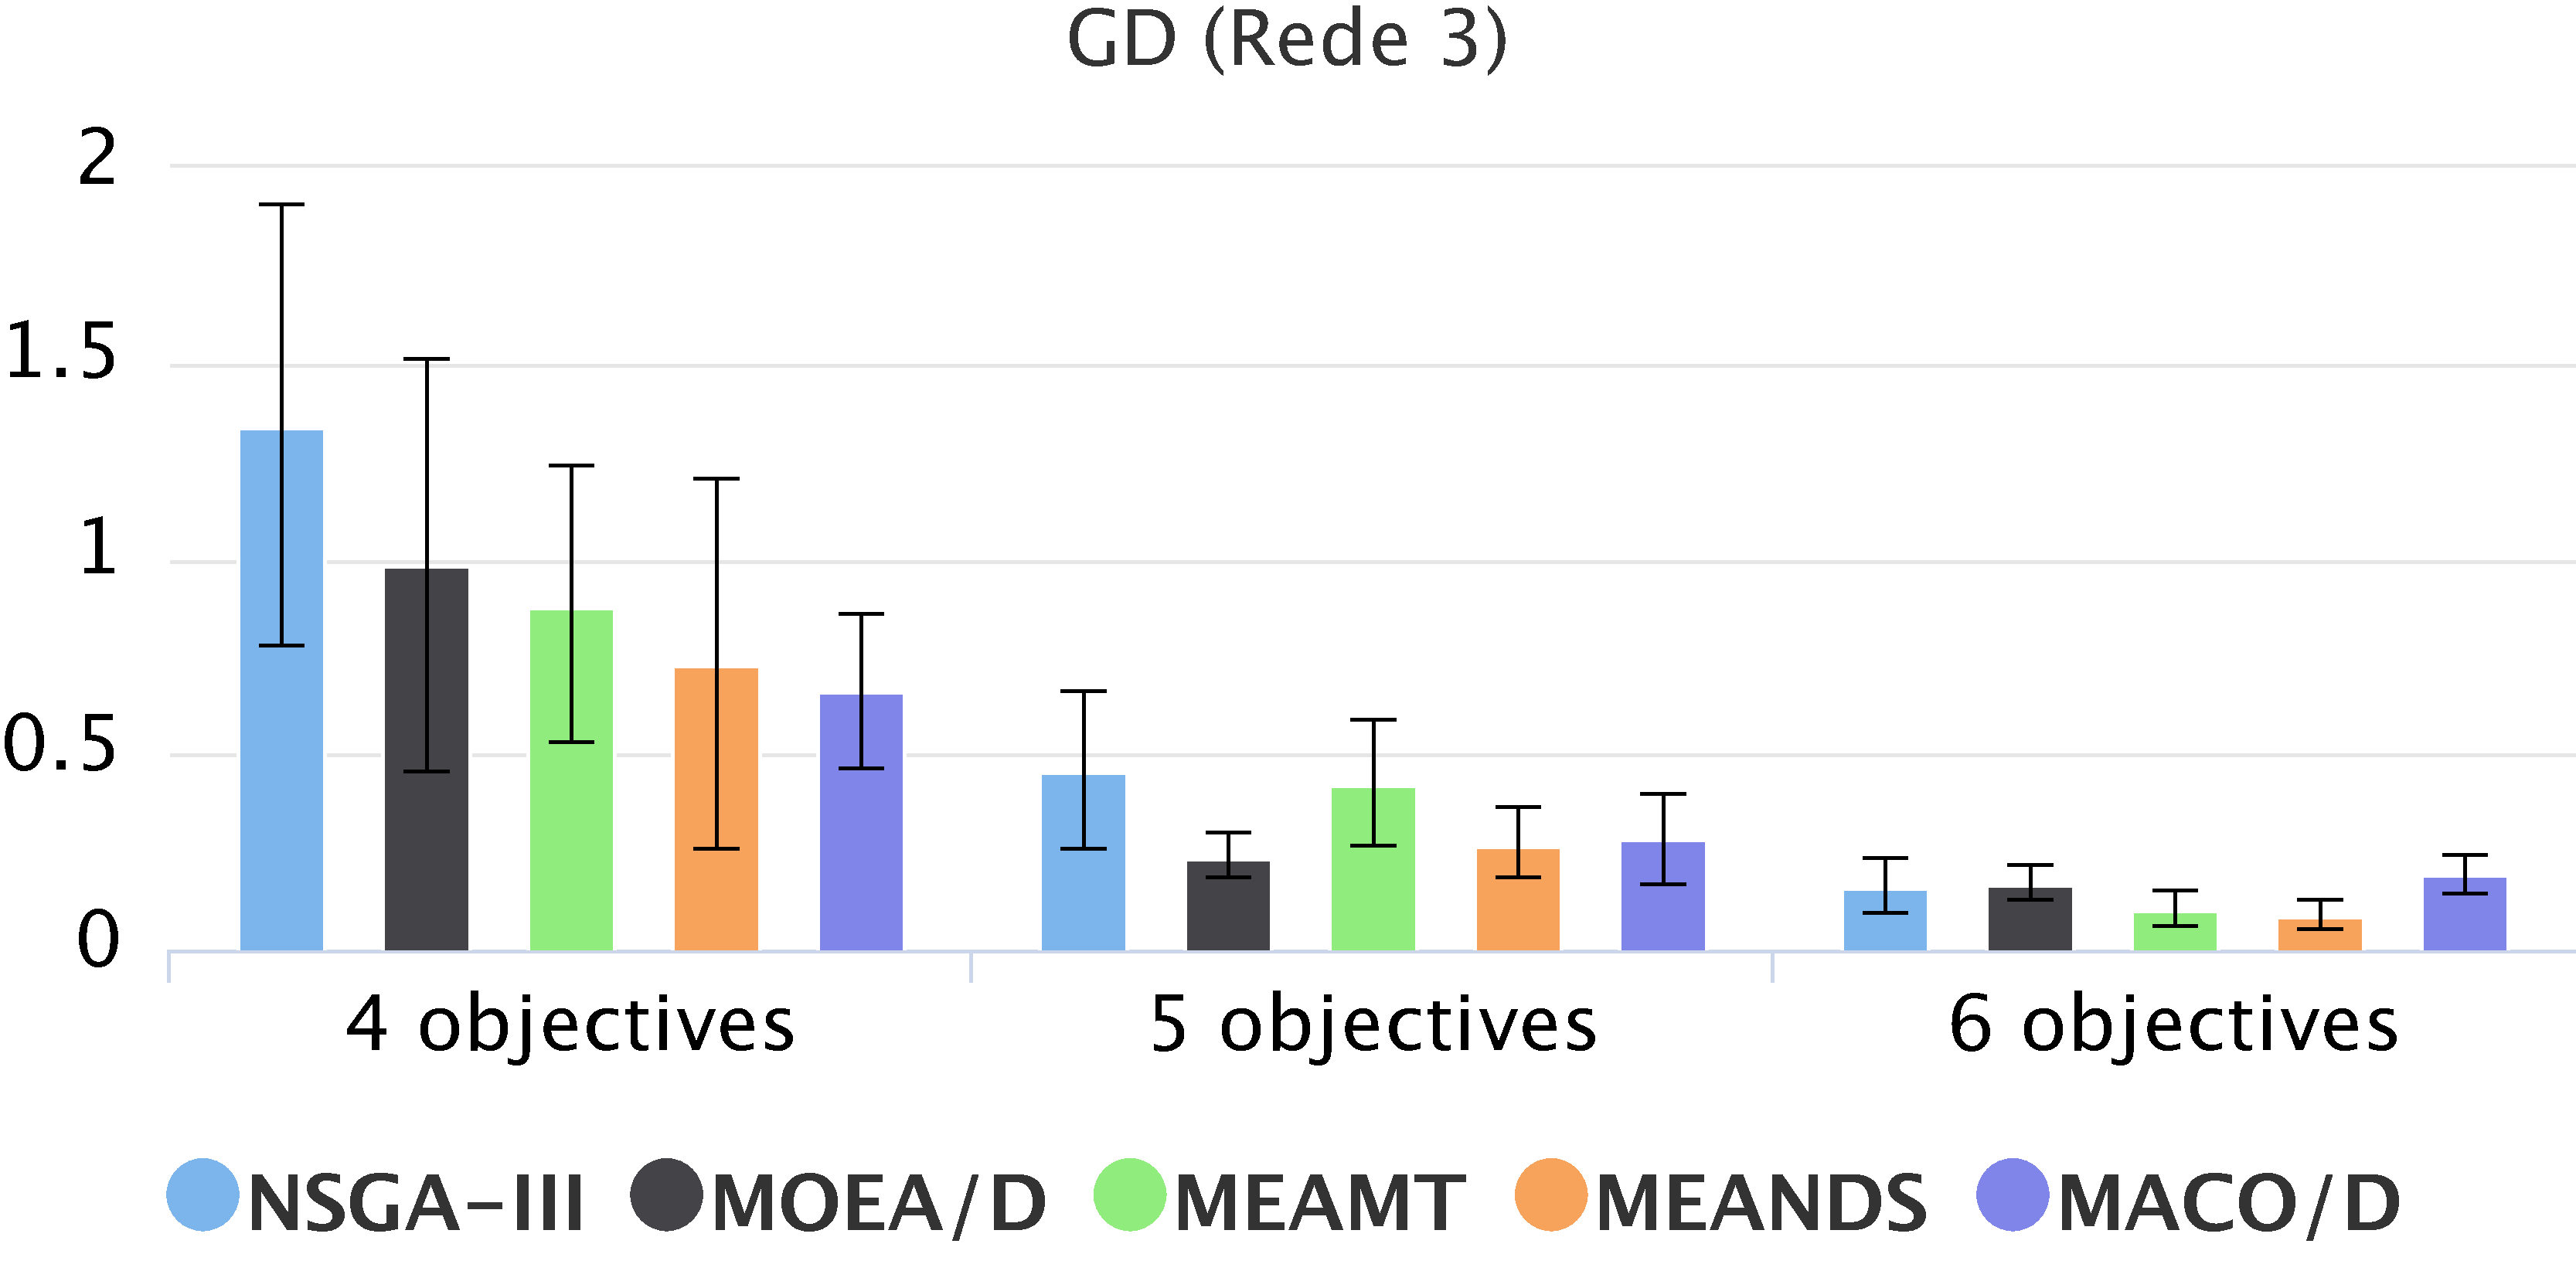
\includegraphics[width=0.5\textwidth]{cap_experimentos/figs/etapa3/gd-mrp-r3}
	\includegraphics[width=0.5\textwidth]{cap_experimentos/figs/etapa3/ps-mrp-r3}
	\includegraphics[width=0.5\textwidth]{cap_experimentos/figs/etapa3/time-mrp-r3}
	\caption{\label{fig_exp3_prm_r3}Desempenho dos algoritmos na 3ª etapa para o PRM na rede 3}
\end{figure*}

A \autoref{fig_exp3_prm_r3} apresenta o desempenho dos algoritmos no PRM considerando a rede 3, o AEMMT encontra as melhores taxas de erro para 4 e 5 objetivos, enquanto que o MOEA/D consegue o melhor resultado para 6 objetivos. O NSGA-III produz o segundo menor $ER$ no problema de 4 objetivos, mas é o segundo pior para 5 objetivos e o pior com 6 objetivos. O menor $GD$ no problema com 4 objetivos é dado pelo MACO/NDS, enquanto o AEMMT obtém os melhores valores nos problemas com 5 e 6 objetivos. As maiores fronteiras de Pareto são encontradas pelo AEMMD e MACO/NDS, sendo o AEMMD o melhor entre os dois. O algoritmo mais rápido é o MACO/NDS, executando em tempo 5 vezes menor que o método mais lento (AEMMT).

\begin{figure*}[!htbp]	
	\includegraphics[width=0.5\textwidth]{cap_experimentos/figs/etapa3/er-mrp-todos}
	\includegraphics[width=0.5\textwidth]{cap_experimentos/figs/etapa3/gd-mrp-todos}
	\includegraphics[width=0.5\textwidth]{cap_experimentos/figs/etapa3/ps-mrp-todos}
	\includegraphics[width=0.5\textwidth]{cap_experimentos/figs/etapa3/time-mrp-todos}
	\caption{\label{fig_exp3_prm_todos}Resultado consolidado da 3ª etapa considerando o PRM nas redes 1, 2 e 3}
\end{figure*}

Para analisar de forma conjunta os resultados das três redes, todos os experimentos são consolidados através da média aritmética das métricas de desempenho avaliadas. Esses resultados consolidados são apresentados na \autoref{fig_exp3_prm_todos}. De maneira geral, o NSGA-III consegue soluções de qualidade razoável, mas apresenta baixo $PS$ e um tempo médio de execução mediano. O MOEA/D obtém as melhores taxas de erro no problema de seis objetivos, mas tem um desempenho modesto nos problemas de 4 e 5 objetivos. O algoritmo também está entre os piores para as métricas $GD$ e $PS$. A velocidade de execução do MOEA/D é tão boa quanto a do MACO/NDS, sendo os dois algoritmos mais rápidos. Assim, o uso desse algoritmo pode ser uma opção quando o objetivo da busca é conseguir uma baixa taxa de erro em um curto tempo de execução, sem se preocupar com o $PS$. Analisando todas as métricas, os melhores resultados foram obtidos pelo AEMMD e nosso algoritmo (MACO/NDS). Com relação ao erro, o AEMMD consegue as melhores taxas, enquanto o MACO/NDS, juntamente com o NSGA-III, apresentam os piores valores. Analisando o $GD$, existe uma pouca diferença entre os algoritmos, mas o MACO/NDS gera melhores soluções que o AEMMD. Além disso, o desvio padrão do MACO/NDS é significativamente menor, tornando-o um método mais estável quanto à qualidade das soluções. Um desempenho similar também é observado para a métrica PS. Entretanto, nesse caso, o AEMMD produz as maiores fronteiras de Pareto que o MACO/NDS. Por outro lado, ao analisar o tempo médio de execução, observa-se que o MACO/NDS é consideravelmente mais rápido, chegando a executar em quase 5 vezes menos tempo. Considerando que o PRM é um problema sensível ao tempo de execução, apesar do AEMMD obter um desempenho razoavelmente superior nas métricas $ER$ e $PS$, o MACO/NDS é a melhor opção entre os algoritmos testados, pelo menos nos cenários analisados.

A principal diferença no desempenho do algoritmo proposto (MACO/NDS) em relação aos dois problemas investigados é o tempo de execução. Considerando os resultados do PMM apresentados na \autoref{fig_exp3_pmm_todos}, o MACO/NDS é o segundo algoritmo mais lento e seu tempo de execução está altamente relacionado ao número de objetivos. Na \autoref{fig_exp3_prm_todos}, que representa o comportamento geral dos algoritmos no PRM, observa-se o oposto, ou seja, o MACO/NDS é o algoritmo mais rápido e seu tempo de execução se mantém estável, independentemente da formulação de objetivos. Essa diferença de comportamento é decorrência do tamanho da fronteira de Pareto (soluções não dominadas). O processo de maior custo computacional no MACO/NDS é a atualização dos feromônios, onde é necessário recalcular o conjunto de soluções não-dominadas $nd$. A cada iteração, para toda solução criada, é necessário passar por todos elementos em $nd$ verificando a relação de não-dominância. Naturalmente, quanto maior o conjunto $nd$, mais caro se torna o processo. No PRM, foram encontradas fronteiras de Pareto de tamanho razoavelmente pequenos, todas com menos de 350 elementos. Nesse caso, para cada solução criada, é preciso fazer no máximo 350 comparações. No PMM, as fronteiras de Pareto são muito grandes. Por exemplo, no problema com 6 objetivos e 50 itens, a cardinalidade do conjunto $nd$ chega a ser maior que 4500 soluções. Quanto maior a quantidade de objetivos do problema, maior o número de soluções no Pareto e mais lento será a classificação de soluções não dominadas. Se o conjunto $nd$ é pequeno até mesmo para a maior quantidade de objetivos (caso do PRM), o processo será rápido e o tempo de execução não será muito diferente entre as formulações de objetivos. Por outro lado, se a cardinalidade de $nd$ é muito grande e cresce muito com o aumento da quantidade de objetivos, o tempo necessário para se atualizar os feromônios será muito alto e terá grande variação conforme a formulação de objetivos.

A fim de melhor comparar o MACO/NDS aos algoritmos AEMMT e AEMMD, realizou-se o teste de hipótese teste Z (\textit{Z-test}) com 5\% de significância ($\alpha=0,05$). Os resultados são mostrados nas Tabelas \ref{tab_ztest_meamt} e \ref{tab_ztest_meams}. Em ambas as tabelas, uma célula de fundo verde representa um cenário onde o MACO/NDS obteve melhor resultado que seu adversário, vermelho significa que o adversário foi melhor e a célula branca indica empate.

\begin{table}[htb]
	\centering
	\def\arraystretch{1.0}
	\caption{Testes de hipótese entre o MACO/NDS e o AEMMT para os problemas investigados}
	\label{tab_ztest_meamt}
	\begin{tabular}{llllllllll}
		& \multicolumn{3}{l}{\textbf{4 objectives}} & \multicolumn{3}{l}{\textbf{5 objectives}} & \multicolumn{3}{l}{\textbf{6 objectives
		}} \\
		\textbf{Instance} & \textbf{ER} & \textbf{GD} & \textbf{PS} & \textbf{ER} & \textbf{GD} & \textbf{PS} & \textbf{ER} & \textbf{GD} & \textbf{PS} \\ \hline
		30 items & \cellcolor{white} $=$ & \cellcolor{table-green} $<$ & \cellcolor{table-green} $>$ & \cellcolor{table-red} $>$ & \cellcolor{table-green} $<$ & \cellcolor{table-green} $>$ & \cellcolor{table-red} $>$ & \cellcolor{table-green} $<$ & \cellcolor{table-green} $>$ \\
		40 items & \cellcolor{table-green} $<$ & \cellcolor{table-green} $<$ & \cellcolor{table-green} $>$ & \cellcolor{table-green} $<$ & \cellcolor{table-green} $<$ & \cellcolor{table-green} $>$ & \cellcolor{table-red} $>$ & \cellcolor{table-green} $<$ & \cellcolor{table-green} $>$ \\
		50 items & \cellcolor{table-green} $<$ & \cellcolor{white} $=$ & \cellcolor{table-green} $>$ & \cellcolor{table-green} $<$ & \cellcolor{table-green} $<$ & \cellcolor{table-green} $>$ & \cellcolor{table-red} $>$ & \cellcolor{table-green} $<$ & \cellcolor{table-green} $>$ \\  \hline 
		Rede 1 & \cellcolor{table-red} $>$ & \cellcolor{table-green} $<$ & \cellcolor{table-red} $<$ & \cellcolor{table-red} $>$ & \cellcolor{table-green} $<$ & \cellcolor{table-green} $>$ & \cellcolor{table-red} $>$ & \cellcolor{table-green} $<$ & \cellcolor{table-green} $>$ \\
		Rede 2 & \cellcolor{table-red} $>$ & \cellcolor{table-green} $<$ & \cellcolor{table-green} $>$ & \cellcolor{table-red} $>$ & \cellcolor{table-green} $<$ & \cellcolor{table-green} $>$ & \cellcolor{table-green} $<$ & \cellcolor{table-green} $<$ & \cellcolor{table-green} $>$ \\
		Rede 3 & \cellcolor{table-red} $>$ & \cellcolor{table-green} $<$ & \cellcolor{table-red} $<$ & \cellcolor{table-red} $>$ & \cellcolor{table-green} $<$ & \cellcolor{table-green} $>$ & \cellcolor{table-red} $>$ & \cellcolor{table-red} $>$ & \cellcolor{table-green} $>$ \\  \hline 
	\end{tabular}
\end{table}

\begin{table}[htb]
	\centering
	\def\arraystretch{1.0}
	\caption{Testes de hipótese entre o MACO/NDS e o AEMMD para os problemas investigados}
	\label{tab_ztest_meams}
	\begin{tabular}{llllllllll}
		& \multicolumn{3}{l}{\textbf{4 objectives}} & \multicolumn{3}{l}{\textbf{5 objectives}} & \multicolumn{3}{l}{\textbf{6 objectives
		}} \\
		\textbf{Instance} & \textbf{ER} & \textbf{GD} & \textbf{PS} & \textbf{ER} & \textbf{GD} & \textbf{PS} & \textbf{ER} & \textbf{GD} & \textbf{PS} \\ \hline
		30 items & \cellcolor{table-green} $<$ & \cellcolor{table-green} $<$ & \cellcolor{table-green} $>$ & \cellcolor{table-green} $<$ & \cellcolor{table-red} $>$ & \cellcolor{table-green} $>$ & \cellcolor{table-green} $<$ & \cellcolor{table-red} $>$ & \cellcolor{table-green} $>$ \\
		40 items & \cellcolor{table-green} $<$ & \cellcolor{table-red} $>$ & \cellcolor{table-green} $>$ & \cellcolor{table-green} $<$ & \cellcolor{table-red} $>$ & \cellcolor{table-green} $>$ & \cellcolor{table-green} $<$ & \cellcolor{table-red} $>$ & \cellcolor{table-green} $>$ \\
		50 items & \cellcolor{table-green} $<$ & \cellcolor{table-green} $<$ & \cellcolor{table-green} $>$ & \cellcolor{table-green} $<$ & \cellcolor{table-green} $<$ & \cellcolor{table-green} $>$ & \cellcolor{table-green} $<$ & \cellcolor{table-green} $<$ & \cellcolor{table-green} $>$ \\  \hline 
		Rede 1 & \cellcolor{table-red} $>$ & \cellcolor{table-green} $<$ & \cellcolor{table-red} $<$ & \cellcolor{table-red} $>$ & \cellcolor{table-green} $<$ & \cellcolor{table-red} $<$ & \cellcolor{table-red} $>$ & \cellcolor{table-green} $<$ & \cellcolor{table-red} $<$ \\
		Rede 2 & \cellcolor{table-red} $>$ & \cellcolor{white} $=$ & \cellcolor{table-green} $>$ & \cellcolor{table-red} $>$ & \cellcolor{table-green} $<$ & \cellcolor{table-red} $<$ & \cellcolor{table-red} $>$ & \cellcolor{table-green} $<$ & \cellcolor{table-green} $>$ \\
		Rede 3 & \cellcolor{table-red} $>$ & \cellcolor{table-green} $<$ & \cellcolor{table-red} $<$ & \cellcolor{table-red} $>$ & \cellcolor{white} $=$ & \cellcolor{table-red} $<$ & \cellcolor{table-red} $>$ & \cellcolor{table-red} $>$ & \cellcolor{table-red} $<$ \\  \hline 
	\end{tabular}
\end{table}

No PMM, se o tempo de execução é uma preocupação, a melhor alternativa é o algoritmo MOEA/D, que executa em tempo recorde e produz bons resultados. Se a rapidez do algoritmo não é tão importante e deseja-se encontrar um conjunto de soluções mais próximo do Pareto real, o MACO/NDS é o algoritmo mais indicado. No PRM, o método que representa melhor relação entre qualidade e tempo é o MACO/NDS. Por outro lado, se tempo não é importante, o AEMMD pode ser preferível.

A partir desses experimentos, foi elaborado um artigo científico que será publicado no 2018 \textit{IEEE Congress on Evolutionary Computation} \cite{Franca2018}.

\section{Etapa 4: Análise com hipervolume}
\label{section_experimentos_etapa4}

Na quarta etapa, os experimentos visam avaliar os algoritmos de otimização many-objective NSGA-III, MOEA/D, AEMMT, AEMMD e MACO/NDS em instâncias complexas do PMM e PRM utilizando a métrica hipervolume, a qual independe da estimação e/ou do conhecimento prévio da fronteira de Pareto. Esses experimentos são necessários, pois as etapas anteriores testaram apenas problemas com complexidade razoável, onde é possível estimar previamente a Fronteira de Pareto. Em grande parte dos problemas reais, esse conhecimento prévio é impraticável. Por exemplo, com a inclusão de mais itens no PMM ou o uso de redes mais complexas no PRM torna inviável a obtenção da fronteira de Pareto e faz necessária a utilização de uma métrica não-paramétrica, neste caso o hipervolume, para avaliar o desempenho dos algoritmos. Nesses experimentos são utilizadas duas novas redes para o PRM e uma nova instância do PMM, com 200 itens.

A fim de testar propriamente o comportamento dos algoritmos em espaços de busca mais complexos que os utilizados nos experimentos das etapas 1 e 3, lançou-se mão de duas novas redes (redes 4 e 5) e duas novas instâncias do problema da mochila (100 e 200 itens). Como não é possível extrair Paretos estáveis para as redes $R_3$, $R_4$ e $R_5$, nem para os problemas da mochila com 50, 100 e 200 itens, não é interessante basear-se em métricas dependentes de tais Paretos para se tirar conclusões. Por isso, nesta etapa, testa-se unicamente as métrica hipervolume e tempo, independentes do Pareto.

O hipervolume, junto ao \textit{inverse generational distance} $(IDG)$, são as métricas mais utilizadas na literatura para se avaliar algoritmos many-objectives. O hipervolume, como explicado no início deste capítulo, calcula o volume da figura geométrica formada pelas distâncias das soluções a um ponto de referência pré-definido. Os pontos de referência utilizados em cada cenário são apresentados na tabela \ref{table_exp4_pts_referencia}.

Neste conjunto de experimentos, assim como na etapa 3, comparou-se apenas os cenários many-objectives, com 4, 5 e 6 objetivos. Por esse motivo, ficaram de fora dos testes os algoritmos clássicos NSGA-II e SPEA2. Em contra-partida incluiu-se 3 novos métodos many-objectives na comparação: SPEA2-SDE (AG), MOACS (ACO) e MOEA/D-ACO (ACO). Os parâmetros utilizados para cada método podem ser encontrados na tabela \ref{table_exp4_params}.

\begin{table}[!htbp]
	\caption{Parâmetros utilizados para o PRM e o PMM na etapa 4 de experimentos.}
	\label{table_exp4_params}
	\begin{center}
		\begin{tabular}{c|r|r}
			\textbf{Parâmetro} & \textbf{PRM} &  \textbf{PMM} \\ %\hline
			\hline
			Tamanho da população               &    90 &      150 \\ %\hline
			Número de comparações        &   9000 &      15000 \\ %\hline
			Taxa de crossover                & 100\% &    100\% \\ %\hline
			Taxa de mutação                 &  20\% &      5\% \\ %\hline
			Tamanho da vizinhança (MOEA/D e MOEA/D-ACO)    &    10 &       10 \\ %\hline
			Tamanho das tabelas (MEAMT)   &    30 &       50 \\ %\hline
			Tamanho da tabela de dominância (MEAMT) &    90 &      150 \\ %\hline
			Número de divisões (NSGA-III)&     8 &        8 \\ %\hline
			$\alpha, \beta, \rho$ (ACO's)& 1, 2, 0.3 & 1, 4.3, 0.3 \\ %\hline
			Intervalo de valores para os feromônios (ACO's)& [0.1, 0.9] & [0.1, 0.9] \\ %\hline
			$\delta$ (MOEA/D-ACO)& 0.2 & 0.2 \\ %\hline
			Número de formigas e grupos (MOEA/D-ACO)*& 6 & variável \\ %\hline
			Número de grupos de formigas (MOEA/D-ACO)*& 3 & 3 \\ %\hline
			Taxa de elitismo (MOEA/D-ACO)& 0.9 & 0 \\ %\hline
			Tamanho das amostras (MACO/NDS)& 10 & 10 \\  %\hline
			Tamanho do grupo de estruturas ativas (MACO/NDS)& 5 & 5 \\
			\hline
		\end{tabular}
	\end{center}
\end{table}

Sobre os parâmetros marcados com ``*'' na tabela \ref{table_exp4_params}, a quantidade de formigas depende do parâmetro $H$, do artigo original do algoritmo \cite{Ke2013}, enquanto o tamanho dos grupos depende de outro parâmetro, $K$, também descrito no mesmo artigo. Ambos os parâmetros $H$ e $K$ servem como guia para gerar os pesos aleatórios das formigas e dos grupos, quanto maior o valor de $H$, maior será o número de formigas, o mesmo vale para $K$ e a quantidade de grupos. De toda maneira, o número de iterações no laço principal é ajustado para que sempre se tenha o mesmo número de comparações (9000 no PRM e 15000 no PMM). Os valores de $H$ usados no PMM foram: $H=8$ para 4 objetivos, $H=6$ para 5 objetivos e $H=5$ para 6 objetivos.

Com relação aos algoritmos NSGA-III e SPEA2-SDE, na etapa 4, tomou-se uma outra atitude em relação às limitações no tamanho do Pareto. Ao invés de impedir o conjunto de soluções não-dominadas de crescerem além do tamanho máximo da população, ajustou-se esse limite para coincidi-lo com o tamanho médio dos Paretos encontrados pelos algoritmos que retornaram os maiores conjuntos de soluções. Dessa forma, ambos NSGA-III e SPEA2-SDE podem encontrar Paretos tão grandes quanto os demais algoritmos. A tabela \ref{table_exp4_pts_referencia} mostra os limites utilizados para cada cenário de teste.

\begin{table}[!htbp]
	\centering
	\caption{Ponto de referência e limitações no tamanho do Pareto usados para cada cenário de teste}
	\label{table_exp4_pts_referencia}
	\begin{tabular}{clll}
		\textbf{Instância}                                                       & \textbf{Obj.} & \textbf{Ponto de referência}                          & \textbf{Limite} \\ \hline
		\multirow{3}{*}{\begin{tabular}[c]{@{}c@{}}PMM\\ 50 itens\end{tabular}}  & 4             & {[}-15665, -17464, -19122, -16978{]}                   & 600             \\
		& 5             & {[}-15948, -15980, -14696, -14800, -14610{]}           & 1400            \\
		& 6             & {[}-16094, -14354, -12511, -14240, -17865, -11801{]}   & 4500            \\ \hline
		\multirow{3}{*}{\begin{tabular}[c]{@{}c@{}}PMM\\ 100 itens\end{tabular}} & 4             & {[}-30442, -25071, -30870, -29800{]}                   & 1300            \\
		& 5             & {[}-30673, -30266, -30171, -30922, -28821{]}           & 3200            \\
		& 6             & {[}-29389, -27406, -30824, -32040, -30531, -30171{]}   & 3400            \\ \hline
		\multirow{3}{*}{\begin{tabular}[c]{@{}c@{}}PMM\\ 200 itens\end{tabular}} & 4             & {[}-64608, -58090, -61540, -59399{]}                   & 1500            \\
		& 5             & {[}-62513, -63014, -58939, -64477, -65814{]}           & 3000            \\
		& 6             & {[}-59835, -60434, -65232, -60525, -60843, -60753{]}   & 3200            \\ \hline
		\multirow{3}{*}{\begin{tabular}[c]{@{}c@{}}PRM\\ Rede 3\end{tabular}}    & $P_4$         & {[}0.758449304, 283, 115, 52{]}                       & 90              \\
		& $P_5$         & {[}0.47215566, 0.776046738, 304, 159, 56{]}           & 250             \\
		& $P_6$         & {[}0.471416081, 0.776046738, 310, 159, 56, 83.459{]}  & 400             \\ \hline
		\multirow{3}{*}{\begin{tabular}[c]{@{}c@{}}PRM\\ Rede 4\end{tabular}}    & $P_4$         & {[}0.717830882, 185, 107, 33{]}                       & 90              \\
		& $P_5$         & {[}0.454221232, 0.776046738, 256, 157, 42{]}          & 200             \\
		& $P_6$         & {[}0.457194502, 0.776046738, 239, 157, 40, 80.667{]}  & 350             \\ \hline
		\multirow{3}{*}{\begin{tabular}[c]{@{}c@{}}PRM\\ Rede 5\end{tabular}}    & $P_4$         & {[}0.776046738, 259, 146, 43{]}                       & 90              \\
		& $P_5$         & {[}0.458729196, 0.776046738, 296, 166, 49{]}          & 100             \\
		& $P_6$         & {[}0.458729196, 0.776046738, 287, 177, 48, 101.938{]} & 250             \\ \hline
	\end{tabular}
\end{table}

Na tabela \ref{table_exp4_pts_referencia}, os valores para o PMM são negativos, pois todos os algoritmos foram implementados para lidar com problemas de minimização. Dessa forma, como no problema da mochila deseja-se maximizar o valor de lucro carregado na mochila, todos os valores são multiplicados por -1 antes de se iniciar a busca.

Com relação aos algoritmos baseados em colônias de formigas (MOEA/D-ACO, MOACS e MACO/NDS), afim de testar o \textit{framework} da forma mais isolada possível, foi utilizada a mesma estratégia de construção da solução para os três métodos. Isto é, as estratégias para se criar uma solução a partir da tabela de feromônios e das heurísticas dos artigos originais do MOEA/D-ACO e do MOACS foram ignoradas em favor das estratégias utilizadas no MACO/NDS, algoritmo proposto nesta dissertação. A construção da solução para o ambos os problemas foi explicada na seção \ref{section_construcao_solucao}. No MOEA/D-ACO, cada formiga possui uma solução corrente que interfere nas probabilidades ao construir uma nova solução, por isso o processo de construção foi adaptado para suportar essa característica, sempre, ao calcular o feromônio no MOEA/D-ACO, soma-se um novo termo correspondente à presença ou ausência da aresta (ou item) na solução atual da formiga.

Nesta etapa testou-se os algoritmos NSGA-III, SPEA2-SDE, MOEA/D, AEMMT, AEMMD, MOEA/D-ACO, MOACS, e MACO/NDS. Foram 3 formulações de objetivo para cada problema (4, 5 e 6 objetivos) e 3 instâncias, totalizando 18 cenários de teste (problema, instância e objetivo). Foram realizadas 30 execuções para cada algoritmo em cada cenário e os resultados foram calculados através das médias dos hipervolumes de cada execução. O tempo foi avaliado através da média de três execuções em uma máquina i7-3770k@4.36GHz.

Foi possível executar os 8 algoritmos 30 vezes cada apenas para o PRM, os gráficos a seguir, para o PMM, possuem apenas 7 algoritmos, sendo que os cenários com 6 objetivos do NSGA-III foram feitos a partir da média de 5 execuções ao invés de 30. O espaço de busca do problema da mochila é muito maior que o do roteamento \textit{multicast}, o que encarece muito o processo e o torna inviável em algumas situações. No PRM, o SPEA2-SDE foi, claramente, o algoritmo mais caro em termos de tempo, mas no PMM, sua execução foi inviável. No cenário mais simples do PMM, com 50 itens e 4 objetivos, o SPEA2-SDE levou 5,4 minutos para executar. Com 50 itens e 5 objetivos, o algoritmo precisou de 1 hora e 11 minutos. Para o próximo cenário, o computador começou a apresentar problemas de falta de memória. Por essa razão, decidiu-se excluir o SPEA2-SDE dos experimentos para o problema da mochila. Com relação ao NSGA-III no mesmo problema, o tempo de execução foi muito superior aos demais algoritmos, chegando a mais de uma hora em uma das situações. Por essa razão, nos cenários com 6 objetivos, tomou-se a média de apenas 5 execuções ao invés de 30. Além disso, para facilitar a visualização do tempo de execução nos gráficos, excluiu-se essa informação referente ao NSGA-III, ao invés disso, o tempo do NSGA-III é informado na forma de tabela para cada um dos cenários do PMM (tabela \ref{table_exp4_tempos_nsga3}).

\begin{table}[!htbp]
	\centering
	\caption{Tempos de execução para o NSGA-III no PMM}
	\label{table_exp4_tempos_nsga3}
	\begin{tabular}{cll}
		\textbf{Instância}                                                       & \textbf{Obj.} & \textbf{Tempo de execução} \\ \hline
		\multirow{3}{*}{\begin{tabular}[c]{@{}c@{}}PMM\\ 50 itens\end{tabular}}  & 4             & 1m 1s                      \\
		& 5             & 5m 34s                     \\
		& 6             & 1h 9m 5s                   \\ \hline
		\multirow{3}{*}{\begin{tabular}[c]{@{}c@{}}PMM\\ 100 itens\end{tabular}} & 4             & 4m 39s                     \\
		& 5             & 30m 34s                    \\
		& 6             & 35m 10s                    \\ \hline
		\multirow{3}{*}{\begin{tabular}[c]{@{}c@{}}PMM\\ 200 itens\end{tabular}} & 4             & 6m 21s                     \\
		& 5             & 26m 52s                    \\
		& 6             & 30m 49s                    \\ \hline
	\end{tabular}
\end{table}

As Figuras \ref{fig_exp4_i50o4} a \ref{fig_exp4_i200o6} mostram os resultados para os 9 cenários do PMM, enquanto as Figuras \ref{fig_exp4_r3o4} a \ref{fig_exp4_r5o6} traz os gráficos com os resultados dos 9 cenários do PRM. O hipervolume é indicado pelas barras e o eixo vertical do lado esquerdo, enquanto o tempo de execução é mostrado pela linha e o eixo vertical do lado direito. No eixo do hipervolume, as unidades k, M, P e E significam, respectivamente, $10^3$, $10^6$, $10^15$ e $10^18$. Para o PMM, como os resultados foram muito similares uns aos outros, fez-se uma análise geral. O PRM, por sua vez, mostrou diferenças significativas entre um cenário e outro e portanto foi analisado caso a caso.

\begin{figure*}[!htbp]
	\includegraphics[width=1\textwidth]{cap_experimentos/figs/etapa4/i50o4}
	\caption{\label{fig_exp4_i50o4}Resultados do PMM com 50 itens e 4 objetivos}
\end{figure*}

\begin{figure*}[!htbp]	
	\includegraphics[width=1\textwidth]{cap_experimentos/figs/etapa4/i50o5}
	\caption{\label{fig_exp4_i50o5}Resultados do PMM com 50 itens e 5 objetivos}
\end{figure*}

\begin{figure*}[!htbp]	
	\includegraphics[width=1\textwidth]{cap_experimentos/figs/etapa4/i50o6}
	\caption{\label{fig_exp4_i50o6}Resultados do PMM com 50 itens e 6 objetivos}
\end{figure*}

\begin{figure*}[!htbp]	
	\includegraphics[width=1\textwidth]{cap_experimentos/figs/etapa4/i100o4}
	\caption{\label{fig_exp4_i100o4}Resultados do PMM com 100 itens e 4 objetivos}
\end{figure*}

\begin{figure*}[!htbp]	
	\includegraphics[width=1\textwidth]{cap_experimentos/figs/etapa4/i100o5}
	\caption{\label{fig_exp4_i100o5}Resultados do PMM com 100 itens e 5 objetivos}
\end{figure*}

\begin{figure*}[!htbp]	
	\includegraphics[width=1\textwidth]{cap_experimentos/figs/etapa4/i100o6}
	\caption{\label{fig_exp4_i100o6}Resultados do PMM com 100 itens e 6 objetivos}
\end{figure*}

\begin{figure*}[!htbp]	
	\includegraphics[width=1\textwidth]{cap_experimentos/figs/etapa4/i200o4}
	\caption{\label{fig_exp4_i200o4}Resultados do PMM com 200 itens e 4 objetivos}
\end{figure*}

\begin{figure*}[!htbp]	
	\includegraphics[width=1\textwidth]{cap_experimentos/figs/etapa4/i200o5}
	\caption{\label{fig_exp4_i200o5}Resultados do PMM com 200 itens e 5 objetivos}
\end{figure*}

\begin{figure*}[!htbp]
	\includegraphics[width=1\textwidth]{cap_experimentos/figs/etapa4/i200o6}
	\caption{\label{fig_exp4_i200o6}Resultados do PMM com 200 itens e 6 objetivos}
\end{figure*}

No problema da mochila todos os algoritmos tiveram comportamento parecido ao variar os cenários. Todos os AG's obtiveram hipervolumes ruins quando comparados aos ACO's. Em termos de tempo, o MOEA/D é de longe o mais rápido dentre todos os métodos e, caso essa seja uma grande preocupação, ele pode ser a melhor opção de algoritmo. Além disso, dentre os AG's, o MOEA/D sempre obtém soluções de qualidade similar ou superior ao AEMMT e ao AEMMD. O NSGA-III, apesar de conseguir o melhor hipervolume dentre os AG's, é muito mais lento que qualquer outro método e apresenta hipervolume sempre menor que os ACO's, por esse motivo, não é uma boa opção em nenhum dos cenários aqui analisados. A custo de mais tempo, mas ainda se mantendo abaixo da marca de 1 minuto, os ACO's MOEA/D-ACO e MACO/NDS produziram conjuntos de soluções de qualidade muito superior aos AG's. Dentre os três ACO's, o MOACS demorou mais a executar e obteve os piores resultados, enquanto o MOEA/D-ACO superou os dois outros dois métodos tanto em hipervolume quanto tempo. Finalmente, os gráficos das Figuras \ref{fig_exp4_i50o4} a \ref{fig_exp4_i200o6} permitem concluir que o MOEA/D-ACO é o melhor algoritmo para o problema da mochila multiobjetivo com 4, 5 e 6 objetivos, a única exceção é caso seja muito importante obter um baixo tempo de execução, nessa situação, o MOEA/D é o melhor método.

\begin{figure*}[!htbp]	
	\includegraphics[width=1\textwidth]{cap_experimentos/figs/etapa4/r3o4}
	\caption{\label{fig_exp4_r3o4}Resultados do PRM na rede 3 com 4 objetivos}
\end{figure*}

No PRM, inicia-se a análise pelo cenário mais simples: a rede 3 com 4 objetivos. Nesse caso o AEMMD apresenta o pior hipervolume, enquanto os ACO's MOACS e MACO/NDS se destacam, sendo o MOACS o melhor entre os dois, tanto em termos de hipervolume quanto tempo. O AEMMT atinge hipervolume quase tão bom quanto o MACO/NDS mas leva consideravelmente mais tempo para executar. Neste cenário, o MOACS é claramente a melhor estratégia para se resolver o problema.

\begin{figure*}[!htbp]
	\includegraphics[width=1\textwidth]{cap_experimentos/figs/etapa4/r3o5}
	\caption{\label{fig_exp4_r3o5}Resultados do PRM na rede 3 com 5 objetivos}
\end{figure*}

Para a rede 3 com 5 objetivos, a simples modificação que o SDE traz para o SPEA2 o permite obter o melhor hipervolume entre todos os algoritmos. Infelizmente, um dos piores problemas do SPEA2, o custo do algoritmo, não é resolvido no SPEA2-SDE e, dessa forma, leva-se muito tempo para executá-lo quando comparado às demais estratégias. Os algoritmos NSGA-III, MOEA/D, AEMMT e MOEA/D-ACO obtiveram todos performance ruins. O AEMMD apresentou ótimo valor de hipervolume com tempo de execução razoável, enquanto os ACO's MOACS e MACO/NDS precisaram de menos tempo para executar e conseguiram hipervolumes bons, mas inferiores ao AEMMD. Neste cenário, não é claro qual é o melhor algoritmo. Se um bom hipervolume é mais desejável que um rápido tempo de execução, o AEMMD é a melhor opção, caso seja de extrema importância a rapidez do algoritmo, ambos MOACS e MACO/NDS fariam bem o trabalho.

\begin{figure*}[!htbp]
	\includegraphics[width=1\textwidth]{cap_experimentos/figs/etapa4/r3o6}
	\caption{\label{fig_exp4_r3o6}Resultados do PRM na rede 3 com 6 objetivos}
\end{figure*}

Na rede 3 com 6 objetivos, o SPEA2-SDE repete o comportamento do cenário anterior, ou seja, consegue um resultado de hipervolume muito bom, mas a um custo muito alto de tempo. Dentre os demais algoritmos, o único que se destaca é o MOACS, que possui ótimo resultado de hipervolume e um custo muito pequeno em tempo: 7,3 segundos. O AEMMD consegue hipervolume pouco melhor que o MOACS, mas a um custo superior em mais de três vezes: 26,6 segundos.

\begin{figure*}[!htbp]	
	\includegraphics[width=1\textwidth]{cap_experimentos/figs/etapa4/r4o4}
	\caption{\label{fig_exp4_r4o4}Resultados do PRM na rede 4 com 4 objetivos}
\end{figure*}

Na rede 4 com 4 objetivos todos os algoritmos genéticos tiveram performance bem fraca, os únicos métodos que apresentaram bom desempenho foram aqueles baseados em colônias de formigas. Dentre os ACO's, destacaram-se o MOEA/D-ACO, que executa em menor tempo e obtém um bom hipervolume, e o MOACS, que leva mais tempo para executar, mas em compensação produz hipervolume levemente melhor.

\begin{figure*}[!htbp]
	\includegraphics[width=1\textwidth]{cap_experimentos/figs/etapa4/r4o5}
	\caption{\label{fig_exp4_r4o5}Resultados do PRM na rede 4 com 5 objetivos}
\end{figure*}

Com 5 objetivos, na rede 4, o SPEA2-SDE volta a mostrar seu potencial quanto ao hipervolume, mas seu alto custo o torna um algoritmo menos interessante em aplicações práticas. Os algoritmos AEMMD e MOACS são os que apresentam melhor desempenho, o AEMMD consegue maior hipervolume e leva 10 segundos para executar, enquanto o MOACS garante um resultado levemente pior e executa em 7,3 segundos.

\begin{figure*}[!htbp]	
	\includegraphics[width=1\textwidth]{cap_experimentos/figs/etapa4/r4o6}
	\caption{\label{fig_exp4_r4o6}Resultados do PRM na rede 4 com 6 objetivos}
\end{figure*}

Para 6 objetivos, na rede 4, o custo em tempo do SPEA2 dispara, o que inclusive dificulta a visualização do tempo nos demais algoritmos. O melhor hipervolume é dado pelo MACO/NDS, o segundo pelo SPEA2-SDE e o terceiro pelo MOACS, sendo a  diferença entre os três muito pequena. O SPEA-SDE possui péssima relação custo/benefício quando comparado aos dois ACO's. Entre o MOACS e o MACO/NDS, o segundo consegue um conjunto de soluções de qualidade levemente superior ao primeiro e leva apenas um segundo a mais para executar, portanto é preferível.

\begin{figure*}[!htbp]
	\includegraphics[width=1\textwidth]{cap_experimentos/figs/etapa4/r5o4}
	\caption{\label{fig_exp4_r5o4}Resultados do PRM na rede 5 com 4 objetivos}
\end{figure*}

A rede 5 é a mais complexa utilizada em nossos experimentos, para 4 objetivos, o NSGA-III apresentou o pior resultado. O MOEA/D-ACO levou praticamente o mesmo tempo que o algoritmo original MOEA/D, mas obteve um hipervolume consideravelmente pior; e os demais algoritmos não variaram muito em questão de hipervolume. A melhor relação custo/benefício foi obtida pelo MOACS, que apresentou o segundo maior hipervolume e um tempo de execução razoável.

\begin{figure*}[!htbp]	
	\includegraphics[width=1\textwidth]{cap_experimentos/figs/etapa4/r5o5}
	\caption{\label{fig_exp4_r5o5}Resultados do PRM na rede 5 com 5 objetivos}
\end{figure*}

Na rede 5 com 5 objetivos, os melhores hipervolumes são dados pelo AEMMD e MACO/NDS. O AEMMD apresenta um conjunto de soluções de melhor qualidade, mas leva um pouco mais de tempo para calculá-las, enquanto as soluções encontradas pelo MACO/NDS são levemente piores e o tempo necessário para obtê-las é um pouco menor.

\begin{figure*}[!htbp]	
	\includegraphics[width=1\textwidth]{cap_experimentos/figs/etapa4/r5o6}
	\caption{\label{fig_exp4_r5o6}Resultados do PRM na rede 5 com 6 objetivos}
\end{figure*}

O cenário mais complexo do PRM nesta etapa é dado pela rede 5 com 6 objetivos. Nele, os piores resultados foram encontrados pelo NSGA-III e MOEA/D-ACO. O SPEA2-SDE e o AEMMT obtiveram bons hipervolumes, mas levaram muito tempo para executar. Novamente, repetindo o ocorrido no cenário anterior, o AEMMD e MACO/NDS foram os algoritmos que atingiram os melhores resultados, ambos com diferenças mínimas um para o outro: o AEMMD com hipervolume melhor e tempo pior, e o MACO/NDS com hipervolume pior e tempo melhor.

De forma geral, percebe-se que o SPEA2-SDE encontra ótimos resultados, mas a um custo muito alto de tempo, o que o torna inviável para aplicações como o PRM, onde é importante que se tenha uma resposta rápida sobre qual rota tomar. Dentre os demais AG's, o melhor método é o AEMMD que na maioria dos casos consegue o melhor hipervolume sem tomar muito mais tempo. A grande vantagem dos ACO's em relação aos AG's está no tempo de execução, além disso, em 4 de 9 cenários, os algoritmos baseados em formigas ultrapassam os AG's também em hipervolume. Para o PRM, parece ser mais adequado utilizar um ACO que um AG, pois assim é possível encontrar soluções de ótima qualidade em um curto espaço de tempo. Dentre os três ACO's o MOACS na maioria das vezes apresentou melhores resultados que o MACO/NDS, tanto em termos de tempo quanto hipervolume, mas é interessante notar que, na rede 5, o MACO/NDS supera o hipervolume MOACS em todas as formulações de objetivos, o que indica que o MACO/NDS possa ser o melhor método para redes mais complexas. É importante também lembrar que o MOACS utilizado neste experimento utiliza a abordagem do MACO/NDS para construir as soluções, o que permitiu que ele obtivesse melhores resultados que o algoritmo original.